% chktex-file 44
\documentclass[oneside]{book}
\usepackage[a4paper,top=3cm,right=3cm,bottom=3cm,left=3cm]{geometry}
\usepackage[utf8]{inputenc}
\usepackage{vietnam}
\usepackage{amsmath,amsthm,amssymb,amsfonts,amscdx,mathtools,mathrsfs}
\usepackage{pxfonts}
\usepackage{imakeidx}
\usepackage{tocloft}
\usepackage{hyperref}
\usepackage{array}
\usepackage{booktabs}
\usepackage{cases}
\usepackage{enumitem}
\usepackage{graphicx}
\usepackage{url}
\usepackage{placeins}
\usepackage{caption,subcaption}
\usepackage{epigraph}
\usepackage{pgf,tikz}
\usetikzlibrary{arrows}
\usetikzlibrary{arrows.meta}
\usetikzlibrary{positioning}
\usetikzlibrary{calc}

\hypersetup{colorlinks=true,
     linkcolor=blue,
     filecolor=blue,
     citecolor=black,
     urlcolor=cyan,
}

\addtolength\cftsecnumwidth{0.7em}
\renewcommand\cftsecpresnum{\S}
\counterwithout{section}{chapter}

\newtheorem{theorem}{Định lý}
\counterwithin{theorem}{section}
\newtheorem{proposition}[theorem]{Mệnh đề}
\newtheorem{corollary}[theorem]{Hệ quả}
\newtheorem{axiom}[theorem]{Tiên đề}
\newtheorem{lemma}[theorem]{Bổ đề}
\theoremstyle{definition}
\newtheorem{definition}[theorem]{Định nghĩa}
\newtheorem{example}[theorem]{Ví dụ}
\newtheorem{counterexample}[theorem]{Phản ví dụ}
\newtheorem{exercise}{Bài tập}
\counterwithin{exercise}{section}

\newcommand{\card}[1]{\left\vert{#1}\right\vert} % cardinality
\newcommand{\abs}[1]{\left\vert{#1}\right\vert} % absolute value

\makeindex[columns=2]

\captionsetup{labelsep={period},justification={centerlast},labelfont={bf,sc}}

\title{Lý thuyết tập hợp và các tập hợp số}
\author{random}
\date{\today}

\begin{document}

\maketitle

\chapter*{Lời nói đầu}


\tableofcontents

\part{Lý thuyết tập hợp}\label{part1}

\chapter{Logic và Tập hợp}\label{chapter:logic-and-set-theory}

\section{Mệnh đề và các phép toán logic}

\subsection{Mệnh đề}

Trong toán học cũng như đời sống, bạn đọc hẳn đã bắt gặp những câu có tính phát biểu. Chẳng hạn như:

\begin{enumerate}[label={(\arabic*)}]
    \item (Định lý Pythagoras) Trong một tam giác vuông, bình phương độ dài cạnh huyền bằng tổng bình phương độ dài hai cạnh góc vuông.
    \item Tồn tại số hữu tỉ có bình phương bằng $2$.
    \item Không tồn tại số tự nhiên $n > 4$ sao cho $2^{2^{n}} + 1$ là số nguyên tố.
    \item Năm 1967, Alexander Grothendieck đến Việt Nam.
\end{enumerate}

Mỗi câu trên được gọi là một \textit{mệnh đề toán học}, hay nói ngắn gọn trong ngữ cảnh của tài liệu này là \textit{mệnh đề}, và \textit{có tính đúng sai}. Một mệnh đề hoặc đúng, hoặc sai, không thể vừa đúng vừa sai. Trong các ví dụ nêu trên, bạn đọc có thể kiểm tra tính đúng sai của một số mệnh đề. Các mệnh đề 1, 4 là đúng. Mệnh đề 2 là sai. Mệnh đề 3 mặc dù có tính đúng sai, nhưng cho đến nay các nhà toán học vẫn chưa có câu trả lời. Mệnh đề chưa được xác minh tính đúng sai được gọi là giả thuyết.

Với một mệnh đề đúng, chúng ta nói giá trị chân lý (hay chân trị) của mệnh đề đó là \textit{đúng}. Với một mệnh đề sai, chúng ta nói giá trị chân lý (hay chân trị) của mệnh đề đó là \textit{sai}.

\subsection{Các phép toán logic}

Sẽ không phải bàn gì thêm nếu chúng ta chỉ xem xét các mệnh đề một cách riêng rẽ. Trong thực tế, người ta kết hợp các mệnh đề với nhau, tạo ra các mệnh đề mới, và \textit{lập luận}. Để cho ngắn gọn, sau đây chúng ta kí hiệu mệnh đề bằng các chữ cái $P, Q,\ldots$

Từ một mệnh đề $P$, chúng ta đưa ra được mệnh đề phủ định, kí hiệu là $\neg P$. Nếu $P$ đúng thì $\neg P$ sai. Ngược lại, nếu $P$ sai thì $\neg P$ đúng.

Từ hai mệnh đề $P$ và $Q$, người ta định nghĩa ra phép toán VÀ (hội) và HOẶC (tuyển). Hội của $P$ và $Q$ là đúng nếu cả hai mệnh đề đúng, là sai nếu ít nhất một trong hai mệnh đề sai. Tuyển của $P$ và $Q$ là đúng nếu ít nhất một trong hai mệnh đề đúng, là sai nếu cả hai mệnh đề sai. Hội của $P$ và $Q$ được kí hiệu là $P\wedge Q$. Tuyển của $P$ và $Q$ được kí hiệu là $P\vee Q$.

Tính đúng sai của các mệnh đề được tạo ra từ ba phép toán phủ định, hội, tuyển được tổng kết trong Bảng~\ref{section1:truth-table-of-not-and-or} dưới đây.
\begin{table}[htp]
    \centering
    \[
        \begin{array}{cc|ccc}
            P           & Q           & \neg P      & P\wedge Q   & P\vee Q     \\
            \toprule
            \bottomrule
            \text{đúng} & \text{đúng} & \text{sai}  & \text{đúng} & \text{đúng} \\
            \text{đúng} & \text{sai}  & \text{sai}  & \text{sai}  & \text{đúng} \\
            \text{sai}  & \text{đúng} & \text{đúng} & \text{sai}  & \text{đúng} \\
            \text{sai}  & \text{sai}  & \text{đúng} & \text{sai}  & \text{sai}
        \end{array}
    \]
    \caption{Bảng chân trị của các mệnh đề được tạo ra từ ba phép toán phủ định ($\neg$), hội ($\wedge$) và tuyển ($\vee$).}\label{section1:truth-table-of-not-and-or}
\end{table}

Bên cạnh ba phép toán logic là phủ định, hội, và tuyển, chúng ta còn dành sự quan tâm tới quan hệ giữa các mệnh đề. Cụ thể hơn, chúng ta đặc biệt quan tâm đến \textit{quan hệ kéo theo} và \textit{quan hệ tương đương}.

Để nêu lên quan hệ kéo theo giữa hai mệnh đề $P$ và $Q$, chúng ta nói ``$P$ kéo theo $Q$'' hay ``từ $P$ suy ra $Q$'', kí hiệu $P\implies Q$. Với quan hệ tương đương, chúng ta nói ``$P$ tương đương với $Q$'', ``$P$ và $Q$ tương đương'', ``$P$ nếu và chỉ nếu $Q$'', ``$P$ khi và chỉ khi $Q$'', hay ``$Q$ là điều kiện cần và đủ của $P$'', kí hiệu $P\Leftrightarrow Q$. Hai câu ``$P$ kéo theo $Q$'' và ``$P$ tương đương với $Q$'' cũng chính là các mệnh đề. Tính đúng sai của hai mệnh đề này được liệt kê trong Bảng~\ref{section1:truth-table-of-implication-and-equivalence}

\begin{table}[htp]
    \centering
    \[
        \begin{array}{cc|cc}
            P           & Q           & P\implies Q & P\Leftrightarrow Q \\
            \toprule
            \bottomrule
            \text{đúng} & \text{đúng} & \text{đúng} & \text{đúng}        \\
            \text{đúng} & \text{sai}  & \text{sai}  & \text{sai}         \\
            \text{sai}  & \text{đúng} & \text{đúng} & \text{sai}         \\
            \text{sai}  & \text{sai}  & \text{đúng} & \text{đúng}
        \end{array}
    \]
    \caption{Bảng chân trị của hai mệnh đề $P\implies Q$ và $P\Leftrightarrow Q$}\label{section1:truth-table-of-implication-and-equivalence}
\end{table}

Thay vì ghi nhớ Bảng~\ref{section1:truth-table-of-implication-and-equivalence}, chúng ta có thể tóm gọn nội dung bảng bằng vài nhận xét: $P\implies Q$ chỉ sai khi $P$ đúng và $Q$ sai; $P\Leftrightarrow Q$ đúng nếu $P$ và $Q$ cùng đúng, hoặc cùng sai; $P\Leftrightarrow Q$ sai nếu một trong hai mệnh đề đúng, mệnh đề còn lại sai.

\subsection{Biểu thức logic}

Với các toán tử và quan hệ logic đã nêu, chúng ta có thể kết hợp các mệnh đề với nhau để tạo ra những \textit{biểu thức logic}. Biểu thức logic có thể phức tạp như biểu thức số, và cũng có quy ước về thứ tự thực hiện các phép toán. Theo mức độ ưu tiên giảm dần, chúng ta lần lượt thực hiện phép phủ định, hội, và tuyển, trong đó biểu thức ở ngoặc trong cùng được thực hiện trước. Một số ví dụ về biểu thức logic là $(P\wedge Q)\wedge R$, $P\vee (Q\vee R)$, $P \implies (Q\vee \neg R)$, $(P\vee Q) \wedge (P\vee R)$.

Một biểu thức logic thực ra cũng chính là một mệnh đề, chúng chỉ khác ở hình thức thể hiện. Hai mệnh đề có thể tương đương hoặc không, hai biểu thức logic cũng vậy. Tuy nhiên, do biểu thức logic được cấu thành từ một hay nhiều mệnh đề, nên việc kiểm tra sự tương đương của hai biểu thức logic có phần khó khăn hơn. Chúng ta xem xét hai ví dụ sau đây.

Theo Bảng~\ref{section1:truth-table-of-not-and-or}, hai biểu thức $P\wedge Q$ và $P\vee Q$ tương đương trong hai trường hợp (1) $P, Q$ cùng đúng và (2) $P, Q$ cùng sai. Còn khi $P, Q$ khác tính đúng-sai thì $P\wedge Q$ và $P\vee Q$ không tương đương. Chúng ta xét hai biểu thức $P\implies Q$ và $\neg P \vee Q$ (lưu ý thứ tự thực hiện phép toán). Để kiểm tra sự tương đương của hai biểu thức trong tất cả các trường hợp, chúng ta lập bảng chân trị (Bảng~\ref{section1:truth-table-of-implication-and-neg-vee}).
\begin{table}[htp]
    \centering
    \[
        \begin{array}{cc|cc}
            P           & Q           & P\implies Q & \neg P\vee Q \\
            \toprule
            \bottomrule
            \text{đúng} & \text{đúng} & \text{đúng} & \text{đúng}  \\
            \text{đúng} & \text{sai}  & \text{sai}  & \text{sai}   \\
            \text{sai}  & \text{đúng} & \text{đúng} & \text{đúng}  \\
            \text{sai}  & \text{sai}  & \text{đúng} & \text{đúng}
        \end{array}
    \]
    \caption{Bảng chân trị của hai mệnh đề $P\implies Q$ và $\neg P\vee Q$}\label{section1:truth-table-of-implication-and-neg-vee}
\end{table}

Bảng~\ref{section1:truth-table-of-implication-and-neg-vee} cho thấy hai biểu thức đang xét là tương đương, với bất kì giá trị nào của $P$ và $Q$. Đây là một ví dụ cho việc đưa ra một biểu thức logic tương đương với biểu thức đã cho, và chỉ sử dụng các phép toán ``quen thuộc hơn'' (phủ định và tuyển).

Trên đây, chúng ta đã nhắc đến thứ tự thực hiện phép toán trong một biểu thức logic, tuy nhiên quy tắc đó chỉ bao gồm ba phép toán phủ định, hội, và tuyển. Vậy phải chăng quy tắc đã nêu là chưa đủ (vì còn có các phép toán khác như là kéo theo và tương đương chẳng hạn)?. Trong phần bài tập, chúng ta sẽ trả lời cho hai câu hỏi:
\begin{itemize}[itemsep=0pt]
    \item Có bao nhiêu phép toán logic có thể định nghĩa trên hai mệnh đề?
    \item Có thể tạo ra một biểu thức logic mới, tương đương với biểu thức logic đã cho và chỉ sử dụng ba phép toán phủ định, hội, và tuyển hay không?
\end{itemize}

\subsection{Bài tập}
\setcounter{exercise}{0}

\begin{exercise}\label{propositional-logic:exercise1}
    Trong các câu dưới đây, câu nào là một mệnh đề? Nếu đó là một mệnh đề, hãy cho biết mệnh đề đó đúng, sai, hay không xác định.
    \begin{enumerate}[label={(\alph*)},itemsep=0pt]
        \item $\pi = 3.14159265358979$
        \item Hôm nay có mưa.
        \item Hai tam giác $ABC$ và $A'B'C'$ bằng nhau nếu và chỉ nếu $BC = B'C'$, $CA = C'A'$, $AB = A'B'$.
        \item Làm bài tập đi!
    \end{enumerate}
\end{exercise}

\begin{exercise}\label{propositional-logic:exercise2}
    Cho trước mệnh đề $P$, có thể kết luận gì về tính đúng sai của các mệnh đề sau: $P\vee P$, $P\wedge P$, $P\vee \neg P$, $P\wedge \neg P$?
\end{exercise}

\begin{exercise}\label{propositional-logic:exercise3}
    Cho trước ba mệnh đề $P$, $Q$, và $R$. Dùng bảng chân trị, hãy chứng minh
    \begin{enumerate}[label={(\alph*)},itemsep=0pt]
        \item $P\wedge Q$ và $Q\wedge P$ tương đương.
        \item $P\vee Q$ và $Q\vee P$ tương đương.
        \item $(P\wedge Q)\wedge R$ và $P\wedge (Q\wedge R)$ tương đương.
        \item $(P\vee Q)\vee R$ và $P\vee (Q\vee R)$ tương đương.
        \item $P\vee (Q\wedge R)$ và $(P\vee Q)\wedge (P\vee R)$ tương đương.
        \item $P\wedge (Q\vee R)$ và $(P\wedge Q)\vee (P\wedge R)$ tương đương.
    \end{enumerate}

    \noindent Hãy đối chiếu hai mệnh đề sau cùng với tính chất phân phối của phép nhân với phép cộng.
\end{exercise}

Thứ tự thực hiện phép toán cho phép người sử dụng lược bỏ những cặp ngoặc không cần thiết. Tuy nhiên, khi biểu thức sử dụng các phép toán rất nhiều lần, việc sử dụng ngoặc ngay cả ở những vị trí không cần thiết lại tỏ ra dễ đọc và bớt gây nhầm lẫn.

\begin{exercise}\label{propositional-logic:exercise4}
    Cho hai mệnh đề $P$ và $Q$, chứng minh rằng các cặp mệnh đề dưới đây tương đương.
    \begin{enumerate}[label={(\alph*)},itemsep=0pt]
        \item $\neg (P\vee Q)$ và $(\neg P) \wedge (\neg Q)$.
        \item $\neg (P\wedge Q)$ và $(\neg P)\vee (\neg Q)$.
        \item $\neg (P\implies Q)$ và $(\neg Q)\implies (\neg P)$.
        \item $P\Leftrightarrow Q$ và $(P\implies Q) \wedge (Q\implies P)$.
    \end{enumerate}
\end{exercise}

\begin{exercise}\label{propositional-logic:exercise5}
    Một phép toán logic hai ngôi $*$ thực hiện trên hai mệnh đề $P$ và $Q$ là một quy tắc gán mỗi cặp giá trị chân lý của $P$ và $Q$ với \textit{đúng một} giá trị chân lý nữa, kí hiệu là $P * Q$. Phép toán hội và tuyển là hai ví dụ về phép toán logic hai ngôi. Hai phép toán logic $*$ và $\#$ được gọi là trùng nhau (tương đương) nếu tại mỗi cặp giá trị chân lý của $P$ và $Q$ luôn có $P * Q = P\# Q$.

    Có bao nhiêu phép toán logic hai ngôi (không tính thêm phép toán trùng với phép toán đã xét)? Tương tự, bạn có thể định nghĩa phép toán logic $n$ ngôi không? Và có bao nhiêu phép toán logic $n$ ngôi? [Gợi ý: Quan sát bảng chân trị của một phép toán logic hai ngôi, và đếm bằng quy tắc nhân.]
\end{exercise}

\begin{exercise}\label{propositional-logic:exercise6}
    Dựa vào bảng chân trị của biểu thức $P\implies Q$, chứng minh quan hệ tương đương sau
    \[
        (P\implies Q) \Leftrightarrow (P\wedge Q)\vee (\neg P\wedge Q) \vee (\neg P\wedge \neg Q)
    \]
    [Gợi ý: Các biểu thức $P\wedge Q$, $\neg P\wedge Q$, $\neg P\wedge \neg Q$ tương ứng với các hàng nào trong bảng chân trị?]
\end{exercise}

\begin{exercise}\label{propositional-logic:exercise7}
    Áp dụng cách tiếp cận của Bài tập~\ref{propositional-logic:exercise6}, chứng minh rằng với mỗi phép toán logic hai ngôi $*$, biểu thức $P * Q$ tương đương với một biểu thức chỉ gồm $P, Q$ và ba phép toán phủ định, hội, và tuyển.
\end{exercise}

\section{Tập hợp}

\subsection{Định nghĩa tập hợp}

Tập hợp là một khái niệm nguyên thủy, không được định nghĩa về mặt toán học. Chúng ta chấp nhận và hiểu về tập hợp bằng định nghĩa trực giác ``Tập hợp là một bộ các đối tượng'' và các ví dụ: \textit{Tập hợp các sinh viên trong một lớp học}, \textit{Tập hợp các câu văn trong một cuốn sách}, \textit{Tập hợp các nghiệm thực của phương trình $x^{2} + 1 = 0$}, \textit{Tập hợp các số nguyên}\ldots Bạn đọc có thể đưa ra thêm nhiều ví dụ khác về tập hợp. Tựu chung lại, chúng ta thống nhất các thuật ngữ và các đặc điểm sau của tập hợp như sau:
\begin{enumerate}[label={(\arabic*)},itemsep=0pt]
    \item Một \textbf{tập hợp} được cấu thành từ các đối tượng được gọi là \textbf{phần tử}. Nếu đối tượng $x$ là phần tử của tập hợp $S$, chúng ta kí hiệu $x\in S$. Nếu đối tượng $x$ không là phần tử của tập hợp $S$, chúng ta kí hiệu $x\notin S$.
    \item Chỉ có đúng một tập hợp không chứa phần tử nào. Tập hợp đó được gọi là \textbf{tập hợp rỗng}. Chúng ta kí hiệu tập hợp rỗng là $\varnothing$.
    \item Cho trước một đối tượng $x$ và một tập hợp $S$. Khi đó chỉ đúng một trong hai mệnh đề sau là đúng: (1) $x\in S$, (2) $x\notin S$.
\end{enumerate}

Một tập hợp có thể không có phần tử nào (tập hợp rỗng), khác rỗng và có hữu hạn phần tử, hoặc có vô hạn phần tử. Để xác định một tập hợp, chúng ta có thể liệt kê tất cả các phần tử nếu tập hợp đó có hữu hạn phần tử, hoặc các phần tử đó tuân theo một quy luật dễ đoán nào đó, chẳng hạn
\begin{itemize}
    \item Tập hợp $S$ gồm các nghiệm thực của phương trình $x^{2} - 4x + 3 = 0$
          \[
              S = \{ 1, 3 \}.
          \]
    \item Tập hợp $E$ gồm các số nguyên chia hết cho $3$
          \[
              E = \{ \ldots, -6, -3, 0, 3, 6, \ldots \}.
          \]
\end{itemize}

Trong toán học, chúng ta thường xuyên làm việc với các tập hợp số. Những tập hợp này được kí hiệu bằng các chữ cái rỗng: $\mathbb{N}$ (tập hợp các số tự nhiên), $\mathbb{Z}$ (tập hợp các số nguyên), $\mathbb{Z}_{\geq 0}$ (tập hợp các số nguyên không âm), $\mathbb{Q}$ (tập hợp các số hữu tỉ), $\mathbb{R}$ (tập hợp các số thực). Trong các chương sau, chúng ta sẽ tìm hiểu chi tiết hơn về các tập hợp này.

Bên cạnh đó, để xác định tập hợp, thay vì liệt kê các phần tử, chúng ta có thể đưa ra một \textit{mô tả chính xác} cho các phần tử của tập hợp đó. Lưu ý rằng mô tả này cần rõ ràng, khách quan (được thống nhất giữa những người học và làm toán), không nhập nhằng hay đa nghĩa.
\begin{itemize}
    \item $S = \{ x \mid \text{$x$ là nghiệm thực của phương trình $x^{5} - x - 1 = 0$} \}$ là một tập hợp.
    \item $S = \{ n \mid \text{$n$ là một số tự nhiên rất lớn} \}$ không phải một tập hợp, vì khái niệm \textit{số tự nhiên rất lớn} không được định nghĩa.
\end{itemize}

Để cho ngắn gọn, chúng ta có thể dùng từ tập thay vì tập hợp. Ở Chương~\ref{chapter:cardinality}, chúng ta sẽ bàn thêm về tập hợp có vô hạn phần tử.

\subsection{Quan hệ bao hàm giữa các tập hợp}

Cho trước một đối tượng và một tập hợp, chúng ta đặt câu hỏi đối tượng này có thuộc tập hợp đó hay không? Với hai tập hợp, chúng ta có câu hỏi: phần tử của tập hợp này có là phần tử của tập hợp kia hay không? Với câu hỏi này, chúng ta đi đến định nghĩa sau.

\begin{definition}
    (Tập hợp) $A$ là tập hợp con của (tập hợp) $B$ nếu và chỉ nếu mỗi phần tử của $A$ cũng là phần tử của $B$.

    Nói riêng, hai tập hợp $A$ và $B$ bằng nhau khi và chỉ khi mỗi phần tử của $A$ là phần tử của $B$ và mỗi phần tử của $B$ là phần tử của $A$.
\end{definition}

Khi $A$ là tập hợp con của $B$, chúng ta còn nói, $A$ là bộ phận của $B$ (hay $B$ chứa $A$), và kí hiệu $A\subseteq B$ (còn có thể viết là $B\supseteq A$). Khi hai tập hợp $A$ và $B$ bằng nhau, chúng ta kí hiệu $A = B$.

Có những trường hợp mà $A$ là tập hợp con của $B$ nhưng $A$ không bằng $B$, nói cách khác, có phần tử của $B$ lại không là phần tử của $A$. Khi đó, chúng ta nói $A$ \textit{là tập hợp con thực sự của} $B$ và kí hiệu $A\subset B$ (còn có thể viết là $B\supset A$). Chúng ta quy ước tập hợp rỗng là tập hợp con của mọi tập hợp.

Dưới đây là một số ví dụ và phản ví dụ về quan hệ bao hàm giữa các tập hợp.

\begin{example}
    $\{ -1, 1 \}$ là tập hợp con thực sự của $\{ -1, 0, 1 \}$.
\end{example}

\begin{counterexample}
    $\{ -1, 1 \}$ không phải tập hợp con của $\{ 1, 2, 3 \}$; $\{ 1, 2, 3 \}$ cũng không phải tập hợp con của $\{ -1, 1 \}$.
\end{counterexample}

\begin{example}
    Trong mặt phẳng, tập hợp các tam giác đều là tập hợp con thực sự của tập hợp các tam giác cân. Khi không dùng các thuật ngữ của lý thuyết tập hợp, phát biểu vừa rồi sẽ là: mọi tam giác đều là tam giác cân, nhưng một tam giác cân không nhất thiết là tam giác đều.
\end{example}

\begin{counterexample}
    Trong mặt phẳng, tập hợp các tam giác vuông không phải là tập hợp con của tập hợp các tam giác cân, và ngược lại. Nếu không dùng thuật ngữ của lý thuyết tập hợp, chúng ta nói: không phải tam giác vuông nào cũng là tam giác cân, và không phải tam giác cân nào cũng là tam giác vuông.
\end{counterexample}

Định lý sau cho thấy quan hệ bao hàm giữa các tập hợp có tính chất bắc cầu. Chứng tôi để lại chứng minh định lý này cho bạn đọc trong phần bài tập.

\begin{theorem}
    Cho các tập hợp $A, B, C$. Nếu $A\subseteq B$, $B\subseteq C$ thì $A\subseteq C$.
\end{theorem}

Chúng ta kết thúc mục này bằng định nghĩa tập hợp lũy thừa, và sẽ quay trở lại với khái niệm này trong Chương~\ref{chapter:cardinality}.

\begin{definition}[Tập hợp lũy thừa]
    Tập hợp lũy thừa của một tập hợp $S$ là một tập hợp với các phần tử là tất cả các tập hợp con của $S$. Chúng ta kí hiệu tập hợp lũy thừa của $S$ là $\mathcal{P}(S)$.
\end{definition}

Dưới đây là một số ví dụ về tập lũy thừa.

\begin{example}
    Tập hợp lũy thừa của tập hợp rỗng là $\{ \varnothing \}$.
    \begin{equation*}
        \begin{split}
            \mathcal{P}(\varnothing) = \{ \varnothing \}, \\
            \mathcal{P}(\{ 1 \}) = \{ \varnothing, \{ 1 \} \}, \\
            \mathcal{P}(\{ 1, 2 \}) = \{ \varnothing, \{ 1 \}, \{ 2 \}, \{ 1, 2 \} \}.
        \end{split}
    \end{equation*}
\end{example}

Trong nhiều tài liệu khác, các tác giả còn dùng kí hiệu $\subset$ để chỉ quan hệ là tập hợp con, và dùng kí hiệu $\subsetneq$ để chỉ quan hệ là tập hợp con thực sự. Còn ở tài liệu này, chúng ta quy ước dùng kí hiệu $\subseteq$ để chỉ quan hệ là tập hợp con, và dùng kí hiệu $\subset$ để chỉ quan hệ là tập hợp con thực sự, gợi sự tương tự với cặp kí hiệu $\leq$ và $<$.

\subsection{Bài tập}
\setcounter{exercise}{0}

\begin{exercise}\label{naive-set-theory:exercise1}
    Trong các trường hợp dưới đây, đâu là tập hợp? Nếu đó là tập hợp, hãy thử liệt kê các phần tử của tập hợp đó.
    \begin{enumerate}[label={(\alph*)},itemsep=0pt]
        \item $\{ n \mid n \text{ là ước nguyên dương của 27 } \}$.
        \item $\{ x \mid x \text{ là nghiệm thực của phương trình } 2x^{2} + 2x + 1 = 0 \}$.
        \item $\{ n \mid n \text{ có phân tích nguyên tố đơn giản } \}$.
        \item $\{ x \mid x \text{ là nghiệm thực của một phương trình có hệ số nguyên với bậc không quá hai } \}$.
    \end{enumerate}
\end{exercise}

\begin{exercise}\label{naive-set-theory:exercise2}
    Cho tập hợp $S$ gồm ba phần tử $x, y, z$. Hãy liệt kê tất cả các tập hợp con của $S$ và quan hệ bao hàm giữa các tập hợp con đó.
\end{exercise}

\begin{exercise}\label{naive-set-theory:exercise3}
    Cho tập hợp $S$ gồm các chuỗi nhị phân có độ dài $n$. $S$ có bao nhiêu phần tử?
\end{exercise}

\begin{exercise}\label{naive-set-theory:exercise4}
    Cho các tập hợp $A, B, C$. Nếu $A\subseteq B$, $B\subseteq C$ thì $A\subseteq C$.

    Nếu $A\subseteq B$ và $B\subset C$, hoặc $A\subset B$ và $B\subseteq C$, hoặc $A\subset B$ và $B\subset C$, có thể kết luận gì về mối quan hệ giữa $A$ và $C$?
\end{exercise}

\section{Vị từ và lượng hóa}

\subsection{Vị từ}

Mục này giới thiệu khái niệm vị từ. Chúng ta bắt đầu bằng hai ví dụ thực tế.

Một người đi chơi xa về hỏi hàng xóm về thời tiết trong hai ngày vừa rồi, ngày nào có mưa. Câu trả lời mà người đó nhận được là: \textbf{Ngày hôm qua} \textit{có mưa} và  \textbf{Ngày hôm kia} \textit{có mưa}. Ở ví dụ này, câu trả lời (hay mệnh đề) có dạng ``(ngày) có mưa''.

Một giáo viên hỏi đồng nghiệp của mình về điểm thi Toán của các học sinh trong lớp mà người đồng nghiệp đó làm chủ nhiệm. Người đồng nghiệp đó có thể trả lời theo lối liệt kê (bằng trả lời miệng hoặc đưa ra một danh sách): \textbf{An} \textit{được điểm 9}, \textbf{Bình} \textit{được điểm 8}\ldots Trong ví dụ này, câu trả lời của người đồng nghiệp là các câu (hay mệnh đề) có dạng ``(Tên học sinh) được (điểm thi)''.

Trong hai ví dụ vừa xét, chúng ta có những mệnh đề có cú pháp giống nhau, chỉ khác nhau về đối tương được nhắc đến (in đậm) và thông tin về đối tượng đó (in nghiêng). Về mặt hình thức, chúng ta có thể định nghĩa biểu thức $A(x)$ có nghĩa là \textit{Ngày $x$ có mưa}, và $B(x, y)$ có nghĩa là \textit{$x$ được điểm $y$}. Khi đó, $A$, $B$ được gọi là các \textit{vị từ}. Nói theo cách \textit{không chính thức}, vị từ là một ``mệnh đề chứa biến''. Vì mệnh đề là một phát biểu có tính đúng sai, nên chúng ta không coi vị từ $A$, vị từ $B$ là các mệnh đề. Chúng tạo ra mệnh đề khi áp dụng vị từ lên các đối tượng, chẳng hạn: Trong mệnh đề \textit{Ngày hôm qua có mưa}, vị từ $A$ áp dụng cho đối tượng \textbf{Ngày hôm qua}; Trong mệnh đề \textit{An được điểm 9}, vị từ $B$ áp dụng cho đối tượng \textbf{An}. $A(x)$, $B(x, y)$ còn được gọi là \textit{điều kiện của các biến $x, y$}.

\subsection{Lượng hóa}

Quay trở lại với hai ví dụ được xét ở mục trước. Ở ví dụ đầu tiên, vì ngày hôm qua và ngày hôm kia có mưa, nên người hàng xóm có thể trả lời \textit{cả hai ngày vừa qua đều có mưa} thay vì nói về từng ngày một. Ở ví dụ thứ hai, người giáo viên có thể hỏi tiếp người đồng nghiệp của mình rằng: ``Trong lớp có học sinh nào được điểm 10 không?\@'', hay là ``Tất cả học sinh nào đều được điểm trên trung bình chứ?\@''. Người đồng nghiệp có thể trả lời rằng ``Có học sinh được điểm 10'' và ``Mọi học sinh đều được điểm lớn hơn hoặc bằng 5.\@''

Tình huống tương tự cũng xảy ra khi chúng ta cần đưa ra lớp các mệnh đề về một tập hợp các đối tượng: Cho trước tập hợp $S$ và một vị từ $p$ (áp dụng lên các phần tử của $x$), chúng ta muốn biết liệu $p(x)$ đúng hay sai, với $x$ là phần tử của $S$. Khi trả lời câu hỏi đó, chúng ta thường gặp các trường hợp sau đây:
\begin{enumerate}
    \item Có ít nhất một phần tử $x$ của $S$ sao cho có $p(x)$. Khi đó chúng ta kí hiệu
          \[
              \exists x\in S (p(x))\qquad\text{hay}\qquad \exists x\in S: p(x)
          \]

          hoặc chỉ ngắn gọn là $\exists x (p(x))$ nếu ngữ cảnh đã nêu rõ $x$ thuộc tập hợp nào. Thay vì kí hiệu trên, chúng ta nói \textbf{tồn tại $x$ thuộc $S$ sao cho có $p(x)$}. Nói riêng, khi tồn tại $x\in S$ thỏa mãn $p(x)$, chúng ta thường đặt ra thêm câu hỏi về tính duy nhất của phần tử như vậy. Nếu đó là phần tử duy nhất thỏa mãn điều kiện đó, chúng ta kí hiệu
          \[
              \exists! x\in S (p(x))\qquad\text{hay}\qquad \exists! x\in S: p(x)
          \]
    \item Mọi phần tử $x$ của $S$ đều làm cho $p(x)$ đúng. Khi đó chúng ta kí hiệu
          \[
              \forall x\in S (p(x))\qquad\text{hay}\qquad \forall x\in S: p(x)
          \]

          hoặc chỉ ngắn gọn là $\forall x (p(x))$ nếu ngữ cảnh đã nêu rõ $x$ thuộc tập hợp nào. Thay cho kí hiệu, chúng ta còn nói \textbf{với mọi $x$ thuộc $S$, có $p(x)$}, hay \textbf{với mỗi $x$ thuộc $S$, có $p(x)$}.
\end{enumerate}

Hành động đưa ra các mệnh đề như trên được gọi là \textit{lượng hóa}. $\exists, \forall$ được gọi là những lượng hóa, hay lượng từ. $\exists$ được gọi là lượng hóa tồn tại, $\forall$ được gọi là lượng hóa phổ cập. Về mặt kí hiệu, chúng ta sẽ linh hoạt kí hiệu lượng hóa theo một trong hai lối viết là $\exists x\in S (p(x))$ và $\exists x\in S: p(x)$. Lối viết thứ hai đơn giản nhưng phù hợp hơn với mệnh đề chỉ gồm một lượng từ. Trong khi đó, lối viết thứ nhất tuy phức tạp hơn nhưng giúp kí hiệu không nhập nhằng khi mệnh đề có nhiều lượng từ. Trong tài liệu này, trừ chương hiện tại, khi áp dụng lượng hóa, chúng ta ưu tiên dùng các câu văn hoàn chỉnh.

Từ định nghĩa của hai lượng hóa, chúng ta rút ra hai nguyên lý sau đây.

\begin{enumerate}
    \item \textbf{Phủ định của $\exists x\in S : p(x)$} là $\forall x\in S: \neg p(x)$. Viết thành câu, điều này có nghĩa là: \textbf{phủ định của mệnh đề  ``tồn tại $x$ thuộc $S$ sao cho có $p(x)$''} tương đương với \textbf{mệnh đề ``với mọi $x$ thuộc $S$, không có $p(x)$''}.
    \item \textbf{Phủ định của $\forall x\in S : p(x)$} là $\exists x\in S: \neg p(x)$. Viết thành câu, điều này có nghĩa là: phủ định của mệnh đề  ``với mọi $x$ thuộc $S$ sao cho có $p(x)$'' tương đương với mệnh đề ``tồn tại $x$ thuộc $S$ sao cho không có $p(x)$''.
\end{enumerate}

Để khép lại phần này, chúng ta bàn về trường hợp mệnh đề sử dụng nhiều lượng từ. Xét một vị từ $p$ sử dụng hai biến $x, y$, và chúng ta chỉ xét các giá trị của $x, y$ lần lượt thuộc hai tập hợp $A, B$ nào đó.

Thay cho câu ``với mọi $x$, với mọi $y$, có $p(x, y)$'', chúng ta kí hiệu $\forall x\forall y : p(x, y)$. Thay cho câu ``với mọi $x$, tồn tại $y$ sao cho có $p(x, y)$'', chúng ta kí hiệu $\forall x \exists y : p(x,y)$. Thay cho câu ``tồn tại $x$ sao cho với mọi $y$, có $p(x, y)$'', chúng ta kí hiệu $\exists x \forall y : p(x, y)$. Bây giờ, chúng ta quan tâm tới việc phát biểu mệnh đề phủ định ở ba ví dụ trên. Bằng cách áp dụng liên tiếp hai nguyên lý nêu trên hai lần, chúng ta thu được
\begin{align*}
    \neg(\forall x \forall y (p(x, y))) & \Leftrightarrow \exists x (\neg(\forall y (p(x, y))))  \\
                                        & \Leftrightarrow \exists x (\exists y (\neg p(x, y))),  \\
    \neg(\forall x\exists y (p(x, y)))  & \Leftrightarrow \exists x (\neg(\exists y (p(x, y))))  \\
                                        & \Leftrightarrow \exists x (\forall y (\neg p(x, y))),  \\
    \neg(\exists x\forall y (p(x, y)))  & \Leftrightarrow \forall x (\neg(\forall y( p(x, y))))  \\
                                        & \Leftrightarrow \forall x (\exists y (\neg (p(x, y))))
\end{align*}

Qua ba ví dụ trên đây, chúng ta rút ra quy tắc khi viết phủ định của một mệnh đề gồm nhiều lượng hóa: đổi lượng hóa phổ cập sang lượng hóa tồn tại và ngược lại, rồi phủ định điều kiện giữa các biến.

Trong toán học, việc sử dụng lượng hóa trong các mệnh đề là rất phổ biến, đặc biệt là trong Giải tích. Việc sử dụng kí hiệu lượng hóa thay cho một câu văn hoàn chỉnh có thể khá ngắn gọn nhưng lại đánh đổi với tính dễ đọc của mệnh đề cũng như khả năng giao tiếp với người khác. Trong thực tế, cách phát biểu bằng một câu văn được ưa chuộng hơn. Nói riêng đối với bạn đọc là học sinh, sinh viên: Khi mới học, không nên lạm dụng kí hiệu, hãy dùng lời văn nhiều hơn, vì việc lạm dụng kí hiệu có thể làm thui chột khả năng diễn đạt và suy nghĩ mạch lạc.

\subsection{Phương pháp quy nạp toán học}

Trong mục này, chúng ta xem xét một trường hợp riêng của vị từ: vị từ sử dụng biến là số tự nhiên. Chúng ta quan tâm tới trường hợp này vì khi học và làm toán, chúng ta thường cần chứng minh các mệnh đề có dạng $p(n)$ (với $n$ là số tự nhiên) cho \textit{tất cả} các trường hợp của $n$. Để chứng minh một lớp các mệnh đề như vậy, phương pháp quy nạp toán học thường được sử dụng. Phương pháp này được phát biểu thành định lý sau.

\begin{theorem}[Nguyên lý quy nạp toán học]
    Cho $p$ là một vị từ áp dụng trên tập hợp các số tự nhiên. Nếu
    \begin{itemize}
        \item Có $p(0)$.
        \item Với mọi số tự nhiên $k$, có $p(k)$ kéo theo $p(k + 1)$.
    \end{itemize}

    thì có $p(n)$ với mọi số tự nhiên $n$.
\end{theorem}

Khi chứng minh có $p(n)$ với mọi $n$ là số tự nhiên bằng phương pháp quy nạp toán học, chúng ta thực hiện các bước sau:

\begin{enumerate}[label={\textbf{Bước \arabic*.}},itemindent=1cm]
    \item (Bước cơ sở) Chúng ta chứng minh có $p(0)$.
    \item (Bước quy nạp) Chúng ta chứng minh rằng với mỗi $k\geq 1$, $p(k)$ kéo theo $p(k+1)$. Ở bước này, mệnh đề $p(k)$ được gọi là \textit{giả thiết quy nạp}.
    \item Kết luận rằng có $p(n)$ với mọi số nguyên dương $n$.
\end{enumerate}

Từ tổng kết trên của phương pháp chứng minh bằng quy nạp toán học, bạn đọc có thể kiểm tra nhận xét sau: phương pháp trên vẫn áp dụng được cho trường hợp $n$ là số nguyên lớn hơn hoặc bằng một số nguyên $n_{0}$ cho trước, hoặc trường hợp $n$ là số nguyên lớn hơn hoặc bằng một số nguyên cho trước bằng cách thay đổi một chút ở Bước cơ sở.

Chúng ta đưa ra hai ví dụ về chứng minh bằng phương pháp quy nạp toán học.

\begin{example}
    Chứng minh rằng tổng của các số tự nhiên lẻ liên tiếp bắt đầu từ $1$ là bình phương của một số tự nhiên.
\end{example}

Phát biểu của bài toán này không chứa biến. Trước hết, chúng ta khảo sát một số trường hợp đầu tiên, với nhận xét rằng số tự nhiên lẻ thứ $n$ là $(2n - 1)$.
\begin{align*}
    \sum^{1}_{i=1}(2i - 1) & = 1 = 1^{2},             \\
    \sum^{2}_{i=1}(2i - 1) & = 1 + 3 = 4 = 2^{2},     \\
    \sum^{3}_{i=1}(2i - 1) & = 1 + 3 + 5 = 9 = 3^{2}.
\end{align*}

Từ khảo sát trên, chúng ta dự đoán (cuối mục này, chúng ta sẽ bàn thêm về sự dự đoán này) rằng
\[
    \sum^{n}_{i=1}(2i - 1) = 1 + 3 + \cdots + (2n - 1) = n^{2}.
\]

Đây là điều mà chúng ta sẽ chứng minh.

\begin{proof}
    Chúng ta chứng minh rằng với mọi số nguyên dương $n$, có $\sum^{n}_{i=1}(2i - 1) = n^{2}$.

    Với trường hợp $n = 1$, mệnh đề đúng, bởi vì $1 = 1^{2}$.

    Giả sử mệnh đề đúng với $n = k$ ($k\geq 1$).
    \[
        \sum^{k+1}_{i=1}(2i - 1) = \sum^{k}_{i=1}(2i - 1) + (2k + 1).
    \]

    Theo giả thiết quy nạp, $\sum^{k}_{i=1}(2i - 1) = k^{2}$. Do đó
    \[
        \sum^{k+1}_{i=1}(2i - 1) = k^{2} + 2k + 1 = {(k+1)}^{2}.
    \]

    Theo nguyên lý quy nạp toán học, với mọi số nguyên dương $n$, có $\sum^{n}_{i=1}(2i - 1) = n^{2}$. Do đó, tổng của các số tự nhiên lẻ liên tiếp bắt đầu từ $1$ là bình phương của một số tự nhiên.
\end{proof}

\begin{example}
    Chứng minh rằng mỗi đa thức bậc $n$ với hệ số thực có không quá $n$ nghiệm.
\end{example}

\begin{proof}
    Với trường hợp $n = 1$, chúng ta xét đa thức $aX + b$ (trong đó $a\ne 0$). Phương trình $aX + b = 0$ chỉ có một nghiệm là $X = \frac{-b}{a}$. Do đó, mệnh đề đúng với $n = 1$.

    Giả sử rằng đa thức bậc $k$ có không quá $k$ nghiệm ($k\geq 1$). Chúng ta xét đa thức $f(X)$ có bậc $(k + 1)$.

    Nếu $f(X)$ không có nghiệm, chúng ta kết luận $f(X)$ có không quá $(k + 1)$ nghiệm (vì $0 \leq k + 1$).

    Nếu $f(X)$ có ít nhất một nghiệm là $X = a$, chúng ta thực hiện phép chia đa thức và lấy dư. Sau khi thực hiện phép chia, chúng ta thu được một đa thức $g(X)$ bậc $k$ (bậc của $g(X)$ = bậc của $f(X)$ trừ $1$) nào đó và số dư là một số thực $r$, chúng ta viết $f(X) = (X - a)g(x) + r$. Vì $f(a) = 0$ nên $r = 0$, dẫn đến $f(X) = (X - a)g(X)$. Theo giả thiết quy nạp, $g(X)$ có không quá $k$ nghiệm. Cùng với đẳng thức vừa thu được, chúng ta kết luận $f(X)$ có không quá $(k + 1)$ nghiệm.

    Theo nguyên lý quy nạp, mỗi đa thức bậc $n$ với hệ số thực có không quá $n$ nghiệm.
\end{proof}

Khi chứng minh bằng phương pháp quy nạp toán học, bước cơ sở và bước quy nạp đều là bắt buộc. Khi thiếu một trong hai bước, chúng ta gọi đó là \textit{quy nạp không hoàn toàn}. Việc bỏ qua một trong hai bước có thể dẫn đến một kết luận sai. Nhà toán học Fermat khi xem xét các số tự nhiên có dạng $2^{2^{n}} + 1$ đã nhận thấy rằng khi $n = 0, 1, 2, 3, 4$ thì số có dạng như vậy là số nguyên tố, và đi thẳng tới kết luận rằng mọi số tự nhiên có dạng đó là số nguyên tố. Về sau, nhà toán học Euler đã bác bỏ kết luận này sau khi chỉ ra $2^{2^{5}} + 1$ là hợp số với ước số là $641$.

Cũng có khi việc sử dụng giả thiết quy nạp mà chỉ gồm đúng mệnh đề ``liền trước'' là không đủ. Khi đó, người ta có thể áp dụng một dạng khác của phương pháp quy nạp toán học, gọi là phương pháp quy nạp mạnh. Với phương pháp này, giả thuyết quy nạp bao gồm toàn bộ các mệnh đề đi trước.

Nếu chứng minh có $p(n)$ với mọi $n$ là số nguyên dương bằng phương pháp quy nạp mạnh, chúng ta thực hiện các bước sau:
\begin{enumerate}[label={\textbf{Bước \arabic*.}},itemindent=1cm]
    \item (Bước cơ sở) Chúng ta chứng minh có $p(0)$.
    \item (Bước quy nạp) Chúng ta chứng minh rằng với mỗi số tự nhiên $k$, nếu có $p(n)$ \textit{với mọi} $0\leq n\leq k$ thì có $p(k+1)$. Ở bước này, các mệnh đề $p(1), p(2), \ldots, p(k)$ được gọi là \textit{giả thiết quy nạp}.
    \item Kết luận rằng có $p(n)$ với mọi số nguyên dương $n$.
\end{enumerate}

Sau đây là một ví dụ điển hình cho việc chứng minh bằng phương pháp quy nạp mạnh.

\begin{example}[Định lý cơ bản của số học]
    Mỗi số tự nhiên lớn hơn $1$ đều là tích của các số nguyên tố, và phân tích nguyên tố đó là duy nhất, không tính đến thứ tự.
\end{example}

\begin{proof}
    Khi $n = 2$, $n$ là một số nguyên tố, mệnh đề đúng.

    Giả sử mỗi số tự nhiên lớn hơn $1$ và không vượt quá $m - 1$ đều là tích của các số nguyên tố và phân tích nguyên tố đó là duy nhất. Xét số tự nhiên $m$.

    Nếu $m$ là số nguyên tố, mệnh đề đúng.

    Nếu $m$ là hợp số thì $m$ chia hết cho một số nguyên tố $p$ nào đó và $1 < m/p < m$. Chúng ta có phân tích $m = p\cdot (m/p)$. Theo giả thiết quy nạp, $m/p$ là tích của các số nguyên tố. Do đó $m$ là tích của các số nguyên tố. Chúng ta cần chứng minh tính duy nhất của phân tích nguyên tố. Giả sử phân tích nguyên tố của $m$ là
    \[
        m = {(p_{1})}^{m_{1}}{(p_{2})}^{m_{2}}\cdots {(p_{r})}^{m_{r}} = {(q_{1})}^{t_{1}}{(q_{2})}^{t_{2}}\cdots {(q_{s})}^{t_{s}}
    \]

    trong đó $p_{1}, \ldots, p_{r}, q_{1}, \ldots, q_{s}$ là các số nguyên tố, còn $m_{1}, \ldots, m_{r}$, $t_{1}, \ldots, t_{s}$ là các số nguyên dương.

    $p_{1}$ là ước của $m = {(p_{1})}^{m_{1}}{(p_{2})}^{m_{2}}\cdots {(p_{r})}^{m_{r}}$ nên $p_{1}$ cũng là ước của ${(q_{1})}^{t_{1}}{(q_{2})}^{t_{2}}\cdots {(q_{s})}^{t_{s}}$. Theo hệ quả của Bổ đề Euclid\footnote{Hệ quả của Bổ đề Euclid được phát biểu rằng: Nếu một số nguyên tố $p$ là ước của tích $ab$ thì $p$ là ước của ít nhất một trong hai số $a$ và $b$.}, tồn tại chỉ số $i$ (mà $1\leq i\leq s$) sao cho $p_{1}$ là ước của ${(q_{i})}^{t_{i}}$. Do tính giao hoán của phép nhân nên không mất tính tổng quát, chúng ta có thể giả sử chỉ số đó chính là $1$. Việc $p_{1}$ là ước của ${(q_{1})}^{t_{1}}$ kéo theo $p_{1} = q_{1}$ (điều này cũng được rút ra từ hệ quả của Bổ đề Euclid). Như vậy, chúng ta có hai phân tích nguyên tố của số tự nhiên $m/p_{1}$. Theo giả thiết quy nạp, phân tích nguyên tố của $m/p_{1}$ là duy nhất. Do đó phân tích nguyên tố của $m$ cũng là duy nhất.

    Theo nguyên lý quy nạp mạnh, mỗi số tự nhiên lớn hơn $1$ đều là tích của các số nguyên tố và phân tích nguyên tố đó là duy nhất.
\end{proof}

Dù mang tên gọi ``Nguyên lý quy nạp mạnh'' nhưng nguyên lý này và nguyên lý quy nạp toán học là tương đương nhau.

Không phải mệnh đề nào với lượng hóa cho số tự nhiên, hay số nguyên dương cũng được chứng minh bằng phương pháp quy nạp toán học.  Tuy vậy, phương pháp quy nạp toán học tỏ ra hiệu quả trong việc chứng minh nhiều kết quả. Lúc này chúng ta chưa khẳng định được tính đúng đắn của phương pháp này mà mới chỉ được thuyết phục bằng các bước chứng minh nghe hợp lý cũng như các ví dụ. Thực ra, nguyên lý quy nạp toán học thường được phát biểu như một tiên đề. Chúng ta sẽ quay lại với nguyên lý quy nạp toán học trong Chương~\ref{chapter:natural-numbers-integers-and-rationals}.

Như đã đề cập từ trước, chúng ta nói thêm về sự dự đoán trong chứng minh bằng phương pháp quy nạp toán học. Bạn đọc khi theo dõi đến ví dụ về tổng các số tự nhiên lẻ liên tiếp có thể thấy điều được dự đoán là không tự nhiên, và đặt ra các câu hỏi như: ``Dự đoán đó đến từ đâu?\@'' thậm chí là ``Nếu gặp trường hợp quá khó dự đoán thì sao?\@'' Đây là một nhược điểm lớn của phương pháp chứng minh quy nạp $-$ Đó là \textit{người sử dụng phương pháp quy nạp phải biết mình đang chứng minh điều gì, một cách cụ thể}, và chứng minh bằng phương pháp quy nạp \textit{không cung cấp thêm thông tin gì về bài toán} ngoại trừ chính kết quả được chứng minh. Điểm yếu này không thể khắc phục hoàn toàn vì tính chủ quan của nó. Những người học và làm toán chỉ còn cách phát triển kinh nghiệm để cải thiện kĩ năng dự đoán đó, hoặc dùng những phương pháp chứng minh khác.

\subsection{Bài tập}
\setcounter{exercise}{0}

\begin{exercise}
    Chỉ ra rằng nguyên lý quy nạp mạnh là hệ quả của nguyên lý quy nạp toán học.
\end{exercise}

\begin{exercise}
    Hãy dự đoán một tập hợp có $n$ phần tử ($n\geq 0$) thì tập lũy thừa của tập hợp đó có bao nhiêu phần tử. Chứng minh dự đoán đó.
\end{exercise}

\section{Các phép toán trên tập hợp}

Với các tập hợp cho trước, chúng ta có thể kết hợp các phần tử từ các tập hợp này để cho ra một tập hợp khác.

\subsection{Hợp và giao của các tập hợp}

\begin{definition}[Hợp của hai tập hợp]
    Cho hai tập hợp $A$ và $B$. Hợp của $A$ và $B$ là tập hợp gồm các phần tử của $A$ và các phần tử của $B$, được kí hiệu là $A\cup B$.
    \[
        A\cup B = \{ x \mid x\in A \vee x\in B \}.
    \]
\end{definition}

\begin{definition}[Giao của hai tập hợp]
    Cho hai tập hợp $A$ và $B$. Giao của $A$ và $B$ là tập hợp gồm các phần tử đồng thời thuộc $A$ và $B$, được kí hiệu là $A\cap B$.
    \[
        A\cap B = \{ x \mid x\in A \wedge x\in B \}.
    \]
\end{definition}

Phép toán hợp và phép toán giao của hai tập hợp có những tính chất tương tự như hai phép toán logic là tuyển và hội (tính chất giao hoán, kết hợp, và phân phối). Điều này được thể hiện qua định lý sau.

\begin{theorem}
    Cho ba tập hợp $A, B, C$. Khi đó
    \begin{enumerate}[label={(\roman*)}]
        \item $A\cup B = A\cup B$.
        \item $A\cap B = B\cap A$.
        \item $(A\cup B)\cup C = A\cup (B\cup C)$.
        \item $(A\cap B)\cap C = A\cap (B\cap C)$.
        \item $A\cap (B\cup C) = (A\cap B) \cup (A\cap C)$.
        \item $A\cup (B\cap C) = (A\cup B) \cap (A\cup C)$.
    \end{enumerate}
\end{theorem}

Chứng minh cho định lý trên có thể được thực hiện bằng các tính chất giao hoán, kết hợp, và phân phối của hai phép toán tuyển và hội. Trong định lý trên, nhờ tính chất kết hợp mà chúng ta có thể bỏ qua dấu ngoặc để viết $A\cup B\cup C$ và $A\cap B\cap C$ mà không lo ngại có hiểu lầm nào.

\subsection{Phần bù và hiệu hai tập hợp}

Khi học hay làm toán và làm việc với tập hợp, chúng ta thường xuyên gặp trường hợp các tập hợp đang xét đều là tập hợp con của một tập hợp nào đó. Chẳng hạn: Khi học hình học phẳng, chúng ta làm việc trong một mặt phẳng (mặt phẳng này chứa tất cả các điểm, đường thẳng, tam giác, đường tròn mà chúng ta đang xét); Khi xem xét một đồ thị, chúng ta quan tâm tới các đỉnh, cạnh của đồ thị, và có thể cả các đồ thị con của đồ thị đó;\ldots Tập hợp chứa tất cả các đối tượng đang xét được gọi là \textit{không gian}, hay \textit{tập vũ trụ}  (việc tập hợp này là gì phụ thuộc vào ngữ cảnh của môn học, chuyên ngành, và đặc biệt là vấn đề đang tìm hiểu). Ở các phân ngành khác của toán học nói riêng và khoa học nói chung, thuật ngữ không gian được sử dụng như vậy thường xuyên (không gian vector, không gian topology, không gian mẫu, không gian affine, không gian xạ ảnh, không gian tìm kiếm,\ldots). Trong mục này, chúng ta kí hiệu không gian là $X$.

\begin{definition}[Phần bù]
    Cho tập hợp $A$ trong không gian $X$. Phần bù của $A$ (trong $X$) là tập hợp gồm các phần tử thuộc $X$ nhưng không thuộc $A$. Phần bù của $A$ trong $X$ được kí hiệu là $A^{c}$.
\end{definition}

Khi không gian $X$ đã được xác định qua ngữ cảnh, chúng ta chỉ cần nói ``phần bù của $A$'' thay cho ``phần bù của $A$ trong $X$''. Gần giống với khái niệm phần bù, chúng ta có khái niệm hiệu của hai tập hợp.

\begin{definition}[Hiệu của hai tập hợp]
    Cho tập hợp $A$ và $B$. Hiệu của $A$ và $B$ là tập hợp gồm các phần tử thuộc $A$ nhưng không thuộc $B$. Chúng ta kí hiệu hiệu của $A$ và $B$ là $A - B$ hoặc $A\setminus B$.
    \[
        A - B = \{ x \mid x\in A \wedge x\notin B \}.
    \]
\end{definition}

Khái niệm phần bù là một trường hợp riêng của khái niệm hiệu hai tập hợp. Khác với phần bù, để định nghĩa hiệu của hai tập hợp $A$ và $B$, chúng ta không nhất thiết phải có $A\supseteq B$.

\subsection{Công thức De Morgan}

Để có thể phát biểu hình thức cho công thức De Morgan, chúng ta cần định nghĩa hợp và giao của một lượng tùy ý các tập hợp (có thể là vô hạn các tập hợp). Cho đến thời điểm hiện tại, chúng ta chỉ có một cách để thể hiện ``số lượng'' tùy ý như vậy, đó là sử dụng chính tập hợp. Chúng ta áp dụng điều này trong định nghĩa dưới đây.

\begin{definition}[Hợp và giao của các (nhiều tùy ý) tập hợp]
    Cho trước một tập hợp $I$ khác tập hợp rỗng. Hợp của \textit{họ các tập hợp $A_{i}$}, trong đó $i\in I$ là tập hợp gồm tất cả các phần tử của các tập hợp $A_{i}$, với $i\in I$. Nói cách khác, tập hợp này gồm các phần tử sao cho phần tử đó thuộc $A_{i}$ với $i\in I$ nào đó. Chúng ta kí hiệu
    \[
        \bigcup_{i\in I}A_{i} = \{ x \mid \exists i\in I: x\in A_{i} \}.
    \]

    Giao của \textit{họ các tập hợp $A_{i}$}, trong đó $i\in I$ là tập hợp gồm tất cả các phần tử đồng thời thuộc tất cả các tập hợp $A_{i}$, với $i\in I$. Chúng ta kí hiệu
    \[
        \bigcap_{i\in I}A_{i} = \{ x \mid \forall i\in I: x\in A_{i} \}.
    \]
\end{definition}

Tập hợp $I$ được sử dụng trong định nghĩa trên được gọi là \textbf{tập hợp chỉ số}. Bạn đọc hãy thử trường hợp tập hợp $I$ gồm $2$ phần tử để kiểm tra định nghĩa trên có phù hợp với định nghĩa hợp và giao của hai tập hợp không.

Lúc này, chúng ta có thể phát biểu công thức De Morgan.

\begin{theorem}[Công thức De Morgan]\label{theorem:de-morgan-formula}
    ${(A_{i})}_{i\in I}$ là một họ các tập hợp. Khi đó
    \begin{equation*}
        \begin{split}
            {\left(\bigcup_{i\in I}A_{i}\right)}^{c} = \bigcap_{i\in I}{A_{i}}^{c}, \\
            {\left(\bigcap_{i\in I}A_{i}\right)}^{c} = \bigcup_{i\in I}{A_{i}}^{c}.
        \end{split}
    \end{equation*}
\end{theorem}

\noindent Chúng ta đưa ra một chứng minh cho công thức De Morgan bằng nguyên lý lượng hóa. Chứng minh này cũng minh họa cho cách chứng minh hai tập hợp bằng nhau.

\begin{proof}
    Với công thức đầu tiên, chúng ta giả sử $x \in {\left(\bigcup_{i\in I}A_{i}\right)}^{c}$. Điều này tương đương với việc $x\notin A_{i}$ với mọi $i\in I$, hay $x\in {A_{i}}^{c}$ với mọi $i\in I$ (theo định nghĩa phần bù). Theo định nghĩa của phép giao các tập hợp, $x\in \bigcap_{i\in I}{A_{i}}^{c}$. Do đó $x\in \bigcap_{i\in I}{A_{i}}^{c}$, kéo theo
    \[
        {\left(\bigcup_{i\in I}A_{i}\right)}^{c} \subseteq \bigcap_{i\in I}{A_{i}}^{c}.
    \]

    Ngược lại, giả sử $x\in \bigcap_{i\in I}{A_{i}}^{c}$. Theo định nghĩa của phép giao các tập hợp, chúng ta suy ra $x\in {A_{i}}^{c}$ với mọi $i\in I$, hay $x\notin A_{i}$ với mọi $i\in I$ (theo định nghĩa phần bù). Theo nguyên lý lượng hóa, mệnh đề vừa thu được tương đương với phủ định của mệnh đề ``tồn tại $i\in I$ sao cho $x\in A_{i}$''. Do đó $x\in {\left(\bigcup_{i\in I}A_{i}\right)}^{c}$, kéo theo
    \[
        \bigcap_{i\in I}{A_{i}}^{c} \subseteq {\left(\bigcup_{i\in I}A_{i}\right)}^{c}
    \]

    Do vậy
    \[
        {\left(\bigcup_{i\in I}A_{i}\right)}^{c} = \bigcap_{i\in I}{A_{i}}^{c}.
    \]

    Cuối cùng, bằng phép toán lấy phần bù, chúng ta chỉ ra được công thức thứ hai là hệ quả của công thức đầu tiên.
\end{proof}

Ngay ở thời điểm chưa chứng minh, chúng ta có thể chỉ ra hai công thức là hệ quả của nhau. Ngoài ra, công thức thứ hai hoàn toàn có thể được chứng minh một cách độc lập với công thức thứ nhất.

Bằng lời, công thức De Morgan được phát biểu là: Phần bù của hợp của một họ các tập hợp là giao của các phần bù, phần bù của giao của một họ các tập hợp là hợp của các phần bù.

\subsection{Phân hoạch của một tập hợp}

\begin{definition}[Hai tập hợp rời nhau]
    Hai tập hợp được gọi là rời nhau nếu giao của chúng là tập hợp rỗng.
\end{definition}

Cùng với định nghĩa trên và định nghĩa hợp của nhiều tùy ý các tập hợp, chúng ta đưa ra định nghĩa phân hoạch của một tập hợp khác rỗng.

\begin{definition}[Phân hoạch của tập hợp khác rỗng]
    Cho tập hợp $S$ khác tập hợp rỗng. Một họ tập hợp $A_{i}$, với $i\in I$ (tập hợp $I$ khác tập hợp rỗng) được gọi là một phân hoạch của tập hợp $S$ nếu và chỉ nếu các tập hợp của họ trên rời nhau từng đôi một và hợp thành của tất cả các tập hợp này là $S$. Bằng kí hiệu, chúng ta viết
    \[
        \forall i\in I\forall j\in I (i\ne j \implies A_{i}\cap A_{j} = \varnothing) \qquad\text{và}\qquad\bigcup_{i\in I}A_{i} = S.
    \]
\end{definition}

Dĩ nhiên, mỗi tập hợp trong một phân hoạch của một tập hợp $S$ khác rỗng đều là tập hợp con của $S$. Thay cho cách phát biểu như trên, chúng ta còn nói: $S$ được phân hoạch bởi (thành) họ tập hợp $A_{i}$ với $i\in I$. Khi áp dụng phép toán hợp trên một họ các tập hợp đôi một rời nhau, chúng ta nói phép hợp đó là phép hợp rời, và kí hiệu là:
\[
    \bigsqcup_{i\in I}A_{i}.
\]

Khi đó, chúng ta còn nói $S$ là \textit{hợp rời} của họ tập hợp $A_{i}$ với $i\in I$. Hãy xem xét một số ví dụ về phân hoạch.
\begin{itemize}
    \item Tập hợp $S = \{ 1 \}$ gồm một phần tử có đúng một phân hoạch là $\{ 1 \}$. Tổng quát hơn, mọi tập hợp khác rỗng đều nhận chính nó làm một phân hoạch với họ gồm đúng một tập hợp.
    \item Tập hợp $S = \{ 1, 2, 3, 4, 5 \}$ được phân hoạch thành họ gồm năm tập hợp $\{ 1 \}, \{ 2 \}, \{ 3 \}, \{ 4 \}, \{ 5 \}$, hoặc thành họ gồm hai tập hợp $\{ 1, 2 \}, \{ 3, 4, 5 \}$. Ví dụ này cho thấy phân hoạch của một tập hợp khác rỗng có thể là không duy nhất. Bạn đọc có thể chứng minh một tập hợp khác rỗng với nhiều hơn một phần tử sẽ có nhiều hơn một phân hoạch.
    \item Tập hợp các số nguyên có thể được phân hoạch thành họ gồm hai tập hợp: tập hợp gồm các số nguyên chẵn và tập hợp gồm các số nguyên lẻ.
\end{itemize}

Trong Chương~\ref{chapter:relations-and-mappings}, chúng ta sẽ quay trở lại với khái niệm phân hoạch khi bàn về quan hệ tương đương.

\subsection{Bài tập}
\setcounter{exercise}{0}

\begin{exercise}\label{set-operations:exercise1}
    Cho ba tập hợp $A, B, C$ gồm hữu hạn phần tử. Kí hiệu $\card{A}$ là số lượng phần tử của tập hợp $A$. Chứng minh rằng
    \begin{enumerate}[label={(\alph*)}]
        \item $\card{A\cup B} = \card{A} + \card{B} - \card{A\cap B}$.
        \item $\card{A\cup B\cup C} = \card{A} + \card{B} + \card{C} - \card{A\cap B} - \card{B\cap C} - \card{C\cap A} + \card{A\cap B\cap C}$ [Gợi ý: Áp dụng phần (a)]
    \end{enumerate}

    Bạn đọc hãy đưa ra một tổng quát (không cần chứng minh) cho hai công thức trên (cho nhiều tập hợp thay vì hai, hay ba tập hợp).
\end{exercise}

\begin{exercise}\label{set-operations:exercise2}
    Cho ba tập hợp $A, B, C$. Chứng minh rằng
    \begin{equation*}
        \begin{split}
            A - (B\cup C) = (A - B) \cap (A - C), \\
            A - (B\cap C) = (A - B) \cup (A - C).
        \end{split}
    \end{equation*}
\end{exercise}

\begin{exercise}\label{set-operations:exercise3}
    Hãy đưa ra một chứng minh trực tiếp cho công thức thứ hai trong Định lý~\ref{theorem:de-morgan-formula}.
\end{exercise}

\begin{exercise}\label{set-operations:exercise4}
    Công thức De Morgan có thể được viết dưới dạng khác, sử dụng phép toán hiệu hai tập hợp thay vì lấy phần bù. Cụ thể là
    \begin{equation*}
        \begin{split}
            A - \bigcup_{i\in I}A_{i} = \bigcap_{i\in I}{(A - A_{i})}, \\
            A - \bigcap_{i\in I}A_{i} = \bigcup_{i\in I}{(A - A_{i})}.
        \end{split}
    \end{equation*}

    Chứng minh hai công thức trên. [Gợi ý: Tham khảo cách chứng minh của công thức De Morgan ban đầu và Bài tập~\ref{set-operations:exercise2}]
\end{exercise}

\begin{exercise}\label{set-operations:exercise5}
    Trong ví dụ, chúng ta đã phân hoạch tập hợp các số nguyên thành một họ gồm tập hợp các số nguyên lẻ và tập hợp gồm các số nguyên chẵn. Hãy đưa ra một phân hoạch là một họ 3 tập hợp cho tập hợp số nguyên. Tương tự, hãy phân hoạch tập hợp số nguyên thành một họ $n$ tập hợp với $n\geq 2$.
\end{exercise}

\begin{exercise}\label{set-operations:exercise6}
    Chứng minh rằng mọi tập hợp khác rỗng đều có thể được phân hoạch bởi một họ các tập hợp mà mỗi tập hợp trong họ đó gồm đúng một phần tử. [Gợi ý: Lưu ý rằng tập hợp đã cho có thể có vô hạn phần tử. Hãy chọn tập hợp chỉ số là chính tập hợp khác rỗng được cho ban đầu.]
\end{exercise}

Kết quả từ Bài tập~\ref{set-operations:exercise6} khá đơn giản, thậm chí có thể xem là hiển nhiên, nhưng lại tỏ ra hữu ích trong một số bài toán. Bản thân tác giả đã dùng đến kết quả này khi học topology điểm và lý thuyết nhóm.

\begin{exercise}\label{set-operations:exercise7}
    Cho tập hợp $S$ khác rỗng được phân hoạch thành họ các tập hợp $A_{i}$ với $i\in I$ (tập hợp $I$ khác rỗng). Chứng minh rằng với mỗi phần tử thuộc $S$, tồn tại duy nhất $i\in I$ sao cho phần tử đó thuộc $A_{i}$. [Gợi ý: Chứng minh bằng phản chứng.]
\end{exercise}


\section{* Lý thuyết tập hợp theo tiên đề}\label{section5:axiomatic-set-theory}

\subsection{Nghịch lý Russell}

\subsection{Lý thuyết tập hợp ZFC}

\chapter{Ánh xạ và Quan hệ}\label{chapter:relations-and-mappings}

\section{Tích Descartes của hai tập hợp}

Tích Descartes là một phép toán khác trên các tập hợp. Để định nghĩa tích Descartes của hai tập hợp, chúng ta định nghĩa cặp có thứ tự.

\subsection{Cặp có thứ tự}

\noindent\textbf{Định nghĩa.} (Cặp có thứ tự) Một \textbf{cặp có thứ tự} là một cặp gồm hai đối tượng và xác định thứ tự là $a$ và $b$, kí hiệu là $(a, b)$. Hai cặp có thứ tự $(a, b)$ và $(c, d)$ được gọi là bằng nhau khi và chỉ khi $a = c$ và $b = d$. Khi hai cặp có thứ tự $(a, b)$ và $(c, d)$ bằng nhau, chúng ta kí hiệu $(a, b) = (c, d)$.

\bigskip

Định nghĩa trên cho cặp có thứ tự ổn và phù hợp với trực giác. Chúng ta hoàn toàn có thể tiếp tục với định nghĩa này. Tuy nhiên nhược điểm của định nghĩa này là việc chấp nhận nó đồng nghĩa với việc bổ sung một tiên đề nữa (điều kiện bằng nhau của hai cặp có thứ tự) vào hệ tiên đề mà chúng ta đang dùng. Để khắc phục nhược điểm này, chúng ta có thể định nghĩa cặp có thứ tự bằng tập hợp, như định nghĩa dưới đây, được đề xuất bởi nhà toán học Kuratowski. Định nghĩa này cho đến nay đã được sử dụng rộng rãi.

\begin{definition}[Cặp có thứ tự]
    Một \textbf{cặp có thứ tự} gồm hai đối tượng là $a$ và $b$ ($a$ và $b$ là hai phần tử của một tập hợp nào đó) là một tập hợp, được kí hiệu là $(a, b)$. Tập hợp đó là như sau:
    \[
        (a, b) = \{ \{ a \}, \{ a, b \} \}
    \]
\end{definition}

Với định nghĩa này, điều kiện bằng nhau của hai cặp có thứ tự trở thành một định lý.

\begin{theorem}
    $(a, b) = (c, d)$ khi và chỉ khi $a = c$ và $b = d$.
\end{theorem}

\begin{proof}
    ($\Rightarrow$) $a = c$ và $b = d$.

    Khi $a = c$ và $b = d$ thì $\{ a \} = \{ c \}$ và $\{ a, b \} = \{ c, d \}$. Do đó $(a, b) = (c, d)$.

    ($\Leftarrow$) $(a, b) = (c, d)$.

    Theo định nghĩa cặp có thứ tự, chúng ta có $\{ \{ a \}, \{ a, b \} \} = \{ \{ c \}, \{ c, d \} \}$. Để chứng minh $a = c$ và $b = d$, chúng ta xem xét các trường hợp sau.

    \textbf{Trường hợp 1.} $a = b$.

    Khi $a = b$, $(a, b) = \{ \{ a \}, \{ a, b \} \} = \{ \{ a \}, \{ a \} \} = \{ \{ a \} \}$. Như vậy tập hợp $(a, b)$ chỉ có một phần tử là tập hợp $\{ a \}$. Vì hai tập hợp $(a, b)$ và $(c, d)$ bằng nhau nên tập hợp $(c, d)$ cũng chỉ có một phần tử. Do đó $\{ c \} = \{ c, d \}$, dẫn đến $c = d$. Như vậy, $(a, b) = (c, d)$ kéo theo $\{\{ a \}\} = \{\{ c \}\}$; $\{ \{ a \} \} = \{ \{ b \} \}$ kéo theo $\{ a \} = \{ b \}$; $\{ a \} = \{ b \}$ kéo theo $a = b$. Cùng với việc $a = b$ và $c = d$, chúng ta kết luận $a = c$ và $b = d$.

    \textbf{Trường hợp 2.} $a\ne b$.

    Khi $a\ne b$ thì $\{ a \}$ là tập hợp con thực sự của $\{ a, b \}$, nên $(a, b)$ là một tập hợp có hai phần tử. Cùng với việc $(a, b) = (c, d)$, chúng ta có $(c, d)$ cũng là một tập hợp có hai phần tử, nên hai tập hợp $\{ c \}$ và $\{ c, d \}$ khác nhau, kéo theo $c\ne d$.

    $(a, b) = (c, d)$ nên $\{ a \}$ là một phần tử của $\{ \{ c \}, \{ c, d \} \}$. Vì $\{ c \}$ gồm một phần tử, $\{ c, d \}$ gồm hai phần tử (vì $c\ne d$) nên $\{ a \} = \{ c \}$. Do đó $a = c$. Bằng lập luận tương tự, $\{ a, b \}$ là một phần tử của $\{ \{ c \}, \{ c, d \} \}$ và $\{ a, b \}$ với $\{ c, d \}$ là hai tập hợp có hai phần tử (vì $a\ne b$, $c\ne d$) còn $\{ c \}$ chỉ có một phần tử nên $\{ a, b \} = \{ c, d \}$. Cùng với việc $a = c$, chúng ta suy ra $b = d$.

    Tóm lại, trong cả hai trường hợp, chúng ta đều có $a = c$ và $b = d$.

    Vậy $(a, b) = (c, d)$ khi và chỉ khi $a = c$ và $b = d$.
\end{proof}

Từ Định lý trên, chúng ta thu được hệ quả: $(a, b) = (b, a)$ khi và chỉ khi $a = b$. Một lần nữa, tính thứ tự được nhấn mạnh.

\subsection{Tích Descartes của hai tập hợp}

\begin{definition}[Tích Descartes của hai tập hợp]
    Cho hai tập hợp $A$ và $B$. Tích Descartes của $A$ và $B$ là tập hợp gồm tất cả các cặp có thứ tự mà đối tượng thứ nhất là phần tử của $A$, đối tượng thứ hai là phần tử của $B$. Tích Descartes của $A$ và $B$ được kí hiệu là $A\times B$.
    \[
        A\times B = \{ (a, b) \mid a\in A \wedge b\in B \}.
    \]
\end{definition}

Nói riêng, khi ít nhất một trong hai tập hợp $A$, $B$ là tập hợp rỗng thì tích Descartes $A\times B$ cũng là tập hợp rỗng.

Không như phép toán hợp và giao hai tập hợp, tích Descartes nói chung không giao hoán, và cũng không có tính kết hợp. Chúng ta minh họa điều đó với ví dụ sau đây: $A = \{ 1, 2, 3 \}$, $B = \{ 2, 3 \}$, $C = \{ 3, 4 \}$.
\[
    \begin{split}
        A\times B & = \{ (1, 2), (2, 2), (3, 2), (1, 3), (2, 3), (3, 3) \}, \\
        B\times A & = \{ (2, 1), (3, 1), (2, 2), (3, 2), (2, 3), (3, 3) \}, \\
        (A\times B)\times C & = \{ ((1, 2), 3), ((2, 2), 3), ((3, 2), 3), ((1, 3), 3), ((2, 3), 3), ((3, 3), 3), \\
        & \phantom{==} ((1, 2), 4), ((2, 2), 4), ((3, 2), 4), ((1, 3), 4), ((2, 3), 4), ((3, 3), 4) \}, \\
        A\times (B\times C) & = \{ (1, (2, 3)), (1, (2, 4)), (1, (3, 3)), (1, (3, 4)) \\
        & \phantom{==} (2, (2, 3)), (2, (2, 4)), (2, (3, 3)), (2, (3, 4)) \\
        & \phantom{==} (3, (2, 3)), (3, (2, 4)), (3, (3, 3)), (3, (3, 4)) \}.
    \end{split}
\]

\subsection{Bài tập}
\setcounter{exercise}{0}

\begin{exercise}\label{cartesian-product:exercise1}
    Cho hai tập hợp khác rỗng $A$ và $B$. Tìm điều kiện để $A\times B = B\times A$. Nếu bỏ điều kiện $A$ và $B$ khác rỗng, khi nào $A\times B = B\times A$?
\end{exercise}

\begin{exercise}\label{cartesian-product:exercise2}
    Cho hai tập hợp $A$ và $B$. Chứng minh rằng $A\times B$ và $B\times A$ rời nhau khi và chỉ khi $A$ và $B$ rời nhau.
\end{exercise}

\begin{exercise}\label{cartesian-product:exercise3}
    Cho các tập hợp $A, B, C, D$. Chứng minh rằng $(A\cap B)\times (C\cap D) = (A\times C)\cap (B\times D)$.
\end{exercise}

\section{Ánh xạ}\label{section:mappings}

\subsection{Định nghĩa}

\begin{definition}[Ánh xạ]
    Cho hai tập hợp $X$ và $Y$. Một \textbf{ánh xạ $f$ từ $X$ vào $Y$} là một \textit{quy tắc gán mỗi phần tử của $X$ với đúng một phần tử của $Y$}. Tập $X$ được gọi là \textbf{tập nguồn} (hay \textbf{miền}, \textbf{miền giá định}) của $f$, còn tập $Y$ được gọi là \textbf{tập đích} (hay \textbf{đối miền}) của $f$.

    Để biểu thị rằng $f$ là một ánh xạ từ tập hợp $X$ vào tập hợp $Y$, chúng ta kí hiệu $f: X\to Y$. Nếu $x$ là một phần tử của $X$ thì theo định nghĩa ánh xạ, tồn tại duy nhất một phần tử $y$ của $Y$ sao cho $f$ gán $x$ với $y$. Khi đó, chúng ta kí hiệu $y = f(x)$ (hay $x\mapsto f(x)$, $f: x \mapsto y$) và nói $y$ là \textbf{ảnh của $x$ qua $f$}, hoặc $y$ là ảnh của $x$ nếu ngữ cảnh đã rõ là chúng ta đang sử dụng ánh xạ nào.
\end{definition}

Có những quy tắc gán là ánh xạ, nhưng cũng có những quy tắc gán không phải ánh xạ. Chúng ta đưa ra một số ví dụ và phản ví dụ về ánh xạ.

\begin{example}
    $f$ là quy tắc gán mỗi phần tử của một tập hợp $X$ với chính phần tử đó.

    \noindent $f$ là một ánh xạ. Ánh xạ đặc biệt này được gọi là \textbf{ánh xạ đồng nhất} trên tập hợp $X$, và được kí hiệu là $\text{id}_{X}: X\to X$. Trên mỗi tập hợp, tồn tại duy nhất một ánh xạ đồng nhất.
\end{example}

\begin{example}
    $f$ là một ánh xạ từ $X$ vào $Y$ khác rỗng, $y$ là một phần tử cố định thuộc $Y$ và với mọi $x\in X$, $f(x) = y$.

    \noindent Ánh xạ $f$ được gọi là \textbf{ánh xạ hằng}.
\end{example}

\begin{example}
    $f$ là quy tắc gán mỗi số thực $x$ với một số thực $x^{3}$.

    \noindent Cùng với việc $x^{3}$ là một số thực hoàn toàn xác định với mỗi số thực $x$, câu trên cho biết $f$ là một ánh xạ với tập nguồn là tập hợp số thực, tập đích cũng là tập hợp số thực. Nói riêng, nếu $x\ne y$ thì $x^{3}\ne y^{3}$, và với mỗi số thực $a$ chúng ta có $f(\sqrt[3]{a}) = a$.
\end{example}

\begin{example}
    $f$ là quy tắc gán mỗi số tự nhiên $n$ với số tự nhiên $2n$.

    \noindent Với mỗi số tự nhiên $n$, $2n$ là một số tự nhiên hoàn toàn xác định. $f$ là một ánh xạ từ tập hợp số tự nhiên vào tập hợp số tự nhiên. Nói riêng, nếu $m\ne n$ thì $f(m)\ne f(n)$. Với mỗi số tự nhiên chẵn $m$, chúng ta có $f(m/2) = m$. Nhưng với mỗi số tự nhiên lẻ $p$, không tồn tại số tự nhiên $q$ nào sao cho $f(q) = p$.
\end{example}

\begin{counterexample}
    $f$ là quy tắc gán mỗi số thực $x$ với một số thực $y$ mà $x = y^{2}$.

    \noindent Nếu $x$ là một số thực âm thì không tồn tại số thực $y$ nào sao cho $x = y^{2}$. Do đó $f$ không phải một ánh xạ.
\end{counterexample}

\begin{counterexample}
    $f$ là quy tắc gán mỗi số thực không âm $x$ với một số thực $y$ mà $x = y^{2}$.

    \noindent Với số $1$, chúng ta có $1^{2} = {(-1)}^{2} = 1$. Như vậy, quy tắc $f$ không xác định duy nhất một số thực để gán với số $1$, nên $f$ không phải một ánh xạ.
\end{counterexample}

Bạn đọc có thể đã học qua khái niệm \textit{hàm số}. Ánh xạ chính là một tổng quát cho khái niệm hàm số. Khái niệm hàm số trong chương trình trung học cơ sở và trung học phổ thông tập trung vào quy tắc gán, thường xuất hiện dưới dạng một biểu thức; còn tập nguồn và tập đích được \textit{ngầm hiểu} là tập hợp số thực hoặc một tập hợp con của tập hợp số thực. Đến với khái niệm ánh xạ, chúng ta nhấn mạnh vào cả ba thành phần là \textbf{quy tắc gán}, \textbf{tập nguồn}, và \textbf{tập đích}.

Khái niệm tích Descartes và ánh xạ cho chúng ta một góc nhìn khác về các phép toán quen thuộc (cộng, trừ, nhân, chia các số thực).

\begin{example}
    Phép toán cộng hai số thực là ánh xạ sau:
    \begin{align*}
        +:\quad & \mathbb{R}\times\mathbb{R} \to \mathbb{R}, \\
                & (x, y) \mapsto x + y.
    \end{align*}

    Phép toán trừ hai số thực là ánh xạ sau:
    \begin{align*}
        -:\quad & \mathbb{R}\times\mathbb{R} \to \mathbb{R}, \\
                & (x, y) \mapsto x - y.
    \end{align*}

    Phép toán nhân hai số thực là ánh xạ sau:
    \begin{align*}
        \cdot:\quad & \mathbb{R}\times\mathbb{R} \to \mathbb{R}, \\
                    & (x, y) \mapsto x \cdot y.
    \end{align*}

    Chúng ta không định nghĩa phép chia cho số không, nên phép toán chia hai số thực là ánh xạ sau:
    \begin{align*}
        /:\quad & \mathbb{R}\times(\mathbb{R}-\{0\}) \to \mathbb{R}, \\
                & (x, y) \mapsto x/y.
    \end{align*}
\end{example}

Trừu tượng hơn, với một tập hợp $S$ cho trước, $*$ được gọi là một \textit{phép toán hai ngôi}, hay \textit{luật hợp thành} trên $S$ nếu $*$ gán mỗi cặp phần tử của $S$ với đúng một phần tử nữa của $S$. Bằng kí hiệu, chúng ta viết $*: S\times S \to S$, còn ảnh của phần tử $(x, y)\in S\times S$ dưới ánh xạ $*$ được kí hiệu là $x * y$. Các phép toán cộng, trừ, nhân hai số thực là các phép toán hai ngôi, còn phép chia một số thực cho một số thực khác không được gọi là một phép toán hai ngôi không toàn phần. Trong ngành Đại số (hay còn gọi là Đại số trừu tượng để phân biệt với Đại số sơ cấp được dạy trong chương trình phổ thông), người ta thường xuyên làm việc với những phép toán hai ngôi trừu tượng như vậy (những phép toán đó thường mang các tính chất đặc biệt nào đó, chẳng hạn như tính chất kết hợp và tính chất giao hoán, vân vân).

Nói riêng, tập nguồn của một ánh xạ có thể là tập hợp rỗng. Nhưng nếu tập đích của một ánh xạ là tập rỗng thì tập nguồn của ánh xạ đó cũng phải là tập hợp rỗng. Vì nếu tập nguồn khác rỗng và tập đích rỗng thì ``ánh xạ'' sẽ không có phần tử nào để gán với phần tử của tập nguồn $-$ Điều này vi phạm định nghĩa ánh xạ. Chúng ta gọi ánh xạ có tập nguồn rỗng là một ánh xạ rỗng. Khi học và làm toán, chúng ta rất ít khi gặp ánh xạ rỗng và thường bỏ qua (việc này là chấp nhận được) trường hợp này.

\subsection{Ảnh và Nghịch ảnh}

Ở mục trước, khi định nghĩa ánh xạ, chúng ta đã đề cập đến ảnh của một phần tử dưới một ánh xạ.

\begin{definition}
    Cho ánh xạ $f: X\to Y$, $S$ là một tập hợp con của $X$.
    \begin{enumerate}[label={(\roman*)},topsep=0pt]
        \item (Ảnh của một tập hợp) \textbf{Ảnh của $S$ dưới ánh xạ $f$} là một tập hợp gồm các phần tử của $Y$ sao cho với mỗi phần tử $y$ thuộc ảnh của $f$, tồn tại (không nhất thiết duy nhất) phần tử $x$ trong $S$ sao cho $f(x) = y$. Chúng ta kí hiệu ảnh của $S$ dưới ánh xạ $f$ bởi $f[S]$. Bằng kí hiệu, chúng ta viết
              \[
                  f[S] = \{ y \mid \exists x\in S: f(x) = y \} = \{ f(x) \mid x\in S \}
              \]
        \item (Ảnh của ánh xạ) \textbf{Ảnh của $f$} là tập hợp $f[X]$. Ngoài ra, chúng ta cũng kí hiệu ảnh của ánh xạ $f$ là $\text{Im}(f)$.
    \end{enumerate}
\end{definition}

Trực tiếp từ định nghĩa trên, chúng ta có thể kết luận rằng ảnh của một tập hợp $S\subseteq X$ dưới $f$ là một tập hợp con của $Y$, và ảnh của tập hợp rỗng là tập hợp rỗng. Định nghĩa này có thể được trình bày một cách không hình thức như sau: tác động ánh xạ $f$ lên mọi phần tử của $S\subseteq X$, rồi gom tất cả ảnh thu được, chúng ta được ảnh của $S$ dưới $f$. Ngược chiều với khái niệm ảnh của ánh xạ, chúng ta có khái niệm nghịch ảnh.

\begin{definition}[Nghịch ảnh]
    Cho ánh xạ $f: X\to Y$.
    \begin{enumerate}[label={(\roman*)},topsep=0pt]
        \item (Nghịch ảnh của một tập hợp) $S$ là một tập hợp con của $Y$. Chúng ta định nghĩa \textbf{nghịch ảnh của $S$ dưới ánh xạ $f$} là tập hợp gồm những phần tử của $X$ mà ảnh của chúng thuộc $S$. Tập hợp này được kí hiệu là $f^{-1}[S]$. Bằng kí hiệu, chúng ta viết:
              \[
                  f^{-1}[S] = \{ x \mid x\in X \wedge f(x)\in S \}.
              \]
        \item (Nghịch ảnh của một phần tử) Cho phần tử $y\in Y$. Nghịch ảnh của $y$ dưới ánh xạ $f$ là tập hợp $f^{-1}[\{y\}]$.
    \end{enumerate}
\end{definition}

Định nghĩa trên cho thấy khái niệm nghịch ảnh của một phần tử là trường hợp riêng của khái niệm nghịch ảnh của một tập hợp. Nói riêng, đối với ánh xạ $f: X\to Y$, nghịch ảnh của $Y$ dưới ánh xạ $f$ là $X$, nghịch ảnh của tập hợp rỗng là tập hợp rỗng.

\begin{example}
    $f$ là ánh xạ gán một số tự nhiên $n$ với số tự nhiên $2n$.

    \noindent Ảnh của ánh xạ $f$ là tập hợp các số tự nhiên chẵn.

    \noindent Nghịch ảnh của tập hợp các số tự nhiên chẵn dưới ánh xạ $f$ là tập hợp các số tự nhiên. Nghịch ảnh của tập hợp các số tự nhiên lẻ dưới ánh xạ $f$ là tập hợp rỗng.
\end{example}

\begin{example}
    $f$ là ánh xạ gán một số thực $x$ với số thực $x^{2}$.

    \noindent Nghịch ảnh của $0$ dưới $f$ là $\{ 0 \}$. Nghịch ảnh của $(-1)$ dưới $f$ là tập hợp rỗng. Nghịch ảnh của $\{ -2, -1, 0, 1, 2 \}$ là $\{ 0, 1, -1, \sqrt{2}, -\sqrt{2} \}$.
\end{example}

Tương tự với hàm số, chúng ta cũng có thể định nghĩa đồ thị của ánh xạ. Khi nhắc đến đồ thị của hàm số, chúng ta thường liên tưởng đến một hình vẽ trong mặt phẳng tọa độ. Đồ thị của hàm số (thực ra chỉ là một phần của đồ thị đó) có thể được đặt lên, được trực quan hóa trong mặt phẳng (hay không gian) tọa độ Descartes. Nhưng đồ thị của ánh xạ lại hoàn toàn trừu tượng, theo nghĩa là không có một cách trực quan hóa tương tự như vậy mà được chấp nhận rộng rãi.

\begin{definition}
    Cho hai ánh xạ $f: X\to Y$ và $g: A\to B$.
    \begin{enumerate}[label={(\roman*)}]
        \item (Đồ thị của ánh xạ) Đồ thị của ánh xạ $f$ là tập hợp gồm tất cả các cặp có thứ tự mà thành phần thứ nhất là một phần tử của $X$, còn thành phần thứ hai là ảnh của phần tử đó dưới ánh xạ $f$. Bằng kí hiệu, đồ thị của ánh xạ $f$ được viết như sau:
              \[
                  \{ (x,f(x)) \mid x\in X \}.
              \]
        \item (Hai ánh xạ bằng nhau) Hai ánh xạ $f$ và $g$ được gọi là bằng nhau, hay trùng nhau nếu và chỉ nếu tập nguồn của chúng bằng nhau, tập đích của chúng bằng nhau, và đồ thị của chúng bằng nhau. Bằng kí hiệu, ta viết $f = g$ để biểu thị quan hệ bằng nhau của hai ánh xạ.
    \end{enumerate}
\end{definition}

Định lý sau đây cho chúng ta một điều kiện cần và đủ để hai ánh xạ có cùng tập nguồn, cùng tập đích là bằng nhau. Định lý này phát biểu rằng hai ánh xạ có cùng tập nguồn và tập đích bằng nhau khi và chỉ khi ảnh của chúng tại mỗi phần tử của tập nguồn là bằng nhau. Đây cũng có thể được sử dụng làm định nghĩa cho hai ánh xạ bằng nhau thay cho định nghĩa trên.

\begin{theorem}\label{theorem:identical-mappings}
    Cho hai ánh xạ $f$ và $g$ với tập nguồn là $X$, tập đích là $Y$. $f = g$ khi và chỉ khi với mọi $x\in X$, có $f(x) = g(x)$.
\end{theorem}

\begin{proof}
    Chúng ta bỏ qua trường hợp hiển nhiên là trường hợp ánh xạ rỗng, chỉ xét trường hợp $X$ và $Y$ khác rỗng.

    ($\Rightarrow$) Chiều thuận. $f = g$.

    $f = g$ nên đồ thị của hai ánh xạ này bằng nhau. Xét $x$ là một phần tử bất kì của $X$. $(x, f(x))$ thuộc đồ thị của $f$, $(x, g(x))$ thuộc đồ thị của $g$. Vì đồ thị của $f$ và $g$ bằng nhau nên $(x, f(x))$ thuộc đồ thị của $g$. Theo định nghĩa ánh xạ (mỗi phần tử của tập nguồn được gán với duy nhất một phần tử của tập đích) và định nghĩa đồ thị của ánh xạ, việc $(x, f(x))$ thuộc đồ thị của $g$ có nghĩa là $f(x)$ là ảnh của $x$ dưới ánh xạ $g$, nghĩa là $f(x) = g(x)$. Vì chúng ta đang xét phần tử $x$ bất kì của $X$, nên $f(x) = g(x)$ với mọi $x\in X$.

    ($\Leftarrow$) Chiều đảo. Với mọi $x\in X$, có $f(x) = g(x)$.

    Xét $x$ là một phần tử bất kì của $X$, khi đó $(x, f(x))$ là một phần tử bất kì trong đồ thị của $f$, và $(x, g(x))$ là một phần tử bất kì trong đồ thị của $g$. Vì $f(x) = g(x)$ với mọi $x\in X$ nên $(x, f(x)) = (x, g(x))$. Do đó $(x, f(x))$ thuộc đồ thị của $g$, và $(x, g(x))$ thuộc đồ thị của $f$. Như vậy, đồ thị của $f$ là tập hợp con của đồ thị của $g$ và đồ thị của $g$ là tập hợp con của đồ thị của $f$, nên đồ thị của $f$ và $g$ bằng nhau. Cùng với việc $f$ và $g$ có cùng tập nguồn và tập đích, chúng ta kết luận $f = g$.

    Vậy hai ánh xạ $f$ và $g$ với chung tập nguồn $X$ và tập đích $Y$ bằng nhau khi và chỉ khi với mọi $x\in X$, có $f(x) = g(x)$.
\end{proof}

\subsection{Ánh xạ hợp}

Các ánh xạ có thể kết hợp với nhau để cho ra một ánh xạ nữa nếu tập nguồn của ánh xạ thứ nhất là tập đích của ánh xạ thứ hai, như trong định nghĩa sau đây.

\begin{definition}[Phép toán hợp thành hai ánh xạ]
    Cho hai ánh xạ $g: Y\to Z$ và $f: X\to Y$, \textbf{ánh xạ hợp} của hai ánh xạ $g$ và $f$ được kí hiệu là $g\circ f$, là một ánh xạ sao cho
    \begin{align*}
        g\circ f: & X\to Z            \\
                  & x\mapsto g(f(x)).
    \end{align*}
\end{definition}

Khi áp dụng một ánh xạ là hợp thành của ánh xạ khác, chẳng hạn $g\circ f$ lên một phần tử $x$ của tập nguồn, chúng ta áp dụng $f$ lên $x$ trước, sau đó áp dụng $g$ lên $f(x)$. Việc viết $g\circ f$ chỉ có nghĩa khi tập nguồn của $g$ cũng là tập đích của $f$.

Định lý dưới đây khẳng định phép toán hợp thành ánh xạ có tính chất kết hợp.

\begin{theorem}
    Cho ba ánh xạ $f: Z\to W$, $g: Y\to Z$, và $h: X\to Y$. Khi đó
    \[
        (f\circ g)\circ h = f\circ (g\circ h).
    \]
\end{theorem}

\begin{proof}
    Hai ánh xạ $(f\circ g)\circ h$ và $f\circ (g\circ h)$ có cùng tập nguồn là $X$, cùng tập đích là $W$.

    $x$ là một phần tử bất kì của $X$. Theo định nghĩa của phép toán hợp thành hai ánh xạ:
    \begin{align*}
        ((f\circ g)\circ h)(x) & = (f\circ g)(h(x)) = f(g(h(x))), \\
        (f\circ (g\circ h))(x) & = f((g\circ h)(x)) = f(g(h(x))).
    \end{align*}

    Do đó $((f\circ g)\circ h)(x) = (f\circ (g\circ h))(x)$ với mọi $x$. Vậy hai ánh xạ $(f\circ g)\circ h$ và $f\circ (g\circ h)$.
\end{proof}

Nhờ định lý trên, chúng ta có thể viết $f\circ g\circ h$ thay vì $(f\circ g)\circ h$ hay $f\circ (g\circ h)$. Nói chung, phép toán hợp thành hai ánh xạ không giao hoán. Cụ thể hơn, với hai ánh xạ $f: X\to Y$ và $g: Y\to X$, không phải lúc nào chúng ta cũng có $f\circ g = g\circ f$.

Chúng ta xem xét một số ví dụ tính toán với những ánh xạ cụ thể.

\begin{example}
    $f$ là ánh xạ gán một số thực $x$ khác không với số thực khác không $\frac{1}{x}$.

    \noindent Tập nguồn và tập đích của $f$ bằng nhau (là tập hợp các số thực khác không), và $(f\circ f)(x) = x$. Lưu ý rằng tập nguồn của $f\circ f$ là tập các số thực khác không.
\end{example}

\begin{example}
    $f$ là ánh xạ gán một số thực $x$ với số thực $x^{2} - 2x$. $g$ là ánh xạ gán một số thực $x$ với số thực $1 - 3x$.
    \[
        \begin{split}
            (f\circ g)(x) &= f(g(x)) = f(1 - 3x) = {(1 - 3x)}^{2} - 2(1 - 3x) = 9{x}^{2} - 3x, \\
            (g\circ f)(x) &= g(f(x)) = g(x^{2} - 2x) = 1 - 3(x^{2} - 2x) = 1 + 6x - 3{x}^{2}.
        \end{split}
    \]
\end{example}

\subsection{Đơn ánh. Toàn ánh. Song ánh}

\begin{definition}
    Cho ánh xạ $f: X\to Y$.
    \begin{enumerate}[label={(\roman*)}]
        \item (Đơn ánh) $f$ được gọi là đơn ánh nếu $f(a) = f(b)$ khi và chỉ khi $a = b$ ($a, b\in X$). Đơn ánh còn được gọi là ánh xạ $1-1$.
        \item (Toàn ánh) $f$ được gọi là toàn ánh nếu với mỗi $y\in Y$, tồn tại (không nhất thiết duy nhất) $x\in X$ sao cho $f(x) = y$.
        \item (Song ánh) $f$ được gọi là song ánh $f$ vừa là đơn ánh, vừa là toàn ánh.
    \end{enumerate}
\end{definition}

Với định nghĩa trên, bạn đọc có thể kiểm tra xem những ánh xạ được đề cập trong các ví dụ ở mục trước là đơn ánh, toàn ánh, hay là cả hai (song ánh). Tuy chúng ta hầu như chỉ quan tâm tới ba loại ánh xạ là đơn ánh, toàn ánh, và song ánh, nhưng vẫn có những ánh xạ không thuộc về cả ba loại ánh xạ này. Hãy xem xét thêm các ví dụ bên dưới.

\begin{example}
    Ánh xạ $f$ từ tập hợp số thực vào tập hợp số thực không âm, được xác định bởi công thức $f(x) = x^{2}$ là một toàn ánh, nhưng không phải đơn ánh. Bởi vì với mỗi số thực không âm $y$, có $f(\sqrt{y}) = y$; với mọi số thực $x$, có $x^{2} = {(-x)}^{2}$.
\end{example}

\begin{example}
    Ánh xạ $g$ từ tập hợp số thực vào tập hợp số thực, được xác định bởi công thức $g(x) = x^{2}$ không phải một đơn ánh, và cũng không phải một toàn ánh. Bởi vì với mỗi số thực $x$, có $x^{2} = {(-x)}^{2}$; với mỗi số thực âm $y$, không tồn tại số thực nào có bình phương bằng $y$.

    \noindent Hãy đối chiếu với ví dụ liền trước, hai ví dụ này khẳng định sự quan trọng của việc xác định tập nguồn và tập đích của một ánh xạ.
\end{example}

\begin{example}
    Ánh xạ $f$ từ tập hợp số tự nhiên vào tập hợp số tự nhiên, được xác định bởi công thức $f(n) = 2n$ là một đơn ánh, nhưng không phải toàn ánh.
\end{example}

\begin{example}
    Một ánh xạ hằng với tập nguồn có nhiều hơn một phần tử là một toán ánh nhưng không phải đơn ánh. Mọi ánh xạ đồng nhất là song ánh.
\end{example}

Định lý khá hiển nhiên sau đây có thể được dùng để định nghĩa đơn ánh thay vì định nghĩa nêu trên.

\begin{theorem}\label{theorem:one-to-one-mapping}
    Ánh xạ $f: X\to Y$ là đơn ánh khi và chỉ khi với mỗi $x_{1}, x_{2}\in X$, có $x_{1}\ne x_{2}$ kéo theo $f(x_{1})\ne f(x_{2})$. Chúng ta còn nói: $f$ là đơn ánh khi và chỉ khi ảnh của hai phần tử khác nhau là khác nhau.
\end{theorem}

\begin{proof}
    $(\Rightarrow)$ $f$ là đơn ánh.

    Cho $x_{1}, x_{2}$ là hai phần tử khác nhau của $X$. Nếu $f(x_{1}) = f(x_{2})$ thì theo định nghĩa đơn ánh, có $x_{1} = x_{2}$ (mâu thuẫn với điều đã giả sử). Do đó $f(x_{1})\ne f(x_{2})$. Như vậy $x_{1}\ne x_{2}$ kéo theo $f(x_{1})\ne f(x_{2})$.

    $(\Leftarrow)$ Với mỗi $x_{1}, x_{2}\in X$, có $x_{1}\ne x_{2}$ kéo theo $f(x_{1})\ne f(x_{2})$.

    Giả sử $f(x_{1}) = f(x_{2})$. Nếu $x_{1}\ne x_{2}$ thì $f(x_{1})\ne f(x_{2})$ (mâu thuẫn với điều đã giả sử). Do đó $x_{1} = x_{2}$. Theo định nghĩa đơn ánh, $f$ là đơn ánh.

    Tóm lại, $f: X\to Y$ là đơn ánh khi và chỉ khi với mỗi $x_{1}, x_{2}\in X$, có $x_{1}\ne x_{2}$ kéo theo $f(x_{1})\ne f(x_{2})$.
\end{proof}

\begin{definition}[Ánh xạ ngược]
    Cho hai ánh xạ $f: X\to Y$ và $g: Y\to X$. $g$ được gọi là một \textbf{ánh xạ ngược} của $f$ nếu và chỉ nếu $f(g(y)) = y$ với mọi $y$ và $g(f(x)) = x$ với mọi $x$. Ngoài cách nói trên, chúng ta còn nói rằng $f$ \textbf{khả nghịch}.
\end{definition}

Không phải ánh xạ nào cũng có ánh xạ ngược. Định lý sau đây cung cấp điều kiện cần và đủ để một ánh xạ có ánh xạ ngược.

\begin{theorem}
    Ánh xạ $f: X\to Y$ có ánh xạ ngược khi và chỉ khi $f$ là song ánh.
\end{theorem}

\begin{proof}
    Trong trường hợp $f$ là ánh xạ rỗng, $f$ là song ánh khi và chỉ khi tập nguồn và tập đích cùng là tập hợp rỗng, và khi đó $f$ có ánh xạ ngược (cũng là một ánh xạ giữa hai tập hợp rỗng). Dưới đây chúng ta xét trường hợp $f$ không phải ánh xạ rỗng.

    ($\Rightarrow$) $f$ có ánh xạ ngược.

    Chúng ta gọi $g: Y\to X$ là ánh xạ ngược của $f$. Theo định nghĩa ánh xạ ngược, với mọi $y\in Y$, có $f(g(y)) = y$. Điều này có nghĩa là ảnh của $g(y)$ là $y$, nên $f$ là một toàn ánh. Với $x_{1}, x_{2}\in X$, nếu $f(x_{1}) = f(x_{2})$ thì $x_{1} = g(f(x_{1})) = g(f(x_{2})) = x_{2}$. Do đó, $f$ là một đơn ánh. Vì $f$ vừa là đơn ánh, vừa là toàn ánh nên $f$ là một song ánh.

    ($\Leftarrow$) $f$ là một song ánh.

    Theo định nghĩa toàn ánh và Định lý~\ref{theorem:one-to-one-mapping}, vì $f$ vừa là đơn ánh, vừa là toàn ánh nên với mỗi phần tử $y\in Y$, tồn tại duy nhất $x\in X$ sao cho $f(x) = y$. Mệnh đề vừa phát biểu đã xác định một quy tắc gán mỗi phần tử $y\in Y$ với một phần tử duy nhất $x\in X$. Như vậy, chúng ta có một ánh xạ $g: Y\to X$ với công thức $g(y) = x$ sao cho $x$ là phần tử duy nhất của $X$ thỏa mãn $f(x) = y$. Từ định nghĩa của $f$ và $g$, nếu $f(x) = y$ thì $g(f(x)) = x$ và $f(g(y)) = y$. Do vậy $f$ là một song ánh.

    Vậy $f$ có ánh xạ ngược khi và chỉ khi $f$ là song ánh.
\end{proof}

Từ định nghĩa ánh xạ ngược, chúng ta suy ra rằng nếu ánh xạ $f: X\to Y$ nhận ánh xạ $g: Y\to X$ làm ánh xạ ngược thì $f$ cũng là một ánh xạ ngược của $g$. Để biểu thị rằng hai ánh xạ $f$ và $g$ là ánh xạ ngược của nhau, chúng ta sử dụng phép toán hợp thành hai ánh xạ như sau:
\[
    g\circ f = \text{id}_{Y}\qquad\text{và}\qquad f\circ g = \text{id}_{X}.
\]

\begin{theorem}
    Nếu một ánh xạ có ánh xạ ngược thì ánh xạ ngược đó là duy nhất. Nói cách khác, khi một ánh xạ có hai ánh xạ ngược thì hai ánh xạ ngược đó bằng nhau.
\end{theorem}

Chúng tôi nhường lại chứng minh định lý trên cho bạn đọc trong phần Bài tập.

\subsection{$\dagger$ Tích Descartes}

Ngoại trừ mục hiện tại và Mục~\ref{section5:axiomatic-set-theory}, trong tài liệu này, chúng ta chỉ làm việc với tích Descartes của hai tập hợp. Mục tiêu của mục này là đưa ra một định nghĩa cho tích Descartes của một họ các tập hợp (có thể gồm vô hạn tập hợp).

Tuy ngay bây giờ có thể định nghĩa tích Descartes của một họ các tập hợp, nhưng chúng ta bắt đầu với tích Descartes của hữu hạn tập hợp trước. Trước tiên, chúng ta định nghĩa bộ-$n$ có thứ tự. Một cách trực giác, chúng ta hiểu bộ-$n$ có thứ tự là một danh sách gồm $n$ đối tượng, và hai bộ-$n$ có thứ tự bằng nhau khi và chỉ khi các đối tượng thứ $i$ của chúng bằng nhau ($i$ là số tự nhiên không vượt quá $n$). Thực tế, đó là tất cả những gì chúng ta cần biết và dùng đến về bộ-$n$ có thứ tự trong tài liệu này.

\begin{definition}[Bộ-$n$ có thứ tự]
    Bộ-$0$ có thứ tự, kí hiệu bởi một cặp ngoặc tròn $()$ được định nghĩa là tập hợp rỗng.

    Bộ-$1$ có thứ tự với đối tượng thứ nhất (và duy nhất) là $a_{1}$, kí hiệu là $(a_{1})$ được định nghĩa là cặp có thứ tự $((), a_{1}) = \{ \{ \varnothing \}, \{ \varnothing, a_{1} \} \}$.

    Bộ-$2$ có thứ tự với đối tượng thứ nhất, thứ hai lần lượt là $a_{1}$, $a_{2}$ được định nghĩa là cặp có thứ tự $((a_{1}), a_{2})$.

    Bộ-$n$ có thứ tự với đối tượng thứ nhất, thứ hai, \ldots, thứ $n$ lần lượt là $a_{1}$, $a_{2}$, \ldots, $a_{n}$ được định nghĩa là cặp có thứ tự $((a_{1}, a_{2}, \ldots, a_{n-1}), a_{n})$.

    Bộ-$n$ có thứ tự được kí hiệu là $(a_{1}, a_{2}, \ldots, a_{n})$.
\end{definition}

Định nghĩa kiểu trên được gọi là định nghĩa bằng \textit{quan hệ hồi quy} (bạn đọc có thể liên tưởng đến phương pháp quy nạp toán học). Chúng ta bắt đầu bằng định nghĩa cho những trường hợp nhỏ gọi là \textit{trường hợp cơ sở}, còn với những trường hợp có ``kích thước'' lớn hơn, chúng ta quy về trường hợp nhỏ hơn, cứ như vậy cho đến khi đạt tới trường hợp cơ sở. (Một ví dụ khác cho định nghĩa bằng hồi quy là dãy số Fibonacci\footnote{Dãy Fibonacci bắt đầu bằng $0$ và $1$. Kể từ vị trí thứ ba trong dãy trở đi, mỗi số bằng tổng hai số liền trước trong dãy. Những số đầu tiên trong dãy Fibonacci là $0, 1, 1, 2, 3, 5, 8, 13, 21, 34,\ldots$}.) Với cách làm này, chúng ta định nghĩa được bộ-$n$ có thứ tự với bất cứ số nguyên không âm nào. Nhưng cách làm này nói chung không áp dụng được cho ý tưởng về một bộ có \textit{vô hạn} đối tượng, bởi không có điều gì đảm bảo rằng trường hợp cơ sở sẽ được đạt tới.

\begin{definition}[Tích Descartes của hữu hạn tập hợp]
    Cho $n$ tập hợp $X_{1}, X_{2}, \ldots, X_{n}$. Tích Descartes của $X_{1}, X_{2}, \ldots, X_{n}$ là một tập hợp gồm tất cả các bộ-$n$ có thứ tự mà trong đó, đối tượng thứ $i$ là phần tử của tập hợp $X_{i}$ (với mọi số tự nhiên $i$ không vượt quá $n$). Tích Descartes của $X_{1}, X_{2}, \ldots, X_{n}$ được kí hiệu là $X_{1}\times X_{2}\times \cdots \times X_{n}$. Bằng kí hiệu, chúng ta biểu thị tích Descartes này như sau:
    \[
        X_{1}\times X_{2}\times \cdots \times X_{n} = \{ (x_{1}, x_{2}, \ldots, x_{n}) \mid x_{1}\in X_{1} \wedge x_{2}\in X_{2}\wedge \cdots \wedge x_{n}\in X_{n} \}.
    \]

    Nói riêng, lũy thừa Descartes bậc $n$ của một tập hợp $X$ được kí hiệu là $X^{n}$, là tập hợp sau:
    \[
        X^{n} = \underbrace{X\times X\times \cdots \times X}_{\text{$n$ lần $X$}}
    \]
\end{definition}

Bạn đọc có thể đã nhận ra rằng tích Descartes của hữu hạn tập hợp cũng có thể được định nghĩa bằng hồi quy. Nhưng dù làm vậy, chúng ta vẫn gặp khó khăn khi định nghĩa tích Descartes của một họ các tập hợp, tương tự như với ý tưởng bộ vô hạn có thứ tự.

\begin{definition}[Tích Descartes của một họ các tập hợp]
    Cho họ tập hợp $A_{i}$ ($i\in I$, tập hợp $I$ khác rỗng). Tích Descartes của họ tập hợp $A_{i}$ được kí hiệu là $\prod_{i\in I}A_{i}$ và xác định như sau:
    \[
        \prod_{i\in I} A_{i} = \left\{ f: I\to \bigcup_{i\in I} A_{i} \mid \forall i\in I: f(i)\in A_{i} \right\}.
    \]
\end{definition}

Trong định nghĩa trên, tích Descartes là một tập hợp các ánh xạ với tập nguồn là tập chỉ số $I$, tập đích là hợp của họ các tập hợp đã cho. Để hiểu định nghĩa này hơn, bạn đọc có thể cần một chút thời gian, mặc dù ở thời điểm này các chi tiết trong định nghĩa đều rõ nghĩa $-$ Hãy thử xét trường hợp $I$ là hữu hạn, và liên tưởng tới Định lý~\ref{theorem:identical-mappings} về điều kiện để hai ánh xạ bằng nhau.

Tích Descartes của hữu hạn tập hợp là khác rỗng nếu từng tập hợp trong tích Descartes là khác rỗng, điều này có thể được chứng minh bằng phương pháp quy nạp toán học. Tuy nhiên phương pháp quy nạp toán học mà chúng ta đã biết chỉ được áp dụng cho số tự nhiên, không áp dụng cho vô hạn. Nói thêm, nếu công nhận Tiên đề chọn, chúng ta khẳng định được tích Descartes của một họ các tập khác rỗng là khác rỗng. Nếu không công nhận tiên đề chọn, chưa thể trả lời được tích Descartes của họ vô hạn tập hợp là rỗng hay không.

\subsection{Bài tập}
\setcounter{exercise}{0}

\begin{exercise}
    Cho ánh xạ $f: X\to Y$. Chứng minh rằng hai mệnh đề sau tương đương.
    \begin{enumerate}[label={(\roman*)},itemsep=0pt]
        \item $f$ là toàn ánh.
        \item $\text{Im}(f) = Y$.
    \end{enumerate}
\end{exercise}

Định nghĩa của đơn ánh và song ánh làm chúng ta có cảm giác rằng song ánh là hiếm gặp, bởi vì song ánh là một trường hợp riêng của đơn ánh. Bài tập sau cho biết có thể tạo ra một song ánh từ một đơn ánh, theo một cách ``tự nhiên''.

\begin{exercise}
    Cho ánh xạ $f: X\to Y$ là đơn ánh. $\overline{f}$ là ánh xạ với tập nguồn là $X$, tập đích là $\text{Im}(f)$, cùng công thức là $\overline{f}(x) = f(x)$ với mọi $x\in X$. Chứng minh rằng $\overline{f}$ là song ánh.
\end{exercise}

\begin{exercise}
    Cho ánh xạ $f: X\to Y$. Chứng minh rằng:
    \begin{enumerate}[label={(\roman*)}]
        \item $\text{id}_{X} \circ f = f$.
        \item $f \circ \text{id}_{Y} = f$.
        \item Nếu $f$ có ánh xạ ngược thì ánh xạ ngược đó là duy nhất. [Gợi ý: Giả sử $g$, $h$ là hai ánh xạ ngược của $f$, hãy xét ánh xạ $g\circ f\circ h$]
    \end{enumerate}
\end{exercise}

\begin{exercise}
    Cho hai ánh xạ khả nghịch $g: Y\to Z$ và $f: X\to Y$. Chứng minh rằng $g\circ f$ cũng khả nghịch và ánh xạ ngược của $g\circ f$ là $f^{-1}\circ g^{-1}$.
\end{exercise}

\begin{exercise}
    Cho ánh xạ $f: X\to Y$. $A, B$ là hai tập hợp con của $X$. Chứng minh rằng
    \begin{enumerate}[label={(\roman*)}]
        \item $f[A\cup B] = f[A]\cup f[B]$.
        \item $f[A\cap B] \subseteq f[A]\cap f[B]$.
        \item $f[A - B] \supseteq f[A] - f[B]$.
    \end{enumerate}

    Hãy tìm một ví dụ mà $f[A\cap B]\ne f[A]\cap f[B]$ và một ví dụ mà $f[A - B]\ne f[A] - f[B]$. [Gợi ý: Với ví dụ thứ nhất, chọn $A, B$ sao cho $A$ và $B$ là hai tập rời nhau. Với ví dụ thứ hai, chọn $A, B$ sao cho ảnh của $A$ và ảnh của $B$ bằng nhau.]
\end{exercise}

Nghịch ảnh là một khái niệm quan trọng trong topology. Một vài trong những lý do cho điều đó là kết quả trong hai bài tập sau.

\begin{exercise}
    Cho ánh xạ $f: X\to Y$. $A, B$ là hai tập hợp con của $Y$. Chứng minh rằng
    \begin{enumerate}[label={(\roman*)}]
        \item $f^{-1}[A\cup B] = f^{-1}[A]\cup f^{-1}[B]$.
        \item $f^{-1}[A\cap B] = f^{-1}[A]\cap f^{-1}[B]$.
        \item $f^{-1}[A - B] = f^{-1}[A] - f^{-1}[B]$.
    \end{enumerate}
\end{exercise}

\begin{exercise}
    Cho ánh xạ $f: X\to Y$. $A_{i}$ (với $i\in I$, tập hợp $I$ khác rỗng) là một họ tập hợp và đều là tập con của $Y$. Chứng minh rằng
    \begin{enumerate}[label={(\roman*)}]
        \item $f^{-1}[\bigcup_{i\in I}A_{i}] = \bigcup_{i\in I} f^{-1}[A_{i}]$.
        \item $f^{-1}[\bigcap_{i\in I}A_{i}] = \bigcap_{i\in I} f^{-1}[A_{i}]$.
    \end{enumerate}
\end{exercise}

\begin{exercise}
    Chứng minh rằng với mọi số nguyên dương $n$, hai bộ-$n$ có thứ tự $(a_{1}, a_{2}, \ldots, a_{n})$ và $(b_{1}, b_{2}, \ldots, b_{n})$ bằng nhau khi và chỉ khi $a_{i} = b_{i}$ với mọi số tự nhiên $i$ không vượt quá $n$.
\end{exercise}

\section{Quan hệ}

\subsection{Quan hệ hai ngôi}

Cho đến mục này, bạn chắc hẳn đọc đã bắt gặp thuật ngữ quan hệ, hoặc sử dụng khái niệm đó (dù là theo cách tường minh hay ngầm định) trong tài liệu vài lần. Chúng ta đều đã biết \textit{quan hệ bằng nhau giữa các số thực}, \textit{quan hệ bao hàm giữa các tập hợp}, \textit{quan hệ so sánh giữa các số thức}\ldots Điểm chung trong những ví dụ trên về quan hệ là có hai đối tượng cùng thuộc tập hợp nào đấy và được đặt trong mối quan hệ đó $-$ \textit{hai số thực bằng nhau}, \textit{tập hợp này là tập hợp con của tập hợp kia}, \textit{số thực này nhỏ hơn hoặc bằng số thực kia}. Sự ghép cặp như vậy dẫn tới ý tưởng định nghĩa quan hệ bằng tích Descartes của hai tập hợp.

\begin{definition}[Quan hệ hai ngôi]
    Cho tập hợp $S$. Một quan hệ hai ngôi $\mathscr{R}$ trên tập hợp $S$ là một tập hợp con của $S\times S$. Chúng ta viết $\mathscr{R}\subseteq S$. Với hai phần tử $x, y\in S$, nếu $x$ có quan hệ $\mathscr{R}$ với $y$ thì chúng ta viết $x\mathscr{R}y$.
\end{definition}

Trong tài liệu này, chúng ta chỉ định nghĩa và quan tâm đến quan hệ hai ngôi. Nếu chúng ta chỉ nhìn nhận một quan hệ hai ngôi bằng định nghĩa trên thì sẽ không có thêm thông tin gì. Có những quan hệ có các tính chất đáng lưu ý. Hãy xem xét thêm một số ví dụ.

\begin{example}
    Trên tập hợp số thực, chúng ta có quan hệ nhỏ hơn hoặc bằng, với kí hiệu $\leq$. Chẳng hạn: $-1\leq 2$, $\sqrt{5}\leq 3$.

    \noindent Quan hệ $\leq$ trên tập hợp số thực có các tính chất
    \begin{itemize}
        \item Phản xạ: với mọi số thực $x$, có $x\leq x$.
        \item Phản đối xứng: nếu $x\leq y$ và $y\leq x$ thì $x = y$.
        \item Bắc cầu: nếu $x\leq y$ và $y\leq z$ thì $x\leq z$.
    \end{itemize}

    Ngoài ra, với hai số thực $x, y$ khác nhau, chỉ có một trong hai mệnh đề sau là đúng: (1) $x\leq y$, (2) $y\leq x$.
\end{example}

\begin{example}
    Trên tập hợp số tự nhiên, chúng ta có quan hệ chia hết. Chẳng hạn: $1$ chia hết $2$, $3$ chia hết $12$ (hay còn nói $1$ là ước của $2$, $3$ là ước của $12$).

    Quan hệ chia hết trên tập hợp số tự nhiên có tính chất sau:
    \begin{itemize}
        \item Phản xạ: với mọi số tự nhiên $a$, $a$ chia hết $a$.
        \item Phản đối xứng: nếu $a$ chia hết $b$ và $b$ chia hết $a$ thì $a = b$.
        \item Bắc cầu: nếu $a$ chia hết $b$ và $b$ chia hết $c$ thì $a$ chia hết $c$.
    \end{itemize}
\end{example}

\begin{example}
    Trên tập hợp số nguyên, chúng ta có quan hệ đồng dư modulo $n$ với $n$ là một số nguyên khác không (nghĩa là hai số nguyên có hiệu chia hết cho $n$). Để biểu thị hai số nguyên $a$ và $b$ đồng dư modulo $n$, chúng ta viết $a\equiv b\pmod{n}$.

    \noindent Quan hệ đồng dư modulo $n$ trên tập hợp số nguyên có các tính chất
    \begin{itemize}
        \item Phản xạ: Với mọi số nguyên $a$, $a\equiv a\pmod{n}$.
        \item Đối xứng: Với mọi số nguyên $a, b$, nếu $a\equiv b\pmod{n}$ thì $b\equiv a\pmod{n}$ và ngược lại.
        \item Bắc cầu: Với mọi số nguyên $a, b, c$, nếu $a\equiv b\pmod{n}$ và $b\equiv c\pmod{n}$ thì $a\equiv c\pmod{n}$.
    \end{itemize}

    Với hai số nguyên $a$ và $b$ bất kỳ, có thể xảy ra trường hợp chúng không đồng dư modulo $n$.
\end{example}

Trong phần còn lại của chương này, chúng ta nói về hai loại quan hệ đặc biệt: quan hệ tương đương và quan hệ thứ tự. Mỗi \textit{loại quan hệ} được xác định bởi những tính chất mà chúng thỏa mãn.

\subsection{Trường hợp riêng: Quan hệ tương đương}

\begin{definition}[Quan hệ tương đương]
    Quan hệ tương đương trên một tập hợp là một quan hệ hai ngôi trên tập hợp đó và quan hệ tương đương thỏa mãn ba tính chất: phản xạ, đối xứng, và bắc cầu. Chúng ta viết bằng lời và kí hiệu, nếu $\mathscr{R}$ là một quan hệ tương đương trên tập hợp $S$ thì $\mathscr{R}$ thỏa mãn ba tính chất
    \begin{enumerate}[label={(\roman*)}]
        \item (Phản xạ) Với mọi $x\in S$, có $x\mathscr{R}x$.
        \item (Đối xứng) Nếu $x\mathscr{R}y$ thì $y\mathscr{R}x$.
        \item (Bắc cầu) Nếu $x\mathscr{R}y$ và $y\mathscr{R}z$ thì $x\mathscr{R}z$.
    \end{enumerate}
\end{definition}

Chúng ta đã gặp nhiều quan hệ tương đương: \textit{quan hệ bằng nhau trên tập hợp số thực}, \textit{quan hệ bằng nhau giữa các tập hợp}, \textit{quan hệ đồng dư modulo $n$ trên tập hợp số nguyên}, \textit{quan hệ đồng dạng giữa các tam giác trong mặt phẳng}\ldots

Quan hệ tương đương thường được kí hiệu là $\sim$.

\begin{definition}[Lớp tương đương]
    Cho tập hợp $S$ và một quan hệ tương đương $\sim$ trên tập hợp $S$, $x$ là một phần tử của $S$. \@\textbf{Lớp tương đương của $x$ theo $\sim$} là một tập hợp con của $S$, gồm tất cả các phần tử tương đương với $x$. Lớp tương đương của $x$ theo $\sim$ (hoặc chúng ta nói lớp tương đương của $x$ nếu đã rõ rằng đang sử dụng quan hệ tương đương nào) được kí hiệu là $[x]$, chúng ta viết:
    \[
        [x] = \{ y \mid y\in S \wedge x\sim y \}\subseteq S.
    \]
\end{definition}

Các lớp tương đương của một quan hệ tương đương có tính chất sau.

\begin{theorem}
    Cho tập hợp $S$ và một quan hệ tương đương $\sim$ trên tập hợp $S$, $x$ và $y$ là các phần tử của $S$ (không nhất thiết phân biệt). Nếu $x$ và $y$ tương đương thì $[x] = [y]$. Nếu $x$ và $y$ không tương đương thì $[x]$ và $[y]$ rời nhau.
\end{theorem}

\begin{proof}
    Nếu $x$ và $y$ tương đương. Chúng ta lấy $x'$ là một phần tử bất kì của $[x]$. Theo định nghĩa lớp tương đương, $x'\sim x$. Mà $x\sim y$ nên $x'\sim y$ theo tính chất bắc cầu của quan hệ tương đương, kéo theo $x'$ thuộc $[y]$. Do đó $[x]\subseteq [y]$. Ngược lại, chúng ta lấy $y'$ là một phần tử bất kì của $[y]$. Theo định nghĩa lớp tương đương, $y'\sim y$. Cùng với việc $y\sim x$, chúng ta suy ra $y'\sim x$ theo tính chất bắc cầu của quan hệ tương đương, dẫn đến $y'$ thuộc $[x]$. Do đó $[y]\subseteq [x]$. Vậy $[x] = [y]$.

    Nếu $x$ và $y$ không tương đương. Giả sử phản chứng rằng $[x]$ và $[y]$ có chung một phần tử $z$. Theo định nghĩa lớp tương đương, $x\sim z$ và $y\sim z$. Theo tính chất đối xứng và bắc cầu của quan hệ tương đương, $x\sim y$, điều này mâu thuẫn với giả thiết. Do đó giả sử phản chứng là sai. Vậy chúng ta phải có $[x]$ và $[y]$ rời nhau.
\end{proof}

Định lý trên khẳng định rằng tất cả các lớp tương đương theo một quan hệ tương đương trên một tập hợp cho trước tạo thành một phân hoạch của tập hợp đó. Khi làm việc với một lớp tương đương, chúng ta có thể chọn bất cứ phần tử nào của lớp tương đương đó để làm \textit{đại diện} (chẳng hạn là $x$) và viết $[x]$.

\begin{definition}
    Cho tập hợp $S$ và một quan hệ tương đương $\sim$ trên tập hợp $S$. \@\textbf{Tập thương} của $\sim$ trên tập hợp $S$ tập là một tập hợp gồm tất cả các lớp tương đương theo $\sim$. Tập thương của $\sim$ trên tập hợp $S$ được kí hiệu là $S/_{\sim}$. Chúng ta viết
    \[
        S/_{\sim} = \{ [x] \mid x\in S \}.
    \]
\end{definition}

Ngược lại, cho trước một phân hoạch của một tập hợp $S$ khác rỗng, chúng ta có thể định nghĩa một quan hệ tương đương tương ứng với phân hoạch đó. Giả sử họ các tập hợp $S_{i}$ (với $i\in I$ và tập hợp $I$ khác rỗng) tạo thành một phân hoạch của tập hợp $S$. Khi đó chúng ta định nghĩa một quan hệ $\mathscr{R}$ trên $S$ như sau: $x\mathscr{R}y$ nếu và chỉ nếu tồn tại $i\in I$ sao cho $x$ và $y$ là phần tử của $A_{i}$. Trong trường hợp này, $\mathscr{R}$ chính là một quan hệ tương đương. Phần kiểm chứng, chúng tôi xin nhường lại cho bạn đọc.

\subsection{Trường hợp riêng: Quan hệ thứ tự và Quan hệ tiền thứ tự}

Trước mục này, chúng ta đã nhắc đến quan hệ nhỏ hơn hoặc bằng giữa các số thực và gọi đó là quan hệ so sánh. Thực ra, tên gọi chính thức của loại quan hệ này là quan hệ thứ tự.

\begin{definition}[Quan hệ thứ tự]
    \textbf{Quan hệ thứ tự} (hay còn gọi là \textbf{quan hệ thứ tự một phần}) trên một tập hợp là một quan hệ hai ngôi trên tập hợp đó và quan hệ thứ tự thỏa mãn ba tính chất: phản xạ, phản đối xứng, và bắc cầu. Chúng ta viết bằng lời và kí hiệu, nếu $\mathscr{R}$ là một quan hệ thứ tự trên tập hợp $S$ thì $\mathscr{R}$ thỏa mãn ba tính chất:
    \begin{enumerate}[label={(\roman*)}]
        \item (Phản xạ) Với mọi $x\in S$, có $x\mathscr{R}x$.
        \item (Phản đối xứng) Với mọi $x, y\in S$, nếu $x\mathscr{R}y$ và $y\mathscr{R}x$ thì $x = y$.
        \item (Bắc cầu) Vói mọi $x, y, z\in S$, nếu $x\mathscr{R}y$ và $y\mathscr{R}z$ thì $x\mathscr{R}z$.
    \end{enumerate}

    \noindent Một tập hợp với một quan hệ thứ tự trên đó được gọi là \textbf{tập được sắp}.
\end{definition}

Quan hệ thứ tự thường được kí hiệu là $\leq$ nếu như không có hiểu nhầm nào hoặc không có quy ước gì khác. Nếu $x\leq y$ thì chúng ta cũng viết $y\geq x$. Khi $x\leq y$ và $x\ne y$ thì chúng ta viết $x < y$ hoặc $y > x$. Khi $x\leq y$ thì thay vì nói ``$x$ nhỏ hơn $y$'' (áp dụng với phần tử của các tập hợp số), chúng ta nói ``$x$ đi trước $y$''.

Chúng ta xem xét hai ví dụ tiêu biểu về quan hệ thứ tự.
\begin{example}
    Trên tập hợp số thực, chúng ta có quan hệ nhỏ hơn hoặc bằng, với kí hiệu $\leq$. Đây là một quan hệ thứ tự. Quan hệ nhỏ hơn (với kí hiệu $<$) trên tập số thực thỏa mãn tính chất bắc cầu nhưng không thỏa mãn tính chất phản xạ và phản đối xứng nên không phải là một quan hệ thứ tự.

    Ngoài ra, với hai số thực $x, y$ khác nhau, chỉ có một trong hai mệnh đề sau là đúng: (1) $x\leq y$, (2) $y\leq x$. Nếu hai số thực bằng nhau thì giữa chúng có quan hệ thứ tự, theo tính chất phản xạ.
\end{example}

\begin{example}
    Chúng ta xét tập lũy thừa của tập hợp gồm hai phần tử $\{ 1, 2 \}$. $\mathcal{P}(\{ 1, 2 \}) = \{ \varnothing, \{ 1 \}, \{ 2 \}, \{ 1, 2 \} \}$. Quan hệ bao hàm giữa các tập hợp là một quan hệ thứ tự trên tập lũy thừa này.

    Tuy nhiên, mặc dù có những cặp tập hợp có thể đặt vào quan hệ bao hàm, chẳng hạn như
    \[
        \varnothing\subseteq \{ 1 \};\quad \varnothing\subseteq \{ 2 \};\quad \varnothing\subseteq\{ 1, 2 \};\quad \{ 1 \}\subseteq\{ 1, 2 \};\quad \{ 2 \}\subseteq\{ 1, 2 \}
    \]

    nhưng vẫn có cặp tập hợp không thể đặt vào quan hệ bao hàm, đó là: $\{ 1 \}$ không phải tập hợp con của $\{ 2 \}$ và $\{ 2 \}$ cũng không phải tập hợp con của $\{ 1 \}$. Đây là sự khác biệt mấu chốt giữa ví dụ này và ví dụ liền trước.
\end{example}

Từ sự khác biệt giữa hai ví dụ về quan hệ thứ tự, chúng ta đưa ra định nghĩa sau.
\begin{definition}[Quan hệ thứ tự toàn phần]
    Cho trước một tập hợp và một quan hệ thứ tự trên tập hợp đó. Nếu hai phần tử bất kì của tập hợp này luôn đặt được vào quan hệ thứ tự đã cho (chúng ta còn nói rằng hai phần tử như vậy so sánh được với nhau) thì chúng ta nói quan hệ thứ tự này là \textbf{quan hệ thứ tự toàn phần}.

    \noindent Một tập hợp với một quan hệ thứ tự toàn phần được gọi là \textbf{tập được sắp toàn phần}.
\end{definition}

Quan hệ thứ tự toàn phần là trường hợp riêng của quan hệ thứ tự (quan hệ thứ tự một phần). Khi ngữ cảnh chỉ cho biết một quan hệ là quan hệ thứ tự thì chúng ta hiểu đó là quan hệ thứ tự một phần, cho đến khi chỉ ra được đó là quan hệ thứ tự toàn phần.

Trong một tập được sắp, có thể tồn tại những phần tử được gọi là phần tử nhỏ nhất và phần tử lớn nhất.
\begin{definition}[Phần tử nhỏ nhất và phần tử lớn nhất]
    Cho tập $S$ là một tập được sắp với quan hệ thứ tự $\leq$.
    \begin{enumerate}[label={(\roman*)}]
        \item Phần tử $x$ của $S$ được gọi là \textbf{phần tử nhỏ nhất} (theo quan hệ thứ tự $\leq$) nếu với mọi phần tử $y$ của $S$, có $x\leq y$.
        \item Phần tử $x$ của $S$ được gọi là \textbf{phần tử lớn nhất} (theo quan hệ thứ tự $\leq$) nếu với mọi phần tử $y$ của $S$, có $y\leq x$.
    \end{enumerate}
\end{definition}

Tuy một quan hệ thứ tự có thể không phải quan hệ thứ tự toàn phần, nhưng khi một tập được sắp có phần tử nhỏ nhất (hay lớn nhất) thì phần tử đó so sánh được với tất cả các phần tử khác trong tập hợp đã cho.

\begin{theorem}
    Nếu một tập được sắp có phần tử nhỏ nhất (hay lớn nhất) thì phần tử đó là duy nhất.
\end{theorem}

\begin{proof}
    Chúng ta gọi tập hợp được sắp đã cho là $S$, kí hiệu quan hệ thứ tự trên $S$ là $\leq$.

    Nếu $x, y$ là các phần tử nhỏ nhất của $S$ thì theo định nghĩa phần tử nhỏ nhất, $x\leq y$ và $y\leq x$. Theo tính chất phản đối xứng, $x = y$. Do đó nếu $S$ có phần tử nhỏ nhất thì phần tử nhỏ nhất đó là duy nhất.

    Nếu $a, b$ là các phần tử lớn nhất của $S$ thì theo định nghĩa phần tử lớn nhất, $a\leq b$ và $b\leq a$. Theo tính chất phản đối xứng, $a = b$. Do đó nếu $S$ có phần tử lớn nhất thì phần tử lớn nhất đó là duy nhất.
\end{proof}

Quan hệ thứ tự là một trường hợp riêng của quan hệ tiền thứ tự.

\begin{definition}[Quan hệ tiền thứ tự]
    \textbf{Quan hệ tiền thứ tự} (hay còn gọi là \textbf{quan hệ tiền thứ tự một phần}) trên một tập hợp là một quan hệ hai ngôi trên tập hợp đó và quan hệ tiền thứ tự thỏa mãn hai tính chất: phản xạ và bắc cầu. Chúng ta viết bằng lời và kí hiệu, nếu $\mathscr{R}$ là một quan hệ tiền thứ tự trên tập hợp $S$ thì $\mathscr{R}$ thỏa mãn hai tính chất:
    \begin{enumerate}[label={(\roman*)}]
        \item (Phản xạ) Với mọi $x\in S$, có $x\mathscr{R}x$.
        \item (Bắc cầu) Với mọi $x, y, z\in S$, nếu $x\mathscr{R}y$ và $y\mathscr{R}z$ thì $x\mathscr{R}z$.
    \end{enumerate}

    \noindent Nói riêng, trong một tập hợp với một quan hệ tiền thứ tự được định nghĩa trên đó, nếu hai phần tử bất kì luôn đặt được vào quan hệ tiền thứ tự thì chúng ta nóit đó là \textbf{quan hệ tiền thứ tự toàn phần}.
\end{definition}

Quan hệ tiền thứ tự được kí hiệu bởi $\lesssim$. Chúng ta xem xét một ví dụ về quan hệ tiền thứ tự nhưng lại không phải quan hệ thứ tự.

\begin{example}
    Trên tập hợp số nguyên cũng có quan hệ chia hết. Tuy nhiên quan hệ chia hết trên tập hợp số nguyên có tính chất phản xạ và bắc cầu, nhưng không có tính chất phản đối xứng (chẳng hạn, $2$ chia hết $-2$ và $-2$ chia hết $2$ nhưng $2\ne -2$).

    \noindent Quan hệ chia hết trên tập hợp số nguyên là một quan hệ tiền thứ tự, nhưng không phải quan hệ thứ tự.
\end{example}

Ví dụ trên đây chỉ đơn thuần là ví dụ cho sự tồn tại của một quan hệ tiền thứ tự mà không phải quan hệ thứ tự, và dường như không cung cấp nhiều thông tin. Trong Chương~\ref{chapter:real-numbers}, chúng ta sẽ định nghĩa một quan hệ tiền thứ tự có ý nghĩa trong việc xây dựng tập hợp số thực.

\subsection{Bài tập}

\chapter{Lực lượng của tập hợp}\label{chapter:cardinality}

Cho đến thời điểm này, mặc dù chúng ta đã bắt gặp và làm việc cùng sự vô hạn (chẳng hạn như các tập hợp có vô hạn phần tử), nhưng chúng ta chưa hề định nghĩa thế nào là vô hạn. Mục tiêu của chương này không phải là trả lời vô hạn là gì, mà là giới thiệu khái niệm lực lượng của tập hợp để từ đó tìm ra một số đặc điểm của các tập hợp có vô hạn phần tử.

\section{Các định nghĩa}

\subsection*{Lực lượng và so sánh lực lượng giữa các tập hợp}

\subsection*{Tập hợp lũy thừa}

\subsection*{Bài tập}

\section{Lực lượng đếm được và Lực lượng không đếm được}

\subsection*{Lực lượng đếm được}

\subsection*{Lực lượng không đếm được}

\subsection*{Bài tập}

\section{$\dagger$ Một số thông tin về lực lượng của tập hợp}

\subsection*{Lục lượng của tập hợp số thực}

\subsection*{Định lý Cantor-Schr\"{o}der-Bernstein}

\subsection*{Giả thuyết continuum}


\part{Các tập hợp số}\label{part2}

\chapter{Số thực và số phức}\label{chapter:real-and-complex-numbers}

\section{Xây dựng tập hợp số thực}

\subsection{Hệ tiên đề về số thực}

Có ít nhất hai cách hiểu cho câu hỏi ``Số thực là gì?\@'' Đầu tiên, chúng ta có thể hiểu rằng người hỏi đang muốn được biết một \textit{định nghĩa toán học} cho số thực. Đó là một định nghĩa hình thức tương tự như định nghĩa số tự nhiên, số nguyên, số hữu tỉ, tính chia hết, \ldots đã được nêu trong tài liệu này. Thứ hai, chúng ta có thể hiểu rằng người hỏi đang muốn liên hệ cái-được-gọi-là-số-thực với thực tế. Nói cách khác, để trả lời cho cách hiểu thứ hai, người trả lời cần định nghĩa số thực như một đối tượng nào đó tương đương trong thực tế hoặc gần thực tế.

Chúng tôi đưa ra một câu trả lời trực giác cho cách hiểu thứ hai như sau: \textit{Hình dung một đường thẳng kéo dài vô tận về hai phía. Mỗi điểm được đánh dấu trên đường thẳng đó tương ứng với một số thực. Nói rõ hơn, trên đường thẳng đó, chúng ta đánh dấu hai điểm khác nhau, lần lượt gọi là $0$ và $1$. Các điểm $x$ trên đường thẳng này tương ứng với một số (thực) âm nếu điểm $0$ nằm giữa $x$ và $1$. Các điểm $x$ trên đường thẳng này tương ứng với một số (thực) dương nếu hoặc $x$ nằm giữa $0$ và $1$, hoặc $x$ trùng $1$, hoặc $1$ nằm giữa $0$ và $x$.}

Câu trả lời trực giác hình học cho cách hiểu thứ hai có thể làm hài lòng nhiều người nhưng là không đủ tốt đối với một định nghĩa toán học. Với định nghĩa trực giác như vậy, chúng ta khó lòng nói về các phép toán với các số thực như cộng, trừ, nhân, chia. Đối với những người học và làm toán, việc biết các số thực và các phép toán với số thực, quan hệ giữa các số thực có những tính chất gì quan trọng hơn việc biết số thực là gì trong thực tế. Trong chương này, chúng ta định nghĩa số thực bằng một hệ tiên đề (hay tính chất). Chúng ta coi những đối tượng thỏa mãn hệ tiên đề (hay tính chất) này là các số thực.

\begin{axiom}
    Tập hợp số thực được kí hiệu là $\mathbb{R}$. Các phần tử của $\mathbb{R}$ thỏa mãn ba nhóm tiên đề sau.

    \textbf{Các tiên đề về trường.} $\mathbb{R}$ có hai phép toán hai ngôi là phép cộng (được kí hiệu là $+$) và phép nhân (được kí hiệu là $\cdot$) và các phép toán này thỏa mãn các tính chất sau:
    \begin{enumerate}[label={(\roman*)}]
        \item Phép cộng có tính chất kết hợp. Nói cách khác, với mọi số thực $x, y, z$, chúng ta có
              \[
                  (x + y) + z = x + (y + z).
              \]
        \item Phép cộng có phần tử đồng nhất. Nói cách khác, tồn tại số thực $0$ sao cho với mọi số thực $x$, chúng ta có
              \[
                  x + 0 = 0 + x = x.
              \]
        \item Mỗi số thực có phần tử đối. Nói cách khác, với mỗi số thực $x$, tồn tại số thực $(-x)$ thỏa mãn
              \[
                  x + (-x) = (-x) + x = 0.
              \]
        \item Phép cộng có tính chất giao hoán. Nói cách khác, với mọi số thực $x, y$, chúng ta có
              \[
                  x + y = y + x.
              \]
        \item Phép nhân có tính chất kết hợp. Nói cách khác, với mọi số thực $x, y, z$, chúng ta có
              \[
                  (x \cdot y) \cdot z = x \cdot (y \cdot z).
              \]
        \item Phép nhân có tính chất phân phối với phép cộng. Nói cách khác, với mọi số thực $x, y, z$, chúng ta có
              \[
                  \begin{split}
                      (x + y)\cdot z = x\cdot z + y\cdot z, \\
                      z\cdot (x + y) = z\cdot x + z\cdot y.
                  \end{split}
              \]

        \item Phép nhân có phần tử đồng nhất, phần tử này khác $0$. Nói cách khác, tồn tại số thực $1\ne 0$ sao cho với mọi số thực $x$, chúng ta có
              \[
                  x + 1 = 1 + x = x.
              \]
        \item Phép nhân có tính chất giao hoán. Nói cách khác, với mọi số thực $x, y$, chúng ta có
              \[
                  x\cdot y = y\cdot x.
              \]
        \item Mỗi số thực khác $0$ có phần tử nghịch đảo. Nói cách khác, với mỗi số thực $x\ne 0$, tồn tại số thực $x^{-1}$ sao cho
              \[
                  x\cdot x^{-1} = x^{-1}\cdot x = 1.
              \]
    \end{enumerate}

    \textbf{Các tiên đề về thứ tự.} $\mathbb{R}$ có quan hệ $\leq$ thỏa mãn các tính chất sau:
    \begin{enumerate}[label={(\roman*)}]
        \item $\leq$ là một quan hệ thứ tự toàn phần.
        \item Với mọi số thực $x, y$, nếu $x\leq y$ thì với mọi số thực $z$, chúng ta có $x + z\leq y + z$.
        \item Với mọi số thực $x, y$, nếu $0\leq x$ và $0\leq y$ thì $0\leq x\cdot y$.
    \end{enumerate}

    \textbf{Tiên đề về cận trên (hay tiên đề về tính đầy đủ).} Nếu một tập hợp con khác rỗng của $\mathbb{R}$ có cận trên thì cũng có cận trên nhỏ nhất.
\end{axiom}

Chúng ta bình luận và làm rõ thêm hệ tiên đề vừa nêu. Các tiên đề về trường và các tiên đề về thứ tự có lẽ không có gì xa lạ với bạn đọc. Chúng tôi chỉ lưu ý thêm ba điều về hai nhóm tiên đề này: (1) Các phần tử $0$, $1$, $(-x)$, và $x^{-1}$ được hiểu như các kí hiệu đơn thuần, ở thời điểm này chúng ta \textit{chưa} coi đó như những số hay phép toán quen thuộc; (2) Tiên đề về sự tồn tại của hai phần tử $0$ và $1$ không khẳng định tính duy nhất của những phần tử như vậy.

Quay lại với hệ tiên đề về số thực. Trong chương trước, chúng ta đã chỉ ra được tập hợp số hữu tỉ $\mathbb{Q}$ cùng với hai phép toán cộng, nhân, và quan hệ $\leq$ thỏa mãn các tiên đề về trường và các tiên đề về thứ tự. Mệnh đề dưới đây (xem~\cite{spivak}) cho thấy tập hợp số hữu tỉ không thỏa mãn tiên đề về cận trên, hay chúng ta còn nói rằng tập hợp số hữu tỉ không đầy đủ theo quan hệ thứ tự $\leq$.

\begin{proposition}\label{proposition:irrational-cut}
    Trong tập hợp số hữu tỉ
    \begin{enumerate}[label={(\roman*)}]
        \item Chứng minh rằng không tồn tại số hữu tỉ $x$ nào thỏa mãn $x^{2} = 2$.
        \item Chứng minh rằng tập hợp
              \[
                  S = \{ x \mid x\in\mathbb{Q}, 0 < x \text{ và } x^{2} < 2 \}
              \]

              không có phần tử lớn nhất.
        \item Chứng minh rằng tập hợp $S$ ở phần (ii) không có cận trên nhỏ nhất.
    \end{enumerate}
\end{proposition}

\begin{proof}
    \begin{enumerate}[label={(\roman*)}]
        \item Giả sử phản chứng rằng tồn tại số hữu tỉ $x$ sao cho $x^{2} = 2$. Chúng ta kí hiệu phân số tối giản của $x$ là $\frac{p}{q}$. Vì ${\left(\frac{p}{q}\right)}^{2} = 2$ nên $p^{2} = 2q^{2}$. Vì $2$ là ước của $2q^{2}$ nên $2$ cũng là ước của $p^{2}$. Theo bổ đề Euclid, chúng ta suy ra $2$ là ước của $p$, do đó tồn tại số tự nhiên $a$ sao cho $p = 2a$. Cùng với việc $p^{2} = 2q^{2}$, chúng ta suy ra $4a^{2} = 2q^{2}$, kéo theo $2a^{2} = q^{2}$. Một lần nữa, theo bổ đề Euclid, chúng ta suy ra $2$ là ước của $q$. Như vậy $2$ là ước chung của $p$ và $q$, điều này mâu thuẫn với việc $\frac{p}{q}$ là một phân số tối giản.

              Vậy không tồn tại số hữu tỉ $x$ nào thỏa mãn $x^{2} = 2$.
        \item Chúng ta chọn một số hữu tỉ $\frac{a}{b}$ thuộc $S$ (trong đó $a, b$ là các số nguyên dương). Theo định nghĩa của $S$, chúng ta suy ra $a^{2} < 2b^{2}$. Xét số hữu tỉ $\frac{2a + 2b}{a + 2b}$.
              \begin{align*}
                  {(2a + 2b)}^{2} & = 4a^{2} + 8ab + 4b^{2}   \\
                                  & < 2a^{2} + 8ab + 8b^{2}   \\
                                  & = 2(a^{2} + 4ab + 4b^{2}) \\
                                  & = 2{(a + 2b)}^{2}
              \end{align*}

              Do đó $\frac{2a + 2b}{a + b}$ là một phần tử của $S$. Bên cạnh đó, $\frac{a}{b} < \frac{2a + 2b}{a + 2b}$, vì
              \begin{align*}
                  a(a + 2b) & = a^{2} + 2ab < 2ab + 2b^{2} = b(2a + 2b)
              \end{align*}

              Như vậy, với mỗi phần tử $x$ thuộc $S$, chúng ta luôn tìm được được một phần tử khác của $S$ nhưng lớn hơn $x$. Do đó tập hợp $S$ không có phần tử lớn nhất.
        \item Tập hợp $S$ có cận trên. Chẳng hạn, $2$ là một cận trên của $S$, bởi vì với mọi $x$ thuộc $S$, $x^{2} < 2 < 4$, kéo theo $(x - 2)(x + 2) < 0$, và $x < 2$. Mặt khác, nếu $y$ là một cận trên của $S$ thì $y > 0$.

              Tiếp theo, chúng ta chứng minh rằng nếu số hữu tỉ $y$ là một cận trên của $S$ thì $y^{2} > 2$. Giả sử phản chứng rằng $y^{2}\leq 2$. Theo phần (i), chúng ta suy ra $y^{2} < 2$, kéo theo $y$ là một phần tử của $S$. $y$ là một cận trên của $S$ và là một phần tử của $S$ thì $y$ cũng là phần tử lớn nhất của $S$. Điều này mâu thuẫn với kết quả đã chứng minh ở phần (ii). Do đó giả sử phản chứng là sai, và chúng ta suy ra $y^{2} > 2$.

              Chọn $y$ là một cận trên của $S$. Chúng ta kí hiệu $\frac{a}{b}$ là phân số của $y$ ($a, b$ là các số nguyên dương). Vì $y^{2} > 2$ nên $a^{2} > 2b^{2}$. Chúng ta tiếp tục xét số hữu tỉ $\frac{2a + 2b}{a + 2b}$.
              \begin{align*}
                  {(2a + 2b)}^{2} & = 4a^{2} + 8ab + 4b^{2}   \\
                                  & > 2a^{2} + 8ab + 8b^{2}   \\
                                  & = 2(a^{2} + 4ab + 4b^{2}) \\
                                  & = 2{(a + 2b)}^{2}
              \end{align*}

              Do đó $\frac{2a + 2b}{a + b}$ là một cận trên của $S$. Ngoài ra, $\frac{2a + 2b}{a + 2b} < \frac{a}{b}$, vì
              \begin{align*}
                  b(2a + 2b) = 2ab + 2b^{2} < 2ab + a^{2} = a(a + 2b)
              \end{align*}

              Như vậy với mỗi cận trên $y$ của $S$, chúng ta luôn tìm được một cận trên khác của $S$ và nhỏ hơn $y$. Do đó tập hợp $S$ không có cận trên nhỏ nhất.
    \end{enumerate}
\end{proof}

Trong hai mục tiếp theo, chúng tôi trình bày về hai mô hình số thực (hai cách xây dựng tập hợp số thực) từ tập hợp số hữu tỉ. Xây dựng tập hợp số thực là gì? Xây dựng tập hợp số thực là việc tạo ra một đối tượng toán học thỏa mãn hệ tiên đề về số thực. Chúng ta so sánh hệ tiên đề về số thực với một bản thiết kế, khi đó việc xây dựng tập hợp số thực chính là tạo ra một tác phẩm giống như bản thiết kế đó. Xây dựng được tập hợp số thực đồng nghĩa với việc \textit{chứng minh được} bản thiết kế là khả thi. Trong logic toán học, chúng ta có thuật ngữ riêng để gọi một công trình tương ứng với một bản thiết kế, đó là \textit{mô hình}. Mô hình là một đối tượng, hay cấu trúc toán học thỏa mãn một hệ tiên đề nào đó.

\subsection{Tóm lược về mô hình số thực bằng lát cắt Dedekind}

Trước khi đưa ra định nghĩa tổng quát của lát cắt Dedekind, chúng tôi muốn nói về cách hiểu trực giác của ý tưởng lát cắt. Một lần nữa, chúng ta sử dụng mô tả trực quan \textit{đường thẳng thực}: Chúng ta đánh dấu một điểm trên đường thẳng thực, khi đó chúng ta đã phân hoạch đường thẳng thực làm hai phần --- phần bên trái không bao gồm điểm đánh dấu và phần bên phải bao gồm điểm đánh dấu.

\begin{definition}[Lát cắt Dedekind]
    Một lát cắt Dedekind\index{Lát cắt Dedekind} trong một tập hợp $S$ được sắp thứ tự toàn phần là một phân hoạch gồm hai tập hợp $A, B$ sao cho
    \begin{enumerate}[label={(DC\arabic*)},itemindent=0.5cm]
        \item $A$ khác rỗng và $A$ không phải toàn bộ tập hợp $S$.
        \item Mọi phần tử của $A$ nhỏ hơn mọi phần tử của $B$.
        \item $A$ không có phần tử lớn nhất.
        \item Nếu $x$ thuộc $A$ thì bất cứ phần tử nào nhỏ hơn $x$ và thuộc $S$ cũng thuộc $A$ (đặc điểm này còn được phát biểu là $A$ đóng dưới).
    \end{enumerate}

    Một lát cắt như vậy được kí hiệu là $(A, B)$, hoặc chỉ là $A$, bởi vì $B = S\setminus A$ ($B$ hoàn toàn được xác định khi biết $A$).

    Chúng ta kí hiệu tập hợp các lát cắt Dedekind trong tập hợp $S$ là $\mathscr{D}_{S}$.
\end{definition}

Để xây dựng tập hợp số thực bằng lát cắt Dedekind, chúng ta sử dụng các lát cắt trong tập hợp số hữu tỉ. Tập hợp các lát cắt Dedekind trong tập hợp số hữu tỉ được kí hiệu là $\mathscr{D}_{\mathbb{Q}}$. Chúng ta cũng dùng cách gọi vắn tắt là lát cắt để chỉ lát cắt Dedekind trên tập hợp số hữu tỉ, trừ khi ngữ cảnh phát biểu khác đi.

Để xây dựng tập hợp số thực bằng lát cắt Dedekind, chúng ta sử dụng các lát cắt trong tập hợp số hữu tỉ. Tập hợp các lát cắt Dedekind trong tập hợp số hữu tỉ được kí hiệu là $\mathscr{D}_{\mathbb{Q}}$. Chúng ta cũng dùng cách gọi vắn tắt là lát cắt để chỉ lát cắt Dedekind trên tập hợp số hữu tỉ, trừ khi ngữ cảnh phát biểu khác đi.

Để hiểu rõ hơn định nghĩa lát cắt, chúng ta theo dõi các ví dụ và phản ví dụ sau.
\begin{example}
    Tập hợp
    \[
        A = \{ x \mid x\in\mathbb{Q} \wedge x < q \}
    \]

    trong đó $q$ là một số hữu tỉ, là một lát cắt. Chúng ta kiểm tra điều này qua từng điều trong định nghĩa lát cắt.
    \begin{enumerate}[label={(DC\arabic*)},itemindent=0.5cm]
        \item $A$ khác rỗng vì $q - 1$ là một phần tử của $A$. Bên cạnh đó, $A$ cũng không phải toàn bộ tập hợp số hữu tỉ vì $q$ không phải một phần tử của $A$.
        \item $B = \mathbb{Q} - A = \{ x \mid x\in\mathbb{Q} \wedge q\leq x \}$. Mọi phần tử của $A$ nhỏ hơn mọi phần tử của $B$ theo tính chất bắc cầu của quan hệ $\leq$ trên tập hợp số hữu tỉ.
        \item $A$ không có phần tử lớn nhất vì với mỗi phần tử $x$ của $A$, chúng ta luôn tìm được một phần tử khác lớn hơn, chẳng hạn như $\frac{q + x}{2}$.
        \item Nếu một số hữu tỉ $x$ thuộc $A$ thì mọi số hữu tỉ nhỏ hơn $x$ cũng thuộc $A$. Điều này được suy ra từ tính chất bắc cầu của quan hệ $\leq$ trên tập hợp số hữu tỉ.
    \end{enumerate}
\end{example}

\begin{example}
    Tập hợp
    \[
        A = \{ x \mid \text{$x$ là số hữu tỉ thỏa mãn $x < 0$ hoặc $x^{2} < 2$} \}
    \]

    là một lát cắt. Điều này được suy ra từ tính chất bắc cầu của quan hệ $\leq$ trên tập hợp số hữu tỉ và Mệnh đề~\ref{proposition:irrational-cut}.
\end{example}

\begin{counterexample}
    Tập hợp
    \[
        A = \{ x \mid \text{$x$ là số hữu tỉ thỏa mãn $x > 0$ và $x^{2} < 2$} \}
    \]

    \textbf{không phải} một lát cắt. Bởi vì $1$ là phần tử của $A$ nhưng $0 < 1$ lại không phải một phần tử của $A$.
\end{counterexample}

\begin{counterexample}
    Tập hợp
    \[
        A = \left\{ \frac{-1}{n} \mid \text{$n$ là một số nguyên dương} \right\}
    \]

    \textbf{không phải} một lát cắt. Bởi vì $-1$ là phần tử của $A$ nhưng $-2 < -1$ lại không phải một phần tử của $A$.
\end{counterexample}

Chúng ta định nghĩa các phép toán và quan hệ giữa các lát cắt như sau.

\begin{definition}\label{definition:order-relation-between-dedekind-cuts}
    $A$ và $B$ là hai lát cắt. Chúng ta nói lát cắt $A$ có quan hệ $\leq$ với lát cắt $B$ và kí hiệu là $A\leq B$ nếu và chỉ nếu $A\subseteq B$.
\end{definition}

\begin{theorem}
    Quan hệ $\leq$ trên tập hợp các lát cắt $\mathscr{D}_{\mathbb{Q}}$ ở Định nghĩa~\ref{definition:order-relation-between-dedekind-cuts} là một quan hệ thứ tự toàn phần.
\end{theorem}

Quan hệ $\leq$ về bản chất chính là quan hệ bao hàm giữa các tập hợp (các lát cắt là các tập hợp).

Để nói về các phép toán với lát cắt, chúng ta lưu ý hai lát cắt đặc biệt sau đây.
\[
    \begin{split}
        O = \{ x \mid x\in\mathbb{Q} \wedge x < 0 \}, \\
        I = \{ x \mid x\in\mathbb{Q} \wedge x < 1 \}.
    \end{split}
\]

Với cơ sở là quan hệ thứ tự toàn phần trên tập hợp các lát cắt $\mathscr{D}_{\mathbb{Q}}$, chúng ta đưa ra định nghĩa sau.
\begin{definition}
    \begin{enumerate}[label={(\roman*)}]
        \item Một lát cắt $A$ được gọi là lát cắt dương nếu và chỉ nếu $O < A$.
        \item Một lát cắt $A$ được gọi là lát cắt âm nếu và chỉ nếu $A < O$.
    \end{enumerate}
\end{definition}

Như vậy, một lát cắt $A$ là không âm nếu và chỉ nếu $O\leq A$, là không dương nếu $A\leq O$.

Phép cộng hai lát cắt được thực hiện bằng cách cộng từng cặp phần tử của hai lát cắt.
\begin{theorem}[Phép toán cộng lát cắt]
    Cho hai lát cắt $A$ và $B$. Khi đó tập hợp sau
    \[
        A + B = \{ a + b \mid a\in A\wedge b\in B \}
    \]

    là một lát cắt.
\end{theorem}

Để định nghĩa phép nhân hai lát cắt, chúng ta cần dùng đến khái niệm lát cắt dương, âm, không âm, và định nghĩa cho từng trường hợp.
\begin{theorem}[Phép nhân hai lát cắt]
    Cho hai lát cắt $A$ và $B$.
    \begin{enumerate}[label={(\roman*)}]
        \item Nếu $A\geq O$ và $B\geq O$ thì tập hợp sau
              \[
                  A\cdot B = \{ ab \mid a\in A\wedge b\in B\wedge a\geq 0\wedge b\geq 0 \} \cup O
              \]

              là một lát cắt.
        \item Nếu $A\geq O$ và $B < O$ thì tập hợp $A\cdot B = -A\cdot (-B)$ là một lát cắt.
        \item Nếu $A < O$ và $B\geq O$ thì tập hợp $A\cdot B = -(-A)\cdot B$ là một lát cắt.
        \item Nếu $A < O$ và $B < O$ thì tập hợp $A\cdot B = (-A)\cdot (-B)$ là một lát cắt.
    \end{enumerate}
\end{theorem}

Kiểm tra phép cộng, phép nhân, quan hệ $\leq$ trên tập hợp các lát cắt có thỏa mãn hệ tiên đề về số thực hay không là một công việc cần nhiều thời gian, sự cẩn thận và tỉ mỉ mặc dù không khó. Để biết chi tiết hơn, bạn đọc có thể tham khảo về cách xây dựng tập hợp số thực trong~\cite{spivak} hoặc~\cite{abbott}. Trong tài liệu này, chúng tôi chỉ kiểm tra tiên đề về cân trên.

\begin{theorem}
    Cho tập hợp $\mathscr{D}$ là một tập hợp con khác rỗng của tập hợp các lát cắt Dedekind hữu tỉ $\mathscr{D}_{\mathbb{Q}}$ và $\mathscr{D}$ có cận trên. Khi đó $\mathscr{D}$ có cận trên nhỏ nhất.
\end{theorem}

\begin{proof}
    Chúng ta xét tập hợp $S = \bigcup\limits_{A\in\mathscr{D}} A$, trong đó $A$ là các phần tử (là các lát cắt) của $\mathscr{D}$. Tập hợp $S$ bao gồm các số hữu tỉ.

    Đầu tiên, chúng ta chứng minh $S$ là một lát cắt.
    \begin{enumerate}[label={(DC\arabic*)}, itemindent=0.2cm]
        \item $S$ là hợp thành của các lát cắt nên $S$ khác rỗng.
        \item Vì $\mathscr{D}$ có cận trên nên mọi phần tử $A$ của $\mathscr{D}$ đều nhỏ hơn hoặc bằng một lát cắt $B$ nào đó. Do đó $S\leq B$, kéo theo $S$ không phải toàn bộ tập hợp số hữu tỉ.
        \item Giả sử $x$ là một phần tử của $S$. Theo định nghĩa của $S$ và phép toán hợp của các tập hợp, tồn tại một lát cắt $A$ (là phần tử của $S$) sao cho $x$ thuộc $A$. Vì lát cắt $A$ không có phần tử lớn nhất nên tồn tại phần tử $y$ của $A$ sao cho $x < y$. Do $y$ thuộc $A$ nên $y$ cũng thuộc $S$. Do đó $S$ không có phần tử lớn nhất.
        \item Giả sử $x$ là một phần tử của $S$ và $y$ là một số hữu tỉ nhỏ hơn $x$.  Theo định nghĩa của $S$ và phép toán hợp của các tập hợp, tồn tại một lát cắt $A$ (là phần tử của $S$) sao cho $x$ thuộc $A$. Vì lát cắt $A$ đóng dưới nên $y$ thuộc $A$, kéo theo $y$ cũng thuộc $S$. Do đó $S$ đóng dưới.
    \end{enumerate}

    Như vậy $S$ là một lát cắt.

    Tiếp theo, chúng ta chứng minh $S$ là cận trên nhỏ nhất của $\mathscr{D}$.

    Giả sử $X$ là một cận trên của $\mathscr{D}$. Theo định nghĩa quan hệ $\leq$ trên tập hợp $\mathscr{D}_{\mathbb{Q}}$, mọi phần tử $A$ (cũng là các lát cắt) của $\mathscr{D}$ thỏa mãn $A\leq X$ ($A\subseteq X$). Do đó, hợp của tất cả các phần tử của $\mathscr{D}$, hay $S = \bigcup\limits_{A\in\mathscr{D}} A$ thỏa mãn $S\subseteq X$ ($S\leq X$). Do đó $S$ nhỏ hơn hoặc bằng của mọi cận trên của $\mathscr{D}$, điều này có nghĩa là $S$ là cận trên nhỏ nhất của $\mathscr{D}$.

    Vậy $\mathscr{D}$ có cận trên nhỏ nhất.
\end{proof}

\subsection{Tóm lược về mô hình số thực bằng dãy Cauchy hữu tỉ}

Mô hình số thực bằng dãy Cauchy hữu tỉ được đề xuất bởi Charles M\'{e}ray và Georg Cantor. Mô hình số thực bằng lát cắt được đề xuất sau đó bởi Richard Dedekind. Ý tưởng cho mô hình số thực bằng dãy Cauchy hữu tỉ bắt đầu từ một tính chất của dãy Cauchy thực: Mọi dãy Cauchy thực đều hội tụ đến một số thực. Tuy nhiên điều này lại không đúng cho dãy Cauchy hữu tỉ. Trong mô hình này, chúng ta đưa ra một quan hệ tương đương giữa các dãy Cauchy hữu tỉ, định nghĩa các phép toán và quan hệ giữa các lớp tương đương theo quan hệ này và chỉ ra các lớp tương đương đó thỏa mãn hệ tiên đề về số thực.

Trước khi đi đến định nghĩa dãy Cauchy hữu tỉ, chúng ta cần định nghĩa về dãy số hữu tỉ và tính hội tụ.

\begin{definition}[Dãy số hữu tỉ\index{Dãy số hữu tỉ}]
    Một \textbf{dãy số hữu tỉ} là một ánh xạ với tập nguồn là tập hợp số tự nhiên và tập đích là tập hợp số hữu tỉ.

    \noindent Một dãy số hữu tỉ $f: \mathbb{N}\to\mathbb{Q}$ được kí hiệu là ${(f_{n})}_{n\in\mathbb{N}}$, và $f_{n}$ là giá trị được gán với số tự nhiên $n$ bởi $f$. Ngoài cách kí hiệu trên, nhiều tác giả còn dùng các kí hiệu khác cho dãy số, chẳng hạn
    \[
        {(f_{n})}, \quad {(f_{n})}_{n=0}, \quad {(f_{n})}^{\infty}_{n=0}
    \]

    \noindent Trong dãy số hữu tỉ ${(f_{n})}_{n\in\mathbb{N}}$, một số tự nhiên $n$ cụ thể được gọi là một \textbf{chỉ số\index{Chỉ số}}.
\end{definition}

Khi có một dãy số, người ta thường quan tâm đến việc giá trị của dãy số sẽ như thế nào với chỉ số $n$ rất lớn, hay dãy số đó có hội tụ không. Để phát biểu một cách chặt chẽ về đặc điểm này của dãy số, các nhà toán học đã đúc kết lại thành định nghĩa dãy số hội tụ.

\begin{definition}
    Dãy số hữu tỉ ${(a_{n})}_{n\in\mathbb{N}}$ được gọi là
    \textbf{hội tụ đến số hữu tỉ $a$} nếu và chỉ nếu
    \[
        \forall \varepsilon > 0 \Biggl(\exists N(\varepsilon)\Bigl(\forall n\geq N(\varepsilon)(\abs{a_{n} - a} < \varepsilon)\bigr)\biggr).
    \]

    Dãy số hữu tỉ ${(a_{n})}_{n\in\mathbb{N}}$ được gọi là \textbf{hội tụ\index{Hội tụ}} nếu tồn tại số hữu tỉ $a$ sao cho dãy số hữu tỉ ${(a_{n})}_{n\in\mathbb{N}}$ hội tụ đến $a$. Số hữu tỉ $a$ khi đó được gọi là một \textbf{điểm giới hạn\index{Điểm giới hạn}}, hay \textbf{giới hạn\index{Giới hạn}} của dãy số hữu tỉ ${(a_{n})}_{n\in\mathbb{N}}$.

    Bằng kí hiệu, chúng ta viết điều kiện cần và đủ để dãy số hữu tỉ ${(a_{n})}_{n\in\mathbb{N}}$ \textbf{không hội tụ đến số hữu tỉ $a$} như sau
    \[
        \exists\varepsilon_{0} > 0 \Biggl(\forall N\Bigl(\exists n\geq N (\abs{a_{n} - a}\geq\varepsilon_{0} )\Bigr)\Biggr).
    \]
\end{definition}

Trên đây là một định nghĩa hình thức cho khái niệm dãy số hữu tỉ hội tụ. Chúng tôi thừa nhận rằng cách định nghĩa này khó hiểu với những người mới học. Nếu bạn đọc cảm thấy đây là một cách định nghĩa phức tạp, thì chúng tôi cho rằng việc nên làm đầu tiên là đọc về vị từ và lượng từ trong Chương~\ref{chapter:logic-and-set-theory}. Thay cho (nhưng không hoàn toàn thay thế) cách định nghĩa trên, định nghĩa cho dãy số hữu tỉ hội tụ có thể được phát biểu bớt hình thức hơn như sau:
\begin{itemize}
    \item (Thông dịch trực tiếp logic hình thức thành câu văn) Dãy số hữu tỉ ${(a_{n})}_{n\in\mathbb{N}}$ được gọi là hội tụ đến số hữu tỉ $a$ nếu và chỉ nếu: với mỗi (số hữu tỉ) $\varepsilon > 0$, tồn tại số tự nhiên $N(\varepsilon)$ chỉ phụ thuộc vào $\varepsilon$ sao cho với mọi chỉ số $n\geq N(\varepsilon)$, chúng ta có $\abs{a_{n} - a} < \varepsilon$.
    \item (Phát biểu không hình thức) Dãy số hữu tỉ ${(a_{n})}_{n\in\mathbb{N}}$ được gọi là hội tụ đến số hữu tỉ $a$ nếu và chỉ nếu: với mỗi (số hữu tỉ) $\varepsilon > 0$ nhỏ tùy ý, luôn tồn tại một chỉ số mà từ chỉ số đó trở đi, khoảng cách từ $a_{n}$ đến $a$ nhỏ hơn $\varepsilon$.
\end{itemize}

\begin{theorem}\label{theorem:uniqueness-of-limit-points-of-convergence-rational-sequences}
    Nếu một dãy số hữu tỉ hội tụ thì dãy số hữu tỉ đó chỉ có một điểm giới hạn.
\end{theorem}

Việc tính toán giới hạn của một số dãy số có thể được đơn giản hóa nhờ kết quả sau và những giới hạn đã biết.
\begin{proposition}\label{proposition:limits-of-sum-and-product}
    ${(a_{n})}_{n\in\mathbb{N}}$ và ${(a_{n})}_{n\in\mathbb{N}}$ là các dãy số hữu tỉ.
    \begin{enumerate}[label={(\roman*)}]
        \item Nếu $\lim a_{n} = a$ và $\lim b_{n} = b$ thì $\lim s_{n} = a + b$, trong đó dãy số hữu tỉ ${(s_{n})}_{n\in\mathbb{N}}$ được định nghĩa bởi $s_{n} = a_{n} + b_{n}$ với mọi số tự nhiên $n$ (Chúng ta còn kí hiệu ${(s_{n})}_{n\in\mathbb{N}}$ bởi ${(a_{n} + b_{n})}_{n\in\mathbb{N}}$).
        \item Nếu $\lim a_{n} = a$ thì $\lim c_{n} = ca$, trong đó dãy số hữu tỉ ${(c_{n})}_{n\in\mathbb{N}}$ được định nghĩa bởi $c_{n} = c\cdot a_{n}$ với mọi số tự nhiên $n$, trong đó $c$ là một hằng số hữu tỉ (Chúng ta còn kí hiệu ${(c_{n})}_{n\in\mathbb{N}}$ bởi ${(ca_{n})}_{n\in\mathbb{N}}$).
        \item Nếu $\lim a_{n} = a$ và $\lim b_{n} = b$ thì $\lim p_{n} = ab$, trong đó dãy số hữu tỉ ${(p_{n})}_{n\in\mathbb{N}}$ được định nghĩa bởi $p_{n} = a_{n}b_{n}$ với mọi số tự nhiên $n$ (Chúng ta còn kí hiệu ${(p_{n})}_{n\in\mathbb{N}}$ bởi ${(a_{n}b_{n})}_{n\in\mathbb{N}}$).
    \end{enumerate}
\end{proposition}

\begin{definition}[Dãy Cauchy hữu tỉ]
    Dãy số hữu tỉ ${(a_{n})}_{n\in\mathbb{N}}$ được gọi là một \textbf{dãy Cauchy hữu tỉ\index{Dãy Cauchy hữu tỉ}} nếu và chỉ nếu
    \[
        \forall\varepsilon > 0 \Biggl( \exists N(\varepsilon) \Bigl( \forall n\geq N(\varepsilon) \bigl(\forall m\geq N(\varepsilon) (\abs{a_{m} - a_{n}} < \varepsilon)\bigr) \Bigr) \Biggr).
    \]

    \noindent Điều kiện trên có thể phát biểu dưới dạng tương đương là
    \[
        \forall\varepsilon > 0 \Biggl( \exists N(\varepsilon) \Bigl( \forall n\geq N(\varepsilon) \bigl(\forall p > 0 (\abs{a_{n+p} - a_{n}} < \varepsilon)\bigr) \Bigr) \Biggr).
    \]

    \noindent Chúng ta kí hiệu tập hợp các dãy Cauchy hữu tỉ là $\mathscr{C}_{\mathbb{Q}}$.
\end{definition}

Dãy Cauchy hữu tỉ và tính hội tụ có liên hệ sau.
\begin{theorem}
    Nếu một dãy số hữu tỉ hội tụ thì đó cũng là một dãy Cauchy hữu tỉ.
\end{theorem}

Dãy số hữu tỉ hội tụ thì cũng là dãy Cauchy hữu tỉ, nhưng dãy Cauchy hữu tỉ thì có thể không hội tụ đến số hữu tỉ nào.

\begin{proposition}
    Dãy số hữu tỉ ${(x_{n})}_{n\in\mathbb{N}}$ được định nghĩa bằng đệ quy như sau
    \[
        x_{n} = \begin{cases}
            1                                 & \text{khi $n = 0$}   \\
            \dfrac{2x_{n-1} + 2}{x_{n-1} + 2} & \text{khi $n\geq 1$}
        \end{cases}
    \]

    Chứng minh rằng dãy số hữu tỉ ${(x_{n})}_{n\in\mathbb{N}}$ là một dãy Cauchy và không hội tụ đến bất kì số hữu tỉ nào.
\end{proposition}

\begin{proof}[Chứng minh sơ lược]
    Chúng ta chứng minh mệnh đề này bằng phản chứng, lần lượt qua các bước sau.
    \begin{enumerate}[label={\textbf{Bước \arabic*.}},itemindent=1cm]
        \item $x_{n}\geq 1$ với mọi số tự nhiên $n$.
        \item Với mọi số tự nhiên $n$, $\abs{{x_{n}}^{2} - 2}\leq \dfrac{1}{n+1}$.
        \item Chứng minh rằng ${(x_{n})}_{n\in\mathbb{N}}$ là một dãy Cauchy hữu tỉ.

              Chúng ta chọn $\varepsilon$ là một số hữu tỉ dương, $N = \floor{\frac{1}{\varepsilon}}$, nếu số tự nhiên $n\geq N$ thì với mọi số tự nhiên $p$, chúng ta có
              \begin{align*}
                  \abs{x_{n+p} - x_{n}} & = \frac{\abs{{x_{n+p}}^{2} - {x_{n}}^{2}}}{\abs{x_{n+p} + x_{n}}} = \frac{\abs{({x_{n+p}}^{2} - 2) + (2 - {x_{n}}^{2})}}{\abs{x_{n+p} + x_{n}}}                                                    \\
                                        & \leq \frac{\abs{{x_{n+p}}^{2} - 2} + \abs{{x_{n}}^{2} - 2}}{\abs{x_{n+p} + x_{n}}}                                                                                                                 \\
                                        & \leq \frac{1}{2}\left(\frac{1}{n+1} + \frac{1}{n+p+1}\right)                                                                                    & \text{(theo \textbf{Bước 1} và \textbf{Bước 2})} \\
                                        & \leq \frac{1}{n+1} < \frac{1}{\frac{1}{\varepsilon}} = \varepsilon.
              \end{align*}

              Do đó với mỗi số hữu tỉ dương $\varepsilon$, tồn tại số tự nhiên $N$ sao cho với mọi số tự nhiên $n\geq N$ và với mọi số tự nhiên $p$, chúng ta có $\abs{x_{n+p} - x_{n}} < \varepsilon$. Theo định nghĩa dãy Cauchy hữu tỉ, ${(x_{n})}_{n\in\mathbb{N}}$ là một dãy Cauchy hữu tỉ.
        \item Dãy số hữu tỉ ${(y_{n})}_{n\in\mathbb{N}}$ (được định nghĩa bởi $y_{n} = {x_{n}}^{2}$ với mọi số tự nhiên $n$) hội tụ đến $2$.

              Chúng ta chọn $\varepsilon$ là một số hữu tỉ dương, $N = \floor{\frac{1}{\varepsilon}}$, nếu số tự nhiên $n\geq N$ thì
              \[
                  \abs{{x_{n}}^{2} - 2}\leq \frac{1}{n+1} < \frac{1}{\frac{1}{\varepsilon}} < \varepsilon.
              \]

              Theo định nghĩa dãy số hội tụ, dãy số hữu tỉ ${(y_{n})}_{n\in\mathbb{N}}$ hội tụ đến $2$.
        \item Chứng minh rằng dãy số hữu tỉ ${(x_{n})}_{n\in\mathbb{N}}$ không hội tụ đến bất kì số hữu tỉ nào.

              Giả sử phản chứng rằng dãy số hữu tỉ ${(x_{n})}_{n\in\mathbb{N}}$ hội tụ    đến số hữu tỉ $x$.

              Theo phần (iii) của Mệnh đề~\ref{proposition:limits-of-sum-and-product}, chúng ta suy ra dãy số ${(y_{n})}_{n\in\mathbb{N}}$ hội tụ đến số hữu tỉ $x^{2}$. Theo Định lý~\ref{theorem:uniqueness-of-limit-points-of-convergence-rational-sequences}, chúng ta suy ra $x^{2} = 2$.

              Theo Mệnh đề~\ref{proposition:irrational-cut}, không có số hữu tỉ nào có bình phương bằng $2$. Do đó $x^{2} = 2$ (với $x$ là số hữu tỉ) là một kết quả vô lý. Như vậy giả sử phản chứng là sai, kéo theo dãy số hữu tỉ ${(x_{n})}_{n\in\mathbb{N}}$ không hội tụ đến số hữu tỉ nào.
    \end{enumerate}
\end{proof}

Khi sử dụng dãy Cauchy hữu tỉ để xây dựng tập hợp số thực, chúng ta gặp một vấn đề: \textit{có nhiều dãy Cauchy hữu tỉ hội tụ đến cùng một số hữu tỉ}. Điều này sẽ được giải quyết bằng quan hệ tương đương trong định lý sau.

\begin{theorem}
    Hai dãy số hữu tỉ ${(a_{n})}_{n\in\mathbb{N}}$ và ${(b_{n})}_{n\in\mathbb{N}}$ được gọi là có quan hệ $\sim$, và được kí hiệu là ${(a_{n})}_{n\in\mathbb{N}} \sim {(b_{n})}_{n\in\mathbb{N}}$ khi và chỉ khi dãy số hữu tỉ ${(a_{n} - b_{n})}_{n\in\mathbb{N}}$ hội tụ đến $0$, nói cách khác
    \[
        \forall\varepsilon > 0\Biggl( \exists N \Bigl( \forall n\geq N ( \abs{a_{n} - b_{n}} < \varepsilon ) \Bigr) \Biggr).
    \]
    \begin{enumerate}[label={(\roman*)},itemsep=0pt]
        \item Quan hệ $\sim$ trên tập hợp các dãy số hữu tỉ là một quan hệ tương đương. Nói riêng, quan hệ $\sim$ trên tập hợp các dãy Cauchy hữu tỉ là một quan hệ tương đương.
        \item Nếu hai dãy số hữu tỉ ${(a_{n})}_{n\in\mathbb{N}}$ và ${(b_{n})}_{n\in\mathbb{N}}$ tương đương theo quan hệ $\sim$ thì ${(a_{n})}_{n\in\mathbb{N}}$ hội tụ đến số hữu tỉ $q$ khi và chỉ khi ${(b_{n})}_{n\in\mathbb{N}}$ hội tụ đến số hữu tỉ $q$.
        \item Nếu hai dãy số hữu tỉ ${(a_{n})}_{n\in\mathbb{N}}$ và ${(b_{n})}_{n\in\mathbb{N}}$ tương đương theo quan hệ $\sim$ thì ${(a_{n})}_{n\in\mathbb{N}}$ là dãy Cauchy hữu tỉ khi và chỉ khi ${(b_{n})}_{n\in\mathbb{N}}$ là dãy Cauchy hữu tỉ.
    \end{enumerate}
\end{theorem}

Chúng ta kí hiệu tập hợp các dãy Cauchy hữu tỉ là $\mathscr{C}_{\mathbb{Q}}$.

Phép cộng và phép nhân dãy Cauchy hữu tỉ được thực hiện bằng cách cộng và nhân các giá trị của hai dãy Cauchy hữu tỉ tại các chỉ số bằng nhau.

\begin{theorem}[Phép cộng và phép nhân dãy Cauchy hữu tỉ]
    ${(a_{n})}_{n\in\mathbb{N}}$ và ${(b_{n})}_{n\in\mathbb{N}}$ là các dãy Cauchy hữu tỉ thì
    \begin{enumerate}[label={(\roman*)}]
        \item ${(a_{n} + b_{n})}_{n\in\mathbb{N}}$ là một dãy Cauchy hữu tỉ\index{Phép cộng dãy Cauchy hữu tỉ}. Chúng ta cũng kí hiệu ${(a_{n} + b_{n})}_{n\in\mathbb{N}} = {(a_{n})}_{n\in\mathbb{N}} + {(b_{n})}_{n\in\mathbb{N}}$.
        \item ${(a_{n}b_{n})}_{n\in\mathbb{N}}$ là một dãy Cauchy hữu tỉ\index{Phép nhân dãy Cauchy hữu tỉ}. Chúng ta cũng kí hiệu ${(a_{n}b_{n})}_{n\in\mathbb{N}} = {(a_{n})}_{n\in\mathbb{N}}\cdot {(b_{n})}_{n\in\mathbb{N}}$.
    \end{enumerate}
\end{theorem}

\begin{definition}
    Chúng ta kí hiệu lớp tương đương gồm các \textit{dãy số hữu tỉ} tương đương với dãy số hữu tỉ ${(a_{n})}_{n\in\mathbb{N}}$ là $\clsseq{a_{n}}{n}$.

    \begin{enumerate}[label={(\roman*)}]
        \item Phép cộng hai phần tử\index{Phép cộng hai lớp tương đương dãy Cauchy hữu tỉ} của $\mathscr{C}_{\mathbb{Q}}/_{\sim}$ là một phép toán hai ngôi trên tập hợp $\mathscr{C}_{\mathbb{Q}}/_{\sim}$, được kí hiệu là $+$ và được xác định như sau
              \[
                  \clsseq{a_{n}}{n} + \clsseq{b_{n}}{n} = \clsseq{a_{n} + b_{n}}{n}
              \]

              trong đó ${(a_{n})}_{n\in\mathbb{N}}, {(b_{n})}_{n\in\mathbb{N}}$ là các dãy Cauchy hữu tỉ.
        \item Phép nhân hai phần tử\index{Phép nhân hai lớp tương đương dãy Cauchy hữu tỉ} của $\mathscr{C}_{\mathbb{Q}}/_{\sim}$ là một phép toán hai ngôi trên tập hợp $\mathscr{C}_{\mathbb{Q}}/_{\sim}$, được kí hiệu là $\cdot$ và được xác định như sau
              \[
                  \clsseq{a_{n}}{n} \cdot \clsseq{b_{n}}{n} = \clsseq{a_{n}b_{n}}{n}
              \]

              trong đó ${(a_{n})}_{n\in\mathbb{N}}, {(b_{n})}_{n\in\mathbb{N}}$ là các dãy Cauchy hữu tỉ.
    \end{enumerate}
\end{definition}

Một cách không hình thức, chúng ta có thể diễn đạt định nghĩa trên thành: tổng (tích) của hai lớp tương đương là lớp tương đương của tổng (tích) hai dãy Cauchy. Với định nghĩa trên, phép cộng và phép nhân của hai phần tử trong $\mathscr{C}_{\mathbb{Q}}/_{\sim}$ không phụ thuộc vào việc chọn phần tử đại diện của lớp tương đương. Định nghĩa này cũng cho phép chúng ta kiểm tra các tiên đề về trường một cách thuận lợi.

Để định nghĩa quan hệ thứ tự như mong muốn trong $\mathscr{C}_{\mathbb{Q}}/_{\sim}$, chúng ta sử dụng một quan hệ tiền thứ tự trong $\mathscr{C}_{\mathbb{Q}}$.

\begin{definition}
    ${(a_{n})}_{n\in\mathbb{N}}$ và ${(b_{n})}_{n\in\mathbb{N}}$ là hai dãy Cauchy hữu tỉ.
    \begin{enumerate}[label={(\roman*)}]
        \item Chúng ta nói ${(a_{n})}_{n\in\mathbb{N}}$ và ${(b_{n})}_{n\in\mathbb{N}}$ có quan hệ $\lesssim$ nếu và chỉ nếu\index{Quan hệ tiền thứ tự giữa các dãy Cauchy hữu tỉ} ${(a_{n})}_{n\in\mathbb{N}}$ \textbf{tương đương} với ${(b_{n})}_{n\in\mathbb{N}}$ hoặc tồn tại số tự nhiên $N$ sao cho với mọi số tự nhiên $n\geq N$, có $a_{n}\leq b_{n}$.
        \item Chúng ta nói ${(a_{n})}_{n\in\mathbb{N}}$ và ${(b_{n})}_{n\in\mathbb{N}}$ có quan hệ $<$ nếu và chỉ nếu ${(a_{n})}_{n\in\mathbb{N}}$ \textbf{không tương đương} với ${(b_{n})}_{n\in\mathbb{N}}$ và ${(a_{n})}_{n\in\mathbb{N}}\leq {(b_{n})}_{n\in\mathbb{N}}$.
    \end{enumerate}
\end{definition}

\begin{theorem}
    Quan hệ $\lesssim$ giữa các dãy Cauchy hữu tỉ là một quan hệ tiền thứ tự toàn phần.
\end{theorem}

\begin{theorem}
    Nếu hai dãy Cauchy hữu tỉ ${(a_{n})}_{n\in\mathbb{N}}$ và ${(b_{n})}_{n\in\mathbb{N}}$ thỏa mãn ${(a_{n})}_{n\in\mathbb{N}}\lesssim {(b_{n})}_{n\in\mathbb{N}}$ và ${(b_{n})}_{n\in\mathbb{N}}\lesssim {(a_{n})}_{n\in\mathbb{N}}$ thì ${(a_{n})}_{n\in\mathbb{N}}\sim {(b_{n})}_{n\in\mathbb{N}}$.
\end{theorem}

\begin{definition}
    Hai phần tử $\alpha, \beta$ của tập thương $\mathscr{C}_{\mathbb{Q}}/_{\sim}$ được gọi là có quan hệ $\leq$ nếu và chỉ nếu với mỗi dãy Cauchy hữu tỉ ${(a_{n})}_{n\in\mathbb{N}}$ trong $\alpha$ và dãy Cauchy hữu tỉ ${(b_{n})}_{n\in\mathbb{N}}$ trong $\beta$, chúng ta có ${(a_{n})}_{n\in\mathbb{N}}\lesssim {(b_{n})}_{n\in\mathbb{N}}$.
\end{definition}

\begin{theorem}
    Quan hệ $\leq$ trên tập hợp $\mathscr{C}_{\mathbb{Q}}/_{\sim}$ là một quan hệ thứ tự toàn phần.
\end{theorem}

Với mô hình số thực bằng dãy Cauchy hữu tỉ, việc kiểm tra các tiên đề về trường, các tiên đề về thứ tự có thể được thực hiện rất tự nhiên. Nhưng với tiên đề về cận trên, chứng minh đòi hỏi việc xây dựng một phần tử của $\mathscr{C}_{\mathbb{Q}}/_{\sim}$ là cận trên nhỏ nhất. Chi tiết nội dung về việc xây dựng tập hợp số thực, chúng tôi đặt tại phần phụ lục của tài liệu này.

\subsection{Tính duy nhất của tập hợp số thực}

\begin{definition}
    Số thực là một lát cắt trên tập hợp số hữu tỉ. Tập hợp số thực được kí hiệu là $\mathbb{R}$.
\end{definition}

Với việc có nhiều cách xây dựng tập hợp số thực, trong đó, tiêu biểu là mô hình lát cắt Dedekind và mô hình dãy Cauchy hữu tỉ, chúng ta có ít nhất hai cách để định nghĩa số thực --- Số thực có thể được định nghĩa là một lát cắt trên tập hợp số hữu tỉ, hoặc một phần tử của tập thương $\mathscr{C}_{\mathbb{Q}}/_{\sim}$. Tuy nhiên, các nhà toán học đã chứng minh được rằng mọi mô hình số thực là đẳng cấu với nhau.

\begin{theorem}\label{theorem:uniqueness-of-complete-ordered-field}
    Nếu tập hợp $R$ với phép cộng (${+}_{R}$) với phần tử đồng nhất của phép cộng ($0_{R}$), phép nhân (${\times}_{R}$) với phần tử đồng nhất của phép nhân ($1_{R}$), và quan hệ thứ tự ($\leq_{R}$) thỏa mãn hệ tiên đề về số thực thì tồn tại một song ánh $f: \mathscr{D}_{\mathbb{Q}}\to R$ sao cho
    \begin{itemize}[topsep=0pt,itemsep=0pt]
        \item $f(0) = 0_{R}$, $f(1) = 1_{R}$.
        \item $f(x + y) = f(x) +_{R} f(y)$ với mọi số thực $x, y$.
        \item $f(xy) = f(x) \times_{R} f(y)$ với mọi số thực $x, y$.
        \item $x\leq y$ kéo theo $f(x)\leq_{R} f(y)$ với mọi số thực $x, y$.
    \end{itemize}
\end{theorem}

Một chứng minh cho Định lý~\ref{theorem:uniqueness-of-complete-ordered-field} được phác thảo trong~\cite{spivak}. Với định lý này, chúng ta có thể sử dụng khái niệm số thực mà không cần biết rõ là số thực được định nghĩa theo mô hình nào, tương tự với việc có thể sử dụng bất kì phần tử nào của một lớp tương đương để làm phần tử đại diện của lớp tương đương đó.

\subsection{Thuộc tính Archimedes}

\begin{theorem}[Thuộc tính Archimedes\index{Thuộc tính Archimedes}]
    Với mỗi số thực $x$, tồn tại số nguyên $n$ sao cho $x < n$.
\end{theorem}

\begin{proof}
    Giả sử phản chứng rằng tồn tại số thực $x$ sao cho với mọi số nguyên $n$, có $n\leq x$. Theo giả sử phản chứng, $x$ là một cận trên của tập hợp số nguyên. Theo tiên đề về cận trên, tập hợp số nguyên có cận trên nhỏ nhất, chúng ta kí hiệu cận trên nhỏ nhất đó là $s$. Do đó $n\leq s$ với mọi số nguyên $n$. Vì $s$ là cận trên nhỏ nhất của tập hợp số nguyên nên $s - 1$ không phải một cận trên của tập hợp số nguyên, do đó tồn tại số nguyên $m$ sao cho $s - 1 < m$, kéo theo $s < m + 1$. Điều này mâu thuẫn với việc $s$ là cận trên của tập hợp số nguyên, nên giả sử phản chứng là sai.

    Vậy với mỗi số thực $x$, tồn tại số nguyên $n$ sao cho $x < n$.
\end{proof}

\begin{corollary}
    Với mọi số thực $x, y$, nếu $y > 0$ thì tồn tại số nguyên $n$ sao cho $x < ny$.
\end{corollary}

Hệ quả trên được rút ra từ việc áp dụng thuộc tính Archimedes cho số thực $\frac{x}{y}$. Trong nhiều tài liệu khác, hệ quả trên được coi là thuộc tính Archimedes.

\begin{figure}[htp]
    \centering
    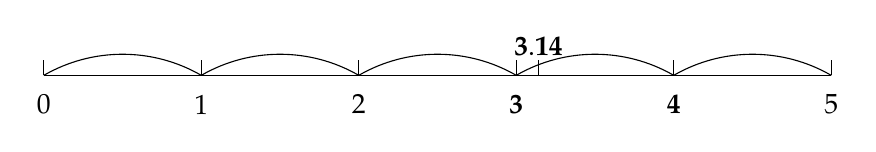
\begin{tikzpicture}[scale=2.0]
        \coordinate (O) at (0,0);
        \coordinate (I) at (1,0);
        \coordinate (II) at (2,0);
        \coordinate (III) at (3,0);
        \coordinate (IV) at (4,0);
        \coordinate (V) at (5,0);

        \coordinate (PI) at (3.1415926,0);

        \node [label={below:$0$}] at (O) {};
        \node [label={below:$1$}] at (I) {};
        \node [label={below:$2$}] at (II) {};
        \node [label={below:$\mathbf{3}$}] at (III) {};
        \node [label={above:$\mathbf{3.14}$}] at (PI) {};
        \node [label={below:$\mathbf{4}$}] at (IV) {};
        \node [label={below:$5$}] at (V) {};

        \draw (O) -- (I) -- (II) -- (III) -- (IV) -- (V);
        \draw (O) -- ++(0,0.1);
        \draw (I) -- ++(0,0.1);
        \draw (II) -- ++(0,0.1);
        \draw (III) -- ++(0,0.1);
        \draw (PI) -- ++(0,0.1);
        \draw (IV) -- ++(0,0.1);
        \draw (V) -- ++(0,0.1);

        \draw (O) arc (120:60:1);
        \draw (I) arc (120:60:1);
        \draw (II) arc (120:60:1);
        \draw (III) arc (120:60:1);
        \draw (IV) arc (120:60:1);
    \end{tikzpicture}
    \caption{Minh họa thuộc tính Archimedes với $x = 3.14$.}
\end{figure}

\begin{theorem}[Phần nguyên của số thực\index{Phần nguyên của số thực}]
    Với mọi số thực $x$, tồn tại duy nhất số nguyên $n$ sao cho $n\leq x < n+1$.

    \noindent Nói riêng, số nguyên $n$ như vậy được gọi là \textbf{phần nguyên của số thực $x$} và được kí hiệu là $\floor{x}$.
\end{theorem}

\begin{proof}
    Theo thuộc tính Archimedes, tồn tại số nguyên $a$ và $b$ sao cho $x < b$ và $-x < a$, kéo theo $-a < x < b$.

    Theo tính chất bắc cầu của quan hệ thứ tự trên tập hợp số thực, nếu một số nguyên $c$ thỏa mãn $c\leq x$ thì $c\leq b$. Theo nguyên lý thứ tự tốt, tập hợp các số nguyên nhỏ hơn hoặc bằng $x$ có phần tử lớn nhất, chúng ta kí hiệu phần tử đó là $n$. Vì $n < n + 1$ và $n + 1$ là một số nguyên nên theo định nghĩa của $n$, chúng ta có $n\leq x < n + 1$.

    Giả sử số nguyên $m$ thỏa mãn $m\leq x < m + 1$. Giả sử phản chứng rằng $m < n$, khi đó $m + 1\leq n$, kéo theo $m + 1\leq x$, mâu thuẫn với $x < m + 1$. Giả sử phản chứng rằng $n < m$, khi đó $n + 1\leq m$, kéo theo $n + 1\leq x$, mâu thuẫn với $x < n + 1$. Do đó $m = n$.

    Vậy với mọi số thực $x$, tồn tại duy nhất số nguyên $n$ sao cho $n\leq x < n+1$.
\end{proof}

\begin{theorem}[Tính trù mật của tập hợp số hữu tỉ\index{Tính trù mật của tập hợp số hữu tỉ}]
    Với mọi số thực $x, y$ sao cho $x < y$, tồn tại số hữu tỉ $q$ sao cho $x < q < y$.
\end{theorem}

\begin{proof}
    Theo thuộc tính Archimedes, tồn tại số nguyên $n$ sao cho $1 < n(y - x)$. Do đó $1 + nx < ny$. Theo định nghĩa phần nguyên của số thực, chúng ta có $nx < \floor{nx} + 1 \leq nx + 1 < ny$.

    Do đó, với số nguyên $m = \floor{nx} + 1$, chúng ta có $nx < m < ny$. Bên cạnh đó, vì $y - x > 0$ và $n > 0$ nên  $1 < n(y - x)$ kéo theo $n > 0$. Do đó $x < \frac{m}{n} < y$.

    Vậy, với mọi số thực $x, y$ sao cho $x < y$, tồn tại số hữu tỉ $q$ sao cho $x < q < y$.
\end{proof}

\subsection{Bài tập}

\section{Số phức}

\subsection{Xây dựng tập hợp số phức}

\subsection{Phần thực, phần ảo, liên hợp của số phức}

\subsection{Biểu diễn hình học và dạng lượng giác của số phức}

\subsection{Bài tập}

\chapter{Số thực}\label{chapter:real-numbers}

\section{Số thực là gì?}

\subsection{Hệ tiên đề về số thực}

Có ít nhất hai cách hiểu cho câu hỏi ``Số thực là gì?\@'' Đầu tiên, chúng ta có thể hiểu rằng người hỏi đang muốn được biết một \textit{định nghĩa toán học} cho số thực. Đó là một định nghĩa hình thức tương tự như định nghĩa số tự nhiên, số nguyên, số hữu tỉ, tính chia hết, \ldots đã được nêu trong tài liệu này. Thứ hai, chúng ta có thể hiểu rằng người hỏi đang muốn liên hệ cái-được-gọi-là-số-thực với thực tế. Nói cách khác, để trả lời cho cách hiểu thứ hai, người trả lời cần định nghĩa số thực như một đối tượng nào đó tương đương trong thực tế hoặc gần thực tế.

Chúng tôi đưa ra một câu trả lời trực giác cho cách hiểu thứ hai như sau: \textit{Hình dung một đường thẳng kéo dài vô tận về hai phía. Mỗi điểm được đánh dấu trên đường thẳng đó tương ứng với một số thực. Nói rõ hơn, trên đường thẳng đó, chúng ta đánh dấu hai điểm khác nhau, lần lượt gọi là $0$ và $1$. Các điểm $x$ trên đường thẳng này tương ứng với một số (thực) âm nếu điểm $0$ nằm giữa $x$ và $1$. Các điểm $x$ trên đường thẳng này tương ứng với một số (thực) dương nếu hoặc $x$ nằm giữa $0$ và $1$, hoặc $x$ trùng $1$, hoặc $1$ nằm giữa $0$ và $x$.}

Câu trả lời trực giác hình học cho cách hiểu thứ hai có thể làm hài lòng nhiều người nhưng là không đủ tốt đối với một định nghĩa toán học. Với định nghĩa trực giác như vậy, chúng ta khó lòng nói về các phép toán với các số thực như cộng, trừ, nhân, chia. Đối với những người học và làm toán, việc biết các số thực và các phép toán với số thực, quan hệ giữa các số thực có những tính chất gì quan trọng hơn việc biết số thực là gì trong thực tế. Trong chương này, chúng ta định nghĩa số thực bằng một hệ tiên đề (hay tính chất). Chúng ta coi những đối tượng thỏa mãn hệ tiên đề (hay tính chất) này là các số thực.

\begin{axiom}
    Tập hợp số thực được kí hiệu là $\mathbb{R}$. Các phần tử của $\mathbb{R}$ thỏa mãn ba nhóm tiên đề sau.

    \textbf{Các tiên đề về trường.} $\mathbb{R}$ có hai phép toán hai ngôi là phép cộng (được kí hiệu là $+$) và phép nhân (được kí hiệu là $\cdot$) và các phép toán này thỏa mãn các tính chất sau:
    \begin{enumerate}[label={(\roman*)}]
        \item Phép cộng có tính chất kết hợp. Nói cách khác, với mọi số thực $x, y, z$, chúng ta có
              \[
                  (x + y) + z = x + (y + z).
              \]
        \item Phép cộng có phần tử đồng nhất. Nói cách khác, tồn tại số thực $0$ sao cho với mọi số thực $x$, chúng ta có
              \[
                  x + 0 = 0 + x = x.
              \]
        \item Mỗi số thực có phần tử đối. Nói cách khác, với mỗi số thực $x$, tồn tại số thực $(-x)$ thỏa mãn
              \[
                  x + (-x) = (-x) + x = 0.
              \]
        \item Phép cộng có tính chất giao hoán. Nói cách khác, với mọi số thực $x, y$, chúng ta có
              \[
                  x + y = y + x.
              \]
        \item Phép nhân có tính chất kết hợp. Nói cách khác, với mọi số thực $x, y, z$, chúng ta có
              \[
                  (x \cdot y) \cdot z = x \cdot (y \cdot z).
              \]
        \item Phép nhân có tính chất phân phối với phép cộng. Nói cách khác, với mọi số thực $x, y, z$, chúng ta có
              \[
                  \begin{split}
                      (x + y)\cdot z = x\cdot z + y\cdot z, \\
                      z\cdot (x + y) = z\cdot x + z\cdot y.
                  \end{split}
              \]

        \item Phép nhân có phần tử đồng nhất, phần tử này khác $0$. Nói cách khác, tồn tại số thực $1\ne 0$ sao cho với mọi số thực $x$, chúng ta có
              \[
                  x + 1 = 1 + x = x.
              \]
        \item Phép nhân có tính chất giao hoán. Nói cách khác, với mọi số thực $x, y$, chúng ta có
              \[
                  x\cdot y = y\cdot x.
              \]
        \item Mỗi số thực khác $0$ có phần tử nghịch đảo. Nói cách khác, với mỗi số thực $x\ne 0$, tồn tại số thực $x^{-1}$ sao cho
              \[
                  x\cdot x^{-1} = x^{-1}\cdot x = 1.
              \]
    \end{enumerate}

    \textbf{Các tiên đề về thứ tự.} $\mathbb{R}$ có quan hệ $\leq$ thỏa mãn các tính chất sau:
    \begin{enumerate}[label={(\roman*)}]
        \item $\leq$ là một quan hệ thứ tự toàn phần.
        \item Với mọi số thực $x, y$, nếu $x\leq y$ thì với mọi số thực $z$, chúng ta có $x + z\leq y + z$.
        \item Với mọi số thực $x, y$, nếu $0\leq x$ và $0\leq y$ thì $0\leq x\cdot y$.
    \end{enumerate}

    \textbf{Tiên đề về cận trên (hay tiên đề về tính đầy đủ).} Nếu một tập hợp con khác rỗng của $\mathbb{R}$ có cận trên thì cũng có cận trên nhỏ nhất.
\end{axiom}

Chúng ta bình luận và làm rõ thêm hệ tiên đề vừa nêu. Các tiên đề về trường và các tiên đề về thứ tự có lẽ không có gì xa lạ với bạn đọc. Chúng tôi chỉ lưu ý thêm ba điều về hai nhóm tiên đề này: (1) Các phần tử $0$, $1$, $(-x)$, và $x^{-1}$ được hiểu như các kí hiệu đơn thuần, ở thời điểm này chúng ta \textit{chưa} coi đó như những số hay phép toán quen thuộc; (2) Tiên đề về sự tồn tại của hai phần tử $0$ và $1$ không khẳng định tính duy nhất của những phần tử như vậy, chúng ta sẽ chứng minh tính duy nhất của hai phần tử đó ở một mục khác trong chương này.

Tiên đề về cận trên là phần ít quen thuộc nhất trong hệ tiên đề trên, và chúng ta cần làm rõ khái niệm được nhắc tới trong tiên đề này: \textit{cận trên} và \textit{cận trên nhỏ nhất}.

\begin{definition}[Cận trên và Cận dưới]
    Cho một tập hợp $S$ được định nghĩa một quan hệ thứ tự bộ phận $\leq$ và $A$ là một tập hợp con của $S$.
    \begin{enumerate}[label={(\roman*)}]
        \item Một phần tử $u$ của $S$ được gọi là một \textbf{cận trên\index{Cận trên}} của $A$ nếu như với mỗi phần tử $a$ của $A$, chúng ta có $a\leq u$. Chúng ta còn nói $A$ bị chặn trên bởi $u$.
        \item Một phần tử $\ell$ của $S$ được gọi là một \textbf{cận dưới\index{Cận dưới}} của $A$ nếu như với mỗi phần tử $a$ của $A$, chúng ta có $\ell\leq a$. Chúng ta còn nói $A$ bị chặn dưới bởi $\ell$.
        \item Tập hợp $A$ được gọi là bị chặn nếu $A$ có cả cận trên và cận dưới.
        \item Một phần tử $x$ của $S$ được gọi là một \textbf{cận trên nhỏ nhất\index{Cận trên nhỏ nhất}} hay \textbf{cận trên đúng\index{Cận trên đúng}} của $A$ nếu như với mỗi cận trên $u$ của $A$, chúng ta có $x\leq u$. Cận trên nhỏ nhất của $A$ được kí hiệu là $\sup A$.
        \item Một phần tử $y$ của $S$ được gọi là một \textbf{cận dưới lớn nhất\index{Cận dưới lớn nhất}} hay \textbf{cận dưới đúng\index{Cận dưới đúng}} của $A$ nếu như với mỗi cận dưới $\ell$ của $A$, chúng ta có $\ell\leq y$. Cận dưới lớn nhất của $A$ được kí hiệu là $\inf A$.
    \end{enumerate}
\end{definition}

Chúng ta theo dõi một số ví dụ.
\begin{example}
    Tập hợp
    \[
        S = \left\{ 1, \frac{1}{2}, \frac{1}{3}, \ldots \right\} = \left\{ \frac{1}{n} \mid \text{$n$ là một số nguyên dương} \right\}
    \]

    là một tập hợp con của tập hợp số hữu tỉ $\mathbb{Q}$. Tập hợp $\mathbb{Q}$ được sắp thứ tự toàn phần.
    \begin{itemize}
        \item $S$ bị chặn trên bởi $1, 2, \frac{5}{2}, 3, \ldots$ và bị chặn dưới bởi $0, \frac{-1}{2}, -1, \ldots$
        \item $1$ là cận trên nhỏ nhất của $S$.
        \item $S$ không có phần tử nhỏ nhất. Bởi vì mỗi phần tử $\frac{1}{m}$ của $S$, luôn có phần tử nhỏ hơn, chẳng hạn $\frac{1}{m+1}, \frac{1}{2m}, \ldots$
        \item $0$ là cận dưới lớn nhất của $S$. Giả sử phản chứng rằng $S$ có một cận dưới lớn hơn $0$. Cận dưới đó (là một số hữu tỉ vì chúng ta đang xét $S$ là tập hợp con của $\mathbb{Q}$). Chúng ta kí hiệu phân số tối giản của cận dưới đó là $\frac{p}{q}$. Nhưng vì $\frac{p}{q}\geq \frac{1}{q} > \frac{1}{2q}$ nên $\frac{p}{q}$ không phải cận dưới của $S$, dẫn đến giả sử phản chứng là sai. Do đó chúng ta khẳng định $0$ là cận dưới lớn nhất của $S$.
        \item $1$ vừa là cận trên nhỏ nhất, vừa là phần tử lớn nhất của $S$. Còn $0$ là cận dưới lớn nhất của $S$ nhưng không thuộc $S$, và do đó không phải phần tử nhỏ nhất của $S$.
    \end{itemize}
\end{example}

Quay lại với hệ tiên đề về số thực. Trong chương trước, chúng ta đã chỉ ra được tập hợp số hữu tỉ $\mathbb{Q}$ cùng với hai phép toán cộng, nhân, và quan hệ $\leq$ thỏa mãn các tiên đề về trường và các tiên đề về thứ tự. Mệnh đề dưới đây cho thấy tập hợp số hữu tỉ không thỏa mãn tiên đề về cận trên, hay chúng ta còn nói rằng tập hợp số hữu tỉ không đầy đủ theo quan hệ thứ tự $\leq$.

\begin{proposition}\label{proposition:irrational-cut}
    Trong tập hợp số hữu tỉ
    \begin{enumerate}[label={(\roman*)}]
        \item Chứng minh rằng không tồn tại số hữu tỉ $x$ nào thỏa mãn $x^{2} = 2$.
        \item Chứng minh rằng tập hợp
              \[
                  S = \{ x \mid x\in\mathbb{Q}, 0 < x \text{ và } x^{2} < 2 \}
              \]

              không có phần tử lớn nhất.
        \item Chứng minh rằng tập hợp $S$ ở phần (ii) không có cận trên nhỏ nhất.
    \end{enumerate}
\end{proposition}

\begin{proof}
    \begin{enumerate}[label={(\roman*)}]
        \item Giả sử phản chứng rằng tồn tại số hữu tỉ $x$ sao cho $x^{2} = 2$. Chúng ta kí hiệu phân số tối giản của $x$ là $\frac{p}{q}$. Vì ${\left(\frac{p}{q}\right)}^{2} = 2$ nên $p^{2} = 2q^{2}$. Vì $2$ là ước của $2q^{2}$ nên $2$ cũng là ước của $p^{2}$. Theo bổ đề Euclid (Định lý~\ref{theorem:euclid-lemma}), chúng ta suy ra $2$ là ước của $p$, do đó tồn tại số tự nhiên $a$ sao cho $p = 2a$. Cùng với việc $p^{2} = 2q^{2}$, chúng ta suy ra $4a^{2} = 2q^{2}$, kéo theo $2a^{2} = q^{2}$. Một lần nữa, theo bổ đề Euclid, chúng ta suy ra $2$ là ước của $q$. Như vậy $2$ là ước chung của $p$ và $q$, điều này mâu thuẫn với việc $\frac{p}{q}$ là một phân số tối giản.

              Vậy không tồn tại số hữu tỉ $x$ nào thỏa mãn $x^{2} = 2$.
        \item Chúng ta chọn một số hữu tỉ $\frac{a}{b}$ thuộc $S$ (trong đó $a, b$ là các số nguyên dương). Theo định nghĩa của $S$, chúng ta suy ra $a^{2} < 2b^{2}$. Xét số hữu tỉ $\frac{2a + 2b}{a + 2b}$.
              \begin{align*}
                  {(2a + 2b)}^{2} & = 4a^{2} + 8ab + 4b^{2}   \\
                                  & < 2a^{2} + 8ab + 8b^{2}   \\
                                  & = 2(a^{2} + 4ab + 4b^{2}) \\
                                  & = 2{(a + 2b)}^{2}
              \end{align*}

              Do đó $\frac{2a + 2b}{a + b}$ là một phần tử của $S$. Bên cạnh đó, $\frac{a}{b} < \frac{2a + 2b}{a + 2b}$, vì
              \begin{align*}
                  a(a + 2b) & = a^{2} + 2ab < 2ab + 2b^{2} = b(2a + 2b)
              \end{align*}

              Như vậy, với mỗi phần tử $x$ thuộc $S$, chúng ta luôn tìm được được một phần tử khác của $S$ nhưng lớn hơn $x$. Do đó tập hợp $S$ không có phần tử lớn nhất.
        \item Tập hợp $S$ có cận trên. Chẳng hạn, $2$ là một cận trên của $S$, bởi vì với mọi $x$ thuộc $S$, $x^{2} < 2 < 4$, kéo theo $(x - 2)(x + 2) < 0$, và $x < 2$. Mặt khác, nếu $y$ là một cận trên của $S$ thì $y > 0$.

              Tiếp theo, chúng ta chứng minh rằng nếu số hữu tỉ $y$ là một cận trên của $S$ thì $y^{2} > 2$. Giả sử phản chứng rằng $y^{2}\leq 2$. Theo phần (i), chúng ta suy ra $y^{2} < 2$, kéo theo $y$ là một phần tử của $S$. $y$ là một cận trên của $S$ và là một phần tử của $S$ thì $y$ cũng là phần tử lớn nhất của $S$. Điều này mâu thuẫn với kết quả đã chứng minh ở phần (ii). Do đó giả sử phản chứng là sai, và chúng ta suy ra $y^{2} > 2$.

              Chọn $y$ là một cận trên của $S$. Chúng ta kí hiệu $\frac{a}{b}$ là phân số của $y$ ($a, b$ là các số nguyên dương). Vì $y^{2} > 2$ nên $a^{2} > 2b^{2}$. Chúng ta tiếp tục xét số hữu tỉ $\frac{2a + 2b}{a + 2b}$.
              \begin{align*}
                  {(2a + 2b)}^{2} & = 4a^{2} + 8ab + 4b^{2}   \\
                                  & > 2a^{2} + 8ab + 8b^{2}   \\
                                  & = 2(a^{2} + 4ab + 4b^{2}) \\
                                  & = 2{(a + 2b)}^{2}
              \end{align*}

              Do đó $\frac{2a + 2b}{a + b}$ là một cận trên của $S$. Ngoài ra, $\frac{2a + 2b}{a + 2b} < \frac{a}{b}$, vì
              \begin{align*}
                  b(2a + 2b) = 2ab + 2b^{2} < 2ab + a^{2} = a(a + 2b)
              \end{align*}

              Như vậy với mỗi cận trên $y$ của $S$, chúng ta luôn tìm được một cận trên khác của $S$ và nhỏ hơn $y$. Do đó tập hợp $S$ không có cận trên nhỏ nhất.
    \end{enumerate}
\end{proof}

\subsection{Dẫn nhập về việc xây dựng tập hợp số thực}

Vì sao cần xây dựng tập hợp số thực? Ở đây chúng tôi dẫn ra khía cạnh giảng dạy và khía cạnh cơ sở toán học. Trong khía cạnh giảng dạy, việc chỉ dẫn cách xây dựng tập hợp số thực sẽ cho thấy mối liên hệ giữa đối tượng mới (tập hợp số thực) với các đối tượng quen thuộc hơn (tập hợp số hữu tỉ, tập hợp số nguyên, tập hợp số tự nhiên). Điều đó có ích hơn so với việc thừa nhận hệ tiên đề và coi tập hợp số thực như một công cụ tiện lợi một cách khó hiểu. Ở khía cạnh cơ sở toán học, những người làm toán cố gắng không thừa nhận quá nhiều thứ. Đúng là trong một thời gian dài, các nhà Toán học vẫn sử dụng phương pháp tiên đề và xuất phát từ các tiên đề cùng các luật logic để chứng minh các định lý. Nhưng tư tưởng của phương pháp tiên đề không chỉ đơn thuần là thừa nhận một số mệnh đề rồi áp dụng luật logic, mà còn là việc xuất phát từ một ít tiên đề rồi từ đó xây dựng nên tất cả những thứ khác. Nếu thừa nhận quá nhiều thì chúng ta chẳng biết được bao nhiêu.

Xây dựng tập hợp số thực là gì? Xây dựng tập hợp số thực là việc tạo ra một đối tượng toán học thỏa mãn hệ tiên đề về số thực. Chúng ta có thể so sánh hệ tiên đề về số thực với một bản thiết kế, khi đó việc xây dựng tập hợp số thực chính là tạo ra một công trình, tác phẩm giống như bản thiết kế đó. Xây dựng được tập hợp số thực đồng nghĩa với việc \textit{chứng minh} bản thiết kế là khả thi. Trong toán học, chúng ta có thuật ngữ riêng để gọi một công trình tương ứng với một bản thiết kế, đó là \textit{mô hình} và \textit{hệ tiên đề}. Mô hình là một đối tượng, hay cấu trúc toán học thỏa mãn một hệ tiên đề nào đó. Để minh họa, chúng tôi đưa ra một mô hình bằng lý thuyết tập hợp (được đề xuất bởi nhà toán học John von Neumann) cho hệ tiên đề Peano về số tự nhiên như sau:
\begin{itemize}
    \item $0$ là tập hợp rỗng $\varnothing$.
    \item $S$ là một phép toán trên tập hợp: $S(A) = A \cup \{ A \}$.
    \item Các số tự nhiên tương ứng với các tập hợp sau (dưới đây chỉ liệt kê bốn số tự nhiên)
          \begin{align*}
              0 & = \varnothing,                                                                                                \\
              1 & = 0 \cup \{ 0 \} = \{ \varnothing \},                                                                         \\
              2 & = 1 \cup \{ 1 \} = \{ 0, 1 \}  = \{ \varnothing, \{ \varnothing \} \}                                         \\
              3 & = 2 \cup \{ 2 \} = \{ 0, 1, 2 \} = \{ \varnothing, \{ \varnothing \}, \{ \varnothing, \{ \varnothing \} \} \}
          \end{align*}
    \item Quan hệ bằng nhau giữa các số tự nhiên được nhìn nhận là quan hệ bằng nhau giữa các tập hợp.
\end{itemize}

Việc kiểm tra một mô hình có thỏa mãn một hệ tiên đề hay không chính là công việc chứng minh.

Chỉ còn lại câu hỏi là làm sao để xây dựng tập hợp số thực. Hiện nay, hai cách xây dựng tập hợp số thực thường được sử dụng nhất là \textit{lát cắt Dedekind} và \textit{dãy Cauchy hữu tỉ}, với cơ sở là tập hợp số hữu tỉ. Trong chương này, chúng tôi giải thích ý tưởng và nêu chi tiết về cả hai cách xây dựng. Cách xây dựng được trình bày trong chương này mang nhiều chi tiết kĩ thuật, đặc biệt là với dãy Cauchy hữu tỉ. Chúng tôi khuyên bạn đọc theo dõi những kết quả chính trước (được đánh dấu là Định lý), chú ý tới thứ tự, bình luận, và không cần nắm bắt chứng minh của tất cả trong lần đọc đầu tiên.

\section{Lát cắt Dedekind}

Trong mục này, không gian mà chúng ta làm việc (định nghĩa và chứng minh các kết quả liên quan đến lát cắt Dedekind) là tập hợp số hữu tỉ.

\subsection{Định nghĩa lát cắt Dedekind}

Trong phần mở đầu của chương này, chúng tôi có đưa ra một định nghĩa trực giác về tập hợp số thực. Theo định nghĩa trực giác đó, tập hợp số thực là một đường thẳng kéo dài vô tận về hai phía, còn mỗi số thực tương ứng với một điểm được đánh dấu trên đường thẳng đó. Định nghĩa trực giác này có thể được xem như khởi nguồn cho định nghĩa lát cắt Dedekind sau đây.

\begin{definition}[Lát cắt Dedekind]
    Một lát cắt Dedekind\index{Lát cắt Dedekind} trong một tập hợp $S$ được sắp thứ tự toàn phần là một phân hoạch gồm hai tập hợp $A, B$ sao cho
    \begin{enumerate}[label={(DC\arabic*)}]
        \item $A$ khác rỗng và $A$ không phải toàn bộ tập hợp $S$.
        \item Mọi phần tử của $A$ nhỏ hơn mọi phần tử của $B$.
        \item $A$ không có phần tử lớn nhất.
        \item Nếu $x$ thuộc $A$ thì bất cứ phần tử nào nhỏ hơn $x$ và thuộc $S$ cũng thuộc $A$ (đặc điểm này còn được phát biểu là $A$ đóng dưới).
    \end{enumerate}

    Một lát cắt như vậy được kí hiệu là $(A, B)$, hoặc chỉ là $A$, bởi vì $B = S\setminus A$ ($B$ hoàn toàn được xác định khi biết $A$).

    Chúng ta kí hiệu tập hợp các lát cắt Dedekind trong tập hợp $S$ là $\mathscr{D}_{S}$.
\end{definition}

Để xây dựng tập hợp số thực bằng lát cắt Dedekind, chúng ta sử dụng các lát cắt trong tập hợp số hữu tỉ. Tập hợp các lát cắt Dedekind trong tập hợp số hữu tỉ được kí hiệu là $\mathscr{D}_{\mathbb{Q}}$. Chúng ta cũng dùng cách gọi vắn tắt là lát cắt để chỉ lát cắt Dedekind trên tập hợp số hữu tỉ, trừ khi ngữ cảnh phát biểu khác đi.

Để hiểu rõ hơn định nghĩa lát cắt, chúng ta theo dõi các ví dụ và phản ví dụ sau.
\begin{example}
    Tập hợp
    \[
        A = \{ x \mid x\in\mathbb{Q} \wedge x < q \}
    \]

    trong đó $q$ là một số hữu tỉ, là một lát cắt. Chúng ta kiểm tra điều này qua từng điều trong định nghĩa lát cắt.
    \begin{enumerate}[label={(DC\arabic*)}]
        \item $A$ khác rỗng vì $q - 1$ là một phần tử của $A$. Bên cạnh đó, $A$ cũng không phải toàn bộ tập hợp số hữu tỉ vì $q$ không phải một phần tử của $A$.
        \item $B = \mathbb{Q} - A = \{ x \mid x\in\mathbb{Q} \wedge q\leq x \}$. Mọi phần tử của $A$ nhỏ hơn mọi phần tử của $B$ theo tính chất bắc cầu của quan hệ $\leq$ trên tập hợp số hữu tỉ.
        \item $A$ không có phần tử lớn nhất vì với mỗi phần tử $x$ của $A$, chúng ta luôn tìm được một phần tử khác lớn hơn, chẳng hạn như $\frac{q + x}{2}$.
        \item Nếu một số hữu tỉ $x$ thuộc $A$ thì mọi số hữu tỉ nhỏ hơn $x$ cũng thuộc $A$. Điều này được suy ra từ tính chất bắc cầu của quan hệ $\leq$ trên tập hợp số hữu tỉ.
    \end{enumerate}
\end{example}

\begin{example}
    Tập hợp
    \[
        A = \{ x \mid \text{$x$ là số hữu tỉ thỏa mãn $x < 0$ hoặc $x^{2} < 2$} \}
    \]

    là một lát cắt. Điều này được suy ra từ tính chất bắc cầu của quan hệ $\leq$ trên tập hợp số hữu tỉ và Mệnh đề~\ref{proposition:irrational-cut}.
\end{example}

\begin{counterexample}
    Tập hợp
    \[
        A = \{ x \mid \text{$x$ là số hữu tỉ thỏa mãn $x > 0$ và $x^{2} < 2$} \}
    \]

    \textbf{không phải} một lát cắt. Bởi vì $1$ là phần tử của $A$ nhưng $0 < 1$ lại không phải một phần tử của $A$.
\end{counterexample}

\begin{counterexample}
    Tập hợp
    \[
        A = \left\{ \frac{-1}{n} \mid \text{$n$ là một số nguyên dương} \right\}
    \]

    \textbf{không phải} một lát cắt. Bởi vì $-1$ là phần tử của $A$ nhưng $-2 < -1$ lại không phải một phần tử của $A$.
\end{counterexample}

\noindent Trước khi tiếp tục xây dựng tập hợp số thực bằng lát cắt, chúng ta lưu ý kết quả sau về lát cắt nói chung.
\begin{proposition}\label{proposition:upper-bound-of-dedekind-cut}
    Tập hợp $A$ là tập hợp con của một tập hợp $S$ được sắp thứ tự toàn phần sao cho $A$ khác rỗng và $A$ không phải toàn bộ tập hợp $S$. Chứng minh rằng $A$ là một lát cắt khi và chỉ khi $S\setminus A$ chỉ chứa tất cả các cận trên của $A$.
\end{proposition}

\begin{proof}
    ($\Rightarrow$) $A$ là một lát cắt.

    Theo định nghĩa lát cắt, mọi phần tử của $A$ nhỏ hơn mọi phần tử của $S\setminus A$. Do đó mọi phần tử của $S\setminus A$ là các cận trên của $A$.

    Giả sử phản chứng rằng nếu phần tử $x$ của $S$ là một cận trên của $A$ thì $x$ thuộc $A$. Theo giả sử phản chứng, $x$ là phần tử lớn nhất của $A$, và điều này mâu thuẫn với định nghĩa lát cắt rằng $A$ không có phần tử lớn nhất. Do đó giả sử phản chứng là sai, kéo theo mọi cận trên của $A$ là phần tử của $S - A$.

    Do đó $S\setminus A$ chỉ chứa tất cả các cận trên của $A$.

    \bigskip

    ($\Leftarrow$) $S\setminus A$ chỉ chứa tất cả các cận trên của $A$.

    Giả sử phản chứng rằng $A$ có phần tử lớn nhất. Chúng ta kí hiệu phần tử lớn nhất của $A$ là $x$. Vì $x$ là một cận trên của $A$ nên $x$ cũng là một phần tử của $S\setminus A$. Điều này mâu thuẫn với định nghĩa hiệu của hai tập hợp. Do đó giả sử phản chứng là sai, kéo theo $A$ không có phẩn tử lớn nhất.

    Giả sử $a\in A$ và $x < a$. Vì $x < a$ nên $x$ không phải cận trên của $A$, kéo theo $x$ không phải phần tử của $S\setminus A$. Do đó $x$ là một phần tử của $A$.

    Theo định nghĩa lát cắt, chúng ta kết luận $A$ là một lát cắt.
\end{proof}

Trong các mục tiếp theo, chúng ta lần lượt định nghĩa quan hệ thứ tự giữa các lát cắt, phép toán cộng, nhân hai lát cắt và kiểm tra xem những cấu trúc đó có thỏa mãn hệ tiên đề về số thực hay không.

\subsection{Quan hệ thứ tự giữa các lát cắt}

Việc hình dung tập hợp số thực như một đường thẳng cho chúng ta một cách nhìn khá trực quan về quan hệ thứ tự (tương ứng với khái niệm bên trái, bên phải trong thực tế).

\begin{definition}\label{definition:order-relation-between-dedekind-cuts}
    $A$ và $B$ là hai lát cắt. Chúng ta nói lát cắt $A$ có quan hệ $\leq$ với lát cắt $B$ và kí hiệu là $A\leq B$ nếu và chỉ nếu $A\subseteq B$.
\end{definition}

\begin{theorem}
    Quan hệ $\leq$ trên tập hợp các lát cắt $\mathscr{D}_{\mathbb{Q}}$ ở Định nghĩa~\ref{definition:order-relation-between-dedekind-cuts} là một quan hệ thứ tự toàn phần.
\end{theorem}

\begin{proof}
    Với mỗi lát cắt $A$, chúng ta luôn có $A\subseteq A$, kéo theo $A\leq A$. Do đó quan hệ $\leq$ trên tập hợp $\mathscr{D}_{\mathbb{Q}}$ có tính chất phản xạ.

    Với mỗi lát cắt $A, B, C$, nếu $A\leq B$ và $B\leq C$ thì $A\subseteq B$ và $B\subseteq C$. Vì quan hệ bao hàm giữa các tập hợp có tính chất bắc cầu nên $A\subseteq C$, kéo theo $A\leq C$. Do đó quan hệ $\leq$ trên tập hợp $\mathscr{D}_{\mathbb{Q}}$ có tính chất bắc cầu.

    Với mỗi lát cắt $A, B$, nếu $A\leq B$ và $B\leq A$ thì $A\subseteq B$ và $B\subseteq A$, kéo theo $A = B$. Do đó quan hệ $\leq$ trên tập hợp $\mathscr{D}_{\mathbb{Q}}$ có tính chất phản đối xứng.

    Như vậy quan hệ $\leq$ trong tập hợp các lát cắt $\mathscr{D}_{\mathbb{Q}}$ là một quan hệ thứ tự.

    \bigskip

    Chúng ta chọn hai lát cắt $A, B$ bất kì. Nếu $A = B$ thì $A\leq B$ và $B\leq A$. Nếu $A\ne B$, chúng ta xét hai trường hợp sau.
    \begin{enumerate}[label={\textbf{Trường hợp \arabic*.}},itemindent=2cm]
        \item Mọi phần tử của $A$ đều thuộc $B$.

              Điều này đồng nghĩa với $A\subset B$, kéo theo $A\leq B$.
        \item Tồn tại một phần tử của $A$ nhưng không thuộc $B$.

              Giả sử phần tử $a$ của $A$ không thuộc $B$. Theo Mệnh đề~\ref{proposition:upper-bound-of-dedekind-cut}, $a$ là một cận trên của $B$. Mà $B$ không có phần tử lớn nhất, nên chúng ta suy ra mọi phần tử của $B$ đều nhỏ hơn $a$. Vì $A$ là một lát cắt nên mọi số hữu tỉ nhỏ hơn $a$ đều thuộc $A$. Kết hợp hai điều vừa thu được, chúng ta suy ra mọi phần tử của $B$ đều là phần tử của $A$. Do đó $B\subset A$, kéo theo $B\leq A$.
    \end{enumerate}

    Do đó với hai lát cắt $A, B$ bất kì, $A\leq B$ hoặc $B\leq A$. Vậy quan hệ $\leq$ trên tập hợp các lát cắt $\mathscr{D}_{\mathbb{Q}}$ là một quan hệ thứ tự toàn phần.
\end{proof}

Chúng ta đặc biệt lưu ý lát cắt sau.
\[
    \begin{split}
        O = \{ x \mid x\in\mathbb{Q} \wedge x < 0 \}.
    \end{split}
\]

Với cơ sở là quan hệ thứ tự toàn phần trên tập hợp các lát cắt $\mathscr{D}_{\mathbb{Q}}$, chúng ta đưa ra định nghĩa sau.
\begin{definition}
    \begin{enumerate}[label={(\roman*)}]
        \item Một lát cắt $A$ được gọi là lát cắt dương nếu và chỉ nếu $O < A$.
        \item Một lát cắt $A$ được gọi là lát cắt âm nếu và chỉ nếu $A < O$.
    \end{enumerate}
\end{definition}

Như vậy, một lát cắt $A$ là không âm nếu và chỉ nếu $O\leq A$, là không dương nếu $A\leq O$.

\begin{theorem}
    Nếu lát cắt $A$ là một lát cắt dương thì tồn tại một phần tử $a$ của $A$ sao cho $a > 0$.
\end{theorem}

\begin{proof}
    Giả sử phản chứng rằng lát cắt dương $A$ không có số hữu tỉ dương nào. Như vậy mọi phần tử $x$ của $A$ đều thỏa mãn $x\leq 0$. Do đó, $A\subseteq O$. Theo định nghĩa quan hệ $\leq$ trên tập hợp $\mathscr{D}_{\mathbb{Q}}$, chúng ta suy ra $A\leq O$. Điều này mâu thuẫn với giả thiết $A$ là một lát cắt dương ($A > O$).

    Vậy nếu lát cắt $A$ là một lát cắt dương thì tồn tại một phần tử $a$ của $A$ sao cho $a > 0$.
\end{proof}

\subsection{Phép cộng lát cắt}

\begin{theorem}[Phép toán cộng lát cắt]
    Cho hai lát cắt $A$ và $B$. Khi đó tập hợp sau
    \[
        A + B = \{ a + b \mid a\in A\wedge b\in B \}
    \]

    là một lát cắt.
\end{theorem}

\begin{proof}
    Chúng ta kiểm tra từng điều kiện của một lát cắt.
    \begin{enumerate}[label={(DC\arabic*)}]
        \item Vì $A$ và $B$ khác rỗng nên tồn tại hai số hữu tỉ $a$ và $b$ lần lượt thuộc $A$ và $B$. Theo định nghĩa của tập hợp $A + B$ thì $a + b$ là một phần tử của $A + B$. Do đó tập hợp $A + B$ khác rỗng.
        \item Chúng ta chọn $c$ là một cận trên của $A$, và $d$ là một cận trên của $B$. Với mọi phần tử $a$ thuộc $A$ và $b$ thuộc $B$, chúng ta có $a + b\leq c + b \leq c + d$. Do đó $A + B$ không phải toàn bộ tập hợp số hữu tỉ.
        \item Chúng ta chọn $a + b$ là một phần tử bất kì của tập hợp $A + B$, trong đó $a$ thuộc $A$ và $b$ thuộc $B$. Vì $A$ là một lát cắt nên $A$ không có phần tử lớn nhất, do đó tồn tại phần tử $a'$ của $A$ sao cho $a < a'$. Từ việc $a < a'$, chúng ta suy ra $a + b < a' + b$. Do đó trong tập hợp $A + B$, với mỗi phần tử, luôn tồn tại phần tử lớn hơn, kéo theo $A + B$ không có phần tử lớn nhất.
        \item Chúng ta chọn $a + b$ là một phần tử bất kì của tập hợp $A + B$, và $x$ là một số hữu tỉ nhỏ hơn $a + b$. Vì $x < a + b$ nên $x + (-b) < a$. Theo định nghĩa lát cắt, vì $x + (-b) < a$ nên $x + (-b)$ thuộc $A$. Theo định nghĩa của tập hợp $A + B$, $x = (x + (-b)) + b$ là một phần tử của $A + B$. Do đó $A + B$ đóng dưới.
    \end{enumerate}

    Vậy $A + B$ là một lát cắt.
\end{proof}

Sau đây, chúng ta kiểm tra bốn tiên đề đầu tiên của các tiên đề về trường. Chúng tôi gặp khó khăn với việc kiểm tra tiên đề thứ ba trong các tiên đề về trường. Để giải quyết khó khăn đó, chúng tôi sử dụng một tính chất sâu hơn của số hữu tỉ. Định nghĩa trong mệnh đề sau còn được sử dụng ở những phần sau của tài liệu.

\begin{proposition}[Phần nguyên của số hữu tỉ]\label{proposition:integral-part-of-rational-numbers}
    Với mỗi số hữu tỉ $x$, tồn tại duy nhất số nguyên $k$ sao cho $k\leq x < k+1$. (Số nguyên $k$ như vậy được gọi là \textbf{phần nguyên\index{Phần nguyên}} của số hữu tỉ $x$, và được kí hiệu là $\floor{x}$.)
\end{proposition}

\begin{proof}
    Chúng ta kí hiệu $\frac{a}{b}$ là phân số tối giản của $x$ (lưu ý rằng $b$ là một số nguyên dương). Theo thuật toán chia Euclid, tồn tại duy nhất số nguyên $k$ và số nguyên $r$ sao cho $a = kb + r$ và $0\leq r < b$. Do đó
    \[
        k = \frac{kb}{b} \leq \frac{kb + r}{b} = \frac{a}{b} < \frac{(k+1)b}{b} = k+1
    \]

    Giả sử số nguyên $\ell$ thỏa mãn $\ell\leq x < \ell + 1$.

    Giả sử phản chứng rằng $\ell < k$. Khi đó $\ell\leq k - 1$. Cùng với $x < \ell + 1$, chúng ta suy ra $x < \ell + 1\leq (k-1) + 1 = k$. Điều này mâu thuẫn với $k\leq x$.

    Giả sử phản chứng rằng $\ell > k$. Khi đó $k\leq \ell - 1$. Cùng với $x < k + 1$, chúng ta suy ra $x < k + 1\leq (\ell - 1) + 1 = \ell$. Điều này mâu thuẫn với $\ell\leq x$.

    Do đó, $k = \ell$. Như vậy, với mỗi số hữu tỉ $x$, tồn tại duy nhất số tự nhiên $k$ sao cho $k\leq x < k+1$.
\end{proof}

Chứng minh các đẳng thức về lát cắt đồng nghĩa với việc chứng minh hai tập hợp bằng nhau. Nhắc lại, để chứng minh hai tập hợp bằng nhau, chúng ta cần chỉ ra tập hợp này là bộ phận của tập hợp kia và ngược lại, hoặc chỉ ra định nghĩa của hai tập hợp đó là tương đương.

\begin{theorem}[Các tính chất của phép cộng lát cắt]\label{theorem:properties-of-dedekind-cuts-addition}
    Trong tập hợp các lát cắt $\mathscr{D}_{\mathbb{Q}}$
    \begin{enumerate}[label={(\roman*)}]
        \item Phép toán cộng lát cắt có tính chất kết hợp. Nói cách khác, với mọi lát cắt $A, B, C$, chúng ta có
              \[
                  (A + B) + C = A + (B + C).
              \]
        \item Phép toán cộng lát cắt có phần tử đồng nhất. Nói cách khác, tồn tại lát cắt $O$ sao cho với mọi lát cắt $A$, chúng ta có
              \[
                  A + O = O + A = A.
              \]
        \item Mỗi lát cắt có một lát cắt đối. Nói cách khác, với mỗi lát cắt $A$, tồn tại lát cắt $A'$ sao cho
              \[
                  A + A' = A' + A = O.
              \]
        \item Phép cộng lát cắt có tính chất giao hoán. Nói cách khác, với mọi lát cắt $A, B$, chúng ta có
              \[
                  A + B = B + A.
              \]
    \end{enumerate}
\end{theorem}

\begin{proof}
    \begin{enumerate}[label={(\roman*)}]
        \item Theo định nghĩa phép cộng lát cắt và tính chất kết hợp của phép cộng số hữu tỉ
              \begin{align*}
                  (A + B) + C & = \{ x + c \mid x\in A + B \wedge c\in C \}                  \\
                              & = \{ (a + b) + c \mid (a\in A\wedge b\in B)\wedge c\in C \}  \\
                              & = \{ a + (b + c) \mid a\in A \wedge (b\in B\wedge c\in C) \} \\
                              & = \{ a + y \mid a\in A \wedge y\in B + C \}                  \\
                              & = A + (B + C).
              \end{align*}

              Do đó phép cộng lát cắt có tính chất kết hợp.
        \item Chúng ta định nghĩa lát cắt $O$ là tập hợp các số hữu tỉ nhỏ hơn $0$.

              Với mỗi phần tử $a + x$ của lát cắt $A + O$ ($a$ thuộc $A$ và $x$ thuộc $O$), chúng ta có $a + x < a$. Do đó $A + O \subseteq A$. Mặt khác, trong lát cắt $A$, với mỗi phần tử $a$, tồn tại một phần tử $a'$ sao cho $a < a'$. Chúng ta có $a = a' + ((-a') + a)$. $a'$ là một phần tử của $A$ và $(-a') + a$ là một phần tử của $A + O$. Do đó $A \subseteq A + O$. Như vậy, $A + O = A$.

              Hoàn toàn tương tự, với mỗi phần tử $x + a$ của lát cắt $O + A$ ($x$ thuộc $O$ và $a$ thuộc $A$), chúng ta có $x + a < a$. Do đó $O + A \subseteq A$. Mặt khác, trong lát cắt $A$, với mỗi phần tử $a$, tồn tại một phần tử $a'$ sao cho $a < a'$. Chúng ta có $a = (a + (-a')) + a'$. $a'$ là một phần tử của $A$ và $a + (-a')$ là một phần tử của $O + A$. Do đó $A \subseteq O + A$. Như vậy, $O + A = A$.
        \item Chúng ta định nghĩa tập hợp $A'$ như sau
              \[
                  A' = \{ x - a' \mid x < 0 \wedge a'\in \mathbb{Q} - A \}
              \]

              Trước tiên, chúng ta chứng minh rằng $A'$ là một lát cắt.
              \begin{enumerate}[label={(DC\arabic*)}]
                  \item Vì $A$ là một lát cắt nên $\mathbb{Q} - A$ khác rỗng. Chọn $a'$ thuộc $\mathbb{Q} - A$ và chọn $x$ là một số hữu tỉ nhỏ hơn $0$. Theo định nghĩa của tập hợp $A'$, $x - a'$ thuộc $A'$. Do đó $A'$ khác rỗng.
                  \item Giả sử $x - a'$ là một phần tử của $A'$ ($x < 0$ và $a'$ thuộc $\mathbb{Q} - A$). Chọn $a$ là một phần tử của $A$. Chúng ta có $x < 0$ và $a < a'$. Điều này kéo theo $-a' < -a$ và $x - a' < 0 - a = -a$. Như vậy $-a$ là một cận trên của $A'$. Do đó $A'$ không phải toàn bộ tập hợp số hữu tỉ.
                  \item Giả sử $x - a'$ là một phần tử của $A'$ ($x < 0$ và $a'$ thuộc $\mathbb{Q} - A$). Vì $O$ là một lát cắt nên tồn tại một số hữu tỉ $y$ nhỏ hơn $0$ và lớn hơn $x$. Vì $x - a'$ thuộc $A'$ và $x < y$ nên $x - a' < y - a'$. Phần tử $y - a'$ của $A'$ lớn hơn $x - a'$. Điều này có nghĩa là trong tập hợp $A'$, với mỗi phần tử, luôn tồn tại phần tử lớn hơn. Do đó $A'$ không có phần tử lớn nhất.
                  \item Giả sử $x - a'$ là một phần tử của $A'$ ($x < 0$ và $a'$ thuộc $\mathbb{Q} - A$) và số hữu tỉ $y$ thỏa mãn $y < x - a'$. Khi đó $(a' - x) + y < 0$ và
                        \[
                            y = ((x - a') + (a' - x)) + y = (x + ((a' - x) + y)) - a'
                        \]

                        Vì $x + ((a' - x) + y) < x + 0 < 0$ và $a'$ thuộc $\mathbb{Q} - A$ nên theo định nghĩa của tập hợp $A'$, chúng ta suy ra $y$ thuộc $A'$. Do đó $A'$ đóng dưới.
              \end{enumerate}

              Như vậy $A'$ là một lát cắt. Tiếp theo, chúng ta chứng minh $A + A' = A' + A = O$.

              Giả sử $a + (x - a')$ là một phần tử của $A + A'$ (trong đó $a$ thuộc $A$, $x < 0$, và $a'$ thuộc $\mathbb{Q} - A$). Vì $a - a' < 0$ và $x < 0$ nên $a + (x - a') = x + (a - a') < x < 0$. Do đó $A + A' \subseteq O$.

              Giả sử $(x - a') + a$ là một phần tử của $A + A'$ (trong đó $a$ thuộc $A$, $x < 0$, và $a'$ thuộc $\mathbb{Q} - A$). Vì $a - a' < 0$ và $x < 0$ nên $(x - a') + a = x + (a - a') < x < 0$. Do đó $A' + A \subseteq O$.

              Để chứng minh $O\subseteq A + A'$ và $O\subseteq A' + A$, chúng ta sẽ chỉ ra sự tồn tại của hai phần tử lần lượt thuộc $A$ và $A'$ sao cho tổng của chúng nhỏ hơn $0$.

              Giả sử $x$ là một số hữu tỉ nhỏ hơn $0$ và $a$ là một phần tử của $A$. Chúng ta xét tập hợp $S$ gồm tất cả các số nguyên $n$ sao cho $nx$ thuộc $A$.
              \[
                  S = \{ n \mid n\in\mathbb{Z} \wedge nx\in A \}
              \]

              Theo Mệnh đề~\ref{proposition:integral-part-of-rational-numbers}, với mỗi số hữu tỉ $q$, tồn tại số nguyên $k$ sao cho $k\leq \frac{q}{x} < k + 1$. Vì $x < 0$ nên
              \[
                  \begin{split}
                      (k + 1)x < \frac{q}{x}\cdot x = q, \\
                      kx \geq \frac{q}{x}\cdot x = q.
                  \end{split}
              \]

              Chọn $q$ là một phần tử của $A$ thì $(k + 1)x < q$ cho thấy tập hợp $S$ khác rỗng. Chọn $q$ là một cận trên của $A$ thì việc $kx\geq q$ cho thấy tập hợp $S$ không phải toàn bộ tập hợp số nguyên, tức là tồn tại số nguyên $n_{0}$ nào đó sao cho $n_{0}x$ không thuộc $A$.

              Bên cạnh đó, bằng định nghĩa của lát cắt, cùng tính chất phân phối của phép nhân với phép cộng số hữu tỉ và tính tương thích của phép cộng với quan hệ $\leq$ trên tập hợp số hữu tỉ, chúng ta rút ra hai nhận xét: (1) Nếu $n$ thuộc $S$ thì $(n + 1)$ cũng thuộc $S$; (2) Nếu $n$ không thuộc $S$ thì $(n - 1)$ cũng không thuộc $S$.

              Với những điều trên, chúng ta suy ra rằng với mọi $n$ thuộc $A$, chúng ta có $n\geq n_{0}$. Như vậy tập hợp $S$ thỏa mãn giả thiết của nguyên lý thứ tự tốt. Theo nguyên lý thứ tự tốt, $S$ có phần tử nhỏ nhất. Chúng ta kí hiệu phần tử nhỏ nhất của $S$ là $m$. Vì số nguyên $m$ là phần tử nhỏ nhất của $S$ nên $m - 1$ không thuộc $S$. Nói cách khác, $mx$ thuộc $A$ và $(m - 1)x$ không thuộc $A$. Do $A$ là một lát cắt, nên tồn tại phần tử $a$ của $A$ sao cho $mx < a$. Khi đó chúng ta có $mx - a < 0$. Ngoài ra
              \begin{align*}
                  x & = mx - (m-1)x = (a + (mx - a)) - (m-1)x \\
                    & = a + ((mx-a) - (m-1)x)                 \\
                    & = ((mx - a) - (m-1)x) + a
              \end{align*}

              Vì $a$ thuộc $A$ và $(mx - a) - (m-1)x$ thuộc $A'$ nên theo định nghĩa phép cộng lát cắt, chúng ta có $x$ thuộc $A + A'$ và $A' + A$. Vì chúng ta đang xét số hữu tỉ $x$ bất kì nhỏ hơn $0$, nên chúng ta suy ra $O \subseteq A + A'$ và $O \subseteq A' + A$.

              Như vậy, $O = A + A'$ và $O = A' + A$.
        \item Theo định nghĩa phép cộng lát cắt và tính chất giao hoán của phép cộng số hữu tỉ
              \begin{align*}
                  A + B & = \{ a + b \mid a\in A \wedge b\in B \} \\
                        & = \{ b + a \mid b\in B \wedge a\in A \} \\
                        & = B + A.
              \end{align*}

              Do đó phép cộng lát cắt có tính chất giao hoán.
    \end{enumerate}
\end{proof}

Với định lý sau đây, chúng ta khẳng định được tính duy nhất của phần tử đồng nhất của phép cộng lát cắt và lát cắt đối.
\begin{theorem}
    \begin{enumerate}[label={(\roman*)}]
        \item Phép cộng lát cắt có đúng một phần tử đồng nhất.
        \item Với mỗi lát cắt $A$, tồn tại duy nhất một lát cắt là lát cắt đối của $A$.
    \end{enumerate}
\end{theorem}

\begin{proof}
    \begin{enumerate}[label={(\roman*)}]
        \item Định lý~\ref{theorem:properties-of-dedekind-cuts-addition} đã chỉ ra sự tồn tại của phần tử đồng nhất của phép cộng lát cắt, phần tử đó là lát cắt $O$.

              Giả sử lát cắt $O'$ thỏa mãn $A + O' = O' + A = A$ với mọi lát cắt $A$. Khi đó, theo phần (i), (ii), (iii) của Định lý~\ref{theorem:properties-of-dedekind-cuts-addition} và định nghĩa của $O'$, chúng ta có $O' = O' + O = O$.

              Vậy phép cộng lát cắt có đúng một phần tử đồng nhất.
        \item Định lý~\ref{theorem:properties-of-dedekind-cuts-addition} đã chỉ ra rằng với mỗi lát cắt $A$, tồn tại một lát cắt $A'$ sao cho $A + A' = A' + A = O$.

              Giả sử lát cắt $A''$ thỏa mãn $A + A'' = A'' + A = O$. Khi đó, theo phần (i), (ii), (iii) của Định lý~\ref{theorem:properties-of-dedekind-cuts-addition} và định nghĩa của $A''$, chúng ta có
              \begin{align*}
                  A'' & = A'' + O        \\
                      & = A'' + (A + A') \\
                      & = (A'' + A) + A' \\
                      & = O + A'         \\
                      & = A'
              \end{align*}

              Vậy, với mỗi lát cắt $A$, tồn tại duy nhất một lát cắt là lát cắt đối của $A$.
    \end{enumerate}
\end{proof}

Với mỗi lát cắt $A$, chúng ta kí hiệu bởi $-A$ lát cắt sau
\[
    -A = A' = \{ x - a' \mid x < 0 \wedge a'\in \mathbb{Q} - A \}.
\]

\begin{theorem}\label{theorem:additive-inversion-is-involutive}
    Với mọi lát cắt $A$, chúng ta có $A = -(-A)$.
\end{theorem}

\begin{proof}
    Theo định nghĩa của $-A$ và phần (i), (ii), (iii) của Định lý~\ref{theorem:properties-of-dedekind-cuts-addition}
    \begin{align*}
        (-(-A)) & = (-(-A)) + O          \\
                & = (-(-A)) + ((-A) + A) \\
                & = ((-(-A)) + (-A)) + A \\
                & = O + A                \\
                & = A.
    \end{align*}

    Vậy, với mọi lát cắt $A$, chúng ta có $A = -(-A)$.
\end{proof}

Tiếp theo, chúng ta kiểm tra tính tương thích của phép cộng lát cắt với quan hệ thứ tự $\leq$ trên tập hợp $\mathscr{D}_{\mathbb{Q}}$.

\begin{theorem}
    Với mọi lát cắt $A, B$, nếu $A\leq B$ thì với mọi lát cắt $C$, chúng ta có $A + C\leq B + C$.
\end{theorem}

\begin{proof}
    Giả sử hai lát cắt $A, B$ thỏa mãn $A\leq B$. Theo định nghĩa quan hệ thứ tự $\leq$ trên tập hợp $\mathscr{D}_{\mathbb{Q}}$, chúng ta có $A\subseteq B$.

    Giả sử $a + c$ là một phần tử bất kì của $A + C$ (trong đó, $a$ thuộc $A$ và $c$ thuộc $C$). Vì $A\subseteq B$ nên $a$ thuộc $B$. Theo định nghĩa phép cộng lát cắt, chúng ta suy ra $a + c$ thuộc $B + C$. Do đó $A + C \subseteq B + C$.

    Vậy với mọi lát cắt $A, B$, nếu $A\leq B$ thì với mọi lát cắt $C$, chúng ta có $A + C\leq B + C$.
\end{proof}

Ngược lại, nếu các lát cắt $A, B, C$ thỏa mãn $A + C\leq B + C$ thì chúng ta cũng có $A\leq B$. Tuy nhiên đây là một hệ quả trực tiếp của định lý trên, bởi vì $A + C\leq B + C$ kéo theo $(A + C) + (-C) \leq (B + C) + (-C)$.

Kết hợp định lý trên với phương pháp chứng minh bằng phản chứng, chúng ta thu được các hệ quả sau.

\begin{corollary}
    \begin{enumerate}[label={(\roman*)}]
        \item Với mọi lát cắt $A, B$, nếu $A < B$ thì với mọi lát cắt $C$, chúng ta có $A + C < B + C$.
        \item Nếu $A$ và $B$ là các lát cắt không âm thì $A + B$ là một lát cắt không âm.
        \item Nếu $A$ và $B$ là các lát cắt dương thì $A + B$ là một lát cắt dương.
        \item Nếu $A$ và $B$ là các lát cắt âm thì $A + B$ là một lát cắt âm.
        \item Lát cắt $A$ là lát cắt dương khi và chỉ khi lát cắt $-A$ là lát cắt âm.
    \end{enumerate}
\end{corollary}

\begin{proposition}\label{proposition:nonnegative-elements-of-dedekind-cuts-addition}
    Với mọi lát cắt $A, B$, nếu $A > O$ và $B > O$ thì với mỗi số hữu tỉ $x$ không âm (nếu có) trong $A + B$, tồn tại số hữu tỉ $a$ không âm trong $A$ và số hữu tỉ $b$ không âm trong $B$ sao cho $x = a + b$.
\end{proposition}

\begin{proof}
    Vì phép cộng lát cắt có tính chất giao hoán nên không mất tính tổng quát, chúng ta giả sử $A\leq B$.

    Vì $A > O$ và $B > O$ nên $0$ là một phần tử của $A, B$ và trong $A, B$ tồn tại số hữu tỉ dương.

    Nếu số hữu tỉ $x$ thuộc $A + B$ và $x = 0$ thì $x = 0 + 0$.

    Nếu số hữu tỉ $x$ thuộc $A + B$ và $x > 0$, chúng ta xét các trường hợp sau và chỉ ra rằng $x$ có thể được viết dưới dạng tổng của hai số hữu tỉ không âm lần lượt thuộc $A$ và $B$.
    \begin{enumerate}[label={\textbf{Trường hợp \arabic*.}},itemindent=1.5cm]
        \item $A = B$.

              Giả sử phản chứng rằng $\frac{x}{2}$ không thuộc $A$ (và $B$). Khi đó $\frac{x}{2}$ là một cận trên của $A$ và $B$, kéo theo $x = \frac{x}{2} + \frac{x}{2}$ là một cận trên của $A + B$, điều này mâu thuẫn với giả thiết $x$ thuộc $A + B$. Do đó $\frac{x}{2}$ thuộc $A$ và $B$.
        \item $A < B$.

              \textbf{Khả năng 1.} $x$ thuộc $A$.

              $x$ thuộc $A$ thì $x$ cũng thuộc $B$ vì $A\subset B$, $\frac{x}{2}$ thuộc $A$ và $B$. Chúng ta viết $x = \frac{x}{2} + \frac{x}{2}$.

              \textbf{Khả năng 2.} $x$ không thuộc $A$ và $x$ thuộc $B$.

              Chúng ta viết $x = 0 + x$.

              \textbf{Khả năng 3.} $x$ không thuộc $A$ và không thuộc $B$.

              Theo định nghĩa tổng hai lát cắt, tồn tại phần tử $a$ của $A$ và phần tử $b$ của $B$ sao cho $x = a + b$. Nếu $a$ là số hữu tỉ âm thì $x < b$, kéo theo $x$ thuộc $B$ (vì $B$ đóng dưới). Nếu $b$ là số hữu tỉ âm thì $x < a$, kéo theo $x$ thuộc $A$ (vì $A$ đóng dưới). Việc $x$ thuộc $A$ hay $x$ thuộc $B$ đều mâu thuẫn với giả thiết. Do đó $a$ và $b$ là hai số hữu tỉ không âm. Do đó $x = a + b$ viết dưới dạng tổng của hai số hữu tỉ không âm lần lượt thuộc $A$ và $B$.
    \end{enumerate}

    Vậy với mọi lát cắt $A, B$, nếu $A > O$ và $B > O$ thì với mỗi số hữu tỉ $x$ không âm trong $A + B$, tồn tại số hữu tỉ $a$ không âm trong $A$ và số hữu tỉ $b$ không âm trong $B$ sao cho $x = a + b$.
\end{proof}

\subsection{Phép nhân lát cắt}

Khi định nghĩa phép nhân lát cắt, chúng ta cũng gặp vấn đề như khi định nghĩa phép nhân hai số nguyên. Trong trường này này, chúng ta cũng giải quyết tương tự như định nghĩa phép nhân hai số nguyên.

\begin{theorem}[Phép nhân hai lát cắt]
    Cho hai lát cắt $A$ và $B$.
    \begin{enumerate}[label={(\roman*)}]
        \item Nếu $A\geq O$ và $B\geq O$ thì tập hợp sau
              \[
                  A\cdot B = \{ ab \mid a\in A\wedge b\in B\wedge a\geq 0\wedge b\geq 0 \} \cup O
              \]

              là một lát cắt.
        \item Nếu $A\geq 0$ và $B < O$ thì tập hợp $A\cdot B = -A\cdot (-B)$ là một lát cắt.
        \item Nếu $A < 0$ và $B\geq O$ thì tập hợp $A\cdot B = -(-A)\cdot B$ là một lát cắt.
        \item Nếu $A < 0$ và $B < O$ thì tập hợp $A\cdot B = (-A)\cdot (-B)$ là một lát cắt.
    \end{enumerate}
\end{theorem}

\begin{proof}
    \begin{enumerate}[label={(\roman*)}]
        \item Chúng ta kiểm tra các điều kiện trong định nghĩa lát cắt.

              Nếu ít nhất một trong hai lát cắt $A$ và $B$ bằng $O$ thì tập hợp $\{ ab \mid a\in A\wedge b\in B\wedge a\geq 0\wedge b\geq 0 \}$ là tập hợp rỗng, kéo theo $A\cdot B = O$, và là một lát cắt.

              Dưới đây, chúng ta xét trường hợp $A > O$ và $B > O$.
              \begin{enumerate}[label={(DC\arabic*)}]
                  \item Theo định nghĩa của $A\cdot B$, $A\cdot B$ không phải tập hợp rỗng, vì $A\cdot B \supseteq O$ và $O$ khác rỗng.
                  \item $A > O$ và $B > O$ thì tập hợp $\{ ab \mid a\in A\wedge b\in B\wedge a\geq 0\wedge b\geq 0 \}$ khác rỗng. Vì $A$ và $B$ là các lát cắt nên $A$ và $B$ có cận trên. Chọn $a_{0}, b_{0}$ lần lượt là cận trên của $A$ và $B$. Vì $A > O, B > 0$ và $A, B$ không có phần tử lớn nhất nên $a_{0} > 0$ và $b_{0} > 0$. Như vậy, nếu phần tử $x$ của $A\cdot B$ là một số hữu tỉ không vượt quá $0$ thì $x < a_{0}b_{0}$, còn nếu $x$ là một số hữu tỉ lớn hơn $0$ thì $x$ thuộc tập hợp $\{ ab \mid a\in A\wedge b\in B\wedge a\geq 0\wedge b\geq 0 \}$, kéo theo tồn tại $a$ thuộc $A$ và $b$ thuộc $B$ sao cho $x = ab$. Khi đó chúng ta có $ab\leq ab_{0} \leq a_{0}b_{0}$, do đó $A\cdot B$ có cận trên, tức là $A\cdot B$ không phải toàn bộ tập hợp số hữu tỉ.
                  \item Giả sử $x$ là một phần tử của $A\cdot B$. Vì $A > O$ và $B > O$ nên trong $A$ tồn tại phần tử $a$ sao cho $a > 0$ và trong $B$ tồn tại phần tử $b$ sao cho $b > 0$.

                        Nếu $x\leq 0$ thì $x\leq 0 < ab$.

                        Nếu $x > 0$ thì tồn tại các số hữu tỉ dương $a'$ thuộc $A$ và $b'$ thuộc $B$ sao cho $x = a'b'$. Vì $A$ và $B$ không có phần tử lớn nhất nên trong $A$ tồn tại phần tử $a''$ sao cho $a' < a''$ và trong $B$ tồn tại phần tử $b''$ sao cho $b' < b''$. Khi đó chúng ta có $x = a'b' < a'b'' < a''b''$.

                        Như vậy, trong tập hợp $A\cdot B$, với mỗi phần tử $x$, tồn tại phần tử lớn hơn. Do đó $A\cdot B$ không có phần tử lớn nhất.
                  \item Giả sử $x$ là một phần tử của $A\cdot B$, và $y$ là một số hữu tỉ sao cho $x > y$.

                        Nếu $y\leq 0$ thì $y$ thuộc $A\cdot B$, theo định nghĩa của $A\cdot B$, bởi $A\cdot B$ chứa mọi số hữu tỉ âm, và $\{ ab \mid a\in A\wedge b\in B\wedge a\geq 0\wedge b\geq 0 \}$ chứa số $0$ (vì $A > O$ và $B > O$).

                        Nếu $y > 0$ thì $x > y > 0$. Khi đó tồn tại số hữu tỉ dương $a$ thuộc $A$ và tồn tại số hữu tỉ dương $b$ thuộc $B$ sao cho $x = ab$. Khi đó
                        \[
                            y = x - (x - y) = ab - a\cdot\frac{x-y}{a} = a\cdot\left( b - \frac{x - y}{a} \right).
                        \]

                        Trong đó, $a$ thuộc $A$, $b - \frac{x - y}{a} > 0$ và thuộc $B$. Theo định nghĩa của tập hợp $A\cdot B$, chúng ta suy ra $y$ thuộc $A\cdot B$. Như vậy, tập hợp $A\cdot B$ đóng dưới.
              \end{enumerate}

              Vậy $A\cdot B$ là một lát cắt.
        \item Nếu $A\geq 0$ và $B < O$ thì $A\geq 0$ và $-B > O$. Theo phần (i), tập hợp $A\cdot (-B)$ là một lát cắt. Do đó $A\cdot B = -A\cdot (-B)$ là một lát cắt.
        \item Nếu $A < 0$ và $B\geq O$ thì $-A > O$ và $B\geq O$. Theo phần (i), tập hợp $(-A)\cdot B$ là một lát cắt. Do đó $A\cdot B = -(-A)\cdot B$ là một lát cắt.
        \item Nếu $A < 0$ và $B < O$ thì $-A > O$ và $-B > O$. Theo phần (i), tập hợp $(-A)\cdot (-B)$ là một lát cắt. Do đó $A\cdot B = (-A)\cdot (-B)$ là một lát cắt.
    \end{enumerate}
\end{proof}

Tính tương thích của phép nhân lát cắt với quan hệ thứ tự $\leq$ trên tập hợp $\mathscr{D}_{\mathbb{Q}}$ được rút ra trực tiếp từ định nghĩa.
\begin{theorem}
    Với mọi lát cắt $A, B$, nếu $A\geq O$ và $B\geq O$ thì $A\cdot B\geq O$.
\end{theorem}

\begin{proof}
    Theo định nghĩa của lát cắt $A\cdot B$, nếu $A\geq O$ và $B\geq O$ thì $O\subseteq A\cdot B$. Do đó, nếu $A\geq O$ và $B\geq O$ thì $A\cdot B\geq O$.
\end{proof}

Khi chứng minh các tính chất của phép nhân số nguyên, chúng ta xem xét từng trường hợp số nguyên âm, số nguyên không âm. Với các lát cắt, chúng ta cũng làm tương tự. Để làm gọn chứng minh cho các tính chất của phép nhân lát cắt, chúng ta sử dụng mệnh đề sau đây.
\begin{proposition}\label{proposition:dedekind-cuts-and-sign}
    Với mọi lát cắt $A, B$, chúng ta có
    \begin{enumerate}[label={(\roman*)}]
        \item $-A\cdot B = (-A)\cdot B = A\cdot (-B)$.
        \item $A\cdot B = (-A)\cdot (-B)$.
    \end{enumerate}
\end{proposition}

\begin{proof}
    \begin{enumerate}[label={(\roman*)}]
        \item Chúng ta xét đủ các trường hợp sau nhằm áp dụng định nghĩa tích hai lát cắt (có bốn trường hợp trong định nghĩa) và Định lý~\ref{theorem:additive-inversion-is-involutive}.
              \begin{enumerate}[label={\textbf{Trường hợp \arabic*.}},itemindent=1cm]
                  \item $A = B = O$.

                        Theo định nghĩa tích hai lát cắt, chúng ta có $A\cdot B = O\cdot O = O$.
                  \item $A = O$ và $B\ne O$.

                        Nếu $B > O$
                        \begin{align*}
                            -A\cdot B   & = -O = O                      & \text{(áp dụng định nghĩa tích lát cắt cho $A$ và $B$)}  \\
                            (-A)\cdot B & = O\cdot B = O                & \text{(áp dụng định nghĩa tích lát cắt cho $O$ và $B$)}  \\
                            A\cdot (-B) & = -A\cdot (-(-B)) = -A\cdot B & \text{(áp dụng định nghĩa tích lát cắt cho $A$ và $-B$)}
                        \end{align*}

                        Nếu $B < O$
                        \begin{align*}
                            -A\cdot B   & = A\cdot (-B) = O\cdot (-B) = O & \text{(áp dụng định nghĩa tích lát cắt cho $A$ và $B$, $O$ và $-B$)} \\
                            (-A)\cdot B & = O\cdot B = -O\cdot (-B) = O   & \text{(áp dụng định nghĩa tích lát cắt cho $O$ và $B$)}              \\
                        \end{align*}
                  \item $B = O$ và $A\ne O$.

                        Nếu $A > O$
                        \begin{align*}
                            -A\cdot B   & = -O = O                          & \text{(áp dụng định nghĩa tích lát cắt cho $A$ và $B$)}  \\
                            (-A)\cdot B & = -(-(-A))\cdot B = -A\cdot B = O & \text{(áp dụng định nghĩa tích lát cắt cho $-A$ và $B$)} \\
                            A\cdot (-B) & = A\cdot O = O                    & \text{(áp dụng định nghĩa tích lát cắt cho $A$ và $O$)}
                        \end{align*}

                        Nếu $A < O$
                        \begin{align*}
                            -A\cdot B   & = (-A)\cdot B = (-A)\cdot O = O & \text{(áp dụng định nghĩa tích lát cắt cho $A$ và $B$, $-A$ và $O$)} \\
                            A\cdot (-B) & = O\cdot (-B) = O               & \text{(áp dụng định nghĩa tích lát cắt cho $O$ và $-B$)}
                        \end{align*}

                  \item $A > O$ và $B > O$.
                        \begin{align*}
                            (-A)\cdot B & = -(-(-A))\cdot B = -A\cdot B & \text{(áp dụng định nghĩa tích lát cắt cho $-A$ và $B$)} \\
                            A\cdot (-B) & = -A\cdot (-(-B)) = -A\cdot B & \text{(áp dụng định nghĩa tích lát cắt cho $A$ và $-B$)}
                        \end{align*}
                  \item $A > O$ và $B < O$.
                        \begin{align*}
                            (-A)\cdot B & = (-(-A))\cdot (-B) = A\cdot (-B) & \text{(áp dụng định nghĩa tích lát cắt cho $-A$ và $B$)} \\
                            -A\cdot B   & = A\cdot (-B)                     & \text{(áp dụng định nghĩa tích lát cắt cho $A$ và $B$)}
                        \end{align*}
                  \item $A < O$ và $B > O$.
                        \begin{align*}
                            A\cdot (-B) & = -A\cdot (-(-B)) = -A\cdot B & \text{(áp dụng định nghĩa tích lát cắt cho $A$ và $-B$)} \\
                            -A\cdot B   & = (-A)\cdot B                 & \text{(áp dụng định nghĩa tích lát cắt cho $A$ và $B$)}
                        \end{align*}
                  \item $A < O$ và $B < O$.
                        \begin{align*}
                            A\cdot (-B) & = -(-A)\cdot (-B) & \text{(áp dụng định nghĩa tích lát cắt cho $A$ và $-B$)} \\
                            (-A)\cdot B & = -(-A)\cdot (-B) & \text{(áp dụng định nghĩa tích lát cắt cho $-A$ và $B$)} \\
                            -A\cdot B   & = -(-A)\cdot (-B) & \text{(áp dụng định nghĩa tích lát cắt cho $A$ và $B$)}
                        \end{align*}
              \end{enumerate}

              Như vậy, trong mọi trường hợp, chúng ta đều có $(-A)\cdot B = A\cdot (-B) = -A\cdot B$.
        \item Theo phần (i), chúng ta suy ra
              \[
                  (-A)\cdot (-B) = -(-(-A))\cdot (-B) = -A\cdot (-B) = A\cdot (-(-B)) = A\cdot B.
              \]
    \end{enumerate}
\end{proof}

Nếu $A$ và $B$ là các lát cắt không âm thì tập hợp con $\{ ab \mid a\in A\wedge b\in B\wedge a\geq 0\wedge b\geq 0 \}$ gồm tất cả các phần tử không âm của $A\cdot B$. Mệnh đề dưới đây khẳng định điều ngược lại: Với mỗi phần tử $x$ không âm (nếu có) của $A\cdot B$ (trong đó $A$ và $B$ là các lát cắt không âm), chúng ta có thể viết $x = ab$, trong đó $a, b$ lần lượt là các phần tử không âm nào đó của $A$ và $B$.

\begin{proposition}\label{proposition:nonnegative-elements-of-dedekind-cuts-multiplication}
    Với mọi lát cắt $A, B$, nếu $A\geq O$ và $B\geq O$ thì với mỗi số hữu tỉ $x$ không âm (nếu có) trong $A\cdot B$, tồn tại số hữu tỉ $a$ không âm trong $A$ và số hữu tỉ $b$ không âm trong $B$ sao cho $x = ab$.
\end{proposition}

\begin{proof}
    Nếu $A = O$ hoặc $B = O$ thì $A\cdot B = O$, kéo theo $A\cdot B$ không chứa số hữu tỉ không âm nào.

    Nếu $A > O$ và $B > O$ thì trong $A\cdot B$ tồn tại số hữu tỉ không âm. Khi đó tập hợp sau
    \[
        (A\cdot B) \setminus O = \{ ab \mid a\in A \wedge b\in B \wedge a\geq 0 \wedge b\geq 0 \}
    \]

    khác rỗng. Chúng ta xét hai trường hợp. Nếu phần tử $x$ của $A\cdot B$ là $0$ thì $x = 0\cdot b$, trong đó $0$ thuộc $A$ và $b$ là một số hữu tỉ không âm thuộc $B$. Nếu phần tử $x$ của $A\cdot B$ là một số hữu tỉ dương thì $x$ thuộc $(A\cdot B)\setminus O$, kéo theo tồn tại hai số hữu tỉ không âm $a$ và $b$ lần lượt thuộc $A$ và $B$ sao cho $x = ab$.

    Vậy với mọi lát cắt $A, B$, nếu $A\geq O$ và $B\geq O$ thì với mỗi số hữu tỉ $x$ không âm trong $A\cdot B$, tồn tại số hữu tỉ $a$ không âm trong $A$ và số hữu tỉ $b$ không âm trong $B$ sao cho $x = ab$.
\end{proof}

\begin{theorem}
    \begin{enumerate}[label={(\roman*)}]
        \item Phép nhân lát cắt có tính chất kết hợp. Nói cách khác, với mọi lát cắt $A, B, C$, chúng ta có
              \[
                  (A\cdot B)\cdot C = A\cdot (B\cdot C).
              \]
        \item Phép nhân lát cắt có tính chất giao hoán. Nói cách khác, với mọi lát cắt $A, B$, chúng ta có
              \[
                  A\cdot B = B\cdot A.
              \]
    \end{enumerate}
\end{theorem}

\begin{proof}
    \begin{enumerate}[label={(\roman*)}]
        \item Theo chứng minh của Mệnh đề~\ref{proposition:dedekind-cuts-and-sign}, nếu ít nhất một trong các lát cắt $A, B, C$ bằng $O$ thì $(A\cdot B)\cdot C = A\cdot (B\cdot C)$. Dưới đây, chúng ta xét tất cả các trường hợp mà $A\ne O, B\ne O, C\ne O$.
              \begin{enumerate}[label={\textbf{Trường hợp \arabic*.}},itemindent=1cm]
                  \item $A > O, B > O, C > O$.

                        Theo định nghĩa phép nhân lát cắt, Mệnh đề~\ref{proposition:nonnegative-elements-of-dedekind-cuts-multiplication}, và tính chất kết hợp của phép nhân số hữu tỉ, chúng ta có
                        \begin{align*}
                            (A\cdot B)\cdot C & = \{ xc \mid x\in A\cdot B\wedge c\in C\wedge x\geq 0\wedge c\geq 0 \} \cup O                        \\
                                              & = \{ (ab)c \mid a\in A\wedge b\in B\wedge c\in C\wedge a\geq 0\wedge b\geq 0\wedge c\geq 0 \} \cup O \\
                                              & = \{ a(bc) \mid a\in A\wedge b\in B\wedge c\in C\wedge a\geq 0\wedge b\geq 0\wedge c\geq 0 \} \cup O \\
                                              & = \{ ay \mid a\in A\wedge y\in B\cdot C\wedge a\geq 0\wedge y\geq 0 \} \cup O                        \\
                                              & = A\cdot (B\cdot C).
                        \end{align*}
                  \item $A > O, B > O, C < O$
                        \begin{align*}
                            (A\cdot B)\cdot C & = -(A\cdot B)\cdot (-C) & \text{(theo Mệnh đề~\ref{proposition:dedekind-cuts-and-sign})} \\
                                              & = -A\cdot (B\cdot (-C)) & \text{(theo \textbf{Trường hợp 1})}                            \\
                                              & = A\cdot (-B\cdot (-C)) & \text{(theo Mệnh đề~\ref{proposition:dedekind-cuts-and-sign})} \\
                                              & = A\cdot (B\cdot C)     & \text{(theo Mệnh đề~\ref{proposition:dedekind-cuts-and-sign})}
                        \end{align*}
                  \item $A > O, B < O, C > O$
                        \begin{align*}
                            (A\cdot B)\cdot C & = -(A\cdot (-B))\cdot C & \text{(theo Mệnh đề~\ref{proposition:dedekind-cuts-and-sign})} \\
                                              & = -A\cdot ((-B)\cdot C) & \text{(theo \textbf{Trường hợp 1})}                            \\
                                              & = A\cdot (-(-B)\cdot C) & \text{(theo Mệnh đề~\ref{proposition:dedekind-cuts-and-sign})} \\
                                              & = A\cdot (B\cdot C)     & \text{(theo Mệnh đề~\ref{proposition:dedekind-cuts-and-sign})}
                        \end{align*}
                  \item $A > O, B < O, C < O$
                        \begin{align*}
                            (A\cdot B)\cdot C & = (-(A\cdot B))\cdot (-C) & \text{(theo Mệnh đề~\ref{proposition:dedekind-cuts-and-sign})} \\
                                              & = (A\cdot (-B))\cdot (-C) & \text{(theo Mệnh đề~\ref{proposition:dedekind-cuts-and-sign})} \\
                                              & = A\cdot ((-B)\cdot (-C)) & \text{(theo \textbf{Trường hợp 1})}                            \\
                                              & = A\cdot (B\cdot C)       & \text{(theo Mệnh đề~\ref{proposition:dedekind-cuts-and-sign})}
                        \end{align*}
                  \item $A < O, B > O, C > O$
                        \begin{align*}
                            (A\cdot B)\cdot C & = (-(-A)\cdot B)\cdot C & \text{(theo Mệnh đề~\ref{proposition:dedekind-cuts-and-sign})} \\
                                              & = -((-A)\cdot B)\cdot C & \text{(theo Mệnh đề~\ref{proposition:dedekind-cuts-and-sign})} \\
                                              & = -(-A)\cdot (B\cdot C) & \text{(theo \textbf{Trường hợp 1})}                            \\
                                              & = A\cdot (B\cdot C)     & \text{(theo Mệnh đề~\ref{proposition:dedekind-cuts-and-sign})}
                        \end{align*}
                  \item $A < O, B > O, C < O$
                        \begin{align*}
                            (A\cdot B)\cdot C & = (-A\cdot B)\cdot (-C)   & \text{(theo Mệnh đề~\ref{proposition:dedekind-cuts-and-sign})} \\
                                              & = ((-A)\cdot B)\cdot (-C) & \text{(theo Mệnh đề~\ref{proposition:dedekind-cuts-and-sign})} \\
                                              & = (-A)\cdot (B\cdot (-C)) & \text{(theo \textbf{Trường hợp 1})}                            \\
                                              & = (-A)\cdot (-B\cdot C)   & \text{(theo Mệnh đề~\ref{proposition:dedekind-cuts-and-sign})} \\
                                              & = A\cdot (B\cdot C)       & \text{(theo Mệnh đề~\ref{proposition:dedekind-cuts-and-sign})}
                        \end{align*}
                  \item $A < O, B < O, C > O$
                        \begin{align*}
                            (A\cdot B)\cdot C & = ((-A)\cdot (-B))\cdot C & \text{(theo Mệnh đề~\ref{proposition:dedekind-cuts-and-sign})} \\
                                              & = (-A)\cdot ((-B)\cdot C) & \text{(theo \textbf{Trường hợp 1})}                            \\
                                              & = (-A)\cdot (-B\cdot C)   & \text{(theo Mệnh đề~\ref{proposition:dedekind-cuts-and-sign})} \\
                                              & = A\cdot (B\cdot C)       & \text{(theo Mệnh đề~\ref{proposition:dedekind-cuts-and-sign})}
                        \end{align*}
                  \item $A < O, B < O, C < O$
                        \begin{align*}
                            (A\cdot B)\cdot C & = ((-A)\cdot (-B))\cdot C     & \text{(theo Mệnh đề~\ref{proposition:dedekind-cuts-and-sign})}       \\
                                              & = -((-A)\cdot (-B))\cdot (-C) & \text{(theo Mệnh đề~\ref{proposition:dedekind-cuts-and-sign})}       \\
                                              & = -(-A)\cdot ((-B)\cdot (-C)) & \text{(theo \textbf{Trường hợp 1})}                                  \\
                                              & = -(-A)\cdot (B\cdot C)       & \text{(theo Mệnh đề~\ref{proposition:dedekind-cuts-and-sign})}       \\
                                              & = (-(-A))\cdot (B\cdot C)     & \text{(theo Mệnh đề~\ref{proposition:dedekind-cuts-and-sign})}       \\
                                              & = A\cdot (B\cdot C)           & \text{(theo Định lý~\ref{theorem:additive-inversion-is-involutive})}
                        \end{align*}
              \end{enumerate}

              Như vậy, với mọi lát cắt $A, B, C$, chúng ta có $(A\cdot B)\cdot C = A\cdot (B\cdot C)$.
        \item Theo chứng minh của Mệnh đề~\ref{proposition:dedekind-cuts-and-sign}, nếu ít nhất một trong các lát cắt $A, B$ bằng $O$ thì $A\cdot B = B\cdot A = O$. Dưới đây, chúng ta xét tất cả các trường hợp mà $A\ne O, B\ne O$.
              \begin{enumerate}[label={\textbf{Trường hợp \arabic*.}},itemindent=1cm]
                  \item $A > O, B > O$.

                        Theo định nghĩa phép nhân lát cắt, Mệnh đề~\ref{proposition:nonnegative-elements-of-dedekind-cuts-multiplication}, và tính chất giao hoán của phép nhân số hữu tỉ, chúng ta có
                        \begin{align*}
                            A\cdot B & = \{ ab \mid a\in A\wedge b\in B\wedge a\geq 0\wedge b\geq 0 \} \cup O \\
                                     & = \{ ba \mid a\in A\wedge b\in B\wedge a\geq 0\wedge b\geq 0 \} \cup O \\
                                     & = B\cdot A.
                        \end{align*}
                  \item $A > O, B < O$
                        \begin{align*}
                            A\cdot B & = -A\cdot (-B)   & \text{(theo Mệnh đề~\ref{proposition:dedekind-cuts-and-sign})}       \\
                                     & = -(-B)\cdot A   & \text{(theo \textbf{Trường hợp 1})}                                  \\
                                     & = (-(-B))\cdot A & \text{(theo Mệnh đề~\ref{proposition:dedekind-cuts-and-sign})}       \\
                                     & = B\cdot A       & \text{(theo Định lý~\ref{theorem:additive-inversion-is-involutive})}
                        \end{align*}
                  \item $A < O, B > O$
                        \begin{align*}
                            A\cdot B & = -(-A)\cdot B   & \text{(theo Mệnh đề~\ref{proposition:dedekind-cuts-and-sign})}       \\
                                     & = -B\cdot (-A)   & \text{(theo \textbf{Trường hợp 1})}                                  \\
                                     & = B\cdot (-(-A)) & \text{(theo Mệnh đề~\ref{proposition:dedekind-cuts-and-sign})}       \\
                                     & = B\cdot A       & \text{(theo Định lý~\ref{theorem:additive-inversion-is-involutive})}
                        \end{align*}
                  \item $A < O, B < O$
                        \begin{align*}
                            A\cdot B & = (-A)\cdot (-B) & \text{(theo Mệnh đề~\ref{proposition:dedekind-cuts-and-sign})} \\
                                     & = (-B)\cdot (-A) & \text{(theo \textbf{Trường hợp 1})}                            \\
                                     & = B\cdot A       & \text{(theo Mệnh đề~\ref{proposition:dedekind-cuts-and-sign})}
                        \end{align*}
              \end{enumerate}

              Như vậy, với mọi lát cắt $A, B$, chúng ta có $A\cdot B = B\cdot A$.
    \end{enumerate}
\end{proof}

\begin{theorem}
    Phép nhân lát cắt có tính chất phân phối với phép cộng lát cắt. Nói cách khác, với mọi lát cắt $A, B, C$, chúng ta có
    \[
        \begin{split}
            (A + B)\cdot C = A\cdot C + B\cdot C, \\
            C\cdot (A + B) = C\cdot A + C\cdot B.
        \end{split}
    \]
\end{theorem}

\begin{proof}
    Nếu $A = O$ thì
    \[
        (A + B)\cdot C = B\cdot C = O + B\cdot C = A\cdot C + B\cdot C.
    \]

    Nếu $B = O$ thì
    \[
        (A + B)\cdot C = A\cdot C = A\cdot C + O = A\cdot C + B\cdot C.
    \]

    Nếu $C = O$ thì
    \[
        (A + B)\cdot C = O = O + O = A\cdot C + B\cdot C.
    \]

    Chúng ta xem xét các trường hợp mà $A\ne O, B\ne O, C\ne O$.
    \begin{enumerate}[label={\textbf{Trường hợp \arabic*.}},itemindent=2cm]
        \item $A > O, B > O, C > O$.

              Vì $A > O, B > O, C > O$ nên $(A + B)\cdot C$ và $A\cdot C + B\cdot C$ là các lát cắt dương.

              Để được ngắn gọn, trong chứng minh này, chúng ta kí hiệu $A_{0}$ là tập hợp con của $A$ gồm tất cả các phần tử hữu tỉ không âm của $A$.

              Theo định nghĩa phép nhân lát cắt và tính chất phân phối của phép nhân với phép cộng số hữu tỉ, chúng ta có
              \begin{align*}
                  (A + B)\cdot C      & = \{ xc \mid x\in {(A+B)}_{0} \wedge c\in C_{0} \} \cup O                                                                                                                                                 \\
                                      & = \{ (a+b)c \mid a\in A_{0}\wedge b\in B_{0}\wedge c\in C_{0} \}\cup O                                           & \text{(theo Mệnh đề~\ref{proposition:nonnegative-elements-of-dedekind-cuts-addition})} \\
                                      & = \{ ac + bc \mid a\in A_{0}\wedge b\in B_{0}\wedge c\in C_{0} \} \cup O;                                                                                                                                 \\
                  A\cdot C + B\cdot C & = \{ a\cdot c \mid a\in A_{0}\wedge c\in C_{0} \}\cup O + \{ b\cdot c \mid b\in B_{0}\wedge c\in C_{0} \}\cup O.
              \end{align*}

              Chúng ta sẽ chứng minh rằng $(A + B)\cdot C \subseteq A\cdot C + B\cdot C$ và $A\cdot C + B\cdot C \subseteq (A + B)\cdot C$.

              Giả sử $x$ là một phần tử của $(A + B)\cdot C$. Nếu $x\leq 0$ thì $x$ cũng thuộc $A\cdot C + B\cdot C$ vì $A\cdot C + B\cdot C$ là một lát cắt dương.

              Còn nếu $x > 0$ thì theo Mệnh đề~\ref{proposition:nonnegative-elements-of-dedekind-cuts-multiplication}, tồn tại số hữu tỉ không âm $d$ thuộc $A + B$ và số hữu tỉ không âm $c$ thuộc $C$ sao cho $x = dc$. Theo Mệnh đề~\ref{proposition:nonnegative-elements-of-dedekind-cuts-addition}, tồn tại số hữu tỉ không âm $a$ thuộc $A$ và số hữu tỉ không âm $b$ thuộc $B$ sao cho $a + b = d$. Khi đó, $x = (a + b)c = ac + bc$. Theo định nghĩa phép nhân lát cắt và phép cộng lát cắt, chúng ta suy ra $ac$ thuộc $A\cdot C$, $bc$ thuộc $B\cdot C$, và $ac + bc$ thuộc $A\cdot C + B\cdot C$.

              Do đó $(A + B)\cdot C \subseteq A\cdot C + B\cdot C$.

              Giả sử $x$ là một phần tử của $A\cdot C + B\cdot C$. Nếu $x\leq 0$ thì $x$ cũng thuộc $(A + B)\cdot C$ vì $(A + B)\cdot C$ là một lát cắt dương.

              Còn nếu $x > 0$ thì theo Mệnh đề~\ref{proposition:nonnegative-elements-of-dedekind-cuts-addition}, tồn tại phần tử $y$ không âm của $A\cdot C$ và phần tử $z$ không âm của $B\cdot C$ sao cho $x = y + z$. Theo Mệnh đề~\ref{proposition:nonnegative-elements-of-dedekind-cuts-multiplication}, chúng ta có hai điều sau
              \begin{itemize}
                  \item Tồn tại số hữu tỉ không âm $a$ thuộc $A$ và số hữu tỉ không âm $c_{1}$ thuộc $C$ sao cho $y = ac_{1}$.
                  \item Tồn tại số hữu tỉ không âm $b$ thuộc $B$ và số hữu tỉ không âm $c_{2}$ thuộc $C$ sao cho $z = bc_{2}$.
              \end{itemize}

              Vì $x > 0$ nên $a$ và $b$ không thể đồng thời bằng $0$ (ngược lại sẽ dẫn đến $x = y + z = ac_{1} + bc_{2} = 0 + 0 = 0$). Chúng ta chọn $c = \dfrac{ac_{1} + bc_{2}}{a + b}$. Khi đó $c$ không vượt quá số lớn hơn trong hai số $c_{1}$ và $c_{2}$. Vì $C$ có tính đóng dưới nên $c$ thuộc $C$.
              \[
                  x = y + z = ac_{1} + bc_{2} = (a + b)\cdot\frac{ac_{1} + bc_{2}}{a + b} = ac + bc = (a + b)c.
              \]

              Đẳng thức trên cho thấy $x$ cũng thuộc lát cắt $(A + B)\cdot C$.

              Do đó $A\cdot C + B\cdot C \subseteq (A + B)\cdot C$.

              Như vậy $(A + B)\cdot C = A\cdot C + B\cdot C$.

              Chúng ta sẽ đưa các trường hợp dưới đây về \textbf{Trường hợp 1}.
        \item $A > O, B < O, C > O$.
              \begin{enumerate}[label={\textbf{Khả năng \arabic*.}},itemindent=1.5cm]
                  \item $A + B = O$.
                        \begin{align*}
                            (A + B)\cdot C & = O\cdot C = O = A\cdot C + (-A\cdot C)                                                                  \\
                                           & = A\cdot C + (-A)\cdot C                & \text{(theo Mệnh đề~\ref{proposition:dedekind-cuts-and-sign})} \\
                                           & = A\cdot C + B\cdot C
                        \end{align*}
                  \item $A + B > O$.
                        \begin{align*}
                            A\cdot C & = ((A + B) + (-B))\cdot C                                                                       \\
                                     & = (A + B)\cdot C + (-B)\cdot C & \text{(theo \textbf{Trường hợp 1})}                            \\
                                     & = (A + B)\cdot C + (-B\cdot C) & \text{(theo Mệnh đề~\ref{proposition:dedekind-cuts-and-sign})}
                        \end{align*}

                        Do đó $(A + B)\cdot C = A\cdot C + B\cdot C$.
                  \item $A + B < O$.
                        \begin{align*}
                            -B\cdot C & = (-B)\cdot C                   & \text{(theo Mệnh đề~\ref{proposition:dedekind-cuts-and-sign})} \\
                                      & = (A + (-(A + B)))\cdot C                                                                        \\
                                      & = A\cdot C + (-(A + B))\cdot C  & \text{(theo \textbf{Trường hợp 1})}                            \\
                                      & = A\cdot C + (-(A + B)\cdot C). & \text{(theo Mệnh đề~\ref{proposition:dedekind-cuts-and-sign})}
                        \end{align*}

                        Do đó $(A + B)\cdot C = A\cdot C + B\cdot C$.
              \end{enumerate}
        \item $A < O, B > O, C > O$.
              \begin{enumerate}[label={\textbf{Khả năng \arabic*.}},itemindent=1.5cm]
                  \item $A + B = O$.
                        \begin{align*}
                            (A + B)\cdot C & = O\cdot C = O = A\cdot C + (-A\cdot C) \\
                                           & = A\cdot C + (-A)\cdot C                \\
                                           & = A\cdot C + B\cdot C.
                        \end{align*}
                  \item $A + B > O$.
                        \begin{align*}
                            B\cdot C & = ((-A) + (A + B))\cdot C                                                                        \\
                                     & = (-A)\cdot C + (A + B)\cdot C  & \text{(theo \textbf{Trường hợp 1})}                            \\
                                     & = (-A\cdot C) + (A + B)\cdot C. & \text{(theo Mệnh đề~\ref{proposition:dedekind-cuts-and-sign})}
                        \end{align*}

                        Do đó $(A + B)\cdot C = A\cdot C + B\cdot C$.
                  \item $A + B < O$.
                        \begin{align*}
                            -A\cdot C & = (-A)\cdot C                   & \text{(theo Mệnh đề~\ref{proposition:dedekind-cuts-and-sign})} \\
                                      & = ((-(A + B)) + B)\cdot C                                                                        \\
                                      & = (-(A + B))\cdot C + B\cdot C  & \text{(theo \textbf{Trường hợp 1})}                            \\
                                      & = (-(A + B)\cdot C) + B\cdot C. & \text{(theo Mệnh đề~\ref{proposition:dedekind-cuts-and-sign})}
                        \end{align*}

                        Do đó $(A + B)\cdot C = A\cdot C + B\cdot C$.
              \end{enumerate}
        \item $A < O, B < O, C > O$.
              \begin{align*}
                  -(A + B)\cdot C & = (-(A + B))\cdot C         & \text{(theo Mệnh đề~\ref{proposition:dedekind-cuts-and-sign})} \\
                                  & = ((-A) + (-B))\cdot C                                                                       \\
                                  & = (-A)\cdot C + (-B)\cdot C & \text{(theo \textbf{Trường hợp 1})}                            \\
                                  & = (-A\cdot C) + (-B\cdot C) & \text{(theo Mệnh đề~\ref{proposition:dedekind-cuts-and-sign})} \\
                                  & = -(A\cdot C + B\cdot C).
              \end{align*}

              Do đó $(A + B)\cdot C = A\cdot C + B\cdot C$.
        \item $C < O$.
              \begin{align*}
                  (A + B)\cdot C & = -(A + B)\cdot (-C)              & \text{(theo Mệnh đề~\ref{proposition:dedekind-cuts-and-sign})} \\
                                 & = -(A\cdot (-C) + B\cdot (-C))    & \text{(theo \textbf{Trường hợp 1, 2, 3, 4})}                   \\
                                 & = (-A\cdot (-C)) + (-B\cdot (-C)) & \text{(theo Mệnh đề~\ref{proposition:dedekind-cuts-and-sign})} \\
                                 & = A\cdot C + B\cdot C.            & \text{(theo Mệnh đề~\ref{proposition:dedekind-cuts-and-sign})}
              \end{align*}
    \end{enumerate}

    Như vậy, trong mọi trường hợp, chúng ta có $(A + B)\cdot C = A\cdot C + B\cdot C$. Mặt khác, vì phép nhân lát cắt có tính chất giao hoán nên chúng ta cũng có $C\cdot (A + B) = C\cdot A + C\cdot B$.
\end{proof}

\begin{theorem}
    Với mọi lát cắt $A$, chúng ta có $A\cdot I = I\cdot A = A$, trong đó $I$  là lát cắt $\{ x \mid x\in\mathbb{Q} \wedge x < 1 \}$.
\end{theorem}

\begin{proof}
    $I\ne O$ vì $0$ thuộc $I$ nhưng $0$ không thuộc $O$.

    Chúng ta xét ba trường hợp sau.
    \begin{enumerate}[label={\textbf{Trường hợp \arabic*.}},itemindent=2cm]
        \item $A = O$.

              Theo chứng minh của Mệnh đề~\ref{proposition:dedekind-cuts-and-sign}, $A\cdot I = O\cdot I = O = I\cdot O = I\cdot A$.
        \item $A > O$.

              Theo định nghĩa phép nhân lát cắt, chúng ta có
              \[
                  A\cdot I = \{ ae \mid a\in A\wedge e\in I\wedge a\geq 0\wedge e\geq 0 \}\cup O
              \]

              Giả sử $x$ là một phần tử của $A$. Nếu $x < 0$ thì $x$ thuộc $O$, kéo theo $x$ thuộc $A\cdot I$. Còn nếu $x\geq 0$, chúng ta chọn $a$ là một phần tử của $A$ và $x < a$ (tồn tại $a$ như vậy vì $A$ không có phần tử lớn nhất). Khi đó $x = a\cdot\dfrac{x}{a}$, mà $a$ thuộc $A$ và $0\leq \dfrac{x}{a} < 1$ nên $x$ thuộc $A\cdot I$. Như vậy $A\subseteq A\cdot I$.

              Giả sử $x$ là một phần tử của $A\cdot I$. Nếu $x < 0$ thì $x$ thuộc $A$ (vì $A$ là một lát cắt dương). Còn nếu $x\geq 0$ thì theo Mệnh đề~\ref{proposition:nonnegative-elements-of-dedekind-cuts-multiplication}, tồn tại số hữu tỉ không âm $a$ thuộc $A$ và số hữu tỉ không âm $e$ thuộc $I$ sao cho $x = ae$. Vì $e < 1$ và $a\geq 0$ nên $ae\leq a\cdot 1 = a$, kéo theo $x = ae$ thuộc $A$. Như vậy $A\cdot I\subseteq A$.

              Do đó $A\cdot I = A$. Theo tính chất giao hoán của phép nhân lát cắt, chúng ta suy ra $I\cdot A = A\cdot I = A$.
        \item $A < O$.

              Theo \textbf{Trường hợp 2}, Mệnh đề~\ref{proposition:dedekind-cuts-and-sign}, và Định lý~\ref{theorem:additive-inversion-is-involutive}, chúng ta có
              \[
                  \begin{split}
                      A\cdot I = -(-A)\cdot I = -(-A) = A, \\
                      I\cdot A = -I\cdot (-A) = -(-A) = A.
                  \end{split}
              \]

              Do đó $A\cdot I = I\cdot A = A$.
    \end{enumerate}

    Vậy với mọi lát cắt $A$, chúng ta có $A\cdot I = I\cdot A = A$.
\end{proof}

Để kiểm chứng tiên đề cuối cùng trong các tiên đề về trường, chúng tôi sử dụng định nghĩa và kết quả sau (ba phần cuối cùng của mệnh đề sau được sử dụng để kiểm tra tiên đề về trường).
\begin{proposition}[Lũy thừa nguyên]
    $q$ là một số hữu tỉ và $n$ là một số nguyên. Nếu $q\ne 0$, bằng đệ quy, chúng ta định nghĩa
    \[
        q^{n} = \begin{cases}
            1                 & \text{khi $n = 0$}                    \\
            q\cdot q^{n-1}    & \text{khi $n$ là một số nguyên dương} \\
            \dfrac{1}{q^{-n}} & \text{khi $n$ là một số nguyên âm}
        \end{cases}
    \]

    Còn nếu $q = 0$, chúng ta định nghĩa $q^{n} = 0$ với mọi số nguyên dương $n$.

    \begin{enumerate}[label={(\roman*)}]
        \item Chứng minh rằng nếu $q\ne 0$ thì với mọi số nguyên $n$, chúng ta có $q^{-n} = \dfrac{1}{q^{n}}$.
        \item Chứng minh rằng nếu $q\ne 0$ thì với mọi số nguyên $n$, chúng ta có $q^{n+1} = qq^{n}$.
        \item Chứng minh rằng nếu $q\ne 0$ thì với mọi số nguyên $m, n$, chúng ta có $q^{m + n} = q^{m}q^{n}$.
        \item Chứng minh rằng nếu $0 < q < 1$ thì $0 < q^{n} < 1$ với mọi số nguyên dương $n$.
        \item Chứng minh rằng nếu $0 < q < 1$ thì $1 < q^{-n}$ với mọi số nguyên dương $n$.
        \item (Bất đẳng thức Bernoulli) Nếu số hữu tỉ $q$ thỏa mãn $q > -1$ thì với mọi số nguyên không âm $n$, có ${(1 + q)}^{n}\geq 1 + nq$.
    \end{enumerate}
\end{proposition}

\begin{proof}
    \begin{enumerate}[label={(\roman*)}]
        \item Nếu $n = 0$ thì $q^{-n} = q^{0} = 1 = \frac{1}{1} = \frac{1}{q^{n}}$.

              Nếu $n$ là một số nguyên dương thì $q^{-n} = \dfrac{1}{q^{n}}$ theo định nghĩa lũy thừa nguyên.

              Nếu $n$ là một số nguyên âm thì $q^{n} = \dfrac{1}{q^{-n}}$ theo định nghĩa lũy thừa nguyên. Vì $q^{-n}$ là nghịch đảo của $\dfrac{1}{q^{-n}}$ và $\dfrac{1}{q^{n}}$ là nghịch đảo của $q^{n}$ nên $q^{-n} = \dfrac{1}{q^{n}}$.

              Như vậy, nếu $q\ne 0$ thì với mọi số nguyên $n$, chúng ta có $q^{-n} = \dfrac{1}{q^{n}}$.
        \item Trong trường hợp $n$ là một số nguyên không âm thì $q^{n+1} = qq^{n}$ theo định nghĩa lũy thừa nguyên.

              Trong trường hợp $n = -1$ thì $q^{n+1} = q^{0} = 1 = \dfrac{q}{q} = qq^{-1}$.

              Trong trường hợp $n$ là số nguyên âm nhỏ hơn $-1$ thì theo định nghĩa lũy thừa nguyên, chúng ta có
              \[
                  q^{n+1} = \dfrac{1}{q^{-(n+1)}} = \dfrac{1}{q^{-n-1}} = \dfrac{q}{qq^{-n-1}}
              \]

              Theo hai trường hợp trên, chúng ta có $q^{-n} = qq^{-n-1}$. Cùng với định nghĩa lũy thừa nguyên và phần (i), chúng ta suy ra
              \[
                  \dfrac{q}{qq^{-n-1}} = \dfrac{q}{q^{-n}} = qq^{n}
              \]

              Như vậy, nếu $q\ne 0$ thì $q^{n+1} = qq^{n}$ với mọi số nguyên $n$.
        \item Trước hết, chúng ta chứng minh bằng nguyên lý quy nạp toán học cho trường hợp $m + n\geq 0$.

              Khi $n = -m$ thì theo định nghĩa lũy thừa nguyên và phần (i), chúng ta có $q^{m + n} = q^{0} = 1 = \frac{q^{m}}{q^{m}} = q^{m}q^{-m} = q^{m}q^{n}$.

              Giả sử với $n = k\geq -m$, có $q^{m+k} = q^{m}q^{k}$. Theo định nghĩa lũy thừa nguyên, $q^{m+(k+1)} = q^{(m+k)+1} = qq^{m+k}$. Theo giả thiết quy nạp, $qq^{m+k} = q(q^{m}q^{k}) = q^{m}(qq^{k})$. Theo phần (ii), chúng ta có $q^{m}(qq^{k}) = q^{m}q^{k+1}$.

              Theo nguyên lý quy nạp toán học, $q^{m + n} = q^{m}q^{n}$ với mọi số nguyên $m, n$ thỏa mãn $m+n\geq 0$.

              Trong trường hợp $m + n < 0$, theo trường hợp trước và phần (i), chúng ta có
              \[
                  q^{m+n} = \dfrac{1}{q^{(-m) + (-n)}} = \dfrac{1}{q^{-m}q^{-n}} = \dfrac{1}{q^{-m}}\dfrac{1}{q^{-n}} = q^{m}q^{n}.
              \]

              Như vậy, nếu $q\ne 0$ thì $q^{m + n} = q^{m}q^{n}$ với mọi số nguyên $m, n$.
        \item Khi $n = 1$, chúng ta có $0 < q^{1} < 1$ vì $0 < q < 1$ và $q^{1} = q$.

              Giả sử với $n = k\geq 1$, có $0 < q^{k} < 1$ và $q^{-k} > 1$. Vì $0 < q < 1$ nên $0 < q\cdot q^{k} = q^{k+1}$. Bên cạnh đó, theo giả thiết quy nạp và định nghĩa lũy thừa nguyên, chúng ta có $q^{k+1} = q\cdot q^{k} < q^{k} < 1$. Do đó $0 < q^{k+1} < 1$.

              Theo nguyên lý quy nạp toán học, nếu $0 < q < 1$ thì $0 < q^{n} < 1$ với mọi số nguyên dương $n$.
        \item Theo phần (iv), nếu $0 < q < 1$ thì $0 < q^{n} < 1$. Bên cạnh đó, vì $0 < q^{-n}$ nên $q^{-n}q^{n} < q^{-n}$, kéo theo $1 < q^{-n}$.
        \item Khi $n = 0$ thì chúng ta có ${(1 + q)}^{n} = {(1 + q)}^{0} = 1 \geq 1 + 0q$.

              Giả sử với số nguyên $n = k\geq 0$, có ${(1 + q)}^{k} \geq 1 + kq$. Vì $(1 + q) > 0$ nên theo định nghĩa lũy thừa nguyên và  giả thiết quy nạp, chúng ta suy ra
              \[
                  {(1 + q)}^{k+1} = (1 + q){(1 + q)}^{k} \geq (1 + q)(1 + kq) = 1 + (k+1)q + q^{2} \geq 1 + (k + 1)q
              \]

              Vậy theo nguyên lý quy nạp toán học, nếu số hữu tỉ $q$ thỏa mãn $q > -1$ thì với mọi số nguyên không âm $n$, có ${(1 + q)}^{n}\geq 1 + nq$.
    \end{enumerate}
\end{proof}

\begin{theorem}
    Với mỗi lát cắt $A\ne O$, tồn tại lát cắt $B$ sao cho $A\cdot B = B\cdot A = I$.
\end{theorem}

\begin{proof}
    Chúng ta xét hai trường hợp lát cắt dương và lát cắt âm.
    \begin{enumerate}[label={\textbf{Trường hợp \arabic*.}},itemindent=2cm]
        \item $A > O$.

              Vì $A > O$ nên tập hợp $\mathbb{Q}\setminus A$ gồm toàn các số hữu tỉ dương.

              Chúng ta định nghĩa tập hợp $B$ như sau và chứng minh $B$ là một lát cắt.
              \[
                  B = \left\{ \frac{e}{x} \mid e\in I \wedge x\in \mathbb{Q}\setminus A\wedge e\geq 0 \right\}\cup O
              \]

              \begin{enumerate}[label={(DC\arabic*)}]
                  \item Vì $O$ là tập hợp con của $B$ nên $B$ khác rỗng.
                  \item Chọn $a$ là một số hữu tỉ dương thuộc $A$. Khi đó, mọi số hữu tỉ âm thuộc $B$ đều nhỏ hơn $a$. Bên cạnh đó, các phần tử $\dfrac{e}{x}$ của $B$ (trong đó $e$ thuộc $I$ và $e\geq 0$, $x$ thuộc $\mathbb{Q}\setminus A$) thỏa mãn $\dfrac{e}{x}\leq \dfrac{e}{a} < \dfrac{1}{a}$. Do đó, mọi phần tử của $B$ đều khác $\dfrac{1}{a}$, kéo theo $B$ không phải toàn bộ tập hợp số hữu tỉ.
                  \item Giả sử $b$ là một phần tử của $B$. Nếu $b < 0$ thì $0$ chính là một phần tử của $B$ và lớn hơn $b$. Còn nếu $b\geq 0$ thì theo định nghĩa của tập hợp $B$, tồn tại số hữu tỉ không âm $e$ thuộc $I$ và tồn tại số hữu tỉ $x$ thuộc $\mathbb{Q}\setminus A$ sao cho $b = \dfrac{e}{a}$. Vì $I$ là một lát cắt nên trong $I$ tồn tại phần tử $e'$ lớn hơn $e$, kéo theo $b = \dfrac{e}{a} < \dfrac{e'}{a}$. Hơn nữa, theo định nghĩa của tập hợp $B$, $\dfrac{e'}{a}$ cũng là một phần tử của $B$. Do đó tập hợp $B$ không có phần tử lớn nhất, vì với mỗi phần tử của $B$, chúng ta luôn tìm được phần tử lớn hơn.
                  \item Giả sử $b$ là một phần tử của $B$ và $b'$ là một số hữu tỉ nhỏ hơn $b$. Nếu $b' < 0$ thì $b'$ thuộc $B$ vì $O$ là tập hợp con của $B$. Còn nếu $b'\geq 0$ thì $b > 0$. Khi đó $b' = \dfrac{b'}{b}\cdot b$. Theo định nghĩa tập hợp $B$, chúng ta suy ra $b'$ thuộc $B$. Do đó $B$ đóng dưới.
              \end{enumerate}

              Như vậy $B$ là một lát cắt. Tiếp theo, chúng ta chứng minh $A\cdot B \subseteq I$ và $I\subseteq A\cdot B$.

              \bigskip

              Giả sử $x$ là một phần tử của $A\cdot B$. Nếu $x < 0$ thì $x$ cũng thuộc $I$. Nếu $x\geq 0$ thì theo Mệnh đề~\ref{proposition:nonnegative-elements-of-dedekind-cuts-multiplication}, tồn tại số hữu tỉ không âm $a$ thuộc $A$ và số hữu tỉ không âm $b$ thuộc $B$ sao cho $x = ab$. Theo định nghĩa của tập hợp $B$, tồn tại số hữu tỉ không âm $e$ thuộc $I$ và số hữu tỉ dương $y$ thuộc $\mathbb{Q}\setminus A$ sao cho $b = \dfrac{e}{y}$. Từ những đẳng thức trên, chúng ta suy ra $x = a\cdot\dfrac{e}{y} = e\cdot\dfrac{a}{y}$. Vì $e\geq 0, \dfrac{a}{y}\geq 0$ và $e < 1, \dfrac{a}{y} < 1$, chúng ta suy ra $x < 1$, điều này kéo theo $x$ thuộc $I$. Do đó $A\cdot B \subseteq I$.
              \bigskip

              Giả sử $x$ là một phần tử của $I$. Chúng ta sẽ chứng minh $x$ cũng là một phần tử của $A\cdot B$.
              \begin{enumerate}[label={\textbf{Khả năng \arabic*.}},itemindent=1.5cm]
                  \item $x\leq 0$

                        $x\leq 0$ thì $x$ cũng thuộc $A\cdot B$.
                  \item $0 < x < 1$.

                        Vì $A\cdot B$ không có phần tử lớn nhất nên trong $A\cdot B$ tồn tại phần tử $y > x$, lưu ý rằng $0 < y < 1$. Chúng ta xét tập hợp sau
                        \[
                            S = \{ n \mid n\in\mathbb{Z} \wedge y^{n}\in A \}
                        \]

                        Theo bất đẳng thức Bernoulli, với mọi số nguyên dương $n$, chúng ta có
                        \[
                            y^{-n} = \dfrac{1}{y^{n}} = {\left(\frac{1}{y}\right)}^{n} = {\left(1 + \left(\frac{1}{y} - 1\right)\right)}^{n}\geq 1 + n\left(\frac{1}{y} - 1\right)
                        \]

                        Chọn $c$ là một số hữu tỉ dương bất kì. Theo Mệnh đề~\ref{proposition:integral-part-of-rational-numbers}, tồn tại số nguyên $m$ sao cho $m > \dfrac{c - 1}{\dfrac{1}{y} - 1}$, kéo theo $1 + m\left(\frac{1}{y} - 1\right) > c$. Chọn số nguyên dương $n > m$ thì chúng ta có $y^{-n} > c$. Điều này kéo theo $cy^{n} < 1$ và $y^{n} < \frac{1}{c}$.

                        Trên đây, chúng ta vừa chứng minh mệnh đề: Với mỗi số hữu tỉ dương $c$, tồn tại số nguyên $n$ sao cho $y^{n} < \frac{1}{c}$. Chúng ta sẽ sử dụng mệnh đề này để chỉ ra tập hợp $S$ thỏa mãn giả thiết của nguyên lý thứ tự tốt.

                        Chọn $a$ là một số hữu tỉ dương thuộc $A$, khi đó $\frac{1}{a}$ cũng là một số hữu tỉ dương. Theo mệnh đề vừa chứng minh, tồn tại số nguyên $n$ sao cho $y^{n} < a$. Theo tính chất đóng dưới của lát cắt, $y^{n} < a$ kéo theo $y^{n}$ thuộc $A$ và số nguyên $n$ đó thuộc tập hợp $S$ (theo định nghĩa tập hợp $S$). Do đó tập hợp $S$ khác rỗng.

                        Chọn $a_{0}$ là một cận trên của $A$. Vì $A$ là một lát cắt dương nên $a_{0} > 0$. Theo mệnh đề vừa chứng minh, tồn tại số nguyên $n$ sao cho $y^{n} < \frac{1}{a_{0}}$, kéo theo $y^{-n} > a_{0}$, điều này có nghĩa là $y^{-n}$ là một cận trên của $A$ và $-n$ không thuộc $S$ (theo định nghĩa tập hợp $S$). Ngoài ra, nếu số nguyên $m$ không thuộc $S$ thì số nguyên $m-1$ cũng không thuộc $S$, vì $y^{m} < y^{m-1}$. Do đó, nếu chọn $n_{0}$ là một số nguyên không thuộc $S$ thì mọi phần tử $n$ của $S$ phải lớn hơn hoặc bằng $n_{0}$.

                        Theo nguyên lý thứ tự tốt, tập hợp $S$ có phần tử nhỏ nhất. Chúng ta kí hiệu phần tử nhỏ nhất của $S$ là $p$. Khi đó $y^{p}$ thuộc $A$ và $y^{p-1}$ không thuộc $A$, và
                        \[
                            x = y\cdot\frac{x}{y} = \frac{y^{p}}{y^{p-1}}\cdot\frac{x}{y} = y^{p}\cdot \frac{x/y}{y^{p-1}}
                        \]

                        Vì $0 < y^{p}$, $y^{p}$ thuộc $A$, $0\leq x/y < 1$ và $y^{p-1}$ thuộc $\mathbb{Q}\setminus A$ nên $x$ thuộc lát cắt $A\cdot B$.
              \end{enumerate}

              Do đó $I\subseteq A\cdot B$.

              Vì $A\cdot B\subseteq I$ và $I\subseteq A\cdot B$ nên $A\cdot B = I$. Vì phép nhân lát cắt có tính chất giao hoán, chúng ta suy ra $B\cdot A = A\cdot B = I$.
        \item $A < O$.

              $A < O$ thì $-A > O$. Theo \textbf{Trường hợp 1}, tồn tại lát cắt $C$ sao cho $(-A)\cdot C = C\cdot (-A) = I$. Như vậy, với lát cắt $B = -C$, theo Mệnh đề~\ref{proposition:dedekind-cuts-and-sign}, chúng ta có
              \[
                  \begin{split}
                      A\cdot B = (-A)\cdot (-B) = (-A)\cdot C = I, \\
                      B\cdot A = (-B)\cdot (-A) = C\cdot (-A) = I.
                  \end{split}
              \]

              Do đó $A\cdot B = B\cdot A = I$.
    \end{enumerate}

    Vậy, nếu $A \ne O$ thì tồn tại lát cắt $B$ sao cho $A\cdot B = B\cdot A = I$.
\end{proof}

\subsection{Lát cắt và tiên đề về cận trên}

Chúng ta kiểm tra tiên đề cuối cùng: tiên đề về cận trên.

\begin{theorem}
    Cho tập hợp $\mathscr{D}$ là một tập hợp con khác rỗng của tập hợp các lát cắt Dedekind hữu tỉ $\mathscr{D}_{\mathbb{Q}}$ và $\mathscr{D}$ có cận trên. Khi đó $\mathscr{D}$ có cận trên nhỏ nhất.
\end{theorem}

\begin{proof}
    Chúng ta xét tập hợp $S = \bigcup\limits_{A\in\mathscr{D}} A$, trong đó $A$ là các phần tử (là các lát cắt) của $\mathscr{D}$. Tập hợp $S$ bao gồm các số hữu tỉ.

    Đầu tiên, chúng ta chứng minh $S$ là một lát cắt.
    \begin{enumerate}[label={(DC\arabic*)}, itemindent=0.2cm]
        \item $S$ là hợp thành của các lát cắt nên $S$ khác rỗng.
        \item Vì $\mathscr{D}$ có cận trên nên mọi phần tử $A$ của $\mathscr{D}$ đều nhỏ hơn hoặc bằng một lát cắt $B$ nào đó. Do đó $S\leq B$, kéo theo $S$ không phải toàn bộ tập hợp số hữu tỉ.
        \item Giả sử $x$ là một phần tử của $S$. Theo định nghĩa của $S$ và phép toán hợp của các tập hợp, tồn tại một lát cắt $A$ (là phần tử của $S$) sao cho $x$ thuộc $A$. Vì lát cắt $A$ không có phần tử lớn nhất nên tồn tại phần tử $y$ của $A$ sao cho $x < y$. Do $y$ thuộc $A$ nên $y$ cũng thuộc $S$. Do đó $S$ không có phần tử lớn nhất.
        \item Giả sử $x$ là một phần tử của $S$ và $y$ là một số hữu tỉ nhỏ hơn $x$.  Theo định nghĩa của $S$ và phép toán hợp của các tập hợp, tồn tại một lát cắt $A$ (là phần tử của $S$) sao cho $x$ thuộc $A$. Vì lát cắt $A$ đóng dưới nên $y$ thuộc $A$, kéo theo $y$ cũng thuộc $S$. Do đó $S$ đóng dưới.
    \end{enumerate}

    Như vậy $S$ là một lát cắt.

    Tiếp theo, chúng ta chứng minh $S$ là cận trên nhỏ nhất của $\mathscr{D}$.

    Giả sử $X$ là một cận trên của $\mathscr{D}$. Theo định nghĩa quan hệ $\leq$ trên tập hợp $\mathscr{D}_{\mathbb{Q}}$, mọi phần tử $A$ (cũng là các lát cắt) của $\mathscr{D}$ thỏa mãn $A\leq X$ ($A\subseteq X$). Do đó, hợp của tất cả các phần tử của $\mathscr{D}$, hay $S = \bigcup\limits_{A\in\mathscr{D}} A$ thỏa mãn $S\subseteq X$ ($S\leq X$). Do đó $S$ nhỏ hơn hoặc bằng của mọi cận trên của $\mathscr{D}$, điều này có nghĩa là $S$ là cận trên nhỏ nhất của $\mathscr{D}$.

    Vậy $\mathscr{D}$ có cận trên nhỏ nhất.
\end{proof}

\subsection{Liên hệ lát cắt Dedekind với số hữu tỉ}

\begin{theorem}
    Ánh xạ $\iota: \mathbb{Q}\to \mathscr{D}_{\mathbb{Q}}$ được định nghĩa bởi $\iota(q) = q^{*}$, trong đó $q^{*}$ là lát cắt $\{ x \mid x\in\mathbb{Q} \wedge x < q \}$ là một đơn ánh nhưng không phải một song ánh. Bên cạnh đó, với mọi số hữu tỉ $q_{1}, q_{2}$, chúng ta có
    \[
        \begin{split}
            \iota(q_{1} + q_{2}) = \iota(q_{1}) + \iota(q_{2}), \\
            \iota(q_{1}q_{2}) = \iota(q_{1})\iota(q_{2}), \\
            q_{1}\leq q_{2} \implies \iota(q_{1})\leq \iota(q_{2}).
        \end{split}
    \]
\end{theorem}

\begin{proof}
    \begin{enumerate}[label={(\roman*)}]
        \item Giả sử $\iota(q_{1}) = \iota(q_{2})$. Giả sử phản chứng rằng $q_{1} < q_{2}$, khi đó $q_{1}$ thuộc $\iota(q_{2})$ và $\iota(q_{1})\subset \iota(q_{2})$. Giả sử phản chứng rằng $q_{2} < q_{1}$, khi đó $q_{2}$ thuộc $\iota(q_{1})$ và $\iota(q_{2})\subset \iota(q_{1})$. thì $q_{1}$ thuộc $\iota(q_{2})$ và $q_{2}$ thuộc $\iota(q_{1})$. Do đó giả sử phản chứng là sai, kéo theo $q_{1} = q_{2}$. Như vậy $\iota$ là một đơn ánh.

              Theo Mệnh đề~\ref{proposition:irrational-cut}, $S = \{ x \mid x\in\mathbb{Q}, 0 < x \text{ và } x^{2} < 2 \}$ là một lát cắt. Giả sử phản chứng rằng tồn tại số hữu tỉ $q$ sao cho $\iota(q) = S$. Cũng theo Mệnh đề~\ref{proposition:irrational-cut}, $\mathbb{Q}\setminus S$ không có phần tử nhỏ nhất. Mà $\mathbb{Q}\setminus\iota(q)$ có phần tử nhỏ nhất là $q$. Do đó $\iota(q)\ne S$. Như vậy không tồn tại số hữu tỉ $q$ nào sao cho $\iota(q) = S$, điều này có nghĩa là $\iota$ không phải một toàn ánh, và cũng không phải một song ánh.

        \item Giả sử $x$ là một phần tử của $\iota(q_{1}) + \iota(q_{2})$. Theo định nghĩa phép cộng lát cắt, tồn tại hai phần tử $x_{1}$ trong $\iota(q_{1})$ và $x_{2}$ trong $\iota(q_{2})$ sao cho $x = x_{1} + x_{2}$. Vì $x_{1} < q_{1}$ và $x_{2} < q_{2}$ nên
              \[
                  x = x_{1} + x_{2} < q_{1} + x_{2} < q_{1} + q_{2}
              \]

              Theo định nghĩa của ánh xạ $\iota$, chúng ta suy ra $x$ thuộc $\iota(q_{1} + q_{2})$. Do đó $ \iota(q_{1}) + \iota(q_{2}) \subseteq \iota(q_{1} + q_{2})$.

              Giả sử $x$ là một phần tử của $\iota(q_{1} + q_{2})$. Chúng ta chọn $x_{1} = q_{1} + \frac{x - (q_{1} + q_{2})}{2}$ và $x_{2} = q_{2} + \frac{x - (q_{1} + q_{2})}{2}$. Vì $x < q_{1} + q_{2}$ nên $x_{1} < q_{1}$ và $x_{2} < q_{2}$, kéo theo $x_{1}$ thuộc $\iota(q_{1})$ và $x_{2}$ thuộc $\iota(q_{2})$. Bên cạnh đó
              \[
                  x_{1} + x_{2} = (q_{1} + q_{2}) + (x - (q_{1} + q_{2})) = x
              \]

              Theo định nghĩa phép cộng lát cắt thì $x$ thuộc $\iota(q_{1}) + \iota(q_{2})$. Do đó $\iota(q_{1} + q_{2}) \subseteq \iota(q_{1}) + \iota(q_{2})$.

              Như vậy, với mọi số hữu tỉ $q_{1}, q_{2}$, chúng ta có $ \iota(q_{1} + q_{2}) = \iota(q_{1}) + \iota(q_{2})$.
        \item Đầu tiên, chúng ta chứng minh $\iota(-q) = -\iota(q)$.

              Theo phần (i), $\iota(q) + \iota(-q) = \iota(-q) + \iota(q) = \iota(0) = O$. Do đó
              \begin{align*}
                  -\iota(q) & = (-\iota(q)) + O                      \\
                            & = (-\iota(q)) + (\iota(q) + \iota(-q)) \\
                            & = ((-\iota(q)) + \iota(q)) + \iota(-q) \\
                            & = O + \iota(-q)                        \\
                            & = \iota(-q).
              \end{align*}

              Để chứng minh $\iota(q_{1}q_{2}) = \iota(q_{1})\iota(q_{2})$ với mọi số hữu tỉ $q_{1}, q_{2}$, chúng ta xét các trường hợp sau.
              \begin{enumerate}[label={\textbf{Trường hợp \arabic*.}},itemindent=2cm]
                  \item $q_{1} = 0$ hoặc $q_{2} = 0$.

                        Nếu $q_{1} = 0$ thì $\iota(q_{1}q_{2}) = \iota(0) = O = O\cdot\iota(q_{2}) = \iota(q_{1})\iota(q_{2})$.

                        Nếu $q_{2} = 0$ thì $\iota(q_{1}q_{2}) = \iota(0) = O = \iota(q_{1})\cdot O = \iota(q_{1})\iota(q_{2})$.
                  \item $q_{1} > 0$ và $q_{2} > 0$.

                        $q_{1} > 0$ và $q_{2} > 0$ thì $\iota(q_{1}q_{2}), \iota(q_{1}), \iota(q_{2})$ là các lát cắt dương.

                        Giả sử $x$ là một phần tử của $\iota(q_{1}q_{2})$. Nếu $x < 0$ thì $x$ cũng thuộc $\iota(q_{1})\iota(q_{2})$. Nếu $x\geq 0$ thì theo Mệnh đề~\ref{proposition:nonnegative-elements-of-dedekind-cuts-multiplication}, tồn tại số hữu tỉ không âm $x_{1}$ thuộc $\iota(q_{1})$ và số hữu tỉ không âm $x_{2}$ thuộc $\iota(q_{2})$ sao cho $x = x_{1}x_{2}$. Theo định nghĩa phép nhân lát cắt thì $x_{1}x_{2}$ thuộc $\iota(q_{1})\iota(q_{2})$, kéo theo $x$ cũng thuộc $\iota(q_{1})\iota(q_{2})$. Do đó $\iota(q_{1}q_{2}) \subseteq \iota(q_{1})\iota(q_{2})$.

                        Giả sử $x$ là một phần tử của $\iota(q_{1})\iota(q_{2})$. Nếu $x < 0$ thì $x$ cũng thuộc $\iota(q_{1}q_{2})$. Nếu $x\geq 0$ thì theo định nghĩa phép nhân lát cắt, tồn tại số hữu tỉ không âm $x_{1}$ thuộc $\iota(q_{1})$ và số hữu tỉ không âm $x_{2}$ thuộc $\iota(q_{2})$ sao cho $x = x_{1}x_{2}$. Vì $0\leq x_{1} < q_{1}$ và $0\leq x_{2} < q_{2}$ nên $x_{1}x_{2}\leq q_{1}x_{2} < q_{1}q_{2}$, kéo theo $x = x_{1}x_{2}$ thuộc $\iota(q_{1}q_{2})$. Do đó $\iota(q_{1})\iota(q_{2}) \subseteq \iota(q_{1}q_{2})$.

                        Như vậy $\iota(q_{1}q_{2}) = \iota(q_{1})\iota(q_{2})$ với mọi số hữu tỉ dương $q_{1}, q_{2}$.
                  \item $q_{1} > 0$ và $q_{2} < 0$.
                        \begin{align*}
                            \iota(q_{1}q_{2}) & = \iota(-q_{1}(-q_{2})) = -\iota(q_{1}(-q_{2}))                                                                  \\
                                              & = -\iota(q_{1})\iota(-q_{2})                    & \text{(theo \textbf{Trường hợp 2})}                            \\
                                              & = \iota(q_{1})(-\iota(-q_{2}))                                                                                   \\
                                              & = \iota(q_{1})\iota(q_{2})                      & \text{(theo Mệnh đề~\ref{proposition:dedekind-cuts-and-sign})}
                        \end{align*}

                        Như vậy $\iota(q_{1}q_{2}) = \iota(q_{1})\iota(q_{2})$ với mọi số hữu tỉ dương $q_{1}$ và số hữu tỉ âm $q_{2}$.
                  \item  $q_{1} < 0$ và $q_{2} > 0$.
                        \begin{align*}
                            \iota(q_{1}q_{2}) & = \iota(-(-q_{1})q_{2}) = -\iota((-q_{1})q_{2})                                                                  \\
                                              & = -\iota(-q_{1})\iota(q_{2})                    & \text{(theo \textbf{Trường hợp 2})}                            \\
                                              & = (-\iota(-q_{1}))\iota(q_{2})                                                                                   \\
                                              & = \iota(q_{1})\iota(q_{2})                      & \text{(theo Mệnh đề~\ref{proposition:dedekind-cuts-and-sign})}
                        \end{align*}

                        Như vậy $\iota(q_{1}q_{2}) = \iota(q_{1})\iota(q_{2})$ với mọi số hữu tỉ âm $q_{1}$ và số hữu tỉ dương $q_{2}$.
                  \item  $q_{1} < 0$ và $q_{2} < 0$.
                        \begin{align*}
                            \iota(q_{1}q_{2}) & = \iota((-q_{1})(-q_{2}))                                                                          \\
                                              & = \iota(-q_{1})\iota(-q_{2})      & \text{(theo \textbf{Trường hợp 2})}                            \\
                                              & = (-\iota(q_{1}))(-\iota(-q_{2}))                                                                  \\
                                              & = \iota(q_{1})\iota(q_{2})        & \text{(theo Mệnh đề~\ref{proposition:dedekind-cuts-and-sign})}
                        \end{align*}

                        Như vậy $\iota(q_{1}q_{2}) = \iota(q_{1})\iota(q_{2})$ với mọi số hữu tỉ âm $q_{1}, q_{2}$.
              \end{enumerate}

              Vậy $\iota(q_{1}q_{2}) = \iota(q_{1})\iota(q_{2})$ với mọi số hữu tỉ $q_{1}, q_{2}$.
        \item Nếu $q_{1}\leq q_{2}$ thì mỗi phần tử $q$ của $\iota(q_{1})$ thỏa mãn $q < q_{1}\leq q_{2}$, tức là $q$ cũng thuộc $\iota(q_{2})$. Do đó, $q_{1}\leq q_{2}$ kéo theo $\iota(q_{1})\subseteq \iota(q_{2})$, $\iota(q_{1})\leq \iota(q_{2})$.
    \end{enumerate}
\end{proof}

Định lý trên được hiểu là đơn ánh $\iota$ bảo toàn phép cộng, phép nhân, và quan hệ thứ tự. Bên cạnh đó, cùng với việc $\iota$ ánh xạ một số hữu tỉ $q$ thành một lát cắt $q^{*} = \{ x \mid x\in\mathbb{Q}\wedge x < q \}$, các lát cắt $q^{*}$ có những tính chất mà số hữu tỉ có.

\section{Dãy Cauchy hữu tỉ}

Một cách khác để xây dựng tập hợp số thực là sử dụng dãy Cauchy hữu tỉ. Cách tiếp cận này được đề xuất lần đầu bởi hai nhà toán học Charles M\'{e}ray và Georg Cantor, một cách độc lập với nhau. Về sau, Richard Dedekind trích dẫn bài báo của Georg Cantor và giới thiệu khái niệm lát cắt. Ý tưởng xây dựng tập hợp số thực bằng dãy Cauchy xuất phát từ kết quả rằng ``Mọi dãy Cauchy (thực) đều hội tụ đến một số thực.'' Tuy nhiên, vì chúng ta muốn xây dựng tập hợp số thực từ các số hữu tỉ nên dãy Cauchy thực không thể là một xuất phát điểm. Thay vào đó, chúng ta sử dụng dãy Cauchy hữu tỉ và xem như chưa biết đến số thực.

\subsection{Tóm tắt}

\subsection{Dãy số hữu ti và dãy Cauchy hữu tỉ}

Bạn đọc có thể đã được nghe qua, hoặc học về khái niệm dãy số (dãy số vô hạn). Khái niệm dãy số có thể được mô tả một cách trực giác: Một dãy số là một danh sách số và \textit{mỗi số tự nhiên được gán với đúng một số trong danh sách}. Dãy số tự nhiên $0, 1, 2, \ldots$, dãy số lẻ $1, 3, 5, \ldots$ là những ví dụ về dãy số. Tuy nhiên, để tuân thủ tiêu chuẩn của toán học hiện đại, các khái niệm cần được định nghĩa hình thức. Dãy số được định nghĩa như một ánh xạ, như trong định nghĩa sau đây.

\begin{definition}[Dãy số hữu tỉ\index{Dãy số hữu tỉ}]
    Một \textbf{dãy số hữu tỉ} là một ánh xạ với tập nguồn là tập hợp số tự nhiên và tập đích là tập hợp số hữu tỉ.

    \noindent Một dãy số hữu tỉ $f: \mathbb{N}\to\mathbb{Q}$ được kí hiệu là ${(f_{n})}_{n\in\mathbb{N}}$, và $f_{n}$ là giá trị được gán với số tự nhiên $n$ bởi $f$. Ngoài cách kí hiệu trên, nhiều tác giả còn dùng các kí hiệu khác cho dãy số, chẳng hạn
    \[
        {(f_{n})}, \quad {(f_{n})}_{n=0}, \quad {(f_{n})}^{\infty}_{n=0}
    \]

    \noindent Trong dãy số hữu tỉ ${(f_{n})}_{n\in\mathbb{N}}$, một số tự nhiên $n$ cụ thể được gọi là một \textbf{chỉ số\index{Chỉ số}}.
\end{definition}

Giống như việc người ta vẫn hay tranh cãi $0$ có phải một số tự nhiên không, có những tài liệu định nghĩa dãy số bắt đầu bằng chỉ số $1$ thay vì $0$. Nhưng đây cũng chỉ là vấn đề quy ước, và giống như phương pháp quy nạp toán học, dãy số có thể bắt đầu bằng bất cứ chỉ số $n_{0}$ nào, với $n_{0}$ là một số nguyên. Tuy nhiên, để thuận theo tinh thần của tài liệu này, chúng ta sẽ luôn để dãy số bắt đầu với chỉ số $0$.

Chúng ta theo dõi một số ví dụ về dãy số hữu tỉ và định nghĩa một số kiểu dãy số đặc biệt.
\begin{example}
    Dãy số Fibonacci ${(F_{n})}_{n\in\mathbb{N}}$ được định nghĩa bằng quy nạp
    \[
        F_{n} = \begin{cases}
            0                 & \text{khi $n = 0$}, \\
            1                 & \text{khi $n = 1$}, \\
            F_{n-1} + F_{n-2} & \text{khi $n > 1$}.
        \end{cases}
    \]
\end{example}

\begin{example}[Dãy hằng số\index{Dãy hằng số}]
    ${(a_{n})}_{n\in\mathbb{N}}$ được định nghĩa $a_{n} = 0$ với mọi số tự nhiên $n$ là một dãy số. Đây được gọi là một dãy hằng số, vì giá trị của dãy số tại mọi số tự nhiên $n$ là bằng nhau.
\end{example}

\begin{example}[Dãy dừng\index{Dãy dừng}]
    ${(a_{n})}_{n\in\mathbb{N}}$ được định nghĩa bởi $a_{0} = 1$, $a_{1} = -1$, $a_{n} = 0$ với mọi số tự nhiên $n$ lớn hơn $1$ là một dãy số. Đây được gọi là một dãy dừng, vì giá trị của dãy số này tại mọi số tự nhiên $n$ là bằng nhau, bắt đầu từ một chỉ số nào đó (trong ví dụ này, chỉ số đó là $2$).
\end{example}

\begin{example}[Dãy đơn điệu\index{Dãy đơn điệu}]
    \begin{itemize}
        \item ${(a_{n})}_{n\in\mathbb{N}}$ được gọi là một dãy số tăng\index{Dãy số tăng thực sự} (đơn điệu tăng, tăng thực sự) khi và chỉ khi $a_{n+1} > a_{n}$ kể từ một chỉ số $n = n_{0}$ nào đó trở đi.
        \item ${(a_{n})}_{n\in\mathbb{N}}$ được gọi là một dãy số giảm\index{Dãy số giảm thực sự} (đơn điệu giảm, giảm thực sự) khi và chỉ khi $a_{n+1} < a_{n}$ kể từ một chỉ số $n = n_{0}$ nào đó trở đi.
        \item ${(a_{n})}_{n\in\mathbb{N}}$ được gọi là một dãy số không giảm\index{Dãy số không giảm} (đơn điệu không giảm) khi và chỉ khi $a_{n+1}\geq a_{n}$ kể từ một chỉ số $n = n_{0}$ nào đó trở đi.
        \item ${(a_{n})}_{n\in\mathbb{N}}$ được gọi là một dãy số không tăng\index{Dãy số không tăng} (đơn điệu không tăng) khi và chỉ khi $a_{n+1}\leq a_{n}$ kể từ một chỉ số $n = n_{0}$ nào đó trở đi.
    \end{itemize}
\end{example}

Khi có một dãy số, người ta thường quan tâm đến việc giá trị của dãy số sẽ như thế nào với chỉ số $n$ rất lớn, hay dãy số đó có hội tụ không. Để phát biểu một cách chặt chẽ về đặc điểm đó của dãy số, các nhà toán học đã đúc kết lại thành định nghĩa dãy số hội tụ. Trước khi đưa ra định nghĩa dãy số hữu tỉ hội tụ, chúng ta cần định nghĩa giá trị tuyệt đối của số hữu tỉ.
\begin{definition}[Giá trị tuyệt đối của số hữu tỉ\index{Giá trị tuyệt đối của số hữu tỉ}]
    Ánh xạ $\abs{\cdot}: \mathbb{Q}\to \mathbb{Q}_{\geq 0}$ được định nghĩa bởi
    \[
        \abs{x} = \begin{cases}
            x  & \text{nếu $x\geq 0$}, \\
            -x & \text{nếu $x < 0$}
        \end{cases}
    \]

    được gọi là \textbf{ánh xạ giá trị tuyệt đối}, hay \textbf{hàm giá trị tuyệt đối} của số hữu tỉ\index{Giá trị tuyệt đối của số hữu tỉ}. Số hữu tỉ không âm $\abs{x}$ được gọi là giá trị tuyệt đối của số hữu tỉ $x$.
\end{definition}

Giá trị tuyệt đối của số hữu tỉ cũng có các tính chất tương tự như giá trị tuyệt đối của số nguyên.
\begin{theorem}
    \begin{enumerate}[label={(\roman*)}]
        \item Với mọi số hữu tỉ $x$, có $0 \leq \abs{x}$. Bên cạnh đó, $\abs{x} = 0$ khi và chỉ khi $x = 0$.
        \item Với mọi số hữu tỉ $x$, có $-\abs{x}\leq x\leq \abs{x}$.
        \item Với mọi số hữu tỉ $x, y$, có $\abs{xy} = \abs{x}\abs{y}$.
        \item Với mọi số hữu tỉ $x, y$, có $\abs{x+y}\leq \abs{x} + \abs{y}$.
    \end{enumerate}
\end{theorem}

\begin{definition}
    Dãy số hữu tỉ ${(a_{n})}_{n\in\mathbb{N}}$ được gọi là
    \textbf{hội tụ đến số hữu tỉ $a$} nếu và chỉ nếu
    \[
        \forall \varepsilon > 0 \Biggl(\exists N(\varepsilon)\Bigl(\forall n\geq N(\varepsilon)(\abs{a_{n} - a} < \varepsilon)\bigr)\biggr).
    \]

    Dãy số hữu tỉ ${(a_{n})}_{n\in\mathbb{N}}$ được gọi là \textbf{hội tụ\index{Hội tụ}} nếu tồn tại số hữu tỉ $a$ sao cho dãy số hữu tỉ ${(a_{n})}_{n\in\mathbb{N}}$ hội tụ đến $a$. Số hữu tỉ $a$ khi đó được gọi là một \textbf{điểm giới hạn\index{Điểm giới hạn}}, hay \textbf{giới hạn\index{Giới hạn}} của dãy số hữu tỉ ${(a_{n})}_{n\in\mathbb{N}}$.

    Dãy số hữu tỉ ${(a_{n})}_{n\in\mathbb{N}}$ được gọi là \textbf{phân kì\index{Phân kì}} nếu dãy này không hội tụ.

    Bằng kí hiệu, chúng ta viết điều kiện cần và đủ để dãy số hữu tỉ ${(a_{n})}_{n\in\mathbb{N}}$ \textbf{không hội tụ đến số hữu tỉ $a$} như sau
    \[
        \exists\varepsilon_{0} > 0 \Biggl(\forall N\Bigl(\exists n\geq N (\abs{a_{n} - a}\geq\varepsilon_{0} )\Bigr)\Biggr).
    \]
\end{definition}

Trên đây là một định nghĩa hình thức cho khái niệm dãy số hữu tỉ hội tụ. Chúng tôi thừa nhận rằng cách định nghĩa này khó hiểu với những người mới học. Nếu bạn đọc cảm thấy đây là một cách định nghĩa phức tạp, thì chúng tôi cho rằng việc nên làm đầu tiên là đọc về vị từ và lượng từ trong Chương~\ref{chapter:logic-and-set-theory}. Thay cho (nhưng không hoàn toàn thay thế) cách định nghĩa trên, định nghĩa cho dãy số hữu tỉ hội tụ có thể được phát biểu bớt hình thức hơn như sau:
\begin{itemize}
    \item (Thông dịch trực tiếp logic hình thức thành câu văn) Dãy số hữu tỉ ${(a_{n})}_{n\in\mathbb{N}}$ được gọi là hội tụ đến số hữu tỉ $a$ nếu và chỉ nếu: với mỗi (số hữu tỉ) $\varepsilon > 0$, tồn tại số tự nhiên $N(\varepsilon)$ chỉ phụ thuộc vào $\varepsilon$ sao cho với mọi chỉ số $n\geq N(\varepsilon)$, chúng ta có $\abs{a_{n} - a} < \varepsilon$.
    \item (Phát biểu không hình thức) Dãy số hữu tỉ ${(a_{n})}_{n\in\mathbb{N}}$ được gọi là hội tụ đến số hữu tỉ $a$ nếu và chỉ nếu: với mỗi (số hữu tỉ) $\varepsilon > 0$ nhỏ tùy ý, luôn tồn tại một chỉ số mà từ chỉ số đó trở đi, khoảng cách từ $a_{n}$ đến $a$ nhỏ hơn $\varepsilon$.
\end{itemize}

Sau đây chúng tôi đưa ra một số ví dụ và phản ví dụ nhằm minh họa khái niệm dãy số hữu tỉ hội tụ và cách chứng minh hay bác bỏ sự hội tụ của một dãy số hữu tỉ.
\begin{example}
    Mọi dãy số hữu tỉ dừng đều hội tụ.

    Một cách tổng quát, chúng ta xét dãy hữu tỉ dừng ${(a_{n})}_{n\in\mathbb{N}}$ thoả mãn $a_{n} = a$ ($a$ là một số hữu tỉ) với mọi số tự nhiên $n\geq n_{0}$. Với định nghĩa này, chúng ta suy ra $\abs{a_{n} - a} = 0$ với mọi số tự nhiên $n\geq n_{0}$. Bên cạnh đó
    \[
        \forall\varepsilon > 0\Bigl(\exists N=n_{0}\bigl(\forall n\geq N( \abs{a_{n} - a} < \varepsilon )\bigr)\Bigr).
    \]

    Do đó dãy số hữu tỉ  ${(a_{n})}_{n\in\mathbb{N}}$ hội tụ đến số hữu tỉ $a$.

    Dãy số hữu tỉ hằng số là trường hợp riêng của dãy số hữu tỉ dừng nên mọi dãy hữu tỉ hằng số đều hội tụ.
\end{example}

\begin{counterexample}
    Dãy số tự nhiên không hội tụ đến bất kì số hữu tỉ nào.

    Giả sử phản chứng rằng dãy số tự nhiên hội tụ đến một số hữu tỉ $q$ nào đó.

    Chúng ta chọn $\varepsilon_{0} = \frac{1}{2}$. Theo định nghĩa dãy số hữu tỉ hội tụ, tồn tại số tự nhiên $N$ sao cho với mọi $n\geq N$, chúng ta có $\abs{n - q} < \frac{1}{2}$. Tiếp tục sử dụng số tự nhiên $N$ và số tự nhiên $n\geq N$, chúng ta có
    \[
        1 = \abs{(n + 1) - n} = \abs{(n+1) - q + (q - n)} \leq \abs{n+1 - q} + \abs{n-q} < \frac{1}{2} + \frac{1}{2} = 1
    \]

    là một mâu thuẫn. Do đó giả sử phản chứng là sai, kéo theo dãy số tự nhiên không hội tụ đến bất kì số hữu tỉ nào.
\end{counterexample}

\begin{example}
    Dãy số ${(a_{n})}_{n\in\mathbb{N}}$ được định nghĩa bởi $a_{n} = \frac{n}{n+1}$ hội tụ đến $1$.

    Chọn một số hữu tỉ $\varepsilon > 0$, chúng ta sẽ tìm số tự nhiên $N(\varepsilon)$ để sử dụng định nghĩa dãy số hữu tỉ hội tụ.

    $\abs{a_{n} - 1} < \varepsilon$ khi và chỉ khi $\frac{1}{n+1} < \varepsilon$. Bên cạnh đó, nếu $n \geq \floor{\frac{1}{\varepsilon}}$ (đây là kí hiệu phần nguyên, được định nghĩa ở Mệnh đề~\ref{proposition:integral-part-of-rational-numbers}) thì
    \[
        \frac{1}{n+1}\leq \frac{1}{\floor{\dfrac{1}{\varepsilon}} + 1} < \frac{1}{\dfrac{1}{\varepsilon}} = \varepsilon.
    \]

    Như vậy
    \[
        \forall\varepsilon > 0 \Biggl( \exists N=\floor{\frac{1}{\varepsilon}}\bigl(\forall n\geq N ( \abs{a_{n} - 1} < \varepsilon )\bigr) \Biggr).
    \]

    Theo định nghĩa dãy số hữu tỉ hội tụ, chúng ta kết luận dãy số ${(a_{n})}_{n\in\mathbb{N}}$ hội tụ đến $1$.
\end{example}

\begin{counterexample}
    Dãy số ${(b_{n})}_{n\in\mathbb{N}}$ được định nghĩa bởi $b_{n} = {(-1)}^{n}$ (với mọi số tự nhiên $n$) không hội tụ đến số hữu tỉ nào.

    Giả sử phản chứng rằng dãy số ${(b_{n})}_{n\in\mathbb{N}}$ hội tụ đến một số hữu tỉ $q$. Chúng ta chọn $\varepsilon = 1$. Theo định nghĩa dãy số hữu tỉ hội tụ, tồn tại số tự nhiên $N$ sao cho với mọi số tự nhiên $n\geq N$, chúng ta có $\abs{b_{n} - q} < 1$. Vẫn là với số $\varepsilon = 1$, số tự nhiên $N$ và $n\ge N$, chúng ta có
    \[
        2 = \abs{b_{n} - b_{n}} = \abs{(b_{n+1} - q) + (q - b_{n})} \leq \abs{b_{n+1} - q} + \abs{b_{n} - q} < 1 + 1 = 2
    \]

    là một mâu thuẫn. Do đó giả sử phản chứng là sai, kéo theo dãy số ${(b_{n})}_{n\in\mathbb{N}}$ không hội tụ đến bất kì số hữu tỉ nào.
\end{counterexample}

\begin{theorem}\label{theorem:uniqueness-of-limit-points-of-convergence-rational-sequences}
    Nếu một dãy số hữu tỉ hội tụ thì dãy số hữu tỉ đó chỉ có một điểm giới hạn.
\end{theorem}

\begin{proof}
    Giả sử phản chứng rằng dãy số hữu tỉ ${(a_{n})}_{n\in\mathbb{N}}$ hội tụ đến hai số hữu tỉ khác nhau là $a$ và $b$. Chọn $\varepsilon = \abs{a - b}$.

    Theo định nghĩa dãy số hữu tỉ hội tụ
    \begin{itemize}[topsep=0pt]
        \item Tồn tại số tự nhiên $N_{a}$ sao cho với mọi số tự nhiên $n\geq N_{a}$, chúng ta có $\abs{a_{n} - a} < \dfrac{\varepsilon}{2}$.
        \item Tồn tại số tự nhiên $N_{b}$ sao cho với mọi số tự nhiên $n\geq N_{b}$, chúng ta có $\abs{a_{n} - b} < \dfrac{\varepsilon}{2}$.
    \end{itemize}

    Chúng ta chọn $N$ là số tự nhiên lớn nhất trong hai số $N_{a}$ và $N_{b}$ (nói cách khác, $N = \max\{ N_{a}, N_{b} \}$). Nếu số tự nhiên $n\geq N$ thì $\abs{a_{n} - a} < \dfrac{\varepsilon}{2}$ và $\abs{a_{n} - b} < \dfrac{\varepsilon}{2}$, từ đó chúng ta có
    \[
        \abs{a - b} = \abs{(a - a_{n}) + (a_{n} - b)} \leq \abs{a_{n} - a} + \abs{a_{n} - b} < \frac{\varepsilon}{2} + \frac{\varepsilon}{2} = \varepsilon = \abs{a - b}
    \]

    là một điều vô lí. Do đó giả sử phản chứng là sai. Vậy nếu dãy số hữu tỉ ${(a_{n})}_{n\in\mathbb{N}}$ hội tụ đến một số hữu tỉ thì đó là số hữu tỉ duy nhất mà ${(a_{n})}_{n\in\mathbb{N}}$ hội tụ đến.
\end{proof}

Nếu dãy số hữu tỉ ${(a_{n})}_{n\in\mathbb{N}}$ hội tụ đến số hữu tỉ $a$ thì chúng ta kí hiệu $\lim a_{n} = a$, hoặc $\lim\limits_{n} a_{n} = a$ khi cần nhấn mạnh chỉ số.

Đối với dãy số, chúng ta cũng có khái niệm dãy số bị chặn.
\begin{definition}[Dãy số hữu tỉ bị chặn]
    Dãy số hữu tỉ ${(a_{n})}_{n\in\mathbb{N}}$ được gọi là \textbf{bị chặn\index{Dãy số hữu tỉ bị chặn}} nếu và chỉ nếu tồn tại số hữu tỉ dương $A$ sao cho $\abs{a_{n}}\leq A$ (hoặc $\abs{a_{n}} < A$) với mọi số tự nhiên $n$.
\end{definition}

Một cách trực giác, việc một dãy số hữu tỉ hội tụ đến một số hữu tỉ $a$ có thể được mô tả như sau: Từ một chỉ số $n$ nào đó trở đi, các giá trị của dãy số sẽ chụm quanh điểm giới hạn. Mô tả này cho thấy sẽ thật không hợp lý nếu như ``khoảng cách'' từ một giá trị nào đó của dãy số đến $a$ có thể lớn tùy ý. Chúng ta có kết quả sau đây.
\begin{theorem}\label{theorem:convergence-sequences-are-bounded}
    Nếu dãy số hữu tỉ ${(a_{n})}_{n\in\mathbb{N}}$ hội tụ thì ${(a_{n})}_{n\in\mathbb{N}}$ là một dãy số hữu tỉ bị chặn.
\end{theorem}

\begin{proof}
    Giả sử dãy số hữu tỉ ${(a_{n})}_{n\in\mathbb{N}}$ hội tụ đến một số hữu tỉ $a$ nào đó.

    Chúng ta chọn $\varepsilon = 1$. Theo định nghĩa dãy số hữu tỉ hội tụ, tồn tại số tự nhiên $N$ nào đó sao cho với mọi số tự nhiên $n\geq N$, chúng ta có $\abs{a_{n} - a} < 1$. Với mọi số tự nhiên $n\geq N$, chúng ta có
    \[
        \abs{a_{n}} = \abs{(a_{n} - a) + a} \leq \abs{a_{n} - a} + \abs{a} < 1 + \abs{a}.
    \]

    Theo nguyên lý cực hạn, tập hợp $\{ a_{0}, a_{1}, \ldots, a_{N-1}, 1 + \abs{a} \}$ có phần tử lớn nhất. Chúng ta kí hiệu phần tử đó là $A$. $A$ là một số hữu tỉ dương vì các phần tử trong tập hợp trên đều là số hữu tỉ, và $1 + \abs{a} > 0$. Do đó, $\abs{a_{n}}\leq A$ với mọi số tự nhiên $n$, đồng nghĩa với việc dãy số hữu tỉ ${(a_{n})}_{n\in\mathbb{N}}$ bị chặn.
\end{proof}

Việc tính toán giới hạn của một số dãy số có thể được đơn giản hóa nhờ kết quả sau và những giới hạn đã biết.
\begin{proposition}\label{proposition:limits-of-sum-and-product}
    ${(a_{n})}_{n\in\mathbb{N}}$ và ${(a_{n})}_{n\in\mathbb{N}}$ là các dãy số hữu tỉ.
    \begin{enumerate}[label={(\roman*)}]
        \item Nếu $\lim a_{n} = a$ và $\lim b_{n} = b$ thì $\lim s_{n} = a + b$, trong đó dãy số hữu tỉ ${(s_{n})}_{n\in\mathbb{N}}$ được định nghĩa bởi $s_{n} = a_{n} + b_{n}$ với mọi số tự nhiên $n$ (Chúng ta còn kí hiệu ${(s_{n})}_{n\in\mathbb{N}}$ bởi ${(a_{n} + b_{n})}_{n\in\mathbb{N}}$).
        \item Nếu $\lim a_{n} = a$ thì $\lim c_{n} = ca$, trong đó dãy số hữu tỉ ${(c_{n})}_{n\in\mathbb{N}}$ được định nghĩa bởi $c_{n} = c\cdot a_{n}$ với mọi số tự nhiên $n$, trong đó $c$ là một hằng số hữu tỉ (Chúng ta còn kí hiệu ${(c_{n})}_{n\in\mathbb{N}}$ bởi ${(ca_{n})}_{n\in\mathbb{N}}$).
        \item Nếu $\lim a_{n} = a$ và $\lim b_{n} = b$ thì $\lim p_{n} = ab$, trong đó dãy số hữu tỉ ${(p_{n})}_{n\in\mathbb{N}}$ được định nghĩa bởi $p_{n} = a_{n}b_{n}$ với mọi số tự nhiên $n$ (Chúng ta còn kí hiệu ${(p_{n})}_{n\in\mathbb{N}}$ bởi ${(a_{n}b_{n})}_{n\in\mathbb{N}}$).
    \end{enumerate}
\end{proposition}

\begin{proof}
    \begin{enumerate}[label={(\roman*)}]
        \item Chúng ta lấy $\varepsilon$ là một số hữu tỉ dương bất kì.

              Theo định nghĩa dãy số hữu tỉ hội tụ, với số hữu tỉ dương $\dfrac{\varepsilon}{2}$
              \begin{itemize}
                  \item tồn tại số tự nhiên $N_{a}$ sao cho với mọi số tự nhiên $n\geq N_{a}$, có $\abs{a_{n} - a} < \dfrac{\varepsilon}{2}$
                  \item tồn tại số tự nhiên $N_{b}$ sao cho với mọi số tự nhiên $n\geq N_{b}$, có $\abs{b_{n} - b} < \dfrac{\varepsilon}{2}$.
              \end{itemize}

              Chúng ta định nghĩa $N = \max\{ N_{a}, N_{b} \}$. Nếu số tự nhiên $n\geq N$ thì $\abs{a_{n} - a} < \dfrac{\varepsilon}{2}$ và $\abs{b_{n} - b} < \dfrac{\varepsilon}{2}$. Khi đó chúng ta có
              \[
                  \abs{(a_{n} + b_{n}) - (a + b)}  = \abs{(a_{n} - a) + (b_{n} - b)} \leq \abs{a_{n} - a} + \abs{b_{n} - b} < \frac{\varepsilon}{2} + \frac{\varepsilon}{2} = \varepsilon.
              \]

              Những điều trên có nghĩa là: với mọi số hữu tỉ dương $\varepsilon$, tồn tại số tự nhiên $N$ sao cho với mọi số tự nhiên $n\geq N$, chúng ta có $\abs{(a_{n} + b_{n}) - (a + b)} < \varepsilon$. Theo định nghĩa dãy số hữu tỉ hội tụ, chúng ta suy ra $\lim s_{n} = a + b$.
        \item Nếu $c = 0$ thì ${(c_{n})}_{n\in\mathbb{N}}$ là một dãy hằng số, vì $c_{n} = c\cdot a_{n} = 0$ với mọi số tự nhiên $n$. Khi đó $\lim c_{n} = 0 = ca$.

              Nếu $c\ne 0$, chúng ta lấy $\varepsilon$ là một số hữu tỉ dương bất kì. Theo định nghĩa dãy số hữu tỉ hội tụ, với số hữu tỉ dương $\dfrac{\varepsilon}{\abs{c}}$, tồn tại số tự nhiên $N$ sao cho với mọi số tự nhiên $n\geq N$, có $\abs{a_{n} - a} < \dfrac{\varepsilon}{\abs{c}}$. Cũng là số tự nhiên $N$, nếu số tự nhiên $n\geq N$ thì chúng ta có
              \[
                  \abs{ca_{n} - ca} = \abs{c(a_{n} - a)} = \abs{c}\abs{a_{n} - a} \leq \abs{c}\cdot\frac{\varepsilon}{\abs{c}} = \varepsilon.
              \]

              Theo định nghĩa dãy số hữu tỉ hội tụ, chúng ta kết luận $\lim c_{n} = ca$.
        \item Chúng ta có
              \begin{align*}
                  \abs{a_{n}b_{n} - ab} & = \abs{(a_{n} - a)b_{n} + a(b_{n} - b)}                  \\
                                        & \leq \abs{a_{n} - a}\abs{b_{n}} + \abs{a}\abs{b_{n} - b}
              \end{align*}

              Dựa trên bất đẳng thức vừa thu được, chúng ta tìm số tự nhiên ``$N$'' để có thể áp dụng được định nghĩa dãy số hữu tỉ hội tụ. Vì ${(a_{n})}_{n\in\mathbb{N}}$ hội tụ đến $a$ và ${(b_{n})}_{n\in\mathbb{N}}$ hội tụ đến $b$ nên hai dãy số này bị chặn, kéo theo tồn tại hai số hữu tỉ dương $A, B$ sao cho $\abs{a_{n}}\leq A$ và $\abs{b_{n}}\leq B$ với mọi số tự nhiên $n$.

              Chúng ta chọn $\varepsilon$ là một số hữu tỉ dương bất kì. Theo định nghĩa dãy số hữu tỉ hội tụ
              \begin{itemize}
                  \item với số hữu tỉ dương $\dfrac{\varepsilon}{2B}$, tồn tại số tự nhiên $N_{a}$ sao cho với mọi số tự nhiên $n\geq N_{a}$, chúng ta có $\abs{a_{n} - a} < \dfrac{\varepsilon}{2B}$
                  \item với số hữu tỉ dương $\dfrac{\varepsilon}{2A}$, tồn tại số tự nhiên $N_{b}$ sao cho với mọi số tự nhiên $n\geq N_{b}$, chúng ta có $\abs{b_{n} - b} < \dfrac{\varepsilon}{2A}$.
              \end{itemize}

              Chúng ta định nghĩa $N = \max\{ N_{a}, N_{b}\}$. Nếu số tự nhiên $n\geq N$ thì $\abs{a_{n} - a} < \dfrac{\varepsilon}{2B}$ và $\abs{b_{n} - b} < \dfrac{\varepsilon}{2A}$. Khi đó chúng ta có
              \begin{align*}
                  \abs{a_{n}b_{n} - ab} & = \abs{(a_{n} - a)b_{n} + a(b_{n} - b)}                         \\
                                        & \leq \abs{a_{n} - a}\abs{b_{n}} + \abs{a}\abs{b_{n} - b}        \\
                                        & < \frac{\varepsilon}{2B}\cdot B + \frac{\varepsilon}{2A}\cdot A \\
                                        & = \frac{\varepsilon}{2} + \frac{\varepsilon}{2} = \varepsilon.
              \end{align*}

              Như vậy, với mỗi số hữu tỉ dương $\varepsilon$, tồn tại số tự nhiên $N$ sao cho với mọi số tự nhiên $n\geq N$, chúng ta có $\abs{a_{n}b_{n} - ab} < \varepsilon$. Theo định nghĩa giới hạn dãy số hữu tỉ, chúng ta kết luận $\lim p_{n} = ab$.
    \end{enumerate}
\end{proof}

Đến lúc này, chúng ta đã chuẩn bị đủ để định nghĩa và chứng minh các kết quả về dãy Cauchy hữu tỉ.

\begin{definition}[Dãy Cauchy hữu tỉ]
    Dãy số hữu tỉ ${(a_{n})}_{n\in\mathbb{N}}$ được gọi là một \textbf{dãy Cauchy hữu tỉ\index{Dãy Cauchy hữu tỉ}} nếu và chỉ nếu
    \[
        \forall\varepsilon > 0 \Biggl( \exists N(\varepsilon) \Bigl( \forall n\geq N(\varepsilon) \bigl(\forall m\geq N(\varepsilon) (\abs{a_{m} - a_{n}} < \varepsilon)\bigr) \Bigr) \Biggr).
    \]

    \noindent Điều kiện trên có thể phát biểu dưới dạng tương đương là
    \[
        \forall\varepsilon > 0 \Biggl( \exists N(\varepsilon) \Bigl( \forall n\geq N(\varepsilon) \bigl(\forall p > 0 (\abs{a_{n+p} - a_{n}} < \varepsilon)\bigr) \Bigr) \Biggr).
    \]

    \noindent Chúng ta kí hiệu tập hợp các dãy Cauchy hữu tỉ là $\mathscr{C}_{\mathbb{Q}}$.
\end{definition}

Chúng ta cũng có thể phát biểu định nghĩa dãy Cauchy hữu tỉ theo cách bớt hình thức hơn.
\begin{itemize}
    \item (Thông dịch trực tiếp từ định nghĩa hình thức) Dãy số hữu tỉ ${(a_{n})}_{n\in\mathbb{N}}$ được gọi là một dãy Cauchy hữu tỉ nếu và chỉ nếu: Với mọi số hữu tỉ dương $\varepsilon$, tồn tại số tự nhiên $N(\varepsilon)$ sao cho với mọi số tự nhiên $n, m\geq N(\varepsilon)$, chúng ta có $\abs{a_{m} - a_{n}} < \varepsilon$.
    \item (Mô tả trực giác) Dãy số hữu tỉ ${(a_{n})}_{n\in\mathbb{N}}$ được gọi là một dãy Cauchy hữu tỉ nếu và chỉ nếu: Với mọi số hữu tỉ dương $\varepsilon$ nhỏ tùy ý, từ một chỉ số nào đó trở đi, khoảng cách giữa các giá trị của dãy số nhỏ hơn $\varepsilon$.
\end{itemize}

Dãy số hữu tỉ hội tụ là một trường hợp riêng của dãy Cauchy hữu tỉ.
\begin{theorem}
    Nếu một dãy số hữu tỉ hội tụ thì đó cũng là một dãy Cauchy hữu tỉ.
\end{theorem}

\begin{proof}
    Giả sử dãy số hữu tỉ ${(a_{n})}_{n\in\mathbb{N}}$ hội tụ đến số hữu tỉ $a$. Chúng ta chọn $\varepsilon$ là một số hữu tỉ dương bất kì.

    Theo định nghĩa dãy số hữu tỉ hội tụ, tồn tại số tự nhiên $N$ sao cho với mọi số tự nhiên $n\geq N$, chúng ta có $\abs{a_{n} - a} < \dfrac{\varepsilon}{2}$. Vẫn là số tự nhiên $N$, nếu các số tự nhiên $n, m$ thỏa mãn $n, m\geq N$ thì chúng ta có
    \[
        \abs{a_{m} - a_{n}} = \abs{(a_{m} - a) + (a - a_{n})} \leq \abs{a_{m} - a} + \abs{a_{n} - a} < \frac{\varepsilon}{2} + \frac{\varepsilon}{2} = \varepsilon.
    \]

    Như vậy, với mỗi số hữu tỉ dương $\varepsilon$, tồn tại số tự nhiên $N$ sao cho với mọi số tự nhiên $m, n\geq N$, chúng ta có $\abs{a_{m} - a_{n}} < \varepsilon$. Do đó ${(a_{n})}_{n\in\mathbb{N}}$ là một dãy Cauchy hữu tỉ.
\end{proof}

Tương tự với dãy số hữu tỉ hội tụ, dãy Cauchy hữu tỉ cũng bị chặn.
\begin{theorem}\label{theorem:cauchy-sequences-are-bounded}
    Nếu ${(a_{n})}_{n\in\mathbb{N}}$ là một dãy Cauchy hữu tỉ thì ${(a_{n})}_{n\in\mathbb{N}}$ là một dãy số hữu tỉ bị chặn.
\end{theorem}

\begin{proof}
    Theo định nghĩa dãy Cauchy hữu tỉ, với số hữu tỉ dương $1$, tồn tại số tự nhiên $N$ sao cho với mọi số tự nhiên $n, m\geq N$, chúng ta có $\abs{a_{m} - a_{n}} < 1$. Do đó $\abs{a_{n} - a_{N}} < 1$ với mọi số tự nhiên $n\geq N$. Bên cạnh đó, với mọi số tự nhiên $n\geq N$, chúng ta có
    \[
        \abs{a_{n}} = \abs{(a_{n} - a_{N}) + a_{N}} \leq \abs{a_{n} - a_{N}} + \abs{a_{N}} < 1 + \abs{a_{N}}.
    \]

    Theo nguyên lý cực hạn, tập hợp $\{ a_{0}, a_{1}, \ldots, a_{N-1}, 1 + \abs{a_{N}} \}$ có phần tử lớn nhất. Chúng ta kí hiệu phần tử này là $A$, $A$ còn là một số hữu tỉ dương, vì $A$ thuộc tập hợp trên (gồm các số hữu tỉ) và $A\geq 1 + \abs{a_{N}}$.

    Với hai điều trên, chúng ta suy ra $\abs{a_{n}}\leq A$ với mọi số tự nhiên $n$, điều này đồng nghĩa với việc ${(a_{n})}_{n\in\mathbb{N}}$ là một dãy số hữu tỉ bị chặn.
\end{proof}

Dãy số hữu tỉ hội tụ thì cũng là dãy Cauchy hữu tỉ nhưng điều ngược lại nói chung không đúng. Mệnh đề dưới đây đưa ra một dãy Cauchy hữu tỉ nhưng không hội tụ đến một số hữu tỉ nào.

\begin{proposition}
    Dãy số hữu tỉ ${(x_{n})}_{n\in\mathbb{N}}$ được định nghĩa bằng đệ quy như sau
    \[
        x_{n} = \begin{cases}
            1                                 & \text{khi $n = 0$}   \\
            \dfrac{2x_{n-1} + 2}{x_{n-1} + 2} & \text{khi $n\geq 1$}
        \end{cases}
    \]

    Chứng minh rằng dãy số hữu tỉ ${(x_{n})}_{n\in\mathbb{N}}$ là một dãy Cauchy và không hội tụ đến bất kì số hữu tỉ nào.
\end{proposition}

\begin{proof}
    Chúng ta chứng minh mệnh đề này bằng phản chứng, lần lượt qua các bước sau.
    \begin{enumerate}[label={\textbf{Bước \arabic*.}},itemindent=1cm]
        \item $x_{n}\geq 1$ với mọi số tự nhiên $n$.

              Khi $n = 0$, chúng ta có $x_{0} = 1$, do đó $x_{0}\geq 1$.

              Giả sử với số tự nhiên $n = k\geq 0$, chúng ta có $x_{k}\geq 1$. Khi đó theo giả thiết quy nạp
              \[
                  x_{k+1} = \frac{2x_{k-1} + 2}{x_{k-1} + 2} = 1 + \frac{x_{k-1}}{x_{k-1} + 2} \geq 1
              \]

              Theo nguyên lý quy nạp toán học, $x_{n}\geq 1$ với mọi số tự nhiên $n$.
        \item Với mọi số tự nhiên $n$, $\abs{{x_{n}}^{2} - 2}\leq \dfrac{1}{n+1}$.

              Khi $n = 0$, chúng ta có $x_{0} = 1$, do đó $\abs{{x_{0}}^{2} - 1} = 1\leq \dfrac{1}{0+1}$.

              Giả sử với số tự nhiên $n = k\geq 0$, chúng ta có $\abs{{x_{k}}^{2} - 2}\leq \dfrac{1}{k+1}$.
              \begin{align*}
                  \abs{{x_{k+1}}^{2} - 2} & = \abs{\frac{4{(x_{k} + 1)}^{2}}{{(x_{k} + 2)}^{2}} - 2} = \abs{\frac{2{x_{k}^{2}} - 4}{{(x_{k} + 2)}^{2}}} = \abs{\frac{2}{{(x_{k} + 2)}^{2}}}\abs{{x_{k}}^{2} - 2}                                   \\
                                          & \leq \frac{1}{2}\abs{{x_{k}}^{2} - 2}                                                                                                                                & \text{(vì $x_{k} > 0$)}         \\
                                          & \leq \frac{1}{2}\cdot\frac{1}{k+1}                                                                                                                                   & \text{(theo giả thiết quy nạp)} \\
                                          & = \frac{1}{2k+2}\leq \frac{1}{k+2}.
              \end{align*}

              Theo nguyên lý quy nạp toán học, $\abs{{x_{n}}^{2} - 2}\leq \dfrac{1}{n+1}$ với mọi số tự nhiên $n$.
        \item Chứng minh rằng ${(x_{n})}_{n\in\mathbb{N}}$ là một dãy Cauchy hữu tỉ.

              Chúng ta chọn $\varepsilon$ là một số hữu tỉ dương, $N = \floor{\frac{1}{\varepsilon}}$, nếu số tự nhiên $n\geq N$ thì với mọi số tự nhiên $p$, chúng ta có
              \begin{align*}
                  \abs{x_{n+p} - x_{n}} & = \frac{\abs{{x_{n+p}}^{2} - {x_{n}}^{2}}}{\abs{x_{n+p} + x_{n}}} = \frac{\abs{({x_{n+p}}^{2} - 2) + (2 - {x_{n}}^{2})}}{\abs{x_{n+p} + x_{n}}}                                                    \\
                                        & \leq \frac{\abs{{x_{n+p}}^{2} - 2} + \abs{{x_{n}}^{2} - 2}}{\abs{x_{n+p} + x_{n}}}                                                                                                                 \\
                                        & \leq \frac{1}{2}\left(\frac{1}{n+1} + \frac{1}{n+p+1}\right)                                                                                    & \text{(theo \textbf{Bước 1} và \textbf{Bước 2})} \\
                                        & \leq \frac{1}{n+1} < \frac{1}{\frac{1}{\varepsilon}} = \varepsilon.
              \end{align*}

              Do đó với mỗi số hữu tỉ dương $\varepsilon$, tồn tại số tự nhiên $N$ sao cho với mọi số tự nhiên $n\geq N$ và với mọi số tự nhiên $p$, chúng ta có $\abs{x_{n+p} - x_{n}} < \varepsilon$. Theo định nghĩa dãy Cauchy hữu tỉ, ${(x_{n})}_{n\in\mathbb{N}}$ là một dãy Cauchy hữu tỉ.
        \item Dãy số hữu tỉ ${(y_{n})}_{n\in\mathbb{N}}$ (được định nghĩa bởi $y_{n} = {x_{n}}^{2}$ với mọi số tự nhiên $n$) hội tụ đến $2$.

              Chúng ta chọn $\varepsilon$ là một số hữu tỉ dương, $N = \floor{\frac{1}{\varepsilon}}$, nếu số tự nhiên $n\geq N$ thì
              \[
                  \abs{{x_{n}}^{2} - 2}\leq \frac{1}{n+1} < \frac{1}{\frac{1}{\varepsilon}} < \varepsilon.
              \]

              Như vậy, với mỗi số hữu tỉ dương $\varepsilon$, tồn tại số tự nhiên $N$ sao cho với mọi số tự nhiên $n\geq N$, chúng ta có $\abs{{x_{n}}^{2} - 2} < \varepsilon$. Theo định nghĩa dãy số hội tụ, dãy số hữu tỉ ${(y_{n})}_{n\in\mathbb{N}}$ hội tụ đến $2$.
        \item Chứng minh rằng dãy số hữu tỉ ${(x_{n})}_{n\in\mathbb{N}}$ không hội tụ đến bất kì số hữu tỉ nào.

              Giả sử phản chứng rằng dãy số hữu tỉ ${(x_{n})}_{n\in\mathbb{N}}$ hội tụ    đến số hữu tỉ $x$.

              Theo phần (iii) của Mệnh đề~\ref{proposition:limits-of-sum-and-product}, chúng ta suy ra dãy số ${(y_{n})}_{n\in\mathbb{N}}$ hội tụ đến số hữu tỉ $x^{2}$. Theo Định lý~
              \ref{theorem:uniqueness-of-limit-points-of-convergence-rational-sequences}, chúng ta suy ra $x^{2} = 2$.

              Theo Mệnh đề~\ref{proposition:irrational-cut}, không có số hữu tỉ nào có bình phương bằng $2$. Do đó $x^{2} = 2$ (với $x$ là số hữu tỉ) là một kết quả vô lý. Như vậy giả sử phản chứng là sai, kéo theo dãy số hữu tỉ ${(x_{n})}_{n\in\mathbb{N}}$ không hội tụ đến số hữu tỉ nào.
    \end{enumerate}
\end{proof}

Khi sử dụng dãy Cauchy hữu tỉ để xây dựng tập hợp số thực, chúng ta gặp một vấn đề: \textit{có nhiều dãy Cauchy hữu tỉ hội tụ đến cùng một số hữu tỉ}. Điều này sẽ được giải quyết bằng một quan hệ tương đương như sau.

\begin{theorem}\label{theorem:equivalent-rational-sequences}
    Hai dãy số hữu tỉ ${(a_{n})}_{n\in\mathbb{N}}$ và ${(b_{n})}_{n\in\mathbb{N}}$ được gọi là có quan hệ $\sim$, và được kí hiệu là ${(a_{n})}_{n\in\mathbb{N}} \sim {(b_{n})}_{n\in\mathbb{N}}$ khi và chỉ khi dãy số hữu tỉ ${(a_{n} - b_{n})}_{n\in\mathbb{N}}$ hội tụ đến $0$, nói cách khác
    \[
        \forall\varepsilon > 0\Biggl( \exists N \Bigl( \forall n\geq N ( \abs{a_{n} - b_{n}} < \varepsilon ) \Bigr) \Biggr).
    \]
    \begin{enumerate}[label={(\roman*)},itemsep=0pt]
        \item Quan hệ $\sim$ trên tập hợp các dãy số hữu tỉ là một quan hệ tương đương. Nói riêng, quan hệ $\sim$ trên tập hợp các dãy Cauchy hữu tỉ là một quan hệ tương đương.
        \item Nếu hai dãy số hữu tỉ ${(a_{n})}_{n\in\mathbb{N}}$ và ${(b_{n})}_{n\in\mathbb{N}}$ tương đương theo quan hệ $\sim$ thì ${(a_{n})}_{n\in\mathbb{N}}$ hội tụ đến số hữu tỉ $q$ khi và chỉ khi ${(b_{n})}_{n\in\mathbb{N}}$ hội tụ đến số hữu tỉ $q$.
        \item Nếu hai dãy số hữu tỉ ${(a_{n})}_{n\in\mathbb{N}}$ và ${(b_{n})}_{n\in\mathbb{N}}$ tương đương theo quan hệ $\sim$ thì ${(a_{n})}_{n\in\mathbb{N}}$ là dãy Cauchy hữu tỉ khi và chỉ khi ${(b_{n})}_{n\in\mathbb{N}}$ là dãy Cauchy hữu tỉ.
    \end{enumerate}
\end{theorem}

\begin{proof}
    \begin{enumerate}[label={(\roman*)},itemsep=0pt]
        \item Dãy số hữu tỉ ${(a_{n} - a_{n})}_{n\in\mathbb{N}}$ là một dãy hữu tỉ hằng số, giá trị của dãy này tại mọi số tự nhiên $n$ bằng $0$, kéo theo dãy số hữu tỉ ${(a_{n} - a_{n})}_{n\in\mathbb{N}}$ hội tụ đến $0$. Do đó quan hệ $\sim$ trên tập hợp các dãy số hữu tỉ có tính chất phản xạ.

              ${(a_{n})}_{n\in\mathbb{N}}\sim {(b_{n})}_{n\in\mathbb{N}}$ khi và chỉ khi
              \[
                  \forall\varepsilon > 0\Biggl( \exists N \Bigl( \forall n\geq N ( \abs{a_{n} - b_{n}} < \varepsilon ) \Bigr) \Biggr).
              \]

              ${(b_{n})}_{n\in\mathbb{N}}\sim {(a_{n})}_{n\in\mathbb{N}}$ khi và chỉ khi
              \[
                  \forall\varepsilon > 0\Biggl( \exists N \Bigl( \forall n\geq N ( \abs{b_{n} - a_{n}} < \varepsilon ) \Bigr) \Biggr).
              \]

              Mặt khác, vì $\abs{a_{n} - b_{n}} = \abs{b_{n} - a_{n}}$ với mọi số tự nhiên $n$ nên hai điều kiện dưới đây tương đương
              \[
                  \forall\varepsilon > 0\Biggl( \exists N \Bigl( \forall n\geq N ( \abs{a_{n} - b_{n}} < \varepsilon ) \Bigr) \Biggr) \quad\longleftrightarrow\quad \forall\varepsilon > 0\Biggl( \exists N \Bigl( \forall n\geq N ( \abs{b_{n} - a_{n}} < \varepsilon ) \Bigr) \Biggr).
              \]

              Do đó ${(a_{n})}_{n\in\mathbb{N}} \sim {(b_{n})}_{n\in\mathbb{N}}$ khi và chỉ khi ${(b_{n})}_{n\in\mathbb{N}} \sim {(a_{n})}_{n\in\mathbb{N}}$, điều này có nghĩa là quan hệ $\sim$ trên tập hợp các dãy số hữu tỉ có tính chất đối xứng.

              Nếu các dãy số hữu tỉ ${(a_{n})}_{n\in\mathbb{N}}, {(b_{n})}_{n\in\mathbb{N}}, {(c_{n})}_{n\in\mathbb{N}}$ thỏa mãn ${(a_{n})}_{n\in\mathbb{N}}\sim {(b_{n})}_{n\in\mathbb{N}}$ và ${(b_{n})}_{n\in\mathbb{N}}\sim {(c_{n})}_{n\in\mathbb{N}}$ thì theo định nghĩa quan hệ $\sim$ trên tập hợp dãy số hữu tỉ, với mỗi số hữu tỉ dương $\varepsilon$
              \begin{itemize}
                  \item Tồn tại số tự nhiên $N_{ab}$ sao cho với mọi số tự nhiên $n\geq N_{ab}$, chúng ta có $\abs{a_{n} - b_{n}} < \dfrac{\varepsilon}{2}$.
                  \item Tồn tại số tự nhiên $N_{bc}$ sao cho với mọi số tự nhiên $n\geq N_{bc}$, chúng ta có $\abs{b_{n} - c_{n}} < \dfrac{\varepsilon}{2}$.
              \end{itemize}

              Chúng ta định nghĩa số tự nhiên $N$ là số tự nhiên lớn nhất trong hai số $N_{ab}, N_{bc}$. Nếu số tự nhiên $n\geq N$ thì $\abs{a_{n} - b_{n}} < \dfrac{\varepsilon}{2}$, $\abs{b_{n} - c_{n}} < \dfrac{\varepsilon}{2}$, và
              \[
                  \abs{a_{n} - c_{n}} = \abs{(a_{n} - b_{n}) + (b_{n} - c_{n})} \leq \abs{a_{n} - b_{n}} + \abs{b_{n} - c_{n}} < \dfrac{\varepsilon}{2} + \dfrac{\varepsilon}{2} = \varepsilon.
              \]

              Từ điều trên, chúng ta suy ra rằng với mỗi số hữu tỉ dương $\varepsilon$, tồn tại số tự nhiên $N$ sao cho với mọi số tự nhiên $n\geq N$, chúng ta có $ \abs{a_{n} - c_{n}} < \varepsilon$. Do đó ${(a_{n})}_{n\in\mathbb{N}} \sim {(c_{n})}_{n\in\mathbb{N}}$, điều này có nghĩa là quan hệ $\sim$ trên tập hợp các dãy số hữu tỉ có tính chất bắc cầu.

              Vậy quan hệ $\sim$ trên tập hợp các dãy số hữu tỉ là một quan hệ tương đương. Vì tập hợp các dãy Cauchy hữu tỉ là tập hợp con của tập hợp các dãy số hữu tỉ nên quan hệ $\sim$ trên tập hợp các dãy Cauchy hữu tỉ cũng là một quan hệ tương đương.
        \item ($\Rightarrow$) ${(a_{n})}_{n\in\mathbb{N}}$ hội tụ đến số hữu tỉ $q$.

              Chúng ta chọn số hữu tỉ dương $\varepsilon$ bất kì. Theo định nghĩa dãy số hữu tỉ hội tụ, tồn tại số tự nhiên $N_{a}$ sao cho với mọi số tự nhiên $n\geq N_{a}$, chúng ta có $\abs{a_{n} - q} < \dfrac{\varepsilon}{2}$. Theo định nghĩa quan hệ $\sim$ trên tập hợp dãy số hữu tỉ, ${(a_{n})}_{n\in\mathbb{N}}\sim {(b_{n})}_{n\in\mathbb{N}}$ kéo theo tồn tại số tự nhiên $N_{ab}$ sao cho với mọi số tự nhiên $n\geq N_{ab}$, chúng ta có $\abs{a_{n} - b_{n}} < \varepsilon$.

              Chúng ta chọn số tự nhiên $N = \max\{ N_{a}, N_{ab} \}$. Khi đó, với mọi số tự nhiên $n\geq N$, chúng ta có
              \[
                  \abs{b_{n} - q} = \abs{(b_{n} - a_{n}) + (a_{n} - q)} \leq \abs{b_{n} - a_{n}} + \abs{a_{n} - q} < \frac{\varepsilon}{2} + \frac{\varepsilon}{2} = \varepsilon
              \]

              Theo định nghĩa dãy số hữu tỉ hội tụ, dãy số hữu tỉ ${(b_{n})}_{n\in\mathbb{N}}$ hội tụ đến số hữu tỉ $q$.

              ($\Rightarrow$) ${(b_{n})}_{n\in\mathbb{N}}$ hội tụ đến số hữu tỉ $q$.

              Hoàn toàn tương tự, chúng ta chọn số hữu tỉ dương $\varepsilon$ bất kì. Theo định nghĩa dãy số hữu tỉ hội tụ, tồn tại số tự nhiên $N_{a}$ sao cho với mọi số tự nhiên $n\geq N_{b}$, chúng ta có $\abs{b_{n} - q} < \dfrac{\varepsilon}{2}$. Theo định nghĩa quan hệ $\sim$ trên tập hợp dãy số hữu tỉ, ${(a_{n})}_{n\in\mathbb{N}}\sim {(b_{n})}_{n\in\mathbb{N}}$ thì tồn tại số tự nhiên $N_{ab}$ sao cho với mọi số tự nhiên $n\geq N_{ab}$, chúng ta có $\abs{a_{n} - b_{n}} < \varepsilon$.

              Chúng ta chọn số tự nhiên $N = \max\{ N_{b}, N_{ab} \}$. Khi đó, với mọi số tự nhiên $n\geq N$, chúng ta có
              \[
                  \abs{a_{n} - q} = \abs{(a_{n} - b_{n}) + (b_{n} - q)} \leq \abs{a_{n} - b_{n}} + \abs{b_{n} - q} < \frac{\varepsilon}{2} + \frac{\varepsilon}{2} = \varepsilon
              \]

              Theo định nghĩa dãy số hữu tỉ hội tụ, dãy số hữu tỉ ${(a_{n})}_{n\in\mathbb{N}}$ hội tụ đến số hữu tỉ $q$.
        \item ($\Rightarrow$) ${(a_{n})}_{n\in\mathbb{N}}$ là dãy Cauchy hữu tỉ.

              Chúng ta chọn số hữu tỉ dương $\varepsilon$ bất kì. Theo định nghĩa dãy Cauchy hữu tỉ, tồn tại số tự nhiên $N_{a}$ sao cho với mọi số tự nhiên $n, m\geq N_{a}$, chúng ta có $\abs{a_{n} - a_{m}} < \dfrac{\varepsilon}{2}$. Theo định nghĩa quan hệ $\sim$ trên tập hợp dãy số hữu tỉ, ${(a_{n})}_{n\in\mathbb{N}}\sim {(b_{n})}_{n\in\mathbb{N}}$ kéo theo tồn tại số tự nhiên $N_{ab}$ sao cho với mọi số tự nhiên $n \geq N_{ab}$, chúng ta có $\abs{a_{n} - b_{n}} < \dfrac{\varepsilon}{4}$.

              Chúng ta chọn số tự nhiên $N = \max\{ N_{a}, N_{ab} \}$. Khi đó, với mọi số tự nhiên $n, m\geq N$, chúng ta có
              \begin{align*}
                  \abs{b_{m} - b_{n}} & = \abs{(b_{m} - a_{m}) + (a_{m} - a_{n}) + (a_{n} - b_{n})}                            \\
                                      & \leq \abs{b_{m} - a_{m}} + \abs{a_{m} - a_{n}} + \abs{a_{n} - b_{n}}                   \\
                                      & < \frac{\varepsilon}{4} + \frac{\varepsilon}{2} + \frac{\varepsilon}{4} = \varepsilon.
              \end{align*}

              Từ điều trên, chúng ta suy ra rằng với mỗi số hữu tỉ dương $\varepsilon$, tồn tại số tự nhiên $N$ sao cho với mọi số tự nhiên $n, m\geq N$, chúng ta có $\abs{b_{m} - b_{n}} < \varepsilon$. Do đó ${(b_{n})}_{n\in\mathbb{N}}$ là một dãy Cauchy hữu tỉ.

              ($\Rightarrow$) ${(b_{n})}_{n\in\mathbb{N}}$ là dãy Cauchy hữu tỉ.

              Chúng ta chọn số hữu tỉ dương $\varepsilon$ bất kì. Theo định nghĩa dãy Cauchy hữu tỉ, tồn tại số tự nhiên $N_{b}$ sao cho với mọi số tự nhiên $n, m\geq N_{b}$, chúng ta có $\abs{b_{n} - b_{m}} < \dfrac{\varepsilon}{2}$. Theo định nghĩa quan hệ $\sim$ trên tập hợp dãy số hữu tỉ, ${(a_{n})}_{n\in\mathbb{N}}\sim {(b_{n})}_{n\in\mathbb{N}}$ kéo theo tồn tại số tự nhiên $N_{ab}$ sao cho với mọi số tự nhiên $n \geq N_{ab}$, chúng ta có $\abs{a_{n} - b_{n}} < \dfrac{\varepsilon}{4}$.

              Chúng ta chọn số tự nhiên $N = \max\{ N_{b}, N_{ab} \}$. Khi đó, với mọi số tự nhiên $n, m\geq N$, chúng ta có
              \begin{align*}
                  \abs{a_{m} - a_{n}} & = \abs{(a_{m} - b_{m}) + (b_{m} - b_{n}) + (b_{n} - a_{n})}                            \\
                                      & \leq \abs{a_{m} - b_{m}} + \abs{b_{m} - b_{n}} + \abs{b_{n} - a_{n}}                   \\
                                      & < \frac{\varepsilon}{4} + \frac{\varepsilon}{2} + \frac{\varepsilon}{4} = \varepsilon.
              \end{align*}

              Từ điều trên, chúng ta suy ra rằng với mỗi số hữu tỉ dương $\varepsilon$, tồn tại số tự nhiên $N$ sao cho với mọi số tự nhiên $n, m\geq N$, chúng ta có $\abs{a_{m} - a_{n}} < \varepsilon$. Do đó ${(a_{n})}_{n\in\mathbb{N}}$ là một dãy Cauchy hữu tỉ.
    \end{enumerate}
\end{proof}

Chúng ta kí hiệu tập thương gồm các lớp tương đương của quan hệ $\sim$ trên tập hợp các dãy Cauchy hữu tỉ là $\mathscr{C}_{\mathbb{Q}}/_{\sim}$. Trong nội dung tiếp theo của mục này, chúng ta chỉ làm việc với dãy Cauchy hữu tỉ và các lớp tương đương của các dãy Cauchy hữu tỉ.

\subsection{$\dagger$ Các phép toán với dãy Cauchy hữu tỉ}

\begin{theorem}[Phép cộng và phép nhân dãy Cauchy hữu tỉ]
    ${(a_{n})}_{n\in\mathbb{N}}$ và ${(b_{n})}_{n\in\mathbb{N}}$ là các dãy Cauchy hữu tỉ thì
    \begin{enumerate}[label={(\roman*)}]
        \item ${(a_{n} + b_{n})}_{n\in\mathbb{N}}$ là một dãy Cauchy hữu tỉ\index{Phép cộng dãy Cauchy hữu tỉ}. Chúng ta cũng kí hiệu ${(a_{n} + b_{n})}_{n\in\mathbb{N}} = {(a_{n})}_{n\in\mathbb{N}} + {(b_{n})}_{n\in\mathbb{N}}$.
        \item ${(a_{n}b_{n})}_{n\in\mathbb{N}}$ là một dãy Cauchy hữu tỉ\index{Phép nhân dãy Cauchy hữu tỉ}. Chúng ta cũng kí hiệu ${(a_{n}b_{n})}_{n\in\mathbb{N}} = {(a_{n})}_{n\in\mathbb{N}}\cdot {(b_{n})}_{n\in\mathbb{N}}$.
    \end{enumerate}
\end{theorem}

\begin{proof}
    \begin{enumerate}[label={(\roman*)}]
        \item Chúng ta chọn $\varepsilon$ là một số hữu tỉ dương.

              Theo định nghĩa dãy Cauchy hữu tỉ, với số hữu tỉ dương $\dfrac{\varepsilon}{2}$
              \begin{itemize}
                  \item tồn tại số tự nhiên $N_{a}$ sao cho với mọi số tự nhiên $n, m\geq N_{a}$, chúng ta có $\abs{a_{m} - a_{n}} < \dfrac{\varepsilon}{2}$
                  \item tồn tại số tự nhiên $N_{b}$ sao cho với mọi số tự nhiên $n, m\geq N_{b}$, chúng ta có $\abs{b_{m} - b_{n}} < \dfrac{\varepsilon}{2}$.
              \end{itemize}

              Chúng ta định nghĩa $N = \max\{ N_{a}, N_{b} \}$. Với mọi số tự nhiên $n, m\geq N$, chúng ta có $\abs{a_{m} - a_{n}} < \dfrac{\varepsilon}{2}$ và $\abs{b_{m} - b_{n}} < \dfrac{\varepsilon}{2}$, và
              \[
                  \abs{(a_{m} + b_{m}) - (a_{n} + b_{n})} = \abs{(a_{m} - a_{n}) + (b_{m} - b_{n})} \leq \abs{a_{m} - a_{n}} + \abs{b_{m} - b_{n}} < \frac{\varepsilon}{2} + \frac{\varepsilon}{2} = \varepsilon.
              \]

              Từ những điều trên, chúng ta suy ra rằng với mỗi số hữu tỉ dương $\varepsilon$, tồn tại số tự nhiên $N$ sao cho với mọi số tự nhiên $n, m\geq N$, chúng ta có $\abs{(a_{m} + b_{m}) - (a_{n} + b_{n})} < \varepsilon$. Như vậy ${(a_{n} + b_{n})}_{n\in\mathbb{N}}$ là một dãy Cauchy hữu tỉ.
        \item ${(a_{n})}_{n\in\mathbb{N}}$ và ${(b_{n})}_{n\in\mathbb{N}}$ là các dãy Cauchy hữu tỉ. Theo Định lý~\ref{theorem:cauchy-sequences-are-bounded}, tồn tại hai số hữu tỉ dương $A, B$ sao cho $\abs{a_{n}}\leq A$ và $\abs{b_{n}}\leq B$ với mọi số tự nhiên $n$.

              Chúng ta chọn số hữu tỉ dương $\varepsilon$ bất kì. Theo định nghĩa dãy Cauchy hữu tỉ
              \begin{itemize}
                  \item với số hữu tỉ dương $\dfrac{\varepsilon}{2B}$, tồn tại số tự nhiên $N_{a}$ sao cho với mọi số tự nhiên $n, m\geq N_{a}$, chúng ta có $\abs{a_{m} - a_{n}} < \dfrac{\varepsilon}{2B}$
                  \item với số hữu tỉ dương $\dfrac{\varepsilon}{2A}$, tồn tại số tự nhiên $N_{b}$ sao cho với mọi số tự nhiên $n, m\geq N_{b}$, chúng ta có $\abs{b_{m} - b_{n}} < \dfrac{\varepsilon}{2A}$.
              \end{itemize}

              Chúng ta định nghĩa $N = \max\{ N_{a}, N_{b}\}$. Nếu các số tự nhiên $n, m\geq N$ thì $\abs{a_{m} - a_{n}} < \dfrac{\varepsilon}{2B}$ và $\abs{b_{m} - b_{n}} < \dfrac{\varepsilon}{2A}$. Khi đó chúng ta có
              \begin{align*}
                  \abs{a_{m}b_{m} - a_{n}b_{n}} & = \abs{a_{m}(b_{m} - b_{n}) + b_{n}(a_{m} - a_{n})}               \\
                                                & \leq \abs{a_{m}(b_{m} - b_{n})} + \abs{b_{n}(a_{m} - a_{n})}      \\
                                                & = \abs{a_{m}}\abs{b_{m} - b_{n}} + \abs{b_{n}}\abs{a_{m} - a_{n}} \\
                                                & < A\cdot \frac{\varepsilon}{2A} + B\cdot\frac{\varepsilon}{2B}    \\
                                                & = \frac{\varepsilon}{2} + \frac{\varepsilon}{2} = \varepsilon.
              \end{align*}

              Từ những điều trên, chúng ta suy ra rằng với mỗi số hữu tỉ dương $\varepsilon$, tồn tại số tự nhiên $N$ sao cho với mọi số tự nhiên $n, m\geq N$, chúng ta có $\abs{a_{m}b_{m} - a_{n}b_{n}} < \varepsilon$. Như vậy ${(a_{n}b_{n})}_{n\in\mathbb{N}}$ là một dãy Cauchy hữu tỉ.
    \end{enumerate}
\end{proof}

Để định nghĩa phép cộng và phép nhân hai \textit{lớp tương đương của các dãy Cauchy hữu tỉ} (nói cách khác là hai phần tử của $\mathscr{C}_{\mathbb{Q}}/_{\sim}$) theo cách tương tự như với \textit{dãy Cauchy hữu tỉ}, chúng ta cần một định nghĩa không phụ thuộc vào việc chọn phần tử đại diện của lớp tương đương.

\begin{theorem}
    Nếu các dãy Cauchy hữu tỉ ${(a_{n})}_{n\in\mathbb{N}}$, ${(b_{n})}_{n\in\mathbb{N}}$, ${(c_{n})}_{n\in\mathbb{N}}$, ${(d_{n})}_{n\in\mathbb{N}}$ thỏa mãn ${(a_{n})}_{n\in\mathbb{N}}\sim {(c_{n})}_{n\in\mathbb{N}}$ và ${(b_{n})}_{n\in\mathbb{N}}\sim {(d_{n})}_{n\in\mathbb{N}}$ thì
    \begin{enumerate}[label={(\roman*)}]
        \item ${(a_{n} + b_{n})}_{n\in\mathbb{N}} \sim {(c_{n} + d_{n})}_{n\in\mathbb{N}}$.
        \item ${(a_{n}b_{n})}_{n\in\mathbb{N}} \sim {(c_{n}d_{n})}_{n\in\mathbb{N}}$.
    \end{enumerate}
\end{theorem}

\begin{proof}
    \begin{enumerate}[label={(\roman*)}]
        \item Chúng ta chọn số hữu tỉ dương $\varepsilon$ bất kì.

              Theo định nghĩa quan hệ $\sim$ trên tập hợp các dãy Cauchy hữu tỉ, với số hữu tỉ dương $\dfrac{\varepsilon}{2}$
              \begin{itemize}[topsep=0pt]
                  \item tồn tại số tự nhiên $N_{ac}$ sao cho với mọi số tự nhiên $n\geq N_{ac}$, chúng ta có $\abs{a_{n} - c_{n}} < \dfrac{\varepsilon}{2}$,
                  \item tồn tại số tự nhiên $N_{bd}$ sao cho với mọi số tự nhiên $n\geq N_{bd}$, chúng ta có $\abs{b_{n} - d_{n}} < \dfrac{\varepsilon}{2}$.
              \end{itemize}

              Chúng ta định nghĩa $N = \max\{ N_{ac}, N_{bd} \}$. Với mọi số tự nhiên $n\geq N$, chúng ta có $\abs{a_{n} - c_{n}} < \dfrac{\varepsilon}{2}$, $\abs{b_{n} - d_{n}} < \dfrac{\varepsilon}{2}$, và
              \[
                  \abs{(a_{n} + b_{n}) - (c_{n} + d_{n})} = \abs{(a_{n} - c_{n}) + (b_{n} - d_{n})} \leq \abs{a_{n} - c_{n}} + \abs{b_{n} - d_{n}} < \frac{\varepsilon}{2} + \frac{\varepsilon}{2} = \varepsilon.
              \]

              Từ những điều trên, chúng ta suy ra rằng với mỗi số hữu tỉ dương $\varepsilon$, tồn tại số tự nhiên $N$ sao cho với mọi số tự nhiên $n\geq N$, chúng ta có $\abs{(a_{n} + b_{n}) - (c_{n} + d_{n})} < \varepsilon$. Như vậy ${(a_{n} + b_{n})}_{n\in\mathbb{N}} \sim {(c_{n} + d_{n})}_{n\in\mathbb{N}}$.
        \item Chúng ta chọn số hữu tỉ dương $\varepsilon$ bất kì.

              Theo Định lý~\ref{theorem:cauchy-sequences-are-bounded}, vì ${(a_{n})}_{n\in\mathbb{N}}$, ${(d_{n})}_{n\in\mathbb{N}}$ là các dãy Cauchy hữu tỉ nên tồn tại hai số hữu tỉ dương $A, D$ sao cho $\abs{a_{n}} < A$ và $\abs{d_{n}} < D$ với mọi số tự nhiên $n$.

              Theo định nghĩa quan hệ $\sim$ trên tập hợp dãy Cauchy hữu tỉ
              \begin{itemize}
                  \item với số hữu tỉ dương $\dfrac{\varepsilon}{2D}$, tồn tại số tự nhiên $N_{ac}$ sao cho với mọi số tự nhiên $n\geq N_{ac}$, chúng ta có $\abs{a_{n} - c_{n}} < \dfrac{\varepsilon}{2D}$,
                  \item với số hữu tỉ dương $\dfrac{\varepsilon}{2A}$, tồn tại số tự nhiên $N_{bd}$ sao cho với mọi số tự nhiên $n\geq N_{bd}$, chúng ta có $\abs{b_{n} - d_{n}} < \dfrac{\varepsilon}{2A}$.
              \end{itemize}

              Chúng ta định nghĩa $N = \max\{ N_{ac}, N_{bd} \}$. Với mọi số tự nhiên $n\geq N$, chúng ta có $\abs{a_{n} - c_{n}} < \dfrac{\varepsilon}{2D}$, $\abs{b_{n} - d_{n}} < \dfrac{\varepsilon}{2A}$ và
              \begin{align*}
                  \abs{a_{n}b_{n} - c_{n}d_{n}} & = \abs{a_{n}(b_{n} - d_{n}) + d_{n}(a_{n} - c_{n})}               \\
                                                & \leq \abs{a_{n}(b_{n} - d_{n})} + \abs{d_{n}(a_{n} - c_{n})}      \\
                                                & = \abs{a_{n}}\abs{b_{n} - d_{n}} + \abs{d_{n}}\abs{a_{n} - c_{n}} \\
                                                & < A\cdot\frac{\varepsilon}{2A} + D\cdot\frac{\varepsilon}{2D}     \\
                                                & = \frac{\varepsilon}{2} + \frac{\varepsilon}{2} = \varepsilon.
              \end{align*}

              Từ những điều trên, chúng ta suy ra rằng với mỗi số hữu tỉ dương $\varepsilon$, tồn tại số tự nhiên $N$ sao cho với mọi số tự nhiên $n\geq N$, chúng ta có $\abs{a_{n}b_{n} - c_{n}d_{n}} < \varepsilon$. Như vậy ${(a_{n}b_{n})}_{n\in\mathbb{N}} \sim {(c_{n}d_{n})}_{n\in\mathbb{N}}$.
    \end{enumerate}
\end{proof}

\begin{definition}
    Chúng ta kí hiệu lớp tương đương gồm các \textit{dãy số hữu tỉ} tương đương với dãy số hữu tỉ ${(a_{n})}_{n\in\mathbb{N}}$ là $\clsseq{a_{n}}{n}$.

    \begin{enumerate}[label={(\roman*)}]
        \item Phép cộng hai phần tử\index{Phép cộng hai lớp tương đương dãy Cauchy hữu tỉ} của $\mathscr{C}_{\mathbb{Q}}/_{\sim}$ là một phép toán hai ngôi trên tập hợp $\mathscr{C}_{\mathbb{Q}}/_{\sim}$, được kí hiệu là $+$ và được xác định như sau
              \[
                  \clsseq{a_{n}}{n} + \clsseq{b_{n}}{n} = \clsseq{a_{n} + b_{n}}{n}
              \]

              trong đó ${(a_{n})}_{n\in\mathbb{N}}, {(b_{n})}_{n\in\mathbb{N}}$ là các dãy Cauchy hữu tỉ.
        \item Phép nhân hai phần tử\index{Phép nhân hai lớp tương đương dãy Cauchy hữu tỉ} của $\mathscr{C}_{\mathbb{Q}}/_{\sim}$ là một phép toán hai ngôi trên tập hợp $\mathscr{C}_{\mathbb{Q}}/_{\sim}$, được kí hiệu là $\cdot$ và được xác định như sau
              \[
                  \clsseq{a_{n}}{n} \cdot \clsseq{b_{n}}{n} = \clsseq{a_{n}b_{n}}{n}
              \]

              trong đó ${(a_{n})}_{n\in\mathbb{N}}, {(b_{n})}_{n\in\mathbb{N}}$ là các dãy Cauchy hữu tỉ.
    \end{enumerate}
\end{definition}

Một cách không hình thức, chúng ta có thể diễn đạt định nghĩa trên thành: tổng (tích) của hai lớp tương đương là lớp tương đương của tổng (tích) hai dãy Cauchy. Với định nghĩa trên, phép cộng và phép nhân của hai phần tử trong $\mathscr{C}_{\mathbb{Q}}/_{\sim}$ không phụ thuộc vào việc chọn phần tử đại diện của lớp tương đương. Định nghĩa này cũng cho phép chúng ta chứng minh các tính chất của phép cộng, phép nhân trên $\mathscr{C}_{\mathbb{Q}}/_{\sim}$ theo cách dễ dàng.

\begin{theorem}
    \begin{enumerate}[label={(\roman*)}]
        \item Phép cộng trên $\mathscr{C}_{\mathbb{Q}}/_{\sim}$ có tính chất kết hợp.
        \item Phép cộng trên $\mathscr{C}_{\mathbb{Q}}/_{\sim}$ có phần tử đồng nhất.
        \item Mỗi phần tử của $\mathscr{C}_{\mathbb{Q}}/_{\sim}$ có phần tử đối.
        \item Phép cộng trên $\mathscr{C}_{\mathbb{Q}}/_{\sim}$ có tính chất giao hoán.
    \end{enumerate}
\end{theorem}

\begin{proof}
    \begin{enumerate}[label={(\roman*)}]
        \item Với mỗi phần tử $\clsseq{a_{n}}{n}, \clsseq{b_{n}}{n}, \clsseq{c_{n}}{n}$ của $\mathscr{C}_{\mathbb{Q}}/_{\sim}$, theo định nghĩa phép cộng trên $\mathscr{C}_{\mathbb{Q}}/_{\sim}$ và tính chất kết hợp của phép cộng số hữu tỉ, chúng ta có
              \begin{align*}
                  \left(\clsseq{a_{n}}{n} + \clsseq{b_{n}}{n}\right) + \clsseq{c_{n}}{n} & = \clsseq{a_{n} + b_{n}}{n} + \clsseq{c_{n}}{n}                          \\
                                                                                         & = \clsseq{(a_{n} + b_{n}) + c_{n}}{n}                                    \\
                                                                                         & = \clsseq{a_{n} + (b_{n} + c_{n})}{n}                                    \\
                                                                                         & = \clsseq{a_{n}}{n} + \clsseq{b_{n} + c_{n}}{n}                          \\
                                                                                         & = \clsseq{a_{n}}{n} + \left(\clsseq{b_{n}}{n} + \clsseq{c_{n}}{n}\right)
              \end{align*}

              Vậy phép cộng trên $\mathscr{C}_{\mathbb{Q}}/_{\sim}$ có tính chất kết hợp.
        \item $\clsseq{0}{n}$ là một phần tử của $\mathscr{C}_{\mathbb{Q}}/_{\sim}$. Với mọi phần tử $\clsseq{a_{n}}{n}$ của $\mathscr{C}_{\mathbb{Q}}/_{\sim}$, theo định nghĩa phép cộng trên $\mathscr{C}_{\mathbb{Q}}/_{\sim}$, chúng ta có
              \begin{align*}
                  \clsseq{a_{n}}{n} + \clsseq{0}{n} & = \clsseq{a_{n} + 0}{n} = \clsseq{a_{n}}{n}, \\
                  \clsseq{0}{n} + \clsseq{a_{n}}{n} & = \clsseq{0 + a_{n}}{n} = \clsseq{a_{n}}{n}.
              \end{align*}

              Vậy $\clsseq{0}{n}$ là một phần tử đồng nhất của phép cộng trên $\mathscr{C}_{\mathbb{Q}}/_{\sim}$.
        \item Với mỗi phần tử $\clsseq{a_{n}}{n}$ của $\mathscr{C}_{\mathbb{Q}}/_{\sim}$, chúng ta có
              \begin{align*}
                  \clsseq{a_{n}}{n} + \clsseq{-a_{n}}{n} & = \clsseq{a_{n} + (-a_{n})}{n} = \clsseq{0}{n}, \\
                  \clsseq{-a_{n}}{n} + \clsseq{a_{n}}{n} & = \clsseq{(-a_{n}) + a_{n}}{n} = \clsseq{0}{n}.
              \end{align*}

              Vậy mỗi phần tử của $\mathscr{C}_{\mathbb{Q}}/_{\sim}$ có phần tử đối.
        \item Với mỗi phần tử $\clsseq{a_{n}}{n}, \clsseq{b_{n}}{n}$ của $\mathscr{C}_{\mathbb{Q}}/_{\sim}$, theo định nghĩa phép cộng trên $\mathscr{C}_{\mathbb{Q}}/_{\sim}$ và tính chất giao hoán của phép cộng số hữu tỉ, chúng ta có
              \begin{align*}
                  \clsseq{a_{n}}{n} + \clsseq{b_{n}}{n} & = \clsseq{a_{n} + b_{n}}{n}              \\
                                                        & = \clsseq{b_{n} + a_{n}}{n}              \\
                                                        & = \clsseq{b_{n}}{n} + \clsseq{a_{n}}{n}.
              \end{align*}

              Vậy phép cộng trên $\mathscr{C}_{\mathbb{Q}}/_{\sim}$ có tính chất giao hoán.
    \end{enumerate}
\end{proof}

\begin{theorem}
    \begin{enumerate}[label={(\roman*)}]
        \item Phép nhân trên $\mathscr{C}_{\mathbb{Q}}/_{\sim}$ có tính chất kết hợp.
        \item Phép nhân trên $\mathscr{C}_{\mathbb{Q}}/_{\sim}$ có tính chất phân phối với phép cộng trên $\mathscr{C}_{\mathbb{Q}}/_{\sim}$.
        \item Phép nhân trên $\mathscr{C}_{\mathbb{Q}}/_{\sim}$ có phần tử đồng nhất, và phần tử này khác với phần tử đồng nhất của phép cộng trên $\mathscr{C}_{\mathbb{Q}}/_{\sim}$.
        \item Phép nhân trên $\mathscr{C}_{\mathbb{Q}}/_{\sim}$ có tính chất giao hoán.
    \end{enumerate}
\end{theorem}

\begin{proof}
    \begin{enumerate}[label=(\roman*)]
        \item Với mỗi phần tử $\clsseq{a_{n}}{n}, \clsseq{b_{n}}{n}, \clsseq{c_{n}}{n}$ của $\mathscr{C}_{\mathbb{Q}}/_{\sim}$, theo định nghĩa phép nhân trên $\mathscr{C}_{\mathbb{Q}}/_{\sim}$ và tính chất kết hợp của phép nhân số hữu tỉ, chúng ta có
              \begin{align*}
                  \left(\clsseq{a_{n}}{n} \cdot \clsseq{b_{n}}{n}\right) \cdot \clsseq{c_{n}}{n} & = \clsseq{a_{n}b_{n}}{n} \cdot \clsseq{c_{n}}{n}                                 \\
                                                                                                 & = \clsseq{(a_{n}b_{n})c_{n}}{n}                                                  \\
                                                                                                 & = \clsseq{a_{n}(b_{n}c_{n})}{n}                                                  \\
                                                                                                 & = \clsseq{a_{n}}{n} \cdot \clsseq{b_{n}c_{n}}{n}                                 \\
                                                                                                 & = \clsseq{a_{n}}{n} \cdot \left(\clsseq{b_{n}}{n} \cdot \clsseq{c_{n}}{n}\right)
              \end{align*}

              Vậy phép nhân trên $\mathscr{C}_{\mathbb{Q}}/_{\sim}$ có tính chất kết hợp.
        \item Với mỗi phần tử $\clsseq{a_{n}}{n}, \clsseq{b_{n}}{n}, \clsseq{c_{n}}{n}$ của $\mathscr{C}_{\mathbb{Q}}/_{\sim}$, theo định nghĩa phép nhân và phép cộng trên $\mathscr{C}_{\mathbb{Q}}/_{\sim}$ và tính chất phân phối của phép nhân với phép cộng số hữu tỉ, chúng ta có
              \begin{align*}
                  \left(\clsseq{a_{n}}{n} + \clsseq{b_{n}}{n}\right) \cdot \clsseq{c_{n}}{n} & = \clsseq{a_{n} + b_{n}}{n} \cdot \clsseq{c_{n}}{n}                                      \\
                                                                                             & = \clsseq{(a_{n}+ b_{n})c_{n}}{n}                                                        \\
                                                                                             & = \clsseq{a_{n}c_{n} + b_{n}c_{n}}{n}                                                    \\
                                                                                             & = \clsseq{a_{n}c_{n}}{n} + \clsseq{b_{n}c_{n}}{n}                                        \\
                                                                                             & = \clsseq{a_{n}}{n} \cdot \clsseq{c_{n}}{n} + \clsseq{b_{n}}{n} \cdot \clsseq{c_{n}}{n}.
              \end{align*}

              Hoàn toàn tương tự, chúng ta cũng chứng minh được rằng
              \[
                  \clsseq{c_{n}}\cdot \left(\clsseq{a_{n}}{n} + \clsseq{b_{n}}{n}\right) = \clsseq{c_{n}}{n} \cdot \clsseq{a_{n}}{n} + \clsseq{c_{n}}{n} \cdot \clsseq{b_{n}}{n}.
              \]

              Vậy phép nhân trên $\mathscr{C}_{\mathbb{Q}}/_{\sim}$ có tính chất phân phối với phép cộng trên $\mathscr{C}_{\mathbb{Q}}/_{\sim}$.
        \item $\clsseq{1}{n}$ là một phần tử của $\mathscr{C}_{\mathbb{Q}}/_{\sim}$. Với mọi phần tử $\clsseq{a_{n}}{n}$ của $\mathscr{C}_{\mathbb{Q}}/_{\sim}$, theo định nghĩa phép nhân trên $\mathscr{C}_{\mathbb{Q}}/_{\sim}$, chúng ta có
              \begin{align*}
                  \clsseq{a_{n}}{n}\cdot \clsseq{1}{n} & = \clsseq{a_{n}\cdot 1}{n} = \clsseq{a_{n}}{n}, \\
                  \clsseq{1}{n}\cdot \clsseq{a_{n}}{n} & = \clsseq{1\cdot a_{n}}{n} = \clsseq{a_{n}}{n}.
              \end{align*}

              Vậy $\clsseq{1}{n}$ là một phần tử đồng nhất của phép nhân trên $\mathscr{C}_{\mathbb{Q}}/_{\sim}$.

              Giả sử phản chứng rằng $\clsseq{1}{n} = \clsseq{0}{n}$. Theo định nghĩa quan hệ $\sim$ trên $\mathscr{C}_{\mathbb{Q}}$, chúng ta có ${(1)}_{n\in\mathbb{N}} \sim {(0)}_{n\in\mathbb{N}}$. Theo Định lý~\ref{theorem:equivalent-rational-sequences}, hai dãy số hữu tỉ ${(1)}_{n\in\mathbb{N}}$ và ${(0)}_{n\in\mathbb{N}}$ hội tụ đến cùng một số hữu tỉ. Điều này là vô lý vì ${(1)}_{n\in\mathbb{N}}$ hội tụ đến $1$, còn ${(0)}_{n\in\mathbb{N}}$ hội tụ đến $0$ và $0\ne 1$.

              Do đó $\clsseq{1}{n}\ne \clsseq{0}{n}$.
        \item Với mỗi phần tử $\clsseq{a_{n}}{n}, \clsseq{b_{n}}{n}$ của $\mathscr{C}_{\mathbb{Q}}/_{\sim}$, theo định nghĩa phép nhân trên $\mathscr{C}_{\mathbb{Q}}/_{\sim}$ và tính chất giao hoán của phép nhân số hữu tỉ, chúng ta có
              \begin{align*}
                  \clsseq{a_{n}}{n} \cdot \clsseq{b_{n}}{n} & = \clsseq{a_{n}b_{n}}{n}                     \\
                                                            & = \clsseq{b_{n}a_{n}}{n}                     \\
                                                            & = \clsseq{b_{n}}{n} \cdot \clsseq{a_{n}}{n}.
              \end{align*}

              Vậy phép nhân trên $\mathscr{C}_{\mathbb{Q}}/_{\sim}$ có tính chất giao hoán.
    \end{enumerate}
\end{proof}

Trên đây chúng ta đã chứng minh được rằng tập hợp $\mathscr{C}_{\mathbb{Q}}/_{\sim}$ cùng hai phép toán cộng và nhân thỏa mãn 8 tiên đề đầu tiên trong các tiên đề về trường. Để chứng minh rằng tiên đề thứ 9 cũng được thỏa mãn, chúng tôi sử dụng kết quả sau.
\begin{theorem}\label{theorem:nonzero-cauchy-sequences}
    Nếu dãy Cauchy hữu tỉ ${(a_{n})}_{n\in\mathbb{N}}$ không hội tụ đến $0$ thì tồn tại số hữu tỉ dương $\varepsilon$ sao cho tồn tại số tự nhiên $N$ sao cho với mọi số tự nhiên $n\geq N$, chúng ta có $\abs{a_{n}}\geq \varepsilon$ và $a_{n}\ne 0$.
\end{theorem}

\begin{proof}
    Theo định nghĩa dãy số hữu tỉ hội tụ, dãy Cauchy hữu tỉ ${(a_{n})}_{n\in\mathbb{N}}$ không hội tụ đến $0$ khi và chỉ khi tồn tại số hữu tỉ dương $\varepsilon_{0}$ sao cho với mọi số tự nhiên $N_{a}$, tồn tại số tự nhiên $n\geq N_{a}$, chúng ta có $\abs{a_{n}} \geq \varepsilon_{0}$. (1)

    Theo định nghĩa dãy Cauchy hữu tỉ, với số hữu tỉ dương $\dfrac{\varepsilon_{0}}{2}$, tồn tại số tự nhiên $N$ sao cho với mọi số tự nhiên $n, m\geq N$, chúng ta có $\abs{a_{m} - a_{n}} < \dfrac{\varepsilon_{0}}{2}$. (2)

    Vì (1) nên với số tự nhiên $N$, tồn tại số tự nhiên $N'\geq N$ sao cho $\abs{a_{N'}} \geq \varepsilon_{0}$. Cùng với (2), chúng ta suy ra rằng với mọi số tự nhiên $n\geq N$, chúng ta có
    \[
        \abs{a_{n}} = \abs{a_{N'} - (a_{N'} - a_{n})} \geq \abs{a_{N'}} - \abs{a_{N'} - a_{n}} \geq \varepsilon_{0} - \frac{\varepsilon_{0}}{2} = \frac{\varepsilon_{0}}{2} > 0.
    \]

    Do đó, với mọi số tự nhiên $n\geq N$, chúng ta có $\abs{a_{n}}\ne 0$. Vì giá trị tuyệt đối của một số hữu tỉ bằng $0$ khi và chỉ khi số hữu tỉ đó bằng $0$ nên với mọi số tự nhiên $n\geq N$, chúng ta có $a_{n}\ne 0$.

    Vậy, với số hữu tỉ dương $\varepsilon = \dfrac{\varepsilon_{0}}{2}$, tồn tại tự nhiên $N$ sao cho với mọi số tự nhiên $n\geq N$, chúng ta có $\abs{a_{n}}\geq \varepsilon$ và $a_{n}\ne 0$.
\end{proof}

\begin{theorem}
    Với mỗi phần tử $\alpha\ne \clsseq{0}{n}$ trong $\mathscr{C}_{\mathbb{Q}}/_{\sim}$, tồn tại phần tử $\beta$ trong $\mathscr{C}_{\mathbb{Q}}/_{\sim}$ sao cho $\alpha\cdot\beta = \beta\cdot\alpha = \clsseq{1}{n}$.
\end{theorem}

\begin{proof}
    Theo định nghĩa quan hệ $\sim$ trên tập hợp $\mathscr{C}_{\mathbb{Q}}$, mọi phần tử của lớp tương đương $\alpha$ đều không tương đương với dãy số hữu tỉ ${(0)}_{n\in\mathbb{N}}$, kéo theo mọi phần tử của lớp tương đương $\alpha$ đều không hội tụ đến $0$.

    Chúng ta chọn ${(a_{n})}_{n\in\mathbb{N}}$ là một phần tử của lớp tương đương $\alpha$. Vì ${(a_{n})}_{n\in\mathbb{N}}$ không hội tụ đến $0$ nên theo Định lý~\ref{theorem:nonzero-cauchy-sequences}, tồn tại số tự nhiên $N$ sao cho với mọi số tự nhiên $n\geq N$, chúng ta có $a_{n}\ne 0$. Chúng ta định nghĩa dãy số hữu tỉ ${(b_{n})}_{n\in\mathbb{N}}$ như sau.
    \[
        b_{n} = \begin{cases}
            0                & \text{nếu $n < N$}   \\
            \dfrac{1}{a_{n}} & \text{nếu $n\geq N$}
        \end{cases}
    \]

    Chúng ta chứng minh ${(b_{n})}_{n\in\mathbb{N}}$ là một dãy Cauchy hữu tỉ.

    Chúng ta chọn số hữu tỉ dương $\varepsilon$ bất kì. Theo Định lý~\ref{theorem:nonzero-cauchy-sequences}, tồn tại số hữu tỉ dương $\varepsilon_{0}$ sao cho tồn tại số tự nhiên $N'$ sao cho với mọi số tự nhiên $n\geq N'$, chúng ta có $\abs{a_{n}}\geq \varepsilon_{0}$. Theo định nghĩa dãy Cauchy hữu tỉ, với số hữu tỉ dương $\varepsilon\cdot{\varepsilon_{0}}^{2}$, tồn tại số tự nhiên $N_{a}$ sao cho với mọi số tự nhiên $n, m\geq N_{a}$, chúng ta có $\abs{a_{m} - a_{n}} < \varepsilon\cdot{\varepsilon_{0}}^{2}$.

    Chúng ta định nghĩa $N'' = \max\{ N_{a}, N' \}$. Với mọi số tự nhiên $n, m\geq N''$, chúng ta có $\abs{a_{m} - a_{n}} < \varepsilon\cdot{\varepsilon_{0}}^{2}$, $\abs{a_{n}}\geq\varepsilon_{0}$, và
    \[
        \abs{b_{m} - b_{n}} = \abs{\frac{1}{a_{m}} - \frac{1}{a_{n}}} = \abs{\frac{a_{m} - a_{n}}{a_{m}a_{n}}} = \frac{\abs{a_{m} - a_{n}}}{\abs{a_{m}}\abs{a_{n}}} < \frac{\varepsilon\cdot{\varepsilon_{0}}^{2}}{{\varepsilon_{0}}^{2}} = \varepsilon.
    \]

    Do đó ${(b_{n})}_{n\in\mathbb{N}}$ là một dãy Cauchy hữu tỉ.

    Mặt khác, ${(a_{n}b_{n})}_{n\in\mathbb{N}}$ là một dãy số hữu tỉ dừng, vì với mọi số tự nhiên $n\geq N$, chúng ta có $a_{n}b_{n} = 1$. Do đó, ${(a_{n}b_{n})}_{n\in\mathbb{N}}$ hội tụ đến $1$. Theo định nghĩa và tính chất giao hoán của phép nhân trong $\mathscr{C}_{\mathbb{Q}}/_{\sim}$, chúng ta suy ra
    \[
        \clsseq{a_{n}}{n}\cdot\clsseq{b_{n}}{n} = \clsseq{b_{n}}{n}\cdot\clsseq{a_{n}}{n} = \clsseq{b_{n}a_{n}}{n} = \clsseq{1}{n}.
    \]

    Vậy, với mỗi phần tử $\alpha\ne \clsseq{0}{n}$ trong $\mathscr{C}_{\mathbb{Q}}/_{\sim}$, tồn tại phần tử $\beta$ trong $\mathscr{C}_{\mathbb{Q}}/_{\sim}$ sao cho $\alpha\cdot\beta = \beta\cdot\alpha = \clsseq{1}{n}$.
\end{proof}

Đến lúc này, chúng ta đã chứng minh được rằng tập hợp $\mathscr{C}_{\mathbb{Q}}/_{\sim}$ cùng hai phép toán cộng và nhân thỏa mãn các tiên đề về trường.

\subsection{$\dagger$ Quan hệ tiền thứ tự giữa các dãy Cauchy hữu tỉ}

\subsection{$\dagger$ Dãy Cauchy hữu tỉ và tiên đề về cận trên}

\subsection{Liên hệ lớp tương đương các dãy Cauchy hữu tỉ với số hữu tỉ}

\section{Các mô hình số thực}

\subsection{Sự tương đương của các mô hình số thực}

\subsection{So sánh hai mô hình: lát cắt Dedekind và dãy Cauchy hữu tỉ}

\subsection{Số hữu tỉ và số vô tỉ}

\subsection{Âm vô cực và dương vô cực}

\subsection{Nhìn nhận về các tập hợp số}

\section{Tiếp tục từ hệ tiên đề về số thực}

\subsection{Lưu ý về tiên đề và mô hình}

\subsection{Các tiên đề về trường}

\subsection{Các tiên đề về thứ tự và tiên đề về cận trên}

\subsection{Hàm lũy thừa}

\subsection{Hàm mũ và hàm logarithm}


\chapter{Lực lượng của tập hợp}\label{chapter:cardinality}

Cho đến thời điểm này, mặc dù chúng ta đã bắt gặp và làm việc cùng sự vô hạn (chẳng hạn như các tập hợp có vô hạn phần tử), nhưng chúng ta chưa hề định nghĩa thế nào là vô hạn. Mục tiêu của chương này không phải là trả lời vô hạn là gì, mà là giới thiệu khái niệm lực lượng của tập hợp để từ đó tìm ra một số đặc điểm của các tập hợp có vô hạn phần tử.

\section{Các định nghĩa}

\subsection{Lực lượng và so sánh lực lượng giữa các tập hợp}

\subsection{Tập hợp lũy thừa}

\subsection{Bài tập}

\section{Lực lượng đếm được và Lực lượng không đếm được}

\subsection{Lực lượng đếm được}

\subsection{Lực lượng không đếm được}

\subsection{Bài tập}

\section{Một số thông tin về lực lượng của tập hợp}

\subsection{Lục lượng của tập hợp số thực}

\subsection{Định lý Cantor-Schr\"{o}der-Bernstein}

\subsection{Giả thuyết continuum}


\appendix

\chapter{Một số kết quả số học}

\chapter{Các quy tắc đếm cơ bản}

\chapter{Đọc thêm}

\printindex

\end{document}
